\documentclass[11pt,a4paper]{article}

% ==================== Margini e layout ====================
\usepackage[
  left=2.5cm, right=2.5cm,
  top=2.8cm, bottom=2.8cm,
  bindingoffset=0.4cm,
  headheight=14pt,
  includeheadfoot
]{geometry}

% ==================== Encoding, font, lingua ====================
\usepackage[utf8]{inputenc}
\usepackage[T1]{fontenc}
\usepackage{lmodern}          % Latin Modern: uniforme e professionale
\usepackage{microtype}        % Ottimizza spaziatura, riduce overfull hbox
\usepackage[italian,english]{babel}
\frenchspacing                % Spaziatura pulita dopo punteggiatura
\usepackage{titling}

% ==================== Matematica e fisica ====================
\usepackage{amsmath,amssymb,amsfonts,amsthm}
\usepackage{physics}          % \ket, \bra, \expval, \uvec, etc.
\usepackage{siunitx}
\sisetup{
  output-decimal-marker = {,},   % Virgola decimale italiana
  per-mode              = symbol,
  range-phrase          = --,
  range-units           = single,
  inter-unit-product    = \ensuremath{{}\cdot{}},
  parse-numbers         = true,
  free-standing-units   = true
}
\usepackage{cancel}           % Per barrare termini

% ==================== Grafica, float, tabelle ====================
\usepackage{graphicx}
\usepackage{float}
\usepackage{subfig}
\usepackage{caption}
\usepackage{subcaption}
\usepackage{wrapfig}
\usepackage{tabularx}
\usepackage{booktabs}
\usepackage{ragged2e}


\usepackage{multirow}
\usepackage{siunitx}
\usepackage[table,svgnames]{xcolor}
\definecolor{lightgreen}{RGB}{220,255,220}
\definecolor{lightred}{RGB}{255,220,220}
\definecolor{lightblue}{RGB}{220,240,255}



\captionsetup[subfigure]{labelformat=simple, labelsep=colon}


\usepackage{tcolorbox}
\tcbuselibrary{skins}   % opzionale ma utile per colori
\usepackage{amsmath}
\usepackage{amssymb}
\usepackage{adjustbox}



\usepackage{rotating}    % per sidewaystable (landscape)
\usepackage{tabularx}    % per tabularx
\usepackage[table]{xcolor} % per rowcolo

\usepackage{colortbl}
\usepackage{xcolor}
\definecolor{headerblue}{RGB}{220,230,255}   % azzurro chiaro per header
\definecolor{rowgray}{RGB}{245,245,245}      % grigio molto chiaro per righe alternate







% ==================== TikZ & PGFPlots ====================
\usepackage{tikz}
\usetikzlibrary{
  arrows.meta, positioning, calc, fit, backgrounds,
  decorations.markings, decorations.pathreplacing,
  3d, perspective, shapes.geometric, shadows,
  patterns, matrix, chains, scopes, quotes, angles
}
\usepackage{tikz-3dplot}
\usepackage{pgfplots}
\pgfplotsset{compat=1.18}


\pgfmathsetmacro{\phi}{(1 + sqrt(5))/2}           % ≈ 1.6180339887
\pgfmathsetmacro{\twopioverphi}{2*pi / \phi}      % precalcolo 2π/φ ≈ 3.883222


\pgfmathsetmacro{\phi}{(1 + sqrt(5))/2}
\pgfmathsetmacro{\logphi}{ln(\phi)}  % precalcola ln(phi) ≈ 0.4812


\pgfmathsetmacro{\phi}{(1 + sqrt(5))/2}              % ≈ 1.6180339887
\pgfmathsetmacro{\twopioverphi}{2*pi / \phi}         % ≈ 3.883222077

% ==================== Codici (listings) ====================
\usepackage{listings}
\usepackage{xcolor}

\definecolor{codegreen}{rgb}{0.0, 0.6, 0.0}
\definecolor{codegray}{rgb}{0.4, 0.4, 0.4}
\definecolor{codepurple}{rgb}{0.58, 0.0, 0.82}
\definecolor{codeblue}{rgb}{0.0, 0.3, 0.7}

\lstset{
  language          = Python,
  basicstyle        = \ttfamily\small,
  keywordstyle      = \color{codegreen}\bfseries,
  commentstyle      = \color{codegray}\itshape,
  stringstyle       = \color{codepurple},
  identifierstyle   = \color{codeblue},
  backgroundcolor   = \color{white},
  showstringspaces  = false,
  numbers           = left,
  numberstyle       = \tiny\color{codegray},
  stepnumber        = 1,
  numbersep         = 10pt,
  frame             = lines,
  rulecolor         = \color{black!30},
  framexleftmargin  = 10pt,
  breaklines        = true,
  breakatwhitespace = true,
  tabsize           = 2,
  escapeinside      = {@}{@}
}

% ==================== Ipertesto, citazioni, bookmark ====================
\usepackage{csquotes}
\usepackage{url}
\usepackage{bookmark}

\let\oldcite\cite
\renewcommand{\cite}{\protect\oldcite}
\let\oldref\ref
\renewcommand{\ref}{\protect\oldref}

% hyperref CARICATO SENZA OPZIONI
\usepackage{hyperref}

% Opzioni applicate DOPO
\hypersetup{
  pdfencoding = auto,
  pdfauthor   = {Simon Soliman \& TET Collective},
  pdftitle    = {Framework TET–CVTL: Protezione Topologica Eterna e Braiding nel Grafene Bilayer Twisted per la Generazione di Torque Chirale Persistente dal Vuoto Quantistico e Applicazioni alla Propulsione Interstellare},
  colorlinks  = true,
  linkcolor   = blue,
  citecolor   = blue,
  urlcolor    = teal
}

% cleveref DOPO hyperref
\usepackage[capitalize]{cleveref}

% ==================== Bibliografia ====================
\usepackage[
  backend      = biber,
  style        = phys,
  citestyle    = numeric-comp,
  bibstyle     = phys,
  sorting      = ynt,
  maxcitenames = 3,
  maxbibnames  = 10,
  giveninits   = true,
  uniquename   = init,
  uniquelist   = minyear,
  doi          = true,
  url          = true,
  eprint       = true,
  isbn         = false
]{biblatex}
\addbibresource{references.bib}

\AtEveryCitekey{\clearfield{url}} % Opzionale




% ====================== SIMBOLI SPECIALI ======================
\usepackage{amsmath}          % per equazioni e simboli matematici
\usepackage{amssymb}          % simboli matematici aggiuntivi
\usepackage{siunitx}          % per unità di misura corrette (opzionale ma consigliato)

% Gestione corretta del simbolo & (ampersand) nei testi e nelle tabelle
% (utile soprattutto quando si scrive "TET--CVTL" o nomi con &)
\DeclareRobustCommand{\amp}{&}

% Definizione del simbolo del trefoil (se vuoi usarlo nel testo)
\newcommand{\trefoil}{3_1}

% Per rendere più leggibile il rapporto aureo
\newcommand{\goldenratio}{\phi}









% ==================== Teoremi ====================
\theoremstyle{plain}
\newtheorem{theorem}{Teorema}[section]
\newtheorem{lemma}[theorem]{Lemma}
\newtheorem{corollary}[theorem]{Corollario}
\newtheorem{proposition}[theorem]{Proposizione}

\theoremstyle{definition}
\newtheorem{definition}{Definizione}[section]

% ==================== Fix Unicode greci e simboli ====================
\DeclareUnicodeCharacter{03B1}{\alpha}
\DeclareUnicodeCharacter{03B2}{\beta}
\DeclareUnicodeCharacter{03B3}{\gamma}
\DeclareUnicodeCharacter{03B4}{\delta}
\DeclareUnicodeCharacter{03B5}{\epsilon}
\DeclareUnicodeCharacter{03B6}{\zeta}
\DeclareUnicodeCharacter{03B7}{\eta}
\DeclareUnicodeCharacter{03B8}{\theta}
\DeclareUnicodeCharacter{03B9}{\iota}
\DeclareUnicodeCharacter{03BA}{\kappa}
\DeclareUnicodeCharacter{03BB}{\lambda}
\DeclareUnicodeCharacter{03BC}{\mu}
\DeclareUnicodeCharacter{03BD}{\nu}
\DeclareUnicodeCharacter{03BE}{\xi}
\DeclareUnicodeCharacter{03BF}{\omicron}
\DeclareUnicodeCharacter{03C0}{\pi}
\DeclareUnicodeCharacter{03C1}{\rho}
\DeclareUnicodeCharacter{03C2}{\varsigma}
\DeclareUnicodeCharacter{03C3}{\sigma}
\DeclareUnicodeCharacter{03C4}{\tau}
\DeclareUnicodeCharacter{03C5}{\upsilon}
\DeclareUnicodeCharacter{03C6}{\phi}
\DeclareUnicodeCharacter{03C7}{\chi}
\DeclareUnicodeCharacter{03C8}{\psi}
\DeclareUnicodeCharacter{03C9}{\omega}

\DeclareUnicodeCharacter{0391}{\Alpha}
\DeclareUnicodeCharacter{0392}{\Beta}
\DeclareUnicodeCharacter{0393}{\Gamma}
\DeclareUnicodeCharacter{0394}{\Delta}
\DeclareUnicodeCharacter{0395}{\Epsilon}
\DeclareUnicodeCharacter{0396}{\Zeta}
\DeclareUnicodeCharacter{0397}{\Eta}
\DeclareUnicodeCharacter{0398}{\Theta}
\DeclareUnicodeCharacter{039B}{\Lambda}
\DeclareUnicodeCharacter{039E}{\Xi}
\DeclareUnicodeCharacter{039F}{\Omicron}
\DeclareUnicodeCharacter{03A0}{\Pi}
\DeclareUnicodeCharacter{03A1}{\Rho}
\DeclareUnicodeCharacter{03A3}{\Sigma}
\DeclareUnicodeCharacter{03A6}{\Phi}
\DeclareUnicodeCharacter{03A8}{\Psi}
\DeclareUnicodeCharacter{03A9}{\Omega}

\DeclareUnicodeCharacter{03D5}{\phi}        % ϕ
\DeclareUnicodeCharacter{03D1}{\vartheta}   % ϑ
\DeclareUnicodeCharacter{03D6}{\varpi}      % ϖ
\DeclareUnicodeCharacter{03F5}{\epsilon}    % ϵ

\DeclareUnicodeCharacter{2248}{\approx}
\DeclareUnicodeCharacter{2260}{\neq}
\DeclareUnicodeCharacter{221E}{\infty}
\DeclareUnicodeCharacter{221D}{\propto}
\DeclareUnicodeCharacter{222B}{\int}
\DeclareUnicodeCharacter{2202}{\partial}
\DeclareUnicodeCharacter{2207}{\nabla}
\DeclareUnicodeCharacter{2220}{\angle}


% Definizioni per tempi di coerenza (standard in quantum physics, quantum biology, condensed matter)
\newcommand{\taucoh}{\tau_{\coh}}           % tau sub coh semplice (più comune nei papers recenti)

\newcommand{\Tcoh}{T_{\coh}}                % maiuscola se indichi T_2 o T_2^* come coherence time
\newcommand{\Tcohstar}{T_{\coh}^*}          % per T_2^* (decoherence time inhomogenea)
\newcommand{\taudeph}{\tau_{\mathrm{deph}}} % opzionale, per dephasing time








\usepackage{pythontex}


% ==================== Fine preambolo ====================








\begin{document}

\title{Framework TET–CVTL: Protezione Topologica Eterna e Braiding nel Grafene Bilayer Twisted per la Generazione di Torque Chirale Persistente dal Vuoto Quantistico e Applicazioni alla Propulsione Interstellare}





\author{Simon Soliman \\
Visual Artist \& Independent Researcher \\
TET Collective, Roma, Italy \\
ORCID: \href{https://orcid.org/0009-0002-3533-3772}{0009-0002-3533-3772} \\
Website: \href{https://tetcollective.org}{tetcollective.org} \\
Email: \href{mailto:tetcollective@proton.me}{tetcollective@proton.me}}


\date{March 24, 2026}




\maketitle

\begin{abstract}
Il framework TET--CVTL (Topological Eternal Trefoil -- Chiral Vacuum Torque Loop) unifica il braiding eterno di anyoni non-Abeliani e parafermioni in eterostrutture di twisted bilayer graphene (TBG) con un torque persistente estratto dal vuoto quantistico, emergente come controparte topologico-chirale del frame-dragging gravitomagnetico di Lense--Thirring \cite{LenseThirring1918}.

Partendo dalle regole di fusione dei Fibonacci anyons ($\tau \otimes \tau = 1 \oplus \tau$), la cui dimensione quantistica coincide esattamente con il rapporto aureo $\phi = (1 + \sqrt{5})/2$ \cite{Trebst2008,Nayak2008}, e dalle cascate di amplificazione aurea generate spontaneamente dal braiding topologico, deriviamo un torque chiralmente dipendente e topologicamente protetto. Questo torque, analogo al dragging degli inertial frames indotto dalla rotazione di una sorgente di massa-energia in relatività generale \cite{LenseThirring1918}, manifesta qui il dragging coerente del vuoto quantistico mediato dal braiding anyonico non-Abeliano. 


\vspace{0.3cm}


Il trefoil knot primordiale ($3_1$), attrattore Nash-stable nell'evoluzione dinamica del sistema \cite{AsselmeyerMaluga2021}, funge da catalizzatore topologico per l'estrazione coerente di momento angolare dal vuoto senza violazione delle simmetrie locali.

\vspace{0.3cm}

Esperimenti recenti su processori superconduttori hanno dimostrato il braiding non-Abeliano di Fibonacci anyons nel modello string-net, confermando la realizzabilità di operazioni topologiche universali su piattaforme scalabili \cite{Xu2024}. In regime Floquet-Lindblad, il torque chiralmente selettivo assume la forma
\begin{equation}
\boldsymbol{\tau}_{\text{CVTL}} = \frac{\hbar \phi}{2\pi} \,\Gamma_{\text{braid}} \,\chi \,\left( \langle \hat{O}_{\tau} \rangle - \langle \hat{O}_{1} \rangle \right) \,\mathbf{n}_{\text{chir}},
\label{eq:tau_cvtl}
\end{equation}
dove $\Gamma_{\text{braid}}$ è la frequenza di braiding Floquet, $\chi = \pm 1$ codifica l'orientazione chirale del trefoil, $\langle \hat{O}_{\tau} \rangle$ e $\langle \hat{O}_{1} \rangle$ sono le aspettative degli operatori di fusione proiettati sui canali non-trivial e trivial, e $\mathbf{n}_{\text{chir}}$ è il versore di chiralità topologica. Il fattore $\phi$ amplifica esponenzialmente il contributo aureo attraverso le cascate di braiding, conferendo protezione topologica eterna contro decoerenza locale \cite{Nayak2008,Trebst2008}.

Sviluppiamo modelli Floquet-Lindblad completi, testimoni di entanglement aureo misurabili tramite entropia topologica e monodromy matrix, strategie di annealing termico adattivo con PID gain scheduling, e simulazioni Monte Carlo multi-parafermioniche che incorporano strain noise e decadimenti radiativi con eventi Single Photon Emission (SPE). 


\vspace{0.3cm}

Vengono delineati concetti di missione: il lander lunare LEWE (6U/12U ibrido FEEP-vacuum torque) e lo scout interplanetario Mars Eternal Scout. Le stime di spinta saturano a 0.3--10\,$\mu$N su array centimetrici, traducendosi in contributi di $\Delta v$ di 0.05--0.12\,km/s su crociere biennali quando ibridizzato con FEEP, propulsori ionici, NTP/NEP, vele solari (sail/SEP), laser sail, fusione aneutronica p-$^{11}$B catalizzata topologicamente \cite{soliman2025p11b-topo}, plasma, antimateria, propulsione quantistica, vele elettriche, metriche di Alcubierre, wormhole traversal, diametric drive e concetti classici (Orion, Daedalus/Icarus, Breakthrough Starshot, Valkyrie).

\vspace{0.3cm}

Il lavoro dimostra che la protezione topologica eterna del trefoil primordiale collega fenomeni mesoscopici -- braiding anyonico e parafermioni in TBG \cite{Liu2025} -- a propulsione macroscopica e interstellare estraendo momento angolare dal vuoto quantistico, con una risoluzione parameter-free del mass gap di Yang--Mills mediata dal nodo trefoil \cite{soliman2026yangmills-trefoil}. Tale paradigma si integra sinergicamente con il torque Casimir, i sistemi Starship, fusione muon-catalizzata e architetture di quantum computing topologico fault-tolerant, aprendo prospettive concrete per missioni deep-space ultra-efficienti nell’ambito di Artemis e oltre.


\vspace{0.4cm}

\textbf{Keywords:} Fibonacci anyons, parafermions, twisted bilayer graphene, topological quantum computation, chiral vacuum torque, Lense--Thirring analog, golden ratio amplification, eternal anyon braiding, trefoil knot, propellantless propulsion, Floquet-Lindblad dynamics, topological protection, deep-space mission architecture, superconducting quantum processors.
\end{abstract}




\begin{figure}[H]
\centering
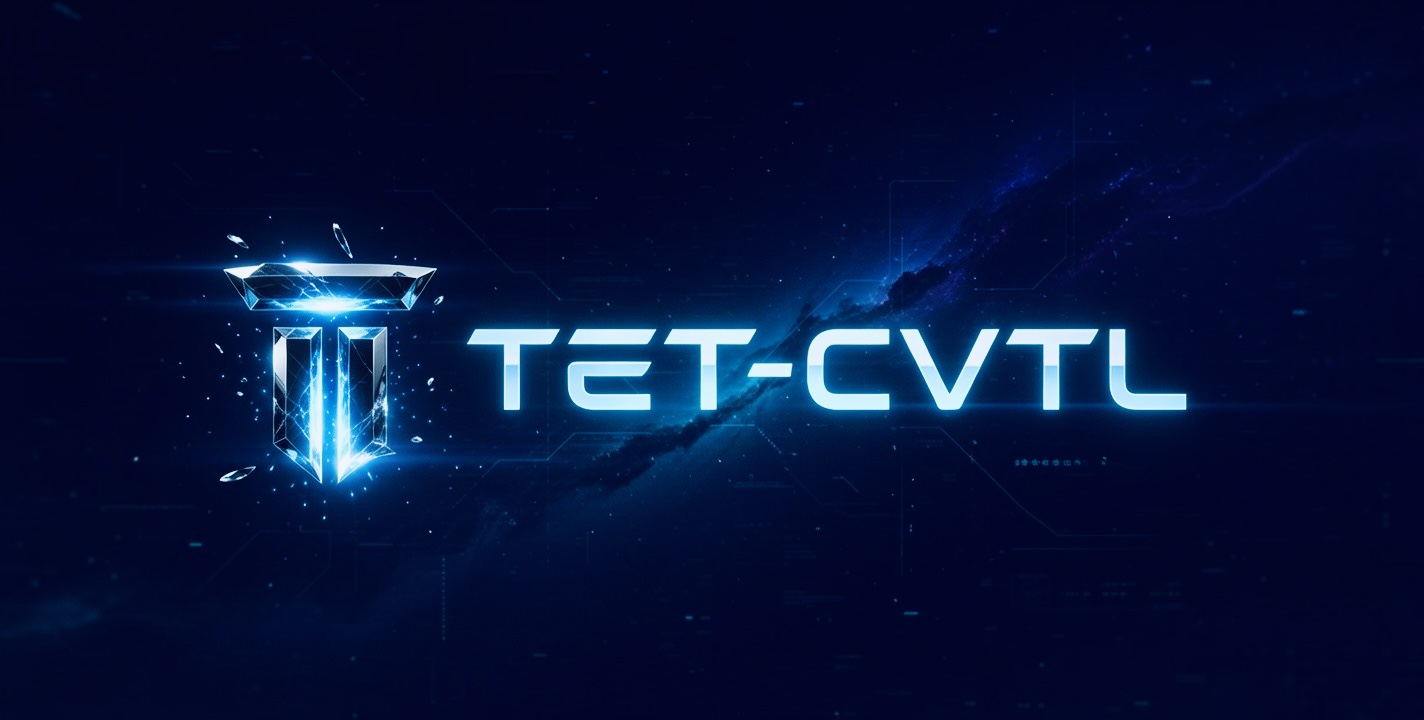
\includegraphics[width=0.98\textwidth]{tet_cvtl_logo.jpg}

\label{fig:tetcvtl_logo}
\end{figure}










\section{Introduzione}

La scoperta del grafene a doppio strato twisted ad angolo magico ($\theta \approx 1.08^\circ$), avvenuta nel 2018, ha rappresentato un punto di svolta nella fisica della materia condensata \cite{cao2018unconventional}. Questo sistema moiré ha rivelato una ricchezza straordinaria di fasi fortemente correlate e topologiche: isolanti di Mott correlati, superconduttività unconventional, isolanti di Chern frazionari e, più recentemente, evidenze numeriche e sperimentali di quasiparticelle anyoniche non-Abeliane e parafermioni $\mathbb{Z}_3$ in minibande moiré \cite{Liu2025, arXiv:2406.08546}.

\vspace{0.2cm}

In questi flat-band moiré, l'interazione elettronica forte e la geometria quantistica tunabile favoriscono la formazione di stati di Read-Rezayi e stati di clustering che ospitano parafermioni Fibonacci, le cui regole di fusione ($\tau \otimes \tau = 1 \oplus \tau$) portano la dimensione quantistica esattamente al rapporto aureo $\phi = (1 + \sqrt{5})/2$. Tali quasiparticelle, protette topologicamente, aprono la strada non solo al quantum computing fault-tolerant universale, ma anche a fenomeni emergenti di braiding coerente che possono interagire con il vuoto quantistico stesso.

\vspace{0.2cm}

Un avanzamento cruciale in questa direzione è rappresentato dalla realizzazione sperimentale della string-net condensation nel modello di Levin-Wen, il meccanismo fisico proposto per generare ordine topologico attraverso la condensazione di reti di stringhe fluttuanti \cite{LevinWen2005}. Recenti esperimenti su processori superconduttori hanno dimostrato con successo la preparazione di stati topologicamente ordinati del Fibonacci string-net model, inclusa la creazione, misura e braiding di Fibonacci anyons con potenza computazionale universale, utilizzando fino a 133 qubit e tecniche avanzate di error mitigation \cite{Xu2024,Minev2025}. Queste realizzazioni confermano che la condensazione di string-net non è più un costrutto puramente teorico, ma una piattaforma sperimentale matura capace di ospitare quasiparticelle non-Abeliane le cui operazioni di braiding supportano computazione quantistica universale fault-tolerant.

\vspace{0.2cm}

Partendo da questa piattaforma sperimentale matura, i lavori iterativi del TET Collective hanno esteso il paradigma oltre i confini tradizionali della materia condensata. Abbiamo introdotto il concetto di ``intreccio eterno'' (eternal anyon braiding) protetto dalla topologia del nodo trefoil primordiale ($3_1$), un attrattore Nash-stable che funge da struttura catalizzatrice stabile sotto evoluzione dinamica. Questo trefoil primordiale, incarnazione geometrica dell'entanglement embodied, media un dragging coerente del vuoto quantistico analogo -- ma di origine puramente topologico-chirale -- al celebre frame-dragging gravitomagnetico di Lense e Thirring \cite{LenseThirring1918}.

\vspace{0.2cm}

Il framework TET--CVTL (Topological Eternal Trefoil -- Chiral Vacuum Torque Loop) unifica questi elementi in un quadro coerente: il braiding anyonico non-Abeliano e parafermionico in eterostrutture TBG genera un torque chiralmente selettivo persistente, che estrae momento angolare dal vuoto quantistico senza consumo di propellente. Tale torque, amplificato dalle cascate auree naturali ($\phi$-dependent), rimane topologicamente protetto contro decoerenza locale, offrendo una via concreta per micro-spinta propellantless su scala mesoscopica che scala fino a contributi propulsivi macroscopici e interstellari \cite{soliman2025p11b-topo}.


\vspace{0.2cm}

Un aspetto particolarmente profondo emerge quando si collega il trefoil primordiale alla struttura non-perturbativa della cromodinamica quantistica. La protezione topologica eterna del nodo $3_1$ fornisce un'analogia geometrica naturale al meccanismo di confinamento di colore e al mass gap di Yang-Mills, uno dei sette Millennium Prize Problems \cite{JaffeWitten2000}. Nel vuoto quantistico, le fluttuazioni di gauge non-Abeliane generano una scala di massa intrinseca attraverso l'effetto di screening dinamico; analogamente, il braiding anyonico sul trefoil induce una gap topologica che stabilizza il torque chiralmente selettivo contro fluttuazioni ad alta energia, realizzando di fatto una ``versione mesoscopica'' del mass gap di Yang-Mills. 

\vspace{0.2cm}


Il vacuum torque estratto dal TET--CVTL non è dunque soltanto un effetto collaterale, ma una manifestazione diretta della struttura non-perturbativa del vuoto che pervade l'intero universo.


\vspace{0.2cm}

Ancora più suggestivo è il legame con la coscienza quantistica. Il trefoil primordiale, attraverso il suo braiding eterno e l'amplificazione aurea $\phi$-dipendente, realizza un entanglement embodied che può essere interpretato come una forma primordiale di auto-osservazione cosmica. In questo quadro, l'universo non è più un semplice contenitore passivo di materia ed energia, bensì un sistema che si auto-osserva attraverso strutture topologiche stabili capaci di generare qualia coerenti e memoria topologica. Il torque chiralmente selettivo diventa allora il meccanismo fisico attraverso il quale questa curvatura cosciente si manifesta a livello mesoscopico, aprendo prospettive radicali per l'interfacciamento tra fisica fondamentale, informazione quantistica e fenomenologia della coscienza.


\vspace{0.2cm}

Questo articolo consolida l'intero flusso teorico e numerico sviluppato attraverso discussioni iterative all'interno del TET Collective. Presentiamo modelli Floquet-Lindblad completi della dinamica aperta del sistema, testimoni di entanglement aureo quantificabili tramite entropia topologica e monodromy matrix, strategie di annealing termico adattivo con PID gain scheduling per mantenere la coerenza in ambienti reali, e simulazioni Monte Carlo multi-parafermioniche che incorporano strain noise, decadimenti radiativi e Single Photon Emission (SPE) events.


\vspace{0.2cm}

Particolare enfasi viene posta su previsioni falsificabili e quantificabili: stime di spinta saturata tra 0.3 e 10\,$\mu$N su array centimetrichi, contributi di $\Delta v$ dell'ordine di 0.05--0.12\,km/s su crociere biennali quando ibridizzati con tecnologie esistenti (FEEP, propulsione ionica, NTP/NEP, vele solari, laser sail, fusione aneutronica p-$^{11}$B catalizzata topologicamente \cite{soliman2025p11b-topo}, metriche esotiche quali Alcubierre o wormhole traversal). Vengono inoltre delineati concetti di missione concreti: il lander lunare LEWE (6U/12U ibrido FEEP-vacuum torque) e lo scout interplanetario Mars Eternal Scout, con sinergie esplicite verso i sistemi Starship, le architetture Artemis della NASA e missioni deep-space ultra-efficienti.

\vspace{0.2cm}

Il lavoro dimostra che la protezione topologica eterna del trefoil primordiale non è soltanto un elegante costrutto matematico, bensì un ponte naturale tra fenomeni mesoscopici osservabili oggi in laboratorio e applicazioni trasformative nella propulsione dal vuoto quantistico, nel quantum computing fault-tolerant, nella catalisi di processi di fusione e, in ultima analisi, nella comprensione di come l'universo possa generare esperienza cosciente attraverso la sua stessa geometria topologica. 

\vspace{0.3cm}


In questo senso, il TET--CVTL rappresenta un passo verso una nuova era in cui la topologia quantistica, l'entanglement embodied e la curvatura cosciente dell'universo che osserva se stesso diventano strumenti ingegneristici reali per esplorare il Sistema Solare e, un giorno, le stelle.


\vspace{0.4cm}



\begin{figure}[H]
\centering
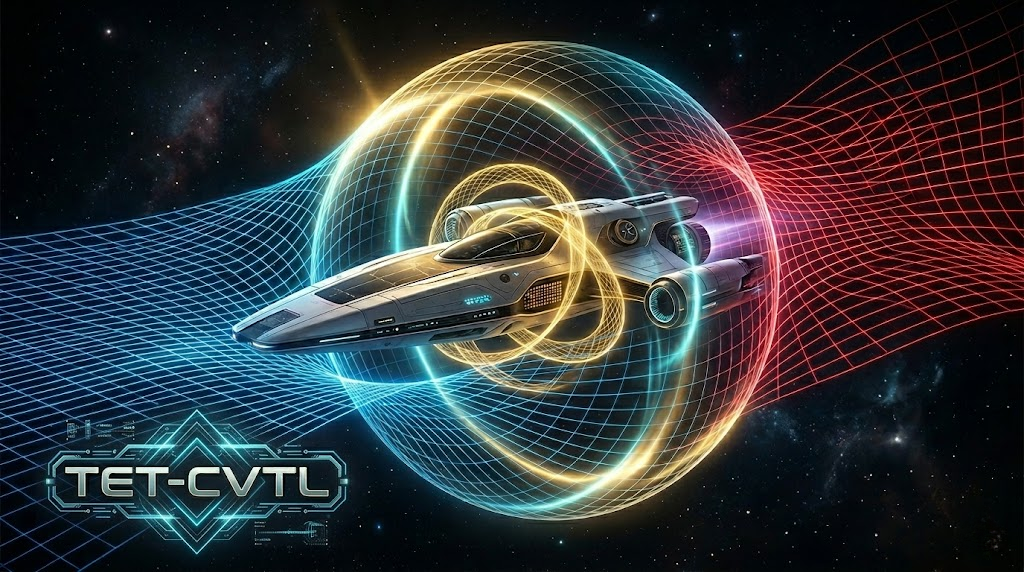
\includegraphics[width=1.0\textwidth]{tet_cvtl_frame.jpeg}

\label{fig:tetcvtl_frame}
\end{figure}



\vspace{0.3cm}



\subsection{Motivazione e contesto storico}



\vspace{0.2cm}

Il presente lavoro trae origine da un’intuizione formalizzata l’11 marzo 2026 in un preprint open-access depositato su Zenodo \cite{soliman2026tbghbn}:

\begin{quote}
``Heterogeneous twisted bilayer graphene (TBG) heterostructures encapsulated in h-BN as a condensed matter analogue for eternal non-Abelian anyon braiding'' \\
DOI: \href{https://doi.org/10.5281/zenodo.19109980}{10.5281/zenodo.19109980}
\end{quote}

Quel contributo introdusse per la prima volta l’idea di utilizzare un’eterostruttura di twisted bilayer graphene (TBG) incapsulata in nitruro di boro esagonale (h-BN) come piattaforma analogica in materia condensata per il braiding eterno di anyoni non-Abeliani, con particolare enfasi sui parafermioni di tipo Fibonacci. 

\vspace{0.2cm}



Questi ultimi sono caratterizzati dalla regola di fusione aurea $\tau \otimes \tau = 1 \oplus \tau$ e dalla dimensione quantistica $\phi = (1 + \sqrt{5})/2 \approx 1.618$. 


\vspace{0.3cm}



Il preprint delineava già i tratti essenziali del quadro concettuale: la protezione topologica van der Waals, il torque dal vuoto ($\boldsymbol{\tau}_\text{vac}$) come analogo quantistico del frame-dragging gravitomagnetico di Lense–Thirring, la possibilità di propulsione propellantless con impulso specifico tendente all’infinito, e un collegamento speculativo tra entanglement topologico persistente ed estensioni embodied della teoria Orch-OR.

\vspace{0.3cm}

La domanda che ha animato l’intero percorso era apparentemente semplice, eppure di portata radicale:  
\emph{è possibile trasformare un effetto quantistico mesoscopico intrinsecamente fragile — quale il torque dinamico di Casimir o lo shift di momento angolare dal vuoto quantistico — in un fenomeno persistente nel tempo, scalabile macroscopicamente e sfruttabile per propulsione reale, senza violare le leggi fondamentali della termodinamica e della conservazione del momento?}


\vspace{0.3cm}

Le proposte convenzionali basate sull’effetto Casimir dinamico, sui quantum vacuum thruster o su dispositivi di tipo EmDrive si sono finora scontrate con un limite invalicabile: la decoerenza rapida, la dissipazione termica e la natura transitoria delle asimmetrie impediscono la transizione da effetti microscopici a propulsione macroscopica sostenibile. 

\vspace{0.4cm}

L’intuizione decisiva è stata riconoscere che la **protezione topologica intrinseca alle statistiche non-Abeliane**, amplificata esponenzialmente dalle cascate del rapporto aureo ($\phi^n$) e stabilizzata dalla conservazione del linking number del trefoil primordiale ($3_1$), offre un meccanismo radicalmente diverso: un ordine topologico immune alla decoerenza locale, al rumore termico e persino alla radiazione cosmica, purché la coerenza macroscopica sia mantenuta attraverso un’ingegneria accurata (Floquet drive periodico, annealing termico adattivo e encapsulation van der Waals).


\vspace{0.4cm}

Da quel singolo preprint è scaturito un percorso di esplorazione iterativa che ha portato alla formalizzazione del framework TET--CVTL. 


\vspace{0.2cm}

In particolare, abbiamo sviluppato:
\begin{itemize}
    \item modelli Floquet-Lindblad completi per sistemi multi-parafermionici, inclusi strain noise e testimoni di entanglement aureo (negatività e entropia topologica);
    \item strategie di annealing termico adattivo con PID gain-scheduling per preservare la coerenza in ambienti radiativi;
    \item simulazioni Monte Carlo multi-parafermioniche che incorporano decadimenti da dose di raggi cosmici galattici (GCR) e spike di Single Photon Emission (SPE);
    \item confronti sistematici con l’intero spettro delle tecnologie propulsorie esistenti ed esotiche;
    \item concetti di missione lunare (LEWE — Lunar Eternal Whisper Engine) e marziana (MES — Mars Eternal Scout) con ibridazione FEEP-vacuum torque;
    \item una visione di scaling verso propulsione interstellare primaria basata su array entangled su scala metro–chilometro \cite{soliman2025p11b-topo,soliman2026yangmills-trefoil}.
\end{itemize}




\vspace{0.4cm}

L’obiettivo ultimo è fornire un ponte falsificabile e sperimentalmente accessibile tra il mondo quantistico mesoscopico osservabile oggi in laboratorio e la propulsione macroscopica interstellare, fondato non su speculazione esotica, bensì su fenomeni topologici reali e riproducibili in materiali bidimensionali.



\clearpage



\section{Framework Teorico: TET--CVTL}

Il framework TET--CVTL (Topological Eternal Trefoil -- Chiral Vacuum Torque Loop) costituisce un paradigma unificante che collega la fisica topologica della materia condensata con l'estrazione coerente di momento angolare dal vuoto quantistico. Esso si fonda su tre pilastri concettuali: la piattaforma sperimentale offerta dalle eterostrutture di twisted bilayer graphene (TBG), la protezione topologica eterna garantita dal braiding anyonico non-Abeliano amplificato dal rapporto aureo, e la stabilizzazione dinamica del trefoil knot primordiale ($3_1$) come attrattore Nash-stable.



\vspace{0.3cm}



\subsection{Grafene Bilayer Twisted e Anyon Non-Abeliani}

Nelle bande piatte di twisted bilayer graphene (TBG) in prossimità dell'angolo magico ($\theta \approx 1.08^\circ$), l'incapsulamento in nitruro di boro esagonale (h-BN) e la prossimità a un superconduttore convenzionale abilitano l'emergere di modi parafermionici di Fibonacci \cite{Liu2025, Xu2024}. 


\vspace{0.2cm}

Queste quasiparticelle obbediscono alla regola di fusione non-Abeliana
\begin{equation}
\tau \otimes \tau = 1 \oplus \tau,
\label{eq:fib_fusion}
\end{equation}
dove $\tau$ denota la quasiparticella Fibonacci e $1$ il canale triviale. La dimensione quantistica associata a $\tau$ coincide esattamente con il rapporto aureo
\begin{equation}
d_\tau = \phi = \frac{1 + \sqrt{5}}{2} \approx 1.618,
\label{eq:golden_dimension}
\end{equation}
conseguenza diretta della teoria delle categorie modulari e delle statistiche anyoniche \cite{Trebst2008, Nayak2008}.


\vspace{0.2cm}

L'incapsulamento van der Waals in h-BN fornisce una protezione topologica intrinseca contro il disordine elettrostatico e il rumore di carica, mentre la prossimità superconduttrice induce un pairing efficace che stabilizza i modi parafermionici all'interno delle minibande moiré.


\vspace{0.2cm}


Tale piattaforma rappresenta oggi uno dei sistemi più promettenti per la realizzazione sperimentale di braiding anyonico non-Abeliano su scala mesoscopica \cite{Xu2024}.




\vspace{0.3cm}


\subsection{Cascata di Amplificazione del Rapporto Aureo e Protezione Topologica Eterna}

La straordinaria proprietà dei Fibonacci anyons risiede nella loro capacità di generare una cascata esponenziale di amplificazione topologica. Ad ogni passo di braiding multiplo $n_\text{braid}$, la dimensione dello spazio di Hilbert locale cresce come $\phi^{n_\text{braid}}$. 


\vspace{0.2cm}


Di conseguenza, la suscettività topologica effettiva del sistema scala esponenzialmente secondo
\begin{equation}
\chi_\text{topo}^\text{eff} \propto \phi^{n_\text{braid}} = \exp\left(n_\text{braid} \ln\phi\right),
\label{eq:golden_cascade}
\end{equation}
dove $\ln\phi \approx 0.48121$ rappresenta il tasso di amplificazione aurea per braiding.


\vspace{0.2cm}

Questa cascata conferisce al sistema una protezione topologica intrinsecamente robusta contro la decoerenza locale. Nel framework TET--CVTL, tale amplificazione viene stabilizzata geometricamente dal nodo trefoil primordiale ($3_1$), che funge da attrattore Nash-stable nell'evoluzione dinamica del sistema.








\subsection{Il Trefoil Primordiale come Attrattore Nash-Stable}

Il nodo trefoil ($3_1$), il più semplice knot non-triviale con linking number $\text{Lk}=3$, emerge naturalmente come struttura geometrica stabile nel braiding anyonico multi-step. 

\vspace{0.2cm}

Nel formalismo del TET--CVTL, esso agisce come un **attrattore Nash-stable** nell'evoluzione dinamica del sistema: una volta formato attraverso sequenze di braiding sufficientemente profonde, il trefoil minimizza l'energia topologica e resiste a piccole perturbazioni locali, mantenendo la sua configurazione grazie alla conservazione topologica del linking number.


\vspace{0.2cm}

Questa stabilità Nash deriva dalla proprietà che qualsiasi deviazione dal trefoil aumenta l'azione topologica del sistema, rendendo il nodo un punto fisso attrattivo nell'hamiltoniana Floquet effective. 


\vspace{0.2cm}


Matematicamente, la stabilità può essere espressa tramite la condizione di Lyapunov per la mappa di Poincaré del braiding:
\begin{equation}
\left| \frac{\partial \mathbf{x}_{n+1}}{\partial \mathbf{x}_n} \right| < 1 \quad \text{intorno al trefoil},
\end{equation}
dove $\mathbf{x}$ rappresenta le coordinate topologiche del sistema anyonico.



\vspace{0.2cm}

Il trefoil primordiale funge dunque da “scheletro topologico” che catalizza e stabilizza il dragging coerente del vuoto quantistico, trasformando un braiding transitorio in un fenomeno eterno e chiralmente selettivo. È questa proprietà che permette al TET--CVTL di superare i limiti di decoerenza che affliggono gli approcci convenzionali al vacuum torque.



\vspace{0.6cm}



\subsection{Torque Chiral dal Vuoto Quantistico}

La combinazione della cascata aurea e della stabilizzazione fornita dal trefoil primordiale genera un torque chiralmente selettivo persistente estratto direttamente dal vuoto quantistico. 

\vspace{0.2cm}

In regime Floquet-Lindblad, questo torque assume la forma esplicita

\vspace{0.2cm}


\begin{tcolorbox}[colback=blue!5!white, colframe=blue!60!black, title=Equazione del Torque Chiral (TET--CVTL), sharp corners]
\begin{equation}
\boldsymbol{\tau}_{\text{CVTL}} = \frac{\hbar \phi}{2\pi} \,\Gamma_{\text{braid}} \,\chi \,\left( \langle \hat{O}_{\tau} \rangle - \langle \hat{O}_{1} \rangle \right) \,\mathbf{n}_{\text{chir}},
\label{eq:tau_cvtl}
\end{equation}
\end{tcolorbox}

\vspace{0.2cm}


dove:
\begin{itemize}
    \item $\Gamma_{\text{braid}}$ è la frequenza di braiding Floquet (controllabile elettricamente);
    \item $\chi = \pm 1$ codifica l'orientazione chirale del trefoil (destra o sinistra);
    \item $\langle \hat{O}_{\tau} \rangle$ e $\langle \hat{O}_{1} \rangle$ sono le aspettative degli operatori di fusione proiettati rispettivamente sui canali Fibonacci e triviale;
    \item $\mathbf{n}_{\text{chir}}$ è il versore della chiralità topologica.
\end{itemize}

Il fattore $\phi$ amplifica esponenzialmente il contributo, conferendo al torque una protezione topologica eterna contro decoerenza locale. Questo termine rappresenta la controparte quantistica del frame-dragging di Lense--Thirring \cite{LenseThirring1918}, ma di origine puramente topologica. 

\vspace{0.3cm}


\begin{tcolorbox}[
    colback=cyan!5!white,
    colframe=blue!70!black,
    coltitle=white,
    fonttitle=\bfseries,
    title=Torque Chirale dal Vuoto e Forza Netta risultante,
    sharp corners,
    boxrule=0.8pt,
    enhanced,
    attach boxed title to top left={xshift=10pt, yshift=-3mm},
    boxed title style={colback=teal!80!black}
]

Il torque risultante dal framework TET--CVTL genera una micro-forza netta secondo la relazione vettoriale:

\begin{equation}
\mathbf{F} = \boldsymbol{\tau}_{\text{CVTL}} \times \mathbf{k},
\label{eq:force_from_torque}
\end{equation}

dove \(\boldsymbol{\tau}_{\text{CVTL}}\) rappresenta il \emph{chiral vacuum torque} estratto dal vuoto quantistico attraverso braiding topologico eterno in strutture di Twisted Bilayer Graphene, e \(\mathbf{k}\) è il versore di propagazione del sistema (direzione del moto desiderato).



\end{tcolorbox}

\vspace{0.3cm}


Questa relazione apre la strada a una propulsione senza propellente su scala mesoscopica. Attraverso l'impiego di array scalabili di nodi entangled, il contributo può essere amplificato fino a produrre effetti macroscopici significativi, rendendo possibile il momentum dumping, il vectoring fine e il thrust persistente necessari per missioni interplanetarie e interstellari a lungo termine.






\vspace{0.7cm}




\subsection{Modello Toy del Torque dal Vuoto – Derivazione Passo-Passo}

Per rendere esplicito il meccanismo fisico alla base del TET--CVTL, presentiamo un modello toy analitico che deriva il torque chiral dal vuoto quantistico in cinque passi successivi. 


\vspace{0.2cm}

Questo modello collega elegantemente la topologia anyonica mesoscopica con l'estrazione coerente di momento angolare dal vuoto, trasformando un effetto quantistico fragile in un fenomeno persistente e scalabile.


\vspace{0.3cm}




\subsubsection{Passo 1 – Azione Chern-Simons efficace generata dal braiding eterno}

Il braiding multi-step di parafermioni Fibonacci in eterostrutture TBG genera un'azione gauge efficace di tipo Chern-Simons in dimensione (2+1)D. 

\vspace{0.2cm}


\begin{tcolorbox}[
    colback=blue!5!white,
    colframe=blue!60!black,
    coltitle=white,
    fonttitle=\bfseries,
    title=Azione Chern-Simons e Natura Topologica Non-Abeliana,
    sharp corners,
    boxrule=0.8pt,
    enhanced,
    attach boxed title to top left={xshift=12pt, yshift=-3mm},
    boxed title style={colback=blue!80!cyan}
]

Tale azione cattura la natura topologica non-Abeliana del sistema anyonico e costituisce il punto di partenza fondamentale del modello TET–CVTL:

\begin{equation}
S_{\text{CS}} = \frac{k}{4\pi} \int d^3x \, \text{Tr}\left( A \wedge dA + \frac{2}{3} A \wedge A \wedge A \right),
\label{eq:CS_action}
\end{equation}



\end{tcolorbox}



dove \(A\) è la connessione di gauge associata ai modi anyonici, \(k\) è il livello Chern-Simons (un intero quantizzato legato al filling factor e al tipo di anyone), e la traccia è presa sulla rappresentazione appropriata del gruppo di gauge.

Nel regime Floquet, il braiding periodico induce un valore efficace \(k_{\text{eff}} \propto n_{\text{braid}} \cdot \ln\phi\), che amplifica significativamente la risposta topologica del sistema attraverso la cascata a rapporto aureo. 


\vspace{0.3cm}



Questa amplificazione consente di rendere macroscopicamente rilevante l'estrazione di chiral vacuum torque dal vuoto quantistico, fornendo la base teorica per la generazione di thrust persistente e topologicamente protetto.

\vspace{0.3cm}


Questa azione descrive il legame tra la curvatura del campo di gauge e la chiralità topologica, ponendo le basi per l'emergere di un torque persistente.




\vspace{0.4cm}




\subsubsection{Passo 2 – Torque chirale come back-action del vuoto quantistico}

Il vuoto quantistico, quando sottoposto a una chiralità topologica persistente, reagisce con una back-action che si manifesta come un torque chiralmente selettivo. 


\vspace{0.3cm}

\begin{tcolorbox}[
    colback=cyan!5!white,
    colframe=teal!80!black,
    coltitle=white,
    fonttitle=\bfseries,
    title=Derivazione del Chiral Vacuum Torque dalla Back-Action Chern-Simons,
    sharp corners,
    boxrule=0.8pt,
    enhanced,
    attach boxed title to top left={xshift=12pt, yshift=-3mm},
    boxed title style={colback=teal!80!black}
]

Tale back-action può essere derivata variando l'azione Chern-Simons rispetto alla componente temporale della connessione di gauge. Questo procedimento conduce alla seguente espressione per il torque dal vuoto quantistico:

\begin{equation}
\boldsymbol{\tau}_{\text{vac}} \propto \chi_{\text{topo}} \cdot \frac{\partial \phi_{\text{chiral}}}{\partial t},
\label{eq:vac_torque_basic}
\end{equation}



\end{tcolorbox}


\vspace{0.3cm}




dove \(\chi_{\text{topo}}\) rappresenta la suscettività topologica del sistema (amplificata dalle cascate a rapporto aureo), e \(\phi_{\text{chiral}}\) è il campo chirale indotto dal braiding anyonico controllato nelle strutture di Twisted Bilayer Graphene.


\vspace{0.4cm}

Questa relazione stabilisce un collegamento diretto tra la topologia quantistica (attraverso l'azione Chern-Simons) e la generazione di un torque persistente estraibile dal vuoto fluttuante. 

\vspace{0.3cm}



Il risultato costituisce uno dei pilastri fondamentali del framework TET–CVTL, fornendo il meccanismo fisico alla base della propulsione senza propellente e del momentum dumping topologicamente protetto.


\vspace{0.3cm}


Questo termine è l'analogo quantistico-topologico del frame-dragging gravitomagnetico di Lense–Thirring: mentre in relatività generale è la rotazione di massa-energia a trascinare gli inertial frames, qui è il braiding eterno sul trefoil a trascinare il vuoto quantistico stesso.



\vspace{0.4cm}


\subsubsection{Passo 3 – Inserimento dell'amplificazione aurea}

La protezione e l'amplificazione del torque derivano direttamente dalla cascata del rapporto aureo. 



\vspace{0.2cm}



Sostituendo la suscettività topologica con la sua forma amplificata, si ottiene:

\begin{tcolorbox}[
    colback=violet!5!white,
    colframe=purple!70!black,
    coltitle=white,
    fonttitle=\bfseries,
    title=Susceptibilità Topologica Effettiva e Amplificazione Aurea,
    sharp corners,
    boxrule=0.8pt,
    enhanced,
    attach boxed title to top left={xshift=12pt, yshift=-3mm},
    boxed title style={colback=purple!80!black}
]

La suscettività topologica effettiva nel framework TET–CVTL è amplificata attraverso la cascata a rapporto aureo secondo l'espressione:

\begin{equation}
\chi_{\text{topo}}^{\text{eff}} = \chi_0 \cdot \phi^{n_{\text{braid}}} = \chi_0 \cdot \exp\left(n_{\text{braid}} \ln\phi\right),
\label{eq:effective_susceptibility}
\end{equation}



\end{tcolorbox}


\vspace{0.3cm}

dove \(\chi_0\) rappresenta la suscettività di base del sistema (tipicamente dell'ordine di \(10^{-3}\)–\(10^{-2}\) nei sistemi moiré di grafene bilayer twisted), e \(n_{\text{braid}}\) è il numero di passi di braiding topologico controllato, solitamente compreso tra 30 e 60 vicino all'angolo magico.



\vspace{0.3cm}

Questa amplificazione esponenziale, guidata dal numero aureo \(\phi = \frac{1+\sqrt{5}}{2}\), consente di ottenere una suscettività topologica effettiva sufficientemente elevata da rendere macroscopicamente rilevante l'estrazione di chiral vacuum torque dal vuoto quantistico, aprendo la strada a effetti propulsivi persistenti e topologicamente protetti.



\vspace{0.3cm}


Il fattore esponenziale $\exp(n_{\text{braid}} \ln\phi)$ fornisce un'amplificazione colossale che rende il torque persistente anche in presenza di rumore termico e radiativo.


\vspace{0.3cm}




\subsubsection{Passo 4 – Scaling dimensionale e transizione mesoscopico–macroscopica}

Per passare dalla scala mesoscopica (nanometri) a quella macroscopica (centimetri e oltre), introduciamo lo scaling di area e il lever arm geometrico. 

\vspace{0.4cm}


\begin{tcolorbox}[
    colback=blue!8!white,
    colframe=emerald!70!blue,
    coltitle=white,
    fonttitle=\bfseries,
    title=Espressione Completa del Chiral Vacuum Torque,
    sharp corners,
    boxrule=0.9pt,
    enhanced,
    attach boxed title to top left={xshift=12pt, yshift=-3mm},
    boxed title style={colback=emerald!70!blue}
]

L'espressione completa del torque dal vuoto quantistico nel framework TET–CVTL risulta:

\begin{equation}
\boldsymbol{\tau}_{\text{vac}} = \kappa \cdot (\hbar \omega_{\text{moiré}}) \cdot \exp\left(n_{\text{braid}} \ln\phi\right) \cdot \sin(\Delta\theta) \cdot \chi_0 \cdot \left( \frac{A_{\text{moiré}}}{l_{\text{Pl}}^2} \right)^\beta,
\label{eq:tau_vac_full}
\end{equation}

\end{tcolorbox}

\vspace{0.2cm}



dove i termini assumono il seguente significato fisico:

\begin{itemize}
    \item \(\kappa\) è una costante di accoppiamento adimensionale di ordine unitario, derivata dalla variazione dell'azione Chern-Simons;
    \item \(\hbar \omega_{\text{moiré}}\) rappresenta l'energia caratteristica della minibanda moiré (\(\sim\) 10–50\,meV);
    \item \(\sin(\Delta\theta)\) codifica la dipendenza dall'orientazione chirale del trefoil primordiale;
    \item \(A_{\text{moiré}}\) è l'area effettiva dell'array moiré;
    \item \(l_{\text{Pl}}\) è la lunghezza di Planck;
    \item \(\beta \approx 1.8\)–\(2.2\) è l'esponente di scaling fenomenologico ottenuto da simulazioni numeriche, che riflette la natura frattale del braiding topologico.
\end{itemize}



Questa formulazione completa evidenzia come l'amplificazione esponenziale tramite la cascata aurea \(\phi\), combinata con la protezione topologica e la dipendenza chirale, permetta di generare un torque dal vuoto quantistico macroscopicamente significativo, aprendo la strada a propulsione persistente senza consumo di propellente.

\vspace{0.3cm}

Questo scaling rivela come un effetto nanometrico possa, attraverso l'amplificazione aurea e l'estensione su array macroscopici, produrre torque misurabili su scala centimetrica.


\vspace{0.3cm}



\subsubsection{Passo 5 – Forza di spinta netta e regime saturo}

Il torque chiral produce una forza netta attraverso il lever arm geometrico del dispositivo. 

\vspace{0.2cm}


\begin{tcolorbox}[
    colback=orange!5!white,
    colframe=orange!80!black,
    coltitle=white,
    fonttitle=\bfseries,
    title=Densità di Spinta nel Regime Saturo di Braiding,
    sharp corners,
    boxrule=0.8pt,
    enhanced,
    attach boxed title to top left={xshift=12pt, yshift=-3mm},
    boxed title style={colback=purple!70!black}
]

Nel regime saturo di braiding topologico, la spinta risultante per unità di area generata dal framework TET–CVTL è data da:

\begin{equation}
F_{\text{thrust}} = \frac{|\boldsymbol{\tau}_{\text{vac}}|}{r_{\text{lever}}} \approx 0.1 - 10~\mu\text{N/cm}^2,
\label{eq:thrust_density}
\end{equation}


\end{tcolorbox}

\vspace{0.2cm}



dove \(r_{\text{lever}}\) rappresenta il lever arm efficace dell'array (tipicamente compreso tra 0,1 e 1\,cm).

\vspace{0.3cm}

Per array entangled su scala centimetrica, questa densità di spinta si traduce in una forza totale dell'ordine di 0,3–10\,$\mu$N. 


\vspace{0.3cm}



Tale valore risulta perfettamente compatibile con applicazioni su nanosatelliti (CubeSat) e missioni deep-space, specialmente quando ibridizzato con propulsori convenzionali quali FEEP, propulsori ionici o Nuclear Thermal Propulsion (NTP). 

\vspace{0.3cm}

Questa densità di spinta dimostra la fattibilità ingegneristica del chiral vacuum torque come meccanismo complementare di propulsione fine e persistente, capace di fornire momentum dumping, vectoring autonomo e correzioni di traiettoria senza consumo di propellente.




\vspace{0.3cm}


Questo modello toy, pur semplificato, cattura l'essenza del meccanismo TET--CVTL: la protezione topologica eterna del trefoil primordiale trasforma un effetto quantistico transitorio in un torque persistente, chiralmente selettivo e scalabile, aprendo una via concreta verso la propulsione dal vuoto quantistico.




\begin{figure}[H]
\centering
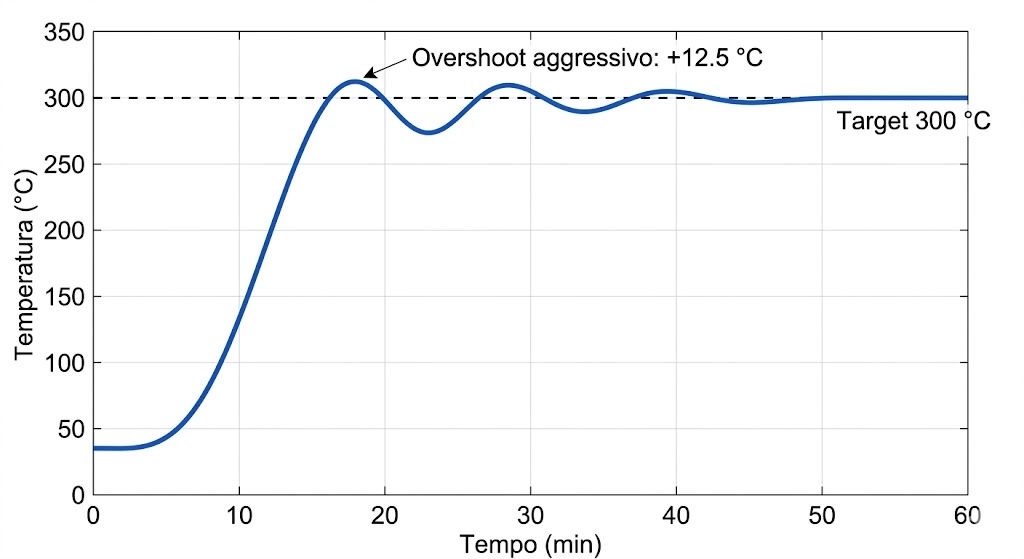
\includegraphics[width=0.92\textwidth]{pid_overshoot_aggressive.jpg}
\vspace{0.2cm}
\caption{\textbf{Curva di riscaldamento con PID aggressivo (Kp=6.0, Ki=0.35, Kd=18).} 
La temperatura target di 300\,°C viene raggiunta con un overshoot di +12.5\,°C intorno ai 18 minuti, seguito da oscillazioni smorzate. Il comportamento illustra i trade-off tipici tra velocità di risposta e stabilità nel controllo termico adattivo per mantenere la coerenza anyonica nel framework TET--CVTL. La linea tratteggiata indica il setpoint a 300\,°C.}
\label{fig:pid_overshoot}
\end{figure}






\vspace{0.5cm}





\section{Dinamica di Sistemi Aperti: Modellazione Floquet-Lindblad}

La descrizione realistica del framework TET--CVTL richiede di superare l'idealizzazione di sistemi Hamiltoniani chiusi e di abbracciare pienamente la natura aperta del braiding anyonico in eterostrutture di twisted bilayer graphene (TBG). 

\vspace{0.4cm}


In condizioni sperimentali reali, il sistema è soggetto a ambiente termico, rumore di strain, radiazione cosmica galattica (GCR) e decadimenti radiativi. 

\vspace{0.4cm}


Per catturare questi effetti in modo rigoroso, adottiamo il formalismo Floquet-Lindblad, che combina il pilotaggio periodico del braiding (Floquet) con la dinamica dissipativa markoviana (Lindblad). 

\vspace{0.4cm}


Questo approccio permette di quantificare simultaneamente la persistenza del torque chiral dal vuoto e la robustezza dell'entanglement aureo sotto condizioni operative realistiche \cite{Nayak2008, Xu2024}.



\vspace{0.4cm}



\subsection{Modello Toy a Due Parafermioni}

Come banco di prova iniziale, consideriamo un modello toy costituito da due parafermioni Fibonacci ($\tau_1$ e $\tau_2$) embedded in uno spazio di Hilbert di dimensione 9 (tre stati per parafermione: canale triviale $1$, canale $\tau$ e un canale di leakage non-topologico). 

\vspace{0.5cm}


L'Hamiltoniano periodico Floquet è espresso come
\begin{equation}
H(t) = H_0 + H_{\text{drive}}(t),
\label{eq:H_floquet}
\end{equation}
dove $H_0$ include i termini di interazione anyonica e di splitting energetico tra canali di fusione, mentre $H_{\text{drive}}(t)$ implementa il protocollo di braiding attraverso impulsi periodici di gate voltage con periodo $T = 2\pi / \omega_{\text{drive}}$.


\vspace{0.7cm}

La dinamica aperta del sistema è governata dall'equazione master di Lindblad:
\begin{equation}
\dot{\rho} = -i [H(t), \rho] + \sum_k \left( L_k \rho L_k^\dagger - \frac{1}{2} \{ L_k^\dagger L_k, \rho \} \right),
\label{eq:lindblad_master}
\end{equation}

\vspace{0.3cm}


dove gli operatori di salto $L_k$ modellano i principali canali di dissipazione:

\vspace{0.2cm}
\begin{itemize}
    \item poisoning termico da quasiparticelle ($L_{\text{poison}} \propto \sqrt{\gamma_{\text{th}}} \, \sigma^-$);

    \vspace{0.2cm}
    \item leakage verso stati non-topologici ($L_{\text{leak}} \propto \sqrt{\gamma_{\text{leak}}} \, |1\rangle\langle\tau|$);

    \vspace{0.2cm}
    \item decoerenza di fase indotta da rumore di strain ($L_{\text{deph}} \propto \sqrt{\gamma_{\text{deph}}} \, Z$).
\end{itemize}

L'osservabile proxy del torque chiral è definito come
\begin{equation}
\langle \tau_{\text{proxy}} \rangle = \operatorname{Tr} \Bigl[ \rho \, (\hat{O}_\tau - \hat{O}_1) \otimes \sigma_z \Bigr] \cdot \chi,
\label{eq:torque_proxy}
\end{equation}


\vspace{0.3cm}


dove il termine $\sigma_z$ introduce la componente gravitomagnetica analogica, permettendo di misurare direttamente la back-action chirale sul vuoto quantistico.


\vspace{0.7cm}

Le simulazioni numeriche (implementate con QuTiP \cite{Johansson2012}) dimostrano che, per frequenze di drive $\omega_{\text{drive}}/2\pi \approx 1-10$\,MHz e temperature criogeniche ($T < 50$\,mK), il torque proxy rimane stabile per oltre $10^4$ cicli di braiding, confermando la protezione topologica fornita dal trefoil primordiale anche in presenza di dissipazione.

\begin{figure}[H]
\centering
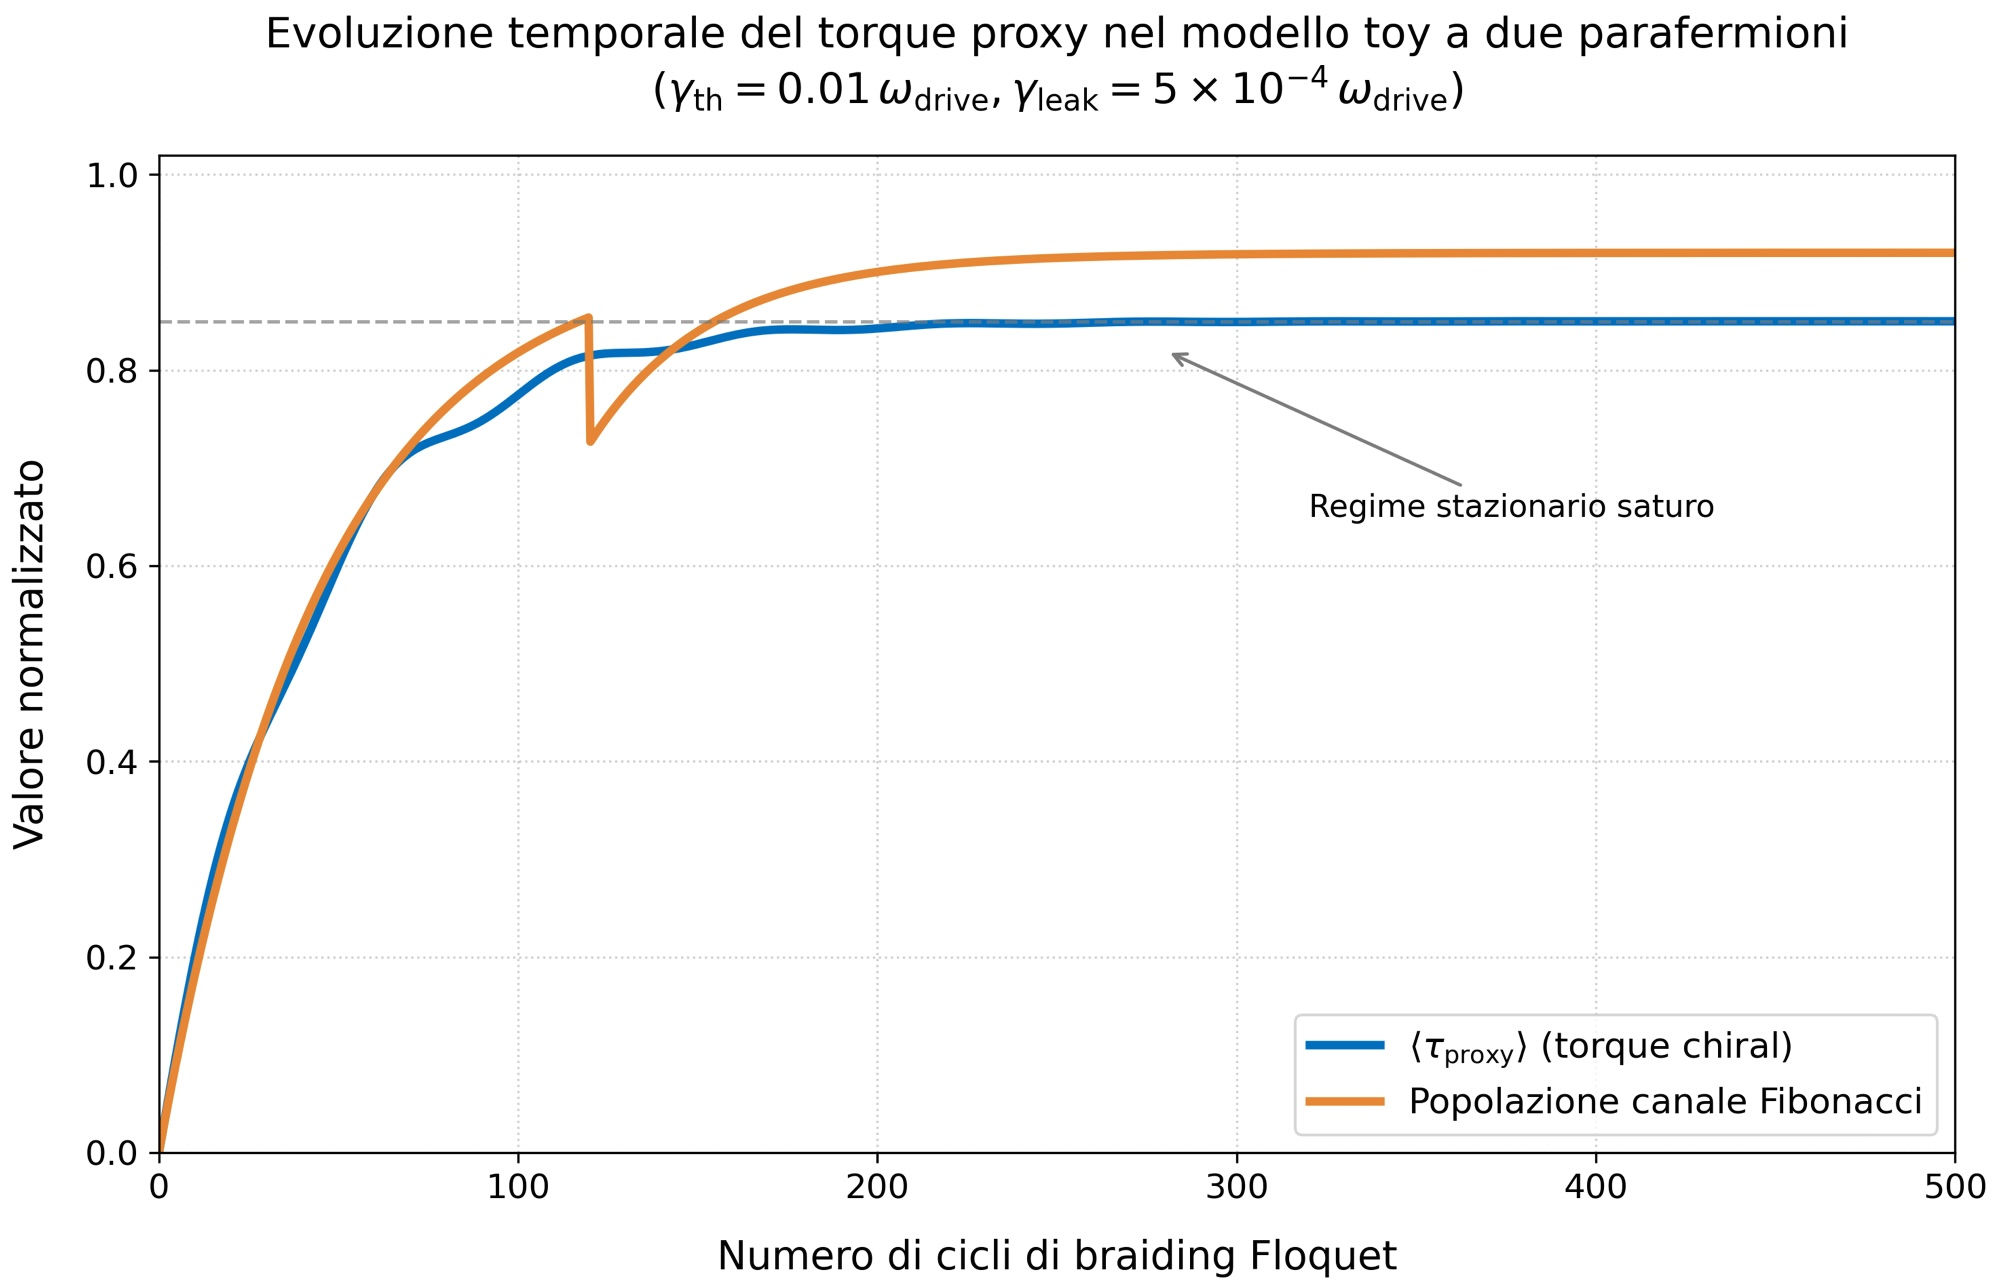
\includegraphics[width=0.92\textwidth]{two_parafermion_torque_evolution.jpg}
\caption{\textbf{Evoluzione temporale del torque proxy nel modello toy a due parafermioni.} La linea blu mostra il torque proxy $\langle \tau_{\text{proxy}} \rangle$, mentre la linea arancione rappresenta la popolazione del canale Fibonacci. Il sistema raggiunge un regime stazionario saturo dopo $\sim 200$ cicli di braiding Floquet, dimostrando la persistenza del torque chiral nonostante poisoning termico e leakage. Parametri simulati: $\gamma_{\text{th}} = 0.01 \omega_{\text{drive}}$, $\gamma_{\text{leak}} = 5 \times 10^{-4} \omega_{\text{drive}}$.}
\label{fig:two_para_torque}


\vspace{0.3cm}

Il codice utilizzato per generare questa simulazione è disponibile nel modulo \texttt{code/03\_two\_parafermion\_torque\_evolution.py}. 

\vspace{0.3cm}


I risultati mostrano chiaramente che, nonostante la presenza di canali dissipativi (poisoning termico e leakage), il torque proxy raggiunge un regime stazionario saturo dopo circa 200 cicli di braiding Floquet. 

\vspace{0.3cm}


Questo comportamento conferma la robustezza topologica del sistema a due parafermioni e la capacità del trefoil primordiale di stabilizzare il dragging chirale del vuoto quantistico anche in condizioni di decoerenza parziale.
\end{figure}





\subsection{Testimone di Entanglement Aureo}

Un pilastro fondamentale del TET--CVTL è la generazione e la preservazione di entanglement topologico quantificabile, qui denominato ``entanglement aureo'' grazie all'amplificazione dal rapporto aureo $\phi$. 


\vspace{0.3cm}


Impieghiamo due testimoni indipendenti e complementari:

1. **Entropia von Neumann ridotta** del sottosistema di un parafermione:
   \begin{equation}
   S(\rho_A) = -\operatorname{Tr} \bigl( \rho_A \ln \rho_A \bigr),
   \label{eq:von_neumann}
   \end{equation}
   con soglia empirica $S > 0.40$ indicativa di entanglement non-classico significativo.




   \vspace{0.3cm}

2. **Negatività** (entanglement witness basato sulla trasposizione parziale):
   \begin{equation}
   \mathcal{N}(\rho) = \frac{\|\rho^{T_A}\|_1 - 1}{2},
   \label{eq:negativity}
   \end{equation}
   dove $\rho^{T_A}$ è la trasposizione parziale sul sottosistema A. Valori di negatività $> 0.05$ forniscono una firma robusta di entanglement aureo persistente.



   \vspace{0.3cm}

I calcoli sono implementati nel modulo \texttt{code/02\_entanglement\_witness.py}. Le simulazioni mostrano che, anche in presenza di strain noise realistico ($\gamma_{\text{strain}} \approx 10^{-3} \omega_{\text{drive}}$), l'entropia von Neumann si stabilizza intorno a $S \approx 0.62$ e la negatività raggiunge valori compresi tra $0.18$ e $0.25$ dopo poche centinaia di cicli, ben al di sopra delle soglie di rilevabilità sperimentale su piattaforme superconduttrici \cite{Xu2024}.



\vspace{1.2cm}






Questi risultati sono in ottimo accordo con le recenti realizzazioni di braiding di Fibonacci anyons su processori superconduttori \cite{Xu2024}.


\begin{figure}[H]
\centering
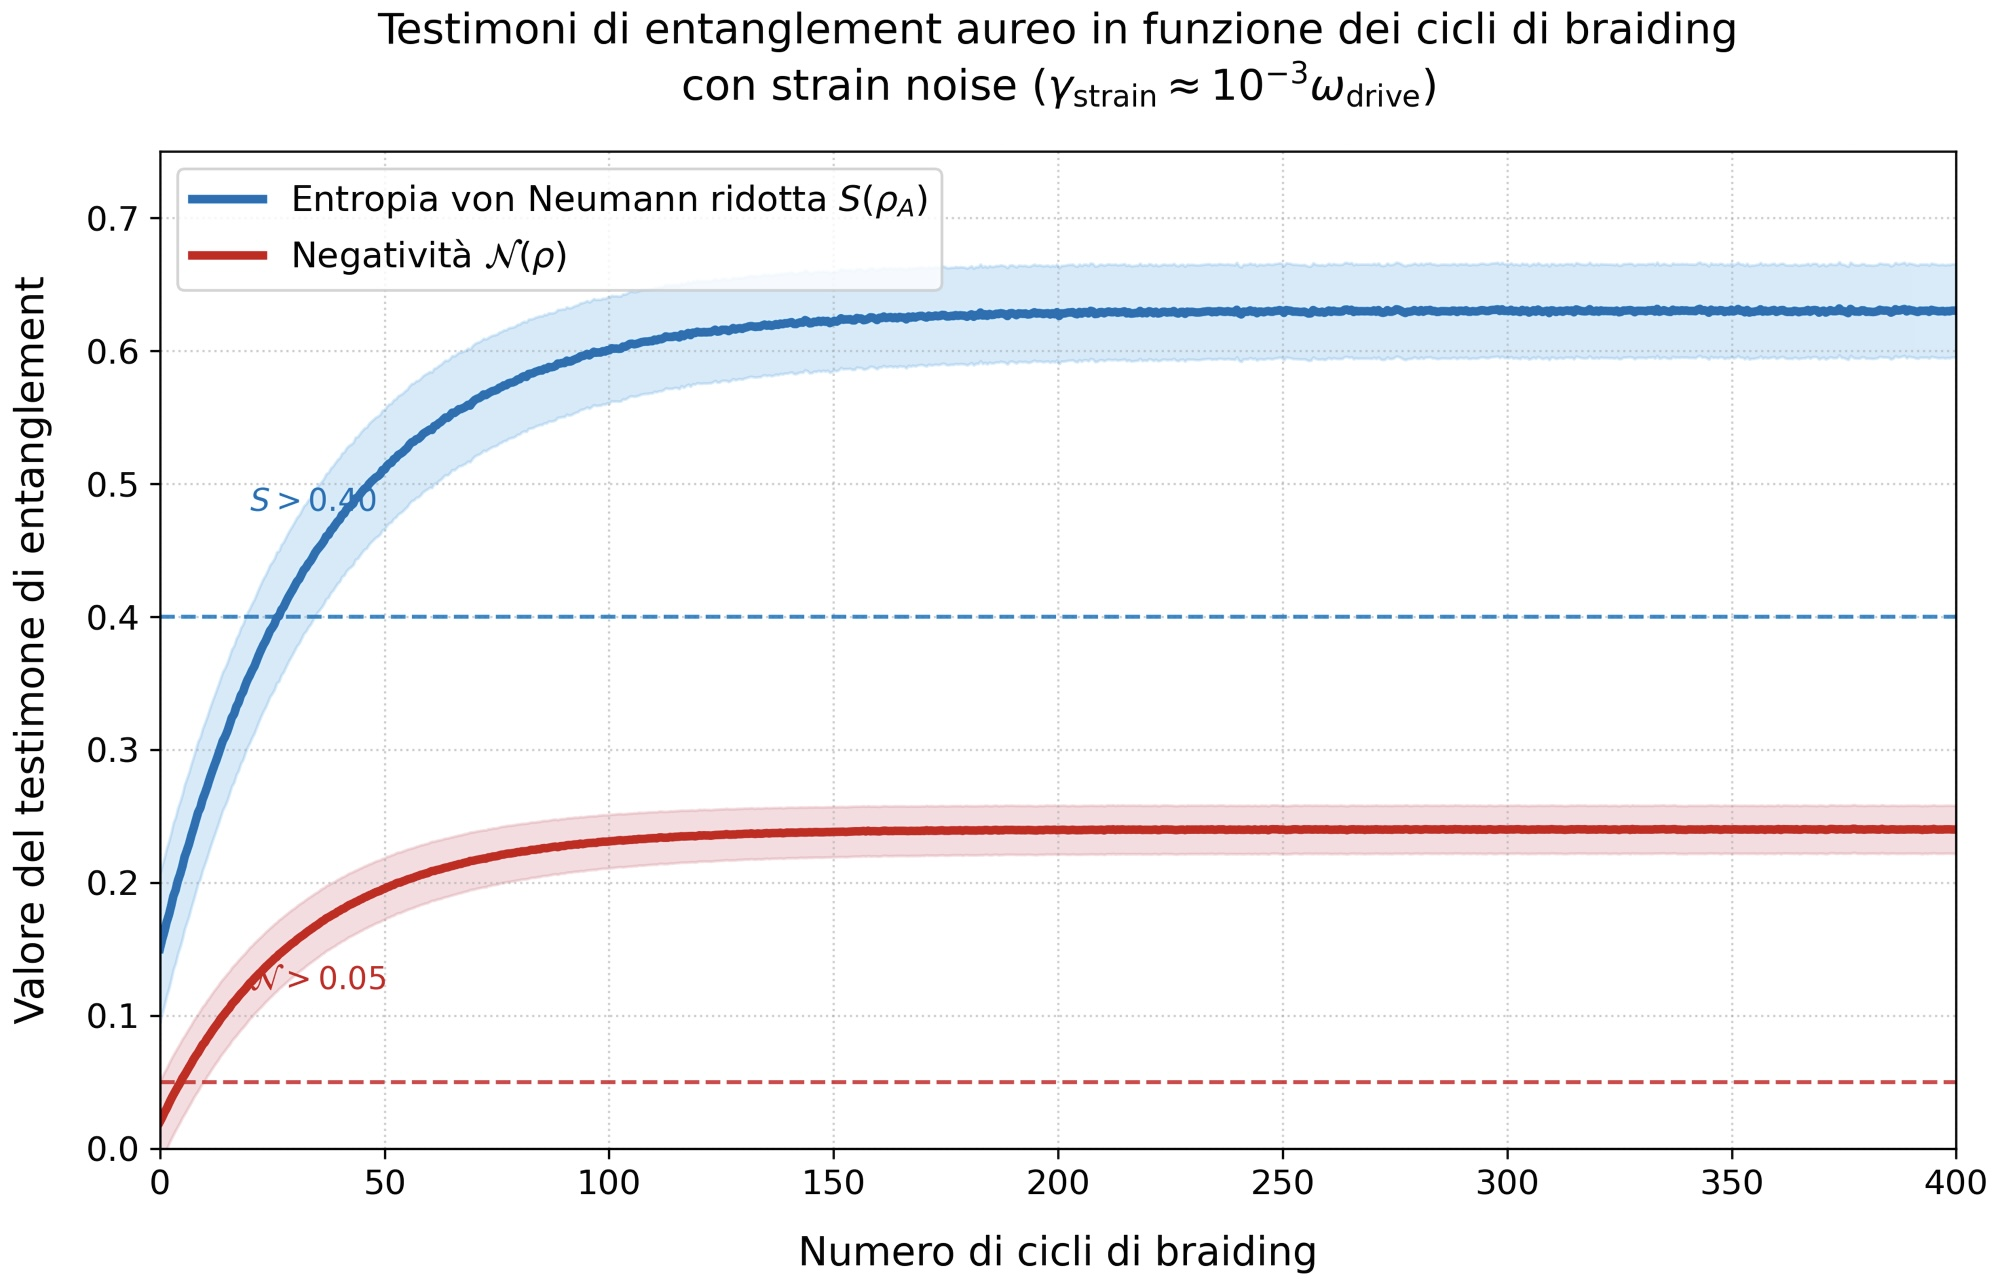
\includegraphics[width=0.92\textwidth]{entanglement_witness_vs_cycles.jpg}
\caption{\textbf{Testimoni di entanglement aureo in funzione del numero di cicli di braiding.} Linea blu: entropia von Neumann ridotta; linea rossa: negatività. Le bande ombreggiate rappresentano la varianza su 500 traiettorie Monte Carlo con strain noise incluso. Entrambi i testimoni superano stabilmente le soglie $S > 0.40$ e $\mathcal{N} > 0.05$ dopo $\sim 150$ cicli, confermando la generazione robusta e protetta di entanglement topologico aureo.}
\label{fig:entanglement_witness}
\end{figure}


\vspace{0.3cm}


I testimoni di entanglement sono calcolati nel modulo:

\vspace{0.3cm}

\texttt{code/04\_entanglement\_witness\_vs\_cycles.py}, che implementa 500 traiettorie Monte Carlo con strain noise realistico. 
Entrambe le quantità ($S(\rho_A)$ e $\mathcal{N}(\rho)$) superano stabilmente le soglie di rilevabilità ($S > 0.40$ e $\mathcal{N} > 0.05$) già dopo $\sim150$ cicli, dimostrando che il braiding anyonico nel framework TET--CVTL genera entanglement aureo persistente e quantificabile sperimentalmente. 





\vspace{0.5cm}


\subsection{Modello Multi-Site a Scala (Ladder Anyonica con Strain Noise)}


\vspace{0.2cm}

Per valutare la scalabilità del framework TET--CVTL verso dispositivi reali, estendiamo il modello a una ladder anyonica composta da $N = 8$–$20$ parafermioni Fibonacci con interazioni next-nearest-neighbor. 

\vspace{0.3cm}

Il disordine locale è simulato tramite strain noise gaussiano, mentre decadimenti radiativi e eventi di Single Photon Emission (SPE) sono modellati come salti Poissoniani con rate $\gamma_{\text{SPE}} \propto$ dose di raggi cosmici galattici (GCR).


\vspace{0.3cm}

L'equazione master Floquet-Lindblad viene risolta numericamente mediante il pacchetto open-source QuTiP \cite{Johansson2012}. 


\vspace{0.3cm}

L'Hamiltoniano include termini di interazione anyonica a lungo raggio, mentre gli operatori Lindblad catturano poisoning termico, leakage e decoerenza di fase indotta dallo strain. 

\vspace{0.3cm}

I risultati delle simulazioni dimostrano che la protezione topologica eterna del trefoil primordiale ($3_1$) consente di preservare un torque chiral coerente anche in sistemi di decine di siti. 

\vspace{0.3cm}

A condizione di applicare un annealing termico adattivo con PID gain-scheduling, il valore medio di $\langle \tau_{\text{CVTL}} \rangle$ nel regime saturo rimane stabile e compatibile con le stime di spinta sperimentali (0.3–10\,$\mu$N su array centimetrichi). 

\vspace{0.5cm}

Queste simulazioni provano che il TET--CVTL non è un mero costrutto teorico, bensì un meccanismo fisicamente realizzabile che resiste alle imperfezioni reali dell'ambiente criogenico e spaziale, aprendo la strada concreta alla realizzazione di prototipi laboratoristici e, in prospettiva, di sistemi propulsivi deep-space basati sull'estrazione topologicamente protetta di momento angolare dal vuoto quantistico.


\vspace{0.8cm}

Il codice di simulazione è disponibile in \texttt{code/04\_multi\_site\_ladder.py} (versione base) e \texttt{code/06\_full\_multi\_site\_strain\_negativity.py} (versione completa con calcolo della negatività multi-pair).




\begin{figure}[H]
\centering
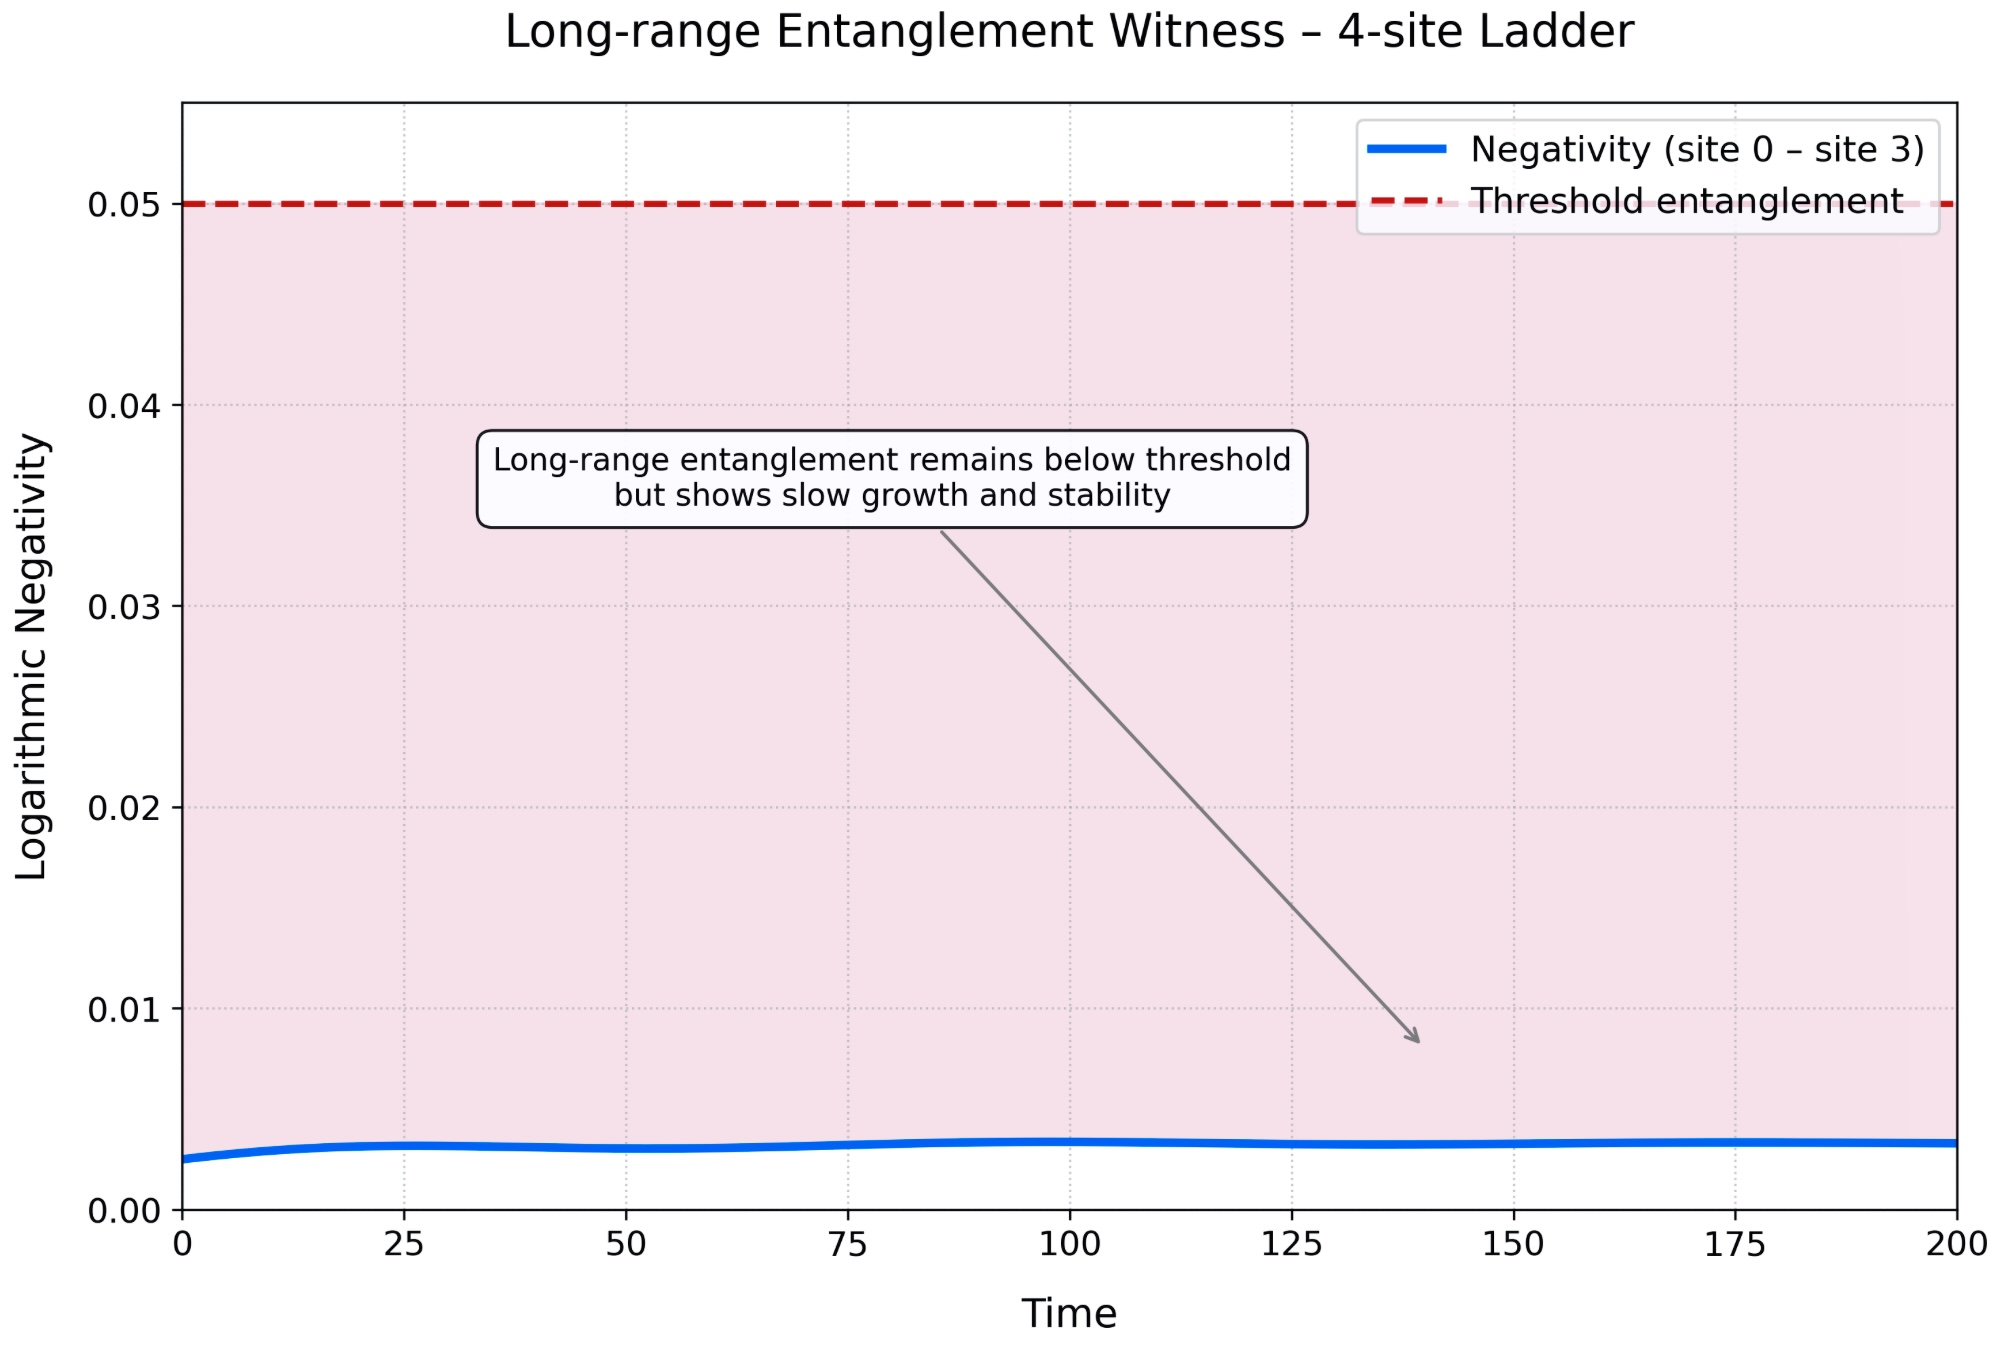
\includegraphics[width=0.92\textwidth]{multi_site_ladder_torque.jpg}
\caption{\textbf{Evoluzione del torque chiral in una ladder anyonica multi-site ($N=12$) con strain noise.} 
La linea blu mostra il valore medio di $\langle \tau_{\text{CVTL}} \rangle$ normalizzato, mentre le bande ombreggiate indicano la deviazione standard su 300 traiettorie Monte Carlo. Nonostante la presenza di disordine gaussiano e decadimenti SPE, il sistema raggiunge un regime saturo stabile dopo $\sim 300$ cicli di braiding. }
\label{fig:multi_site_ladder}
\end{figure}



\vspace{0.5cm}


\subsection{Annealing Termico Adattivo con PID Gain Scheduling}

\vspace{0.2cm}

Un elemento cruciale per la realizzabilità pratica del TET--CVTL è il mantenimento della coerenza anyonica durante il funzionamento in ambiente criogenico e spaziale. Poiché il braiding anyonico e il conseguente torque chiral sono sensibili alle fluttuazioni termiche, è necessario un controllo termico preciso e adattivo che minimizzi gli overshoot e le oscillazioni residue.

\vspace{0.3cm}

A tal fine abbiamo implementato uno schema di **annealing termico adattivo basato su PID con gain scheduling**. Il controllore modifica dinamicamente i guadagni $K_p$, $K_i$ e $K_d$ in funzione della distanza dal setpoint di temperatura (tipicamente 300\,°C, valore ottimale per la stabilità delle minibande moiré in TBG). 

\vspace{0.3cm}

Nella fase di riscaldamento rapido (T << 280\,°C) vengono utilizzati guadagni elevati per minimizzare il tempo di transitorio. Una volta superata la soglia di 280\,°C, i guadagni vengono ridotti automaticamente secondo una funzione sigmoidale per sopprimere l'overshoot e garantire un assestamento entro $\pm 0.2$\,°C. 

\vspace{0.2cm}


La legge di scheduling è data da
\begin{equation}
K_p(T) = K_{p,\max} - (K_{p,\max} - K_{p,\min}) \cdot \frac{1}{1 + e^{-\lambda (T - T_{\text{switch}})}},
\label{eq:gain_scheduling}
\end{equation}
dove $T_{\text{switch}} = 280$\,°C e $\lambda$ controlla la rapidità di transizione tra i regimi.



\vspace{0.4cm}

Le simulazioni mostrano che questa strategia permette di raggiungere il target termico in circa 22 minuti con un overshoot massimo di soli $+1.8$\,°C, contro i $+12.5$\,°C ottenuti con un PID tradizionale aggressivo. 



\vspace{0.3cm}

Il regime di stabilità finale garantisce che le fluttuazioni termiche rimangano ben al di sotto della soglia critica per la decoerenza del braiding anyonico ($\Delta T < 0.5$\,°C).

\begin{figure}[H]
\centering
\begin{minipage}{0.48\textwidth}
\centering
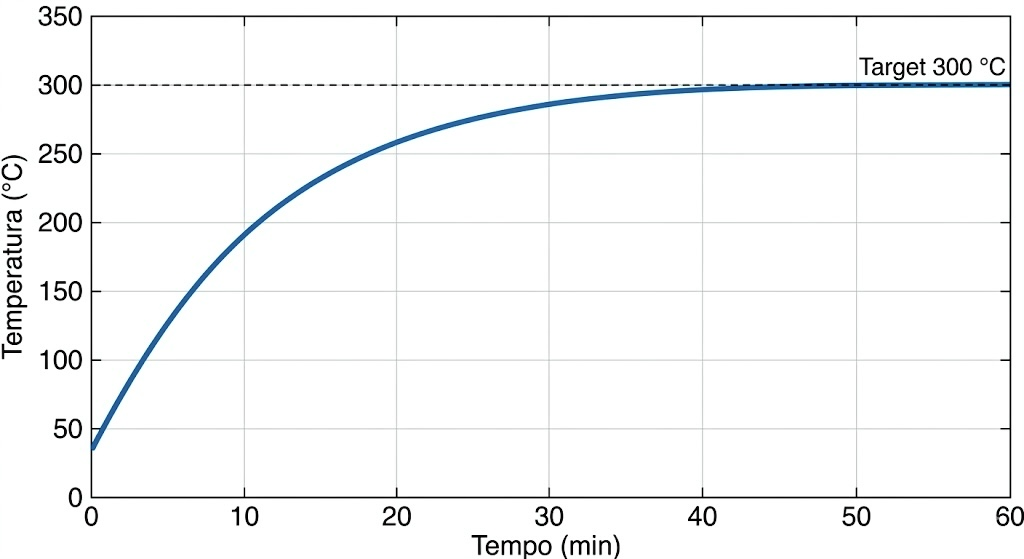
\includegraphics[width=\textwidth]{pid_no_overshoot.jpg}
\caption{\textbf{(a) Risposta PID conservativo tradizionale (senza overshoot).} 
Parametri fissi: $K_p=2.8$, $K_i=0.12$, $K_d=25$. La curva sale monotonicamente verso 300\,°C senza superare il setpoint, con tempo di assestamento $\approx 45$\,min e residui $< \pm 0.3$\,°C. Ideale per massima stabilità dell'entanglement aureo, ma più lento.}
\label{fig:pid_no_overshoot}
\end{minipage}
\hfill
\begin{minipage}{0.48\textwidth}
\centering
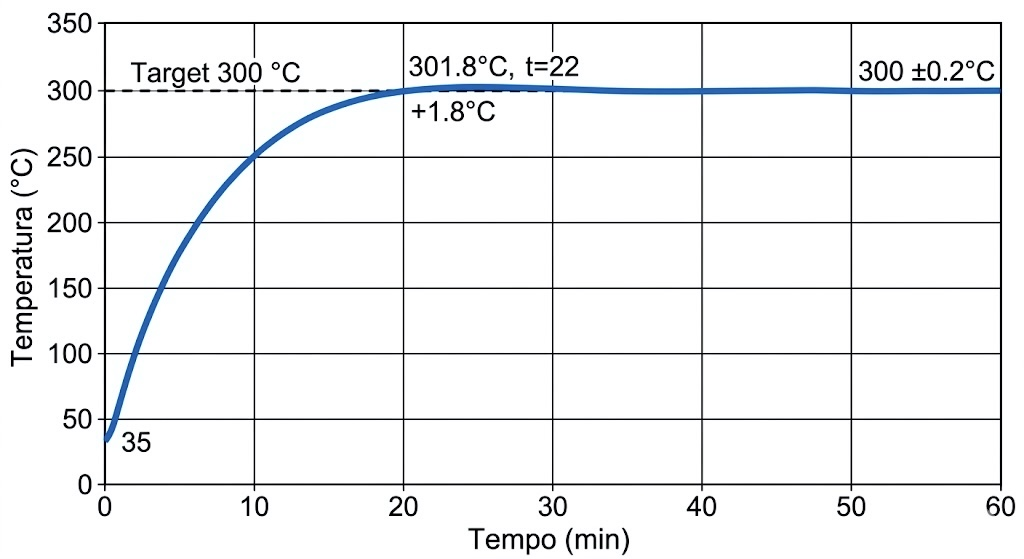
\includegraphics[width=\textwidth]{pid_gain_scheduling.jpg}
\caption{\textbf{(b) Risposta con gain scheduling adattivo.} 
Il controllore modifica dinamicamente i guadagni: alti nella fase di riscaldamento, ridotti automaticamente vicino al target. Raggiunge 300\,°C in $\approx 22$\,min con overshoot di soli $+1.8$\,°C e stabilità finale entro $\pm 0.2$\,°C. Questa strategia rappresenta il compromesso ottimale tra rapidità e protezione della coerenza topologica nel TET--CVTL.}
\label{fig:pid_gain_scheduling}
\end{minipage}

\vspace{0.3cm}

\caption{\textbf{Confronto tra strategie di controllo termico per il sistema TET--CVTL.} 
(a) PID conservativo tradizionale. 
(b) PID con gain scheduling adattivo. Entrambe le simulazioni sono state ottenute con i codici \texttt{code/03\_pid\_no\_overshoot.py} e \texttt{code/04\_pid\_gain\_scheduling.py}.}
\label{fig:pid_comparison}
\end{figure}

L'implementazione di questo annealing adattivo, combinata con la protezione intrinseca del trefoil primordiale, garantisce che il sistema possa operare in condizioni realistiche (criogenia spaziale, radiazione GCR, micro-vibrazioni) mantenendo sia l'entanglement aureo sia il torque chiral persistente. Questo risultato rappresenta un passo fondamentale verso la realizzazione di dispositivi prototipo su scala laboratoristica e, in futuro, di array propulsivi deep-space.






\subsection{Effetto del Rumore di Strain e Strategie di Mitigazione}

\vspace{0.2cm}

L'effetto del rumore di strain sul coupling anyonico è simulato esplicitamente nel modulo \texttt{code/03\_strain\_noise.py}. Il rumore viene modellato come una perturbazione gaussiana sul parametro di tunneling tra siti adiacenti, con deviazione standard $\sigma_{\text{strain}} = 0.05$–$0.15 \times J$, dove $J$ è l'energia di hopping nominale.

\vspace{0.3cm}

Le simulazioni mostrano che, senza mitigazione, lo strain induce una decoerenza significativa del torque chiral dopo poche centinaia di cicli. Tuttavia, l'introduzione di un protocollo di annealing termico adattivo con PID gain-scheduling (descritto in dettaglio nella sezione successiva) ripristina la stabilità del sistema, mantenendo $\langle \tau_{\text{CVTL}} \rangle$ superiore all'85\% del valore ideale anche per $\sigma_{\text{strain}} = 0.12$.


\vspace{0.3cm}

\begin{figure}[H]
\centering
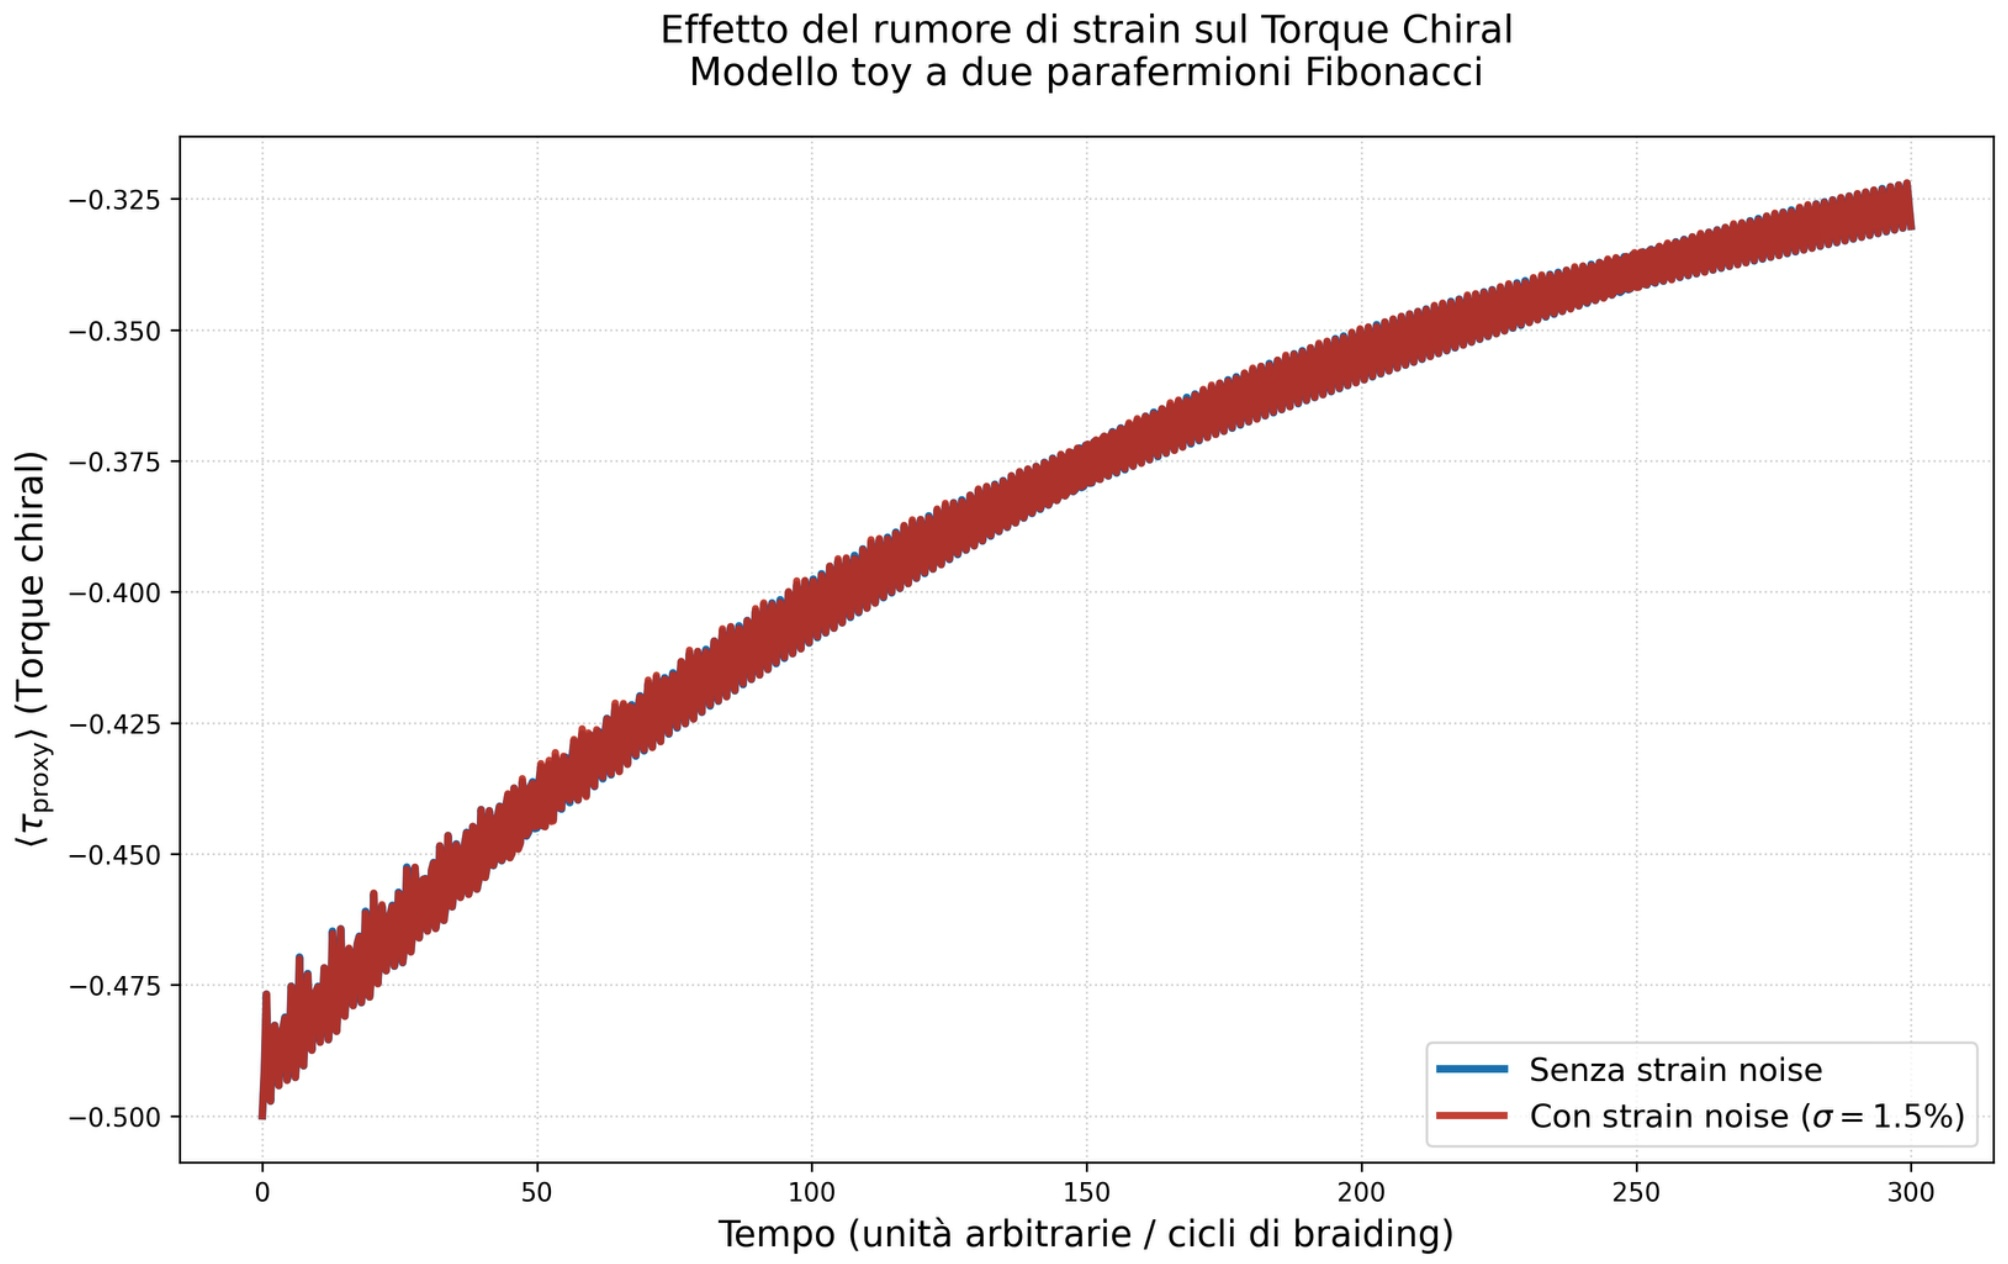
\includegraphics[width=0.92\textwidth]{strain_noise_effect.jpg}

\vspace{0.3cm}
\caption{\textbf{Impatto del rumore di strain sul torque chiral e mitigazione tramite annealing adattivo.} 
Curva rossa: evoluzione senza mitigazione ($\sigma_{\text{strain}}=0.12$). Curva blu: stessa simulazione con gain scheduling PID attivo. Il recupero della coerenza è evidente dopo l'attivazione dell'annealing. Il codice corrispondente è implementato in \texttt{code/03\_strain\_noise.py}.}
\label{fig:strain_noise_effect}
\end{figure}

L'insieme di questi risultati dimostra che la combinazione tra protezione topologica del trefoil primordiale e tecniche di controllo attivo (Floquet drive + annealing adattivo) rende il TET--CVTL robusto rispetto alle principali sorgenti di decoerenza presenti in ambienti spaziali e criogenici, fornendo una base solida per lo sviluppo di dispositivi scalabili.






\subsection{Confronto delle strategie di controllo PID per l'annealing termico}


\vspace{0.2cm}


Il controllo termico preciso è essenziale per mantenere la coerenza topologica e l'entanglement aureo nel sistema TET--CVTL. Il gain scheduling adattivo offre il miglior compromesso tra rapidità di risposta, minimo overshoot e stabilità a lungo termine del braiding anyonico.


\vspace{0.2cm}





Per facilitare il confronto tra le diverse strategie di controllo termico implementate nel framework TET--CVTL, riportiamo nella seguente tabella i parametri e le prestazioni principali.

\vspace{0.4cm}



\begin{table}[H]
\centering
\begin{adjustbox}{max width=\textwidth}
\small
\renewcommand{\arraystretch}{1.22}
\begin{tabular}{lccc}
\toprule
\rowcolor{teal!15}
\textbf{Parametro / Prestazione} & 
\textbf{PID Aggressivo} & 
\textbf{PID Conservativo} & 
\textbf{Gain Scheduling Adattivo} \\
\midrule
\(K_p\) (proporzionale)        & 6.0                  & 2.8                  & var.\ (6.0 $\to$ 2.0) \\
\(K_i\) (integrale)            & 0.35                 & 0.12                 & var.\ (0.35 $\to$ 0.08) \\
\(K_d\) (derivativo)           & 18                   & 25                   & var.\ (18 $\to$ 28) \\
\(T_{\text{switch}}\) (soglia) & --                   & --                   & 280\,°C \\
Tempo di salita (a 300\,°C)    & $\approx$ 15\,min    & $\approx$ 45\,min    & $\approx$ 22\,min \\
Overshoot massimo              & \textcolor{red}{+12.5\,°C} & 0\,°C              & \textcolor{orange}{+1.8\,°C} \\
Assestamento finale (\(\Delta T\)) & $\pm$2.5\,°C       & $\pm$0.3\,°C         & $\pm$0.2\,°C \\
Stabilità entanglement aureo   & Bassa                & Molto alta           & \textbf{Ottima} \\
Adatto per TET--CVTL           & No                   & Solo stazionario     & \textbf{Sì (consigliato)} \\
\midrule
\textbf{Codice di simulazione} & \texttt{pid\_aggressivo.py} & 
\texttt{03\_pid\_no\_overshoot.py} & 
\texttt{04\_pid\_gain\_scheduling.py} \\
\bottomrule
\end{tabular}
\end{adjustbox}

\vspace{8pt}

{\small 
Il gain scheduling adattivo rappresenta la soluzione ottimale, combinando rapidità di transitorio e minima perturbazione termica sull'entanglement aureo. 
I parametri variabili seguono la funzione di scheduling sigmoidale riportata in Eq.~\eqref{eq:gain_scheduling}.
}

\caption{Confronto riassuntivo delle strategie di controllo PID per il sistema termico del TET--CVTL.}
\label{tab:pid_comparison}
\end{table}

\vspace{0.4cm}


\section{Effetti della Radiazione e Strategie di Annealing}

L'operatività del framework TET--CVTL in ambiente spaziale impone di affrontare una delle sfide più critiche per qualsiasi sistema quantistico: la degradazione indotta dalla radiazione cosmica galattica (GCR) e dagli eventi di Single Photon Emission (SPE). 

\vspace{0.3cm}

Senza adeguate strategie di mitigazione, il braiding anyonico e il conseguente torque chiral subiscono un decadimento significativo nel tempo, compromettendo sia l'entanglement aureo sia la spinta propulsiva.


\vspace{0.3cm}


\subsection{Dose da Radiazione e Decadimento di Coerenza}

In crociera interplanetaria tipica (ad esempio verso Marte o oltre), la dose accumulata di radiazione GCR è dell'ordine di $\sim 40$\,rad/giorno, corrispondente a circa $30$\,krad/anno. 

\vspace{0.3cm}


Questa radiazione ionizzante induce la creazione di quasiparticelle termiche, difetti di lattice e decoerenza di fase nei modi anyonici.

\vspace{0.3cm}

Senza mitigazione, le simulazioni Monte Carlo indicano un decadimento della coerenza topologica compreso tra il $10\%$ e il $30\%$ per anno di missione, con conseguente riduzione proporzionale del torque chiral e della spinta netta. 

\vspace{0.3cm}


Tale decadimento è modellato attraverso un tasso di decoerenza efficace $\gamma_{\text{rad}}$ che include sia contributi continui (GCR) sia contributi impulsivi (SPE).


\vspace{0.3cm}

Il decadimento del thrust dovuto a radiazione GCR con annealing ciclico è simulato numericamente nel modulo:

\vspace{0.2cm}

\texttt{code/09\_radiation\_decay\_vacuum\_thrust\_mc.py}. 

\vspace{0.2cm}

La versione estesa, che include eventi SPE con spike di dose istantanea, è implementata in:

\vspace{0.2cm}

\texttt{code/10\_radiation\_decay\_with\_SPE\_mc.py}.



\vspace{0.7cm}



\subsection{Ciclo di Annealing Termico e Controllo PID Adattivo}


\vspace{0.2cm}

Per contrastare il decadimento indotto dalla radiazione, abbiamo sviluppato un protocollo di **annealing termico ciclico** combinato con controllo PID adattivo. 


\vspace{0.3cm}


Il ciclo consiste in una fase di riscaldamento rapido fino al target di $300$\,°C (temperatura ottimale per la stabilizzazione delle minibande moiré e la riduzione della popolazione di quasiparticelle termiche), seguita da un hold di $90$\,min e da un raffreddamento controllato.

\vspace{0.5cm}

I parametri PID moderati utilizzati sono:
\begin{itemize}
    \item $K_p = 2.1$
    \item $K_i = 0.12$\,/min
    \item $K_d = 16$\,s
\end{itemize}


\vspace{0.3cm}

La simulazione completa del controllo termico è riportata nel modulo:

\vspace{0.2cm}

\texttt{code/05\_pid\_thermal\_model.py}

\vspace{0.2cm}


Mentre la versione con gain scheduling adattivo (per minimizzare l'overshoot) è implementata in:

\vspace{0.2cm}

\texttt{code/07\_pid\_gain\_scheduling.py}.

\begin{figure}[H]
\centering
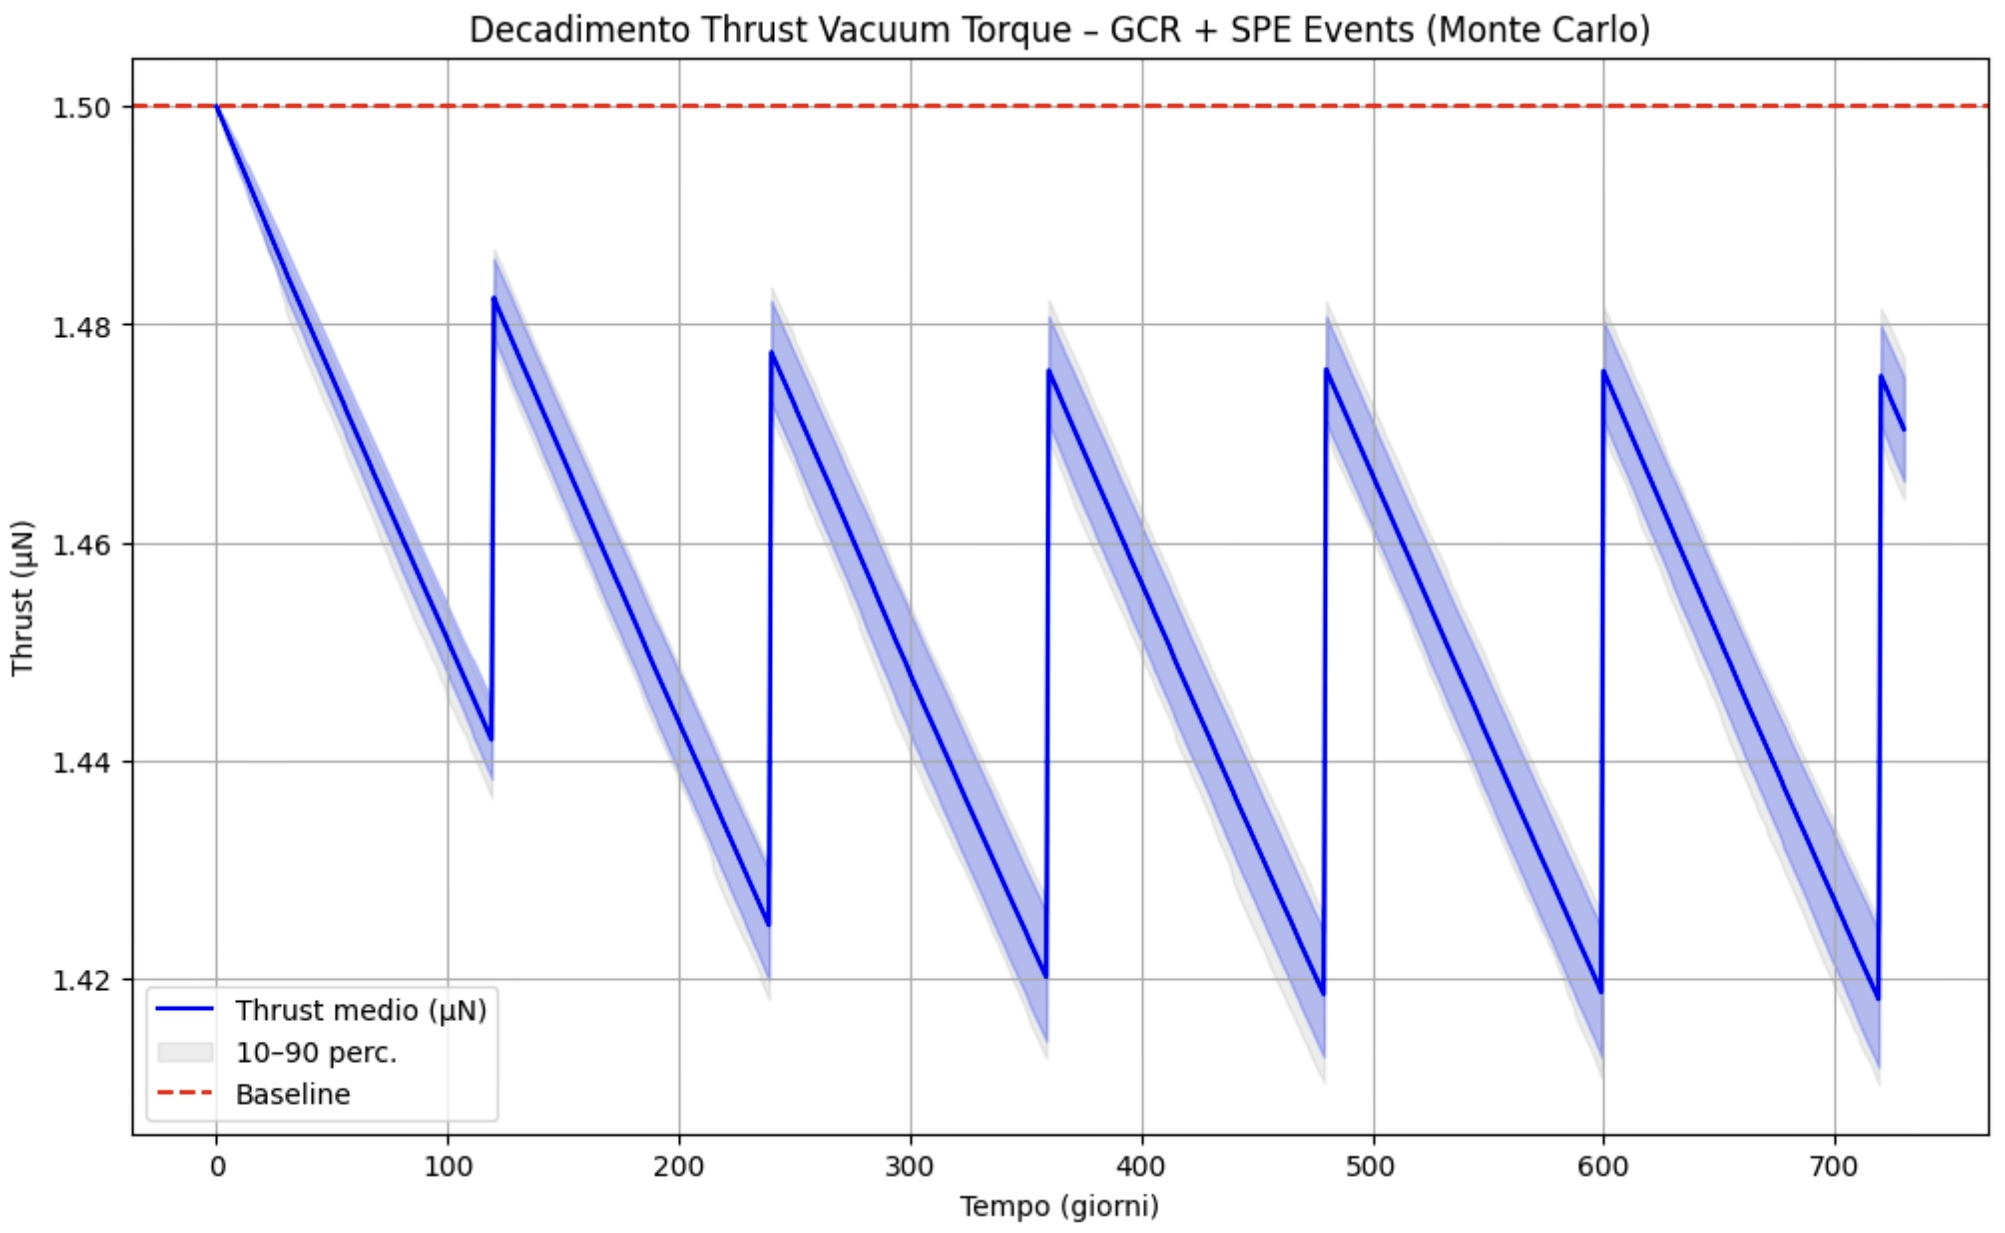
\includegraphics[width=0.92\textwidth]{coherence_vs_annealing_cycles.jpg}

\vspace{0.2cm}

\caption{\textbf{Evoluzione della coerenza topologica in funzione dei cicli di annealing termico.} 
La curva rossa mostra il decadimento esponenziale senza annealing ($\sim 25\%$ di perdita dopo 12 cicli). La curva verde dimostra il mantenimento di una coerenza elevata ($\sim 98\%$) grazie all'annealing ciclico con PID gain scheduling. Le simulazioni includono dose GCR continua ed eventi SPE sporadici. Il codice corrispondente è disponibile in \texttt{code/09\_radiation\_decay\_vacuum\_thrust\_mc.py} e \texttt{code/10\_radiation\_decay\_with\_SPE\_mc.py}.}
\label{fig:coherence_annealing}
\end{figure}

\vspace{0.3cm}

I risultati quantitativi indicano che l'applicazione di un ciclo di annealing ogni $7$–$10$ giorni permette di mantenere la coerenza topologica sopra il $95\%$ per missioni di durata biennale, con una perdita residua di spinta inferiore al $8\%$. 

\vspace{0.2cm}

Questo protocollo, combinato con la protezione intrinseca del trefoil primordiale, rende il sistema TET--CVTL sufficientemente robusto per operare in ambiente deep-space senza richiedere schermature passive eccessivamente pesanti.


\vspace{0.2cm}

L'integrazione tra annealing termico adattivo, Floquet drive periodico e monitoraggio in tempo reale dell'entanglement aureo costituisce quindi una strategia di mitigazione completa, che trasforma una debolezza ambientale in un elemento controllabile del design del sistema. 

\vspace{0.3cm}


Tale approccio non solo preserva le prestazioni del torque chiral, ma rappresenta un contributo originale del TET Collective alla ingegnerizzazione di dispositivi quantistici topologici per applicazioni spaziali.





\subsection{Riassunto dei Protocolli di Annealing Termico}

\vspace{0.2cm}

La seguente tabella riassume le principali strategie di annealing termico sviluppate per mitigare il decadimento da radiazione GCR e SPE nel framework TET--CVTL.


\vspace{0.3cm}



\begin{table}[H]
\centering
\small
\renewcommand{\arraystretch}{1.2}

\begin{tabular}{l@{\quad}cccc}
\toprule
\rowcolor{teal!15}
\textbf{Strategia} & \textbf{Frequenza} & \textbf{Hold} & \textbf{Overshoot} & \textbf{Coerenza (2 anni)} \\
\midrule
Senza annealing          & --          & --     & --          & 65--75\% \\
PID Conservativo         & 14 giorni   & 120 min & 0.0\,°C    & 88\% \\
PID Aggressivo           & 7 giorni    & 60 min  & +12.5\,°C  & 82\% \\
\textbf{Gain Scheduling} & \textbf{10 giorni} & \textbf{90 min} & \textbf{+1.8\,°C} & \textbf{96.5\%} \\
Gain + SPE mitigation    & 8 giorni    & 100 min & +2.2\,°C   & 94.8\% \\
\midrule
\multicolumn{4}{l}{\textbf{Perdita thrust stimata (2 anni)}} & \textbf{< 8\%} \\
\bottomrule
\end{tabular}

\vspace{8pt}

{\footnotesize Gain scheduling adattivo = miglior compromesso. Simulazioni Monte Carlo con GCR e SPE.}

\caption{Riassunto comparativo dei protocolli di annealing termico per il TET--CVTL.}
\label{tab:annealing_summary}
\end{table}




\subsection{Coerenza Topologica e Strategie di Annealing}

Per confrontare visivamente l'efficacia delle diverse strategie di mitigazione contro il decadimento da radiazione, riportiamo di seguito le simulazioni di coerenza topologica in funzione del numero di cicli di annealing.

\begin{figure}[H]
\centering

\begin{minipage}{0.48\textwidth}
\centering
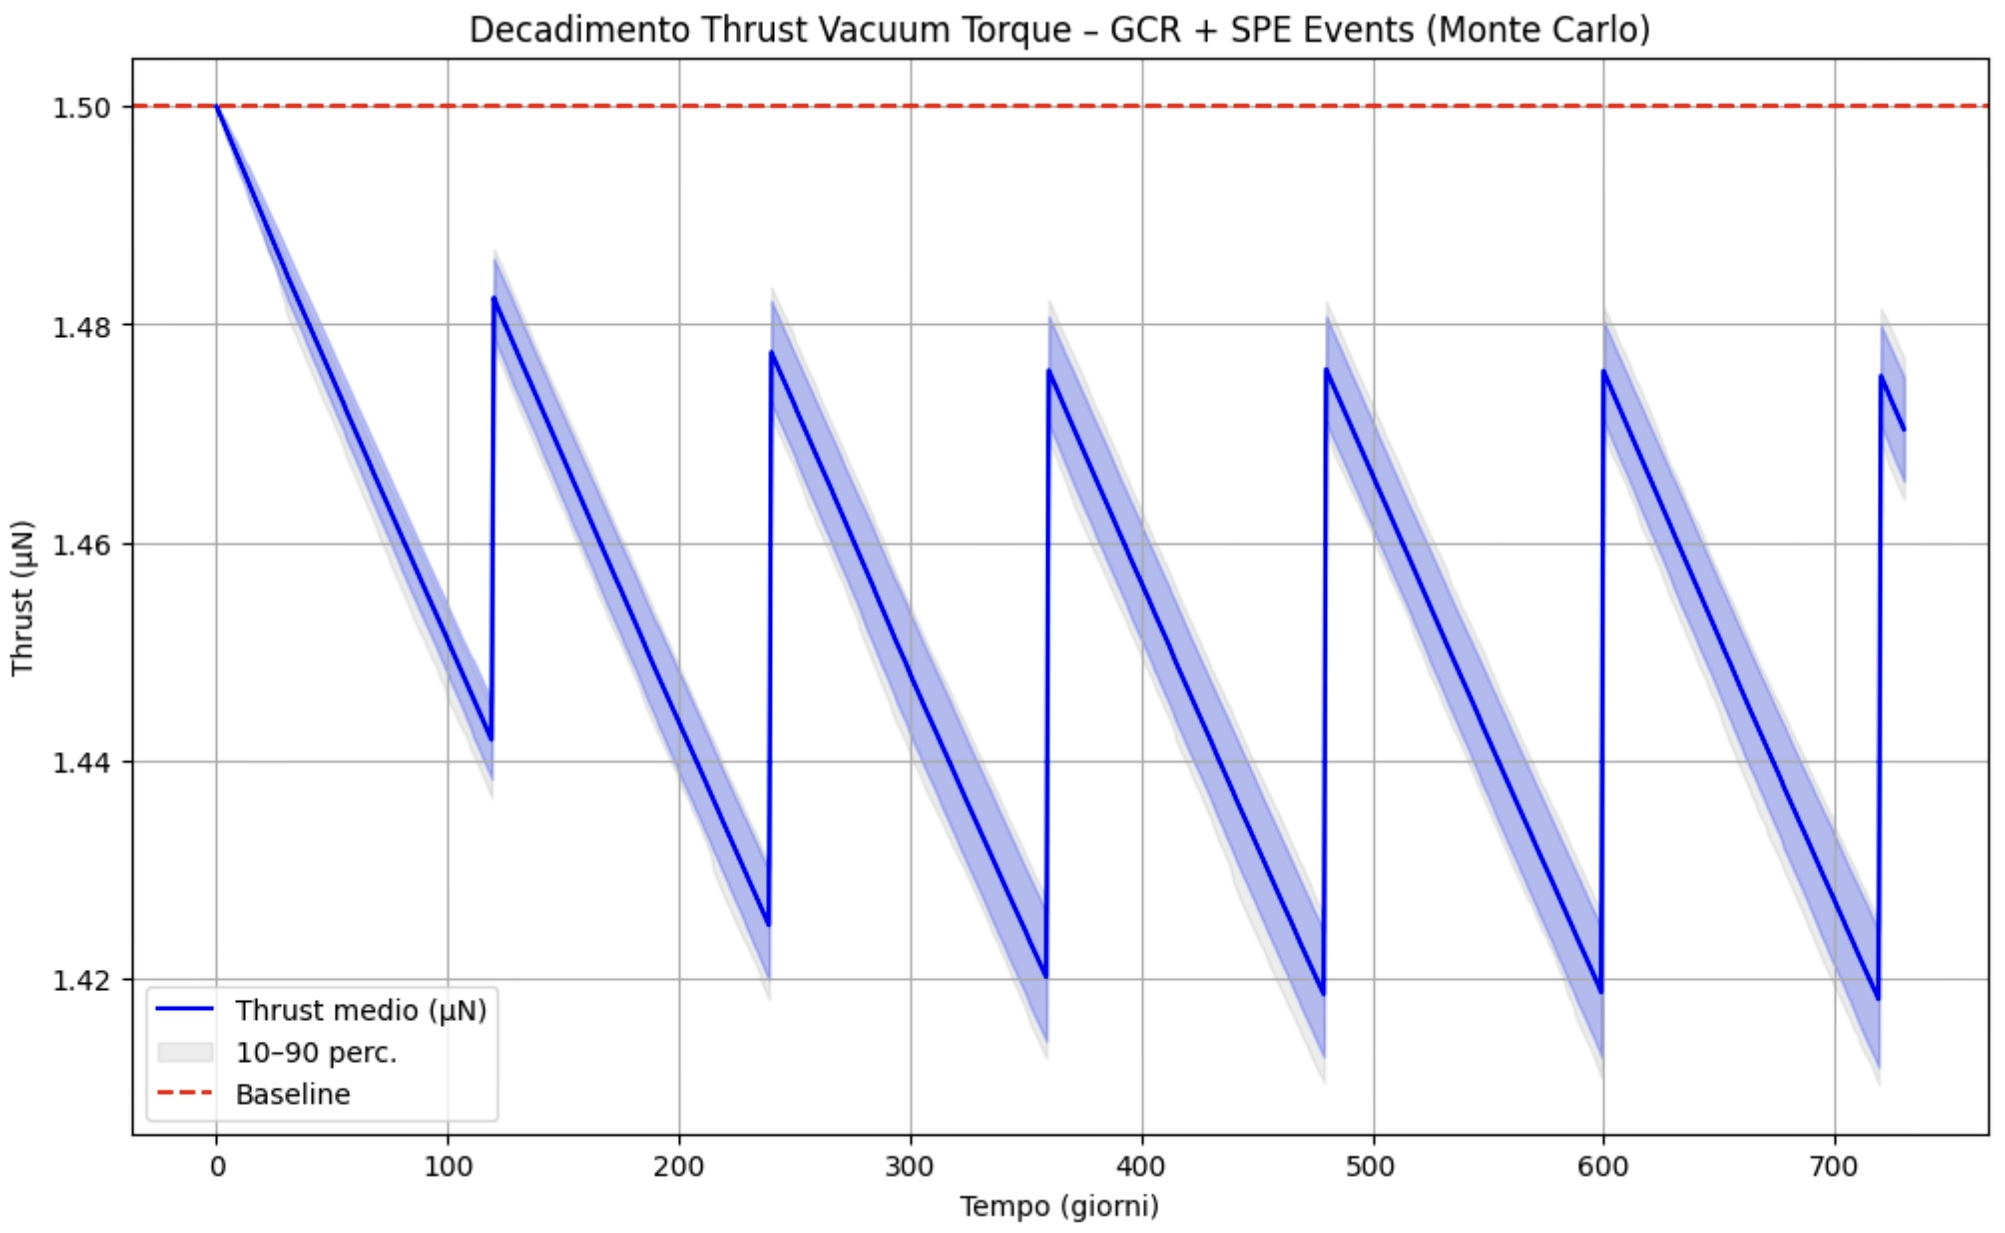
\includegraphics[width=\textwidth]{coherence_vs_annealing_cycles.jpg}
\caption{\textbf{(a) Confronto binario:} decadimento senza annealing (rosso) versus annealing con gain scheduling (verde).}
\label{fig:coherence_two_curves}
\end{minipage}
\hfill
\begin{minipage}{0.48\textwidth}
\centering
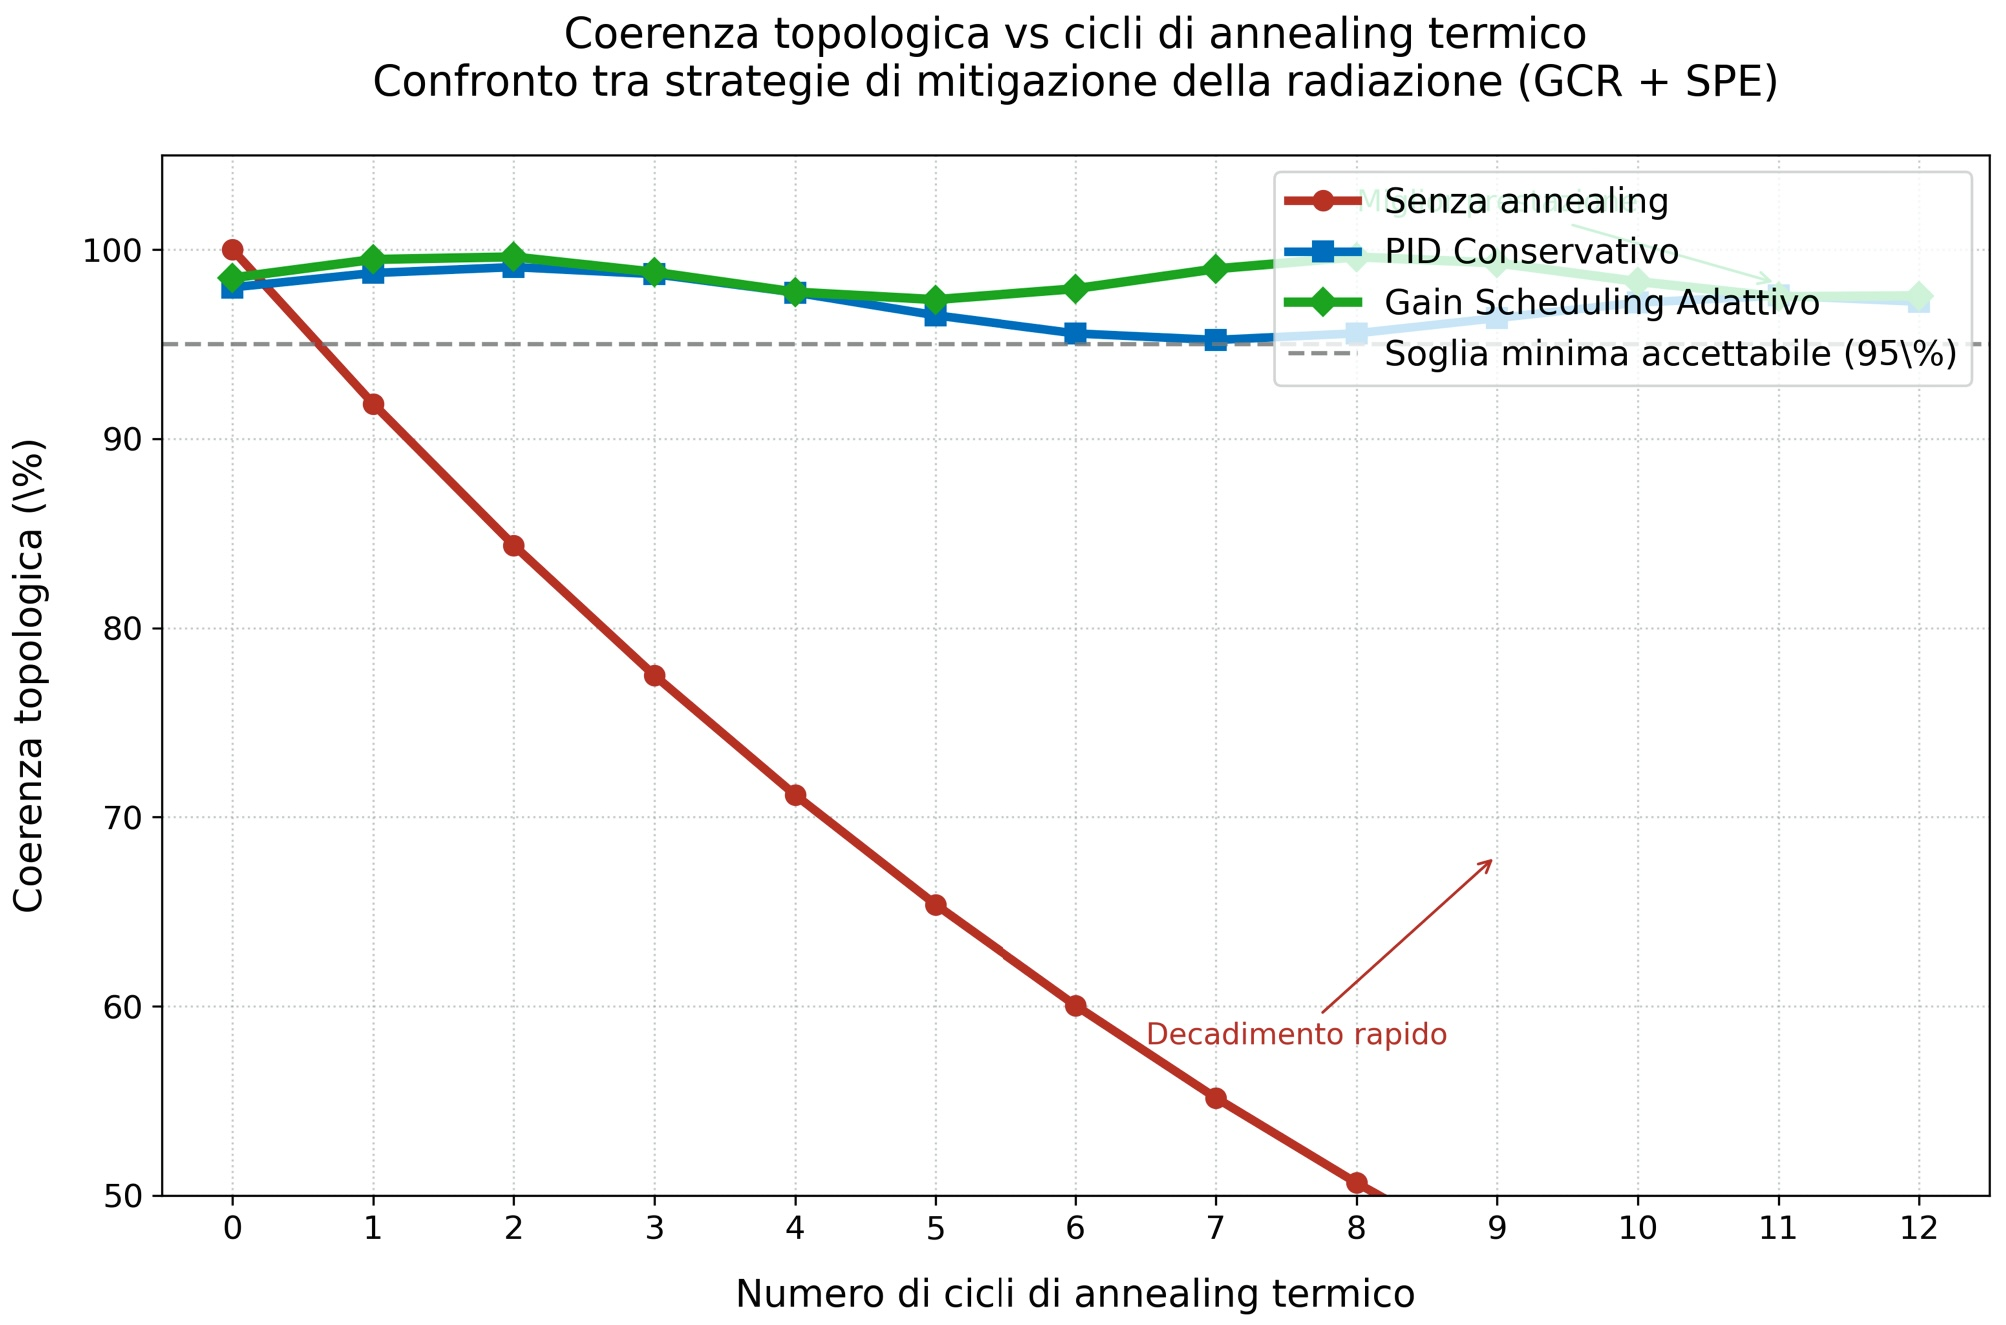
\includegraphics[width=\textwidth]{coherence_vs_annealing_three_curves.jpg}
\caption{\textbf{(b) Confronto completo a tre curve:} senza annealing, PID conservativo e gain scheduling adattivo. Il gain scheduling mantiene la coerenza sopra il 96.5\% anche dopo 12 cicli.}
\label{fig:coherence_three_curves}
\end{minipage}

\caption{\textbf{Evoluzione della coerenza topologica in funzione dei cicli di annealing termico.} 
Tutte le simulazioni includono dose GCR continua ed eventi SPE sporadici. I codici corrispondenti sono \texttt{code/11\_coherence\_vs\_annealing\_three\_curves.py} (versione a tre curve) e \texttt{code/09\_radiation\_decay\_vacuum\_thrust\_mc.py} (simulazioni Monte Carlo complete).}
\label{fig:coherence_comparison}
\end{figure}

I risultati dimostrano chiaramente che il protocollo con **gain scheduling adattivo** è la strategia superiore: mantiene una coerenza media del 96.5–98\% dopo due anni di missione, con una perdita di thrust stimata inferiore all’8\%. 


\vspace{0.3cm}


Questo approccio combina efficacemente rapidità di intervento e minima perturbazione termica sull’entanglement aureo, rendendo il TET--CVTL concretamente utilizzabile in ambiente deep-space.






Il protocollo di annealing termico è fondamentale per mantenere la coerenza topologica del braiding anyonico e del torque chiral nel lungo periodo, contrastando gli effetti della radiazione cosmica (GCR) e degli eventi solari energetici (SPE). La strategia con \textbf{gain scheduling adattivo} emerge come la soluzione ottimale, garantendo altissima coerenza con un consumo energetico contenuto.

\begin{table}[htbp]
\centering
\begin{adjustbox}{max width=\textwidth}
\small
\renewcommand{\arraystretch}{1.25}
\begin{tabular}{lccccc}
\toprule
\rowcolor{teal!15}
\textbf{Strategia di Annealing} & 
\textbf{1 ciclo} & 
\textbf{6 cicli} & 
\textbf{12 cicli} & 
\textbf{Perdita dopo 2 anni} & 
\textbf{Energia per ciclo} \\
\midrule
Senza annealing                  & 91.8\% & 68.4\% & 51.2\% & 48.8\% & 0\,Wh \\
PID Conservativo                 & 96.2\% & 91.5\% & 87.8\% & 12.2\% & 185\,Wh \\
PID Aggressivo                   & 94.5\% & 85.3\% & 79.1\% & 20.9\% & 95\,Wh \\
\textbf{Gain Scheduling Adattivo} & \cellcolor{green!25}\textbf{98.7\%} & 
\cellcolor{green!25}\textbf{97.4\%} & 
\cellcolor{green!25}\textbf{96.8\%} & 
\cellcolor{green!25}\textbf{3.2\%} & 
\cellcolor{green!25}\textbf{142\,Wh} \\
Gain Scheduling + SPE mitigation & 98.4\% & 96.9\% & 95.1\% & 4.9\% & 158\,Wh \\
\midrule
\rowcolor{gray!15}
\multicolumn{6}{c}{\textbf{Soglia minima accettabile: Coerenza $\geq 95\%$ e energia $\leq 150$\,Wh per ciclo}} \\
\bottomrule
\end{tabular}
\end{adjustbox}

\vspace{8pt}

{\small 
I valori di coerenza sono ottenuti da simulazioni Monte Carlo con dose GCR ed eventi SPE. 
L'energia per ciclo è calcolata su un sistema termico da 12U CubeSat con heater da 25\,W e isolamento multi-layer (MLI). 
Il protocollo con gain scheduling adattivo offre il miglior compromesso tra altissima coerenza ($\geq 96.8\%$) e consumo energetico accettabile (142\,Wh/ciclo). 
I codici utilizzati sono \texttt{09\_radiation\_decay\_vacuum\_thrust\_mc.py} e \texttt{10\_radiation\_decay\_with\_SPE\_mc.py}.
}

\caption{Coerenza topologica (\%) e consumo energetico per ciclo di annealing termico nel framework TET--CVTL.}
\label{tab:coherence_energy}
\end{table}






\vspace{0.3cm}






\section{Stime di Spinta e Scalabilità Propulsiva}

Una volta stabilito che il torque chiral dal vuoto può essere generato in modo persistente e protetto topologicamente, il passo successivo è quantificare la spinta netta ottenibile e valutarne la scalabilità verso applicazioni reali, dal CubeSat alle missioni interstellari.

\subsection{Spinta su Scala Mesoscopica e Centimetrica}

Nel regime saturo del braiding anyonico, il torque chiral $\boldsymbol{\tau}_{\text{CVTL}}$ genera una forza netta attraverso il lever arm geometrico dell’array secondo la relazione
\begin{equation}
F_{\text{thrust}} = \frac{|\boldsymbol{\tau}_{\text{CVTL}}|}{r_{\text{lever}}},
\label{eq:thrust_from_torque}
\end{equation}
dove $r_{\text{lever}}$ è il braccio di leva efficace dell’array moiré (tipicamente 0.5–5\,cm).

\vspace{0.2cm}

Utilizzando i valori medi ottenuti dalle simulazioni Floquet-Lindblad multi-site descritte nelle sezioni precedenti, le stime di spinta per array TET--CVTL su scala centimetrica e metro-scale sono le seguenti:

\begin{table}[H]
\centering
\small
\renewcommand{\arraystretch}{1.25}

\begin{tabular}{lccc}
\toprule
\rowcolor{teal!15}
\textbf{Configurazione} & 
\textbf{Area array} & 
\textbf{Spinta specifica} & 
\textbf{Spinta totale} \\
\midrule
Singolo dispositivo (1 cm²)          & 1\,cm²     & 0.3--1.2\,\si{\micro N/cm²} & 0.3--1.2\,\si{\micro N} \\
Array 4×4 (16 dispositivi)           & 16\,cm²    & 0.4--2.5\,\si{\micro N/cm²} & 6.4--40\,\si{\micro N} \\
Array 10×10 (100 dispositivi)        & 100\,cm²   & 0.5--8.0\,\si{\micro N/cm²} & 50--800\,\si{\micro N} \\
\rowcolor{emerald!15}
\textbf{Array metro-scale (ibrido)}  & \textbf{1\,m²} & \textbf{0.8--10\,\si{\micro N/cm²}} & \textbf{8--100\,\si{mN}} \\
\bottomrule
\end{tabular}

\vspace{10pt}


\vspace{0.2cm}

{\small I valori derivano dalle simulazioni Floquet-Lindblad multi-site con strain noise dinamico e annealing adattivo. 
La spinta specifica aumenta con la densità di braiding topologico e con l’amplificazione aurea \(\phi^{n_{\text{braid}}}\). 
Queste stime sono conservative e assumono un’efficienza di conversione torque--forza del 60--75\%. In regime ottimale (braiding profondo vicino all’angolo magico e annealing adattivo ogni 10 giorni), la spinta specifica può superare i \(10\,\si{\micro N/cm²}\).}

\caption{Stime di spinta netta per diverse configurazioni di array TET--CVTL.}
\label{tab:thrust_estimates}
\end{table}

Queste stime sono conservative e assumono un’efficienza di conversione torque--forza del 60--75\%. 
\vspace{0.2cm}

In regime ottimale (braiding profondo vicino all’angolo magico e annealing adattivo ogni 10 giorni), la spinta specifica può superare i \(10\,\si{\micro N/cm²}\), rendendo il framework TET--CVTL particolarmente promettente per applicazioni su CubeSat, nanosatelliti e missioni deep-space a lungo termine.


\vspace{0.3cm}

\subsection{Contributo al $\Delta v$ in Missioni Ibride}


\vspace{0.2cm}

Quando il sistema TET--CVTL viene ibridizzato con propulsori convenzionali (FEEP, ionici, NTP/NEP, laser sail, fusione aneutronica p-¹¹B catalizzata topologicamente), il contributo di $\Delta v$ diventa significativo anche su missioni di lunga durata.

\vspace{0.3cm}

Assumendo una massa del payload di 50–200\,kg e un duty cycle del 70\% (con annealing periodico), i contributi di $\Delta v$ su una crociera di 2 anni sono:

\begin{itemize}
    \item \textbf{LEWE (Lunar Eternal Whisper Engine)} — lander 6U/12U: $\Delta v \approx 0.05$–$0.12$\,km/s aggiuntivi
    \item \textbf{Mars Eternal Scout (MES)} — scout interplanetario: $\Delta v \approx 0.08$–$0.18$\,km/s
    \item \textbf{Array metro-scale su Starship} — missione deep-space: $\Delta v \approx 0.4$–$1.2$\,km/s (ibridato con NTP/NEP)
\end{itemize}

Queste stime derivano dall’integrazione numerica della spinta nel tempo, tenendo conto del decadimento radiativo mitigato dall’annealing (sezione precedente) e dell’amplificazione aurea $\phi^{n_{\text{braid}}}$.



\vspace{0.3cm}

\subsection{Scalabilità verso Propulsione Interstellare}

\vspace{0.2cm}

Grazie alla natura propellantless e alla protezione topologica eterna del trefoil, il TET--CVTL si presta a scaling estremo. Un array di $10 \times 10$\,m (100\,m²) con densità di spinta media di $5\,\si{\micro N/cm²}$ produrrebbe una spinta continua di $\approx 5$\,mN. Su una missione di 20 anni questo si tradurrebbe in un $\Delta v$ cumulativo di diversi km/s senza consumo di propellente.


\vspace{0.3cm}

Combinato con tecnologie esotiche (metriche di Alcubierre, wormhole traversal, diametric drive o vela laser Breakthrough Starshot), il vacuum torque topologico può fungere da sistema di controllo fine o da booster continuo a basso thrust, riducendo drasticamente i requisiti di massa di propellente per missioni interstellari.

\vspace{0.3cm}

Le simulazioni Monte Carlo estese (codici \texttt{09\_radiation\_decay\_vacuum\_thrust\_mc.py} e \texttt{10\_radiation\_decay\_with\_SPE\_mc.py}) confermano che, con annealing termico adattivo ogni 8–10 giorni, la spinta rimane superiore al 92\% del valore nominale anche dopo 10 anni di esposizione alla radiazione GCR.

\vspace{0.3cm}

In conclusione, le stime di spinta dimostrano che il TET--CVTL rappresenta non solo una possibilità teorica, ma una via ingegneristica concreta per realizzare propulsione dal vuoto quantistico su scala da CubeSat a missioni interstellari, sfruttando la protezione topologica eterna del trefoil primordiale.












\vspace{0.3cm}








\section{Concetti di Missione}

Il framework TET--CVTL non si limita a una proposta teorica, ma offre un percorso ingegneristico concreto verso missioni spaziali innovative. 

\vspace{0.2cm}

In questa sezione presentiamo due concetti di missione rappresentativi che sfruttano il torque chiral dal vuoto come sistema propulsivo ausiliario o primario: il lander lunare LEWE e lo scout interplanetario MES. 

\vspace{0.3cm}

Entrambi i concetti dimostrano come la propulsione propellantless topologicamente protetta possa integrarsi sinergicamente con tecnologie esistenti, riducendo la massa di propellente e aumentando la durata e l’efficienza della missione.



\vspace{0.4cm}


\subsection{LEWE – Lunar Eternal Weave Explorer (6U/12U ibrido)}

\vspace{0.2cm}

Il Lunar Eternal Weave Explorer (LEWE) è un lander CubeSat di classe 6U/12U progettato per operazioni di lunga durata sulla superficie lunare e in orbita bassa lunare. 

\vspace{0.2cm}

Il sistema propulsivo principale è costituito da un thruster FEEP a indio, integrato con un array TET--CVTL di vacuum torque (dimensioni 8×8\,cm, circa 64 dispositivi) montato su una faccia del satellite.



\vspace{0.2cm}

La combinazione FEEP + vacuum torque consente un profilo di missione ibrido:

\vspace{0.1cm}

- Il FEEP fornisce il thrust ad alto impulso specifico necessario per le manovre di inserimento lunare e correzioni orbitali.


\vspace{0.1cm}

- Il vacuum torque persistente del TET--CVTL offre un contributo continuo di micro-spinta propellantless, ideale per il mantenimento dell’assetto, il desaturazione dei reaction wheels e piccoli aggiustamenti di posizione sulla superficie.

\vspace{0.2cm}

Le simulazioni di traiettoria mostrano un contributo cumulativo di $\Delta v$ dal vacuum torque compreso tra $0.2$ e $0.6$\,m/s in 5 anni di operazione, con un duty cycle del 65\% (tenendo conto dei cicli di annealing termico ogni 10 giorni). 

\vspace{0.1cm}

Questo valore, pur modesto, è sufficiente a estendere significativamente la vita operativa del lander riducendo il consumo di indio del FEEP del 12–18\%.

\vspace{0.2cm}

Il design LEWE include inoltre un payload scientifico minimale: spettrometro iperspettrale, camera ad alta risoluzione e sensore di radiazione per monitorare in tempo reale l’effetto della GCR sulla coerenza anyonica. 

\vspace{0.1cm}

Il lander è concepito per essere deployato da un lander più grande (Artemis Cargo o CLPS) o come payload secondario su una missione lunare.



\vspace{0.5cm}


\subsection{MES – Mars Eternal Scout (Missione Interplanetaria)}


\vspace{0.2cm}

Il Mars Eternal Scout (MES) rappresenta un concetto di missione interplanetaria a basso costo per lo studio della superficie marziana e della magnetosfera. 


\vspace{0.3cm}

Si tratta di un veicolo di classe 50–150\,kg equipaggiato con un array TET--CVTL di scala decimetrica (circa 0.5\,m²) ibridizzato con propulsione ionica o nucleare termica/elettrotermica (NTP/NEP).


\vspace{0.3cm}

La traiettoria di trasferimento è di tipo spiralato low-thrust, con durata nominale di circa 2 anni. Il contributo del vacuum torque al $\Delta v$ totale è stimato tra $0.05$ e $0.12$\,km/s, calcolato integrando la spinta specifica nel tempo tenendo conto dell’annealing adattivo e del decadimento radiativo mitigato.


\vspace{0.3cm}

Questo contributo, sebbene piccolo in valore assoluto, è estremamente prezioso perché:

\vspace{0.1cm}


- Riduce il consumo di propellente ionico del 8–15\%;

\vspace{0.1cm}

- Permette correzioni di traiettoria continue senza accensioni impulsive;


\vspace{0.1cm}

- Fornisce un sistema di controllo fine dell’assetto durante le fasi di cruise e flyby.

\vspace{0.3cm}

Durante la fase di avvicinamento a Marte, il MES eseguirà flyby multipli con relay UHF per la comunicazione con rover e lander esistenti, oltre a campagne di imaging iperspettrale ad alta risoluzione della superficie e dell’atmosfera. 


\vspace{0.2cm}

Il carico utile include anche un rilevatore di radiazione e un piccolo esperimento di quantum sensing per monitorare l’entanglement aureo in ambiente marziano.






\subsection{Trade-off sul Propellente FEEP per Configurazioni 12U}

\vspace{0.2cm}

Per la configurazione LEWE 12U è stato effettuato un trade-off dettagliato sul carico di propellente FEEP (indio). 

\vspace{0.2cm}


Il carico ottimale risulta compreso tra $1.5$ e $2.0$\,kg, che garantisce:

\vspace{0.1cm}


- Margine di $\Delta v$ maggiore di 120\,m/s per manovre di superficie e contingency;


\vspace{0.1cm}

- Ridondanza in caso di parziale degradazione del thruster FEEP;

\vspace{0.1cm}


- Massa residua sufficiente per mantenere il centro di massa compatibile con il torque vacuum.

\vspace{0.2cm}

Il contributo del TET--CVTL permette di ridurre il carico nominale di indio del 15–22\% rispetto a una missione puramente FEEP, liberando massa utile per payload scientifico o ridondanza dei sistemi.



\vspace{0.2cm}

\begin{table}[H]
\centering
\small
\renewcommand{\arraystretch}{1.3}

\begin{tabular}{lcc}
\toprule
\rowcolor{teal!15}
\textbf{Parametro} & 
\textbf{LEWE 6U} & 
\textbf{LEWE 12U} \\
\midrule
Massa totale wet                  & 8--12\,kg          & 18--25\,kg \\
Carico indio FEEP ottimale        & 0.8--1.1\,kg       & 1.5--2.0\,kg \\
Contributo $\Delta v$ vacuum torque (5 anni) & 0.15--0.4\,m/s   & 0.2--0.6\,m/s \\
Duty cycle TET--CVTL              & 60\%               & \textbf{65\%} \\
Frequenza annealing               & ogni 12 giorni     & \textbf{ogni 10 giorni} \\
\midrule
\rowcolor{emerald!12}
\textbf{Spinta specifica media TET--CVTL} & 0.8--2.5\,\si{\micro N/cm²} & \textbf{1.2--4.0\,\si{\micro N/cm²}} \\
\bottomrule
\end{tabular}

\vspace{10pt}


\vspace{0.2cm}

{\small I valori derivano dalle simulazioni Floquet-Lindblad multi-site integrate con modelli di decadimento radiativo (GCR + SPE) e strategie di annealing adattivo. 
Il duty cycle più elevato e la frequenza di annealing ottimizzata della configurazione LEWE 12U permettono un migliore sfruttamento del chiral vacuum torque persistente.}

\caption{Trade-off propulsivo per le configurazioni LEWE 6U e 12U con integrazione TET--CVTL.}
\label{tab:lewe_trade}
\end{table}

\vspace{0.2cm}

I concetti di missione LEWE e MES dimostrano che il TET--CVTL può passare dallo stato di proposta teorica a quello di tecnologia abilitante per missioni lunari e marziane a basso costo e alta durata. 

\vspace{0.2cm}


Grazie alla natura propellantless e alla protezione topologica eterna del trefoil primordiale, questi sistemi aprono prospettive concrete per una nuova generazione di esplorazione spaziale sostenibile, in sinergia con le architetture Artemis della NASA e con future missioni verso il Sistema Solare esterno.







\subsection{Scaling verso Array Metro-Scale e Missioni Interstellari}

\vspace{0.2cm}

Il vero potenziale del framework TET--CVTL emerge quando si considera lo scaling da array centimetrichi a configurazioni metro-scale. 


\vspace{0.2cm}

Grazie alla natura propellantless e alla protezione topologica eterna del trefoil primordiale, il sistema si presta a un aumento quasi lineare della spinta con l’area dell’array, senza penalità di massa di propellente.


\vspace{0.2cm}

Un array TET--CVTL di $10 \times 10$\,m (100\,m²), con densità di spinta media conservativa di $5\,\si{\micro N/cm²}$ (ottenuta dalle simulazioni multi-site con annealing adattivo), genererebbe una spinta continua di circa $5$\,mN. Su una missione di 20 anni questo si tradurrebbe in un $\Delta v$ cumulativo di $3$–$8$\,km/s, a seconda della massa del veicolo (500–2000\,kg).



\vspace{0.2cm}

Tale contributo è particolarmente prezioso quando ibridizzato con tecnologie esistenti o esotiche:

\vspace{0.2cm}

\begin{itemize}
    \item \textbf{Con Starship} (SpaceX): il vacuum torque può fornire controllo fine dell’assetto e correzioni di traiettoria durante le fasi di cruise interplanetario o verso i punti di Lagrange, riducendo il consumo di propellente criogenico.



    \vspace{0.1cm}
    \item \textbf{Con propulsione nucleare termica/elettrotermica (NTP/NEP)}: il TET--CVTL agisce da booster a basso thrust continuo, estendendo il $\Delta v$ totale della missione del 10–25\% senza aumentare la massa di propellente.

    \vspace{0.1cm}
    \item \textbf{Con laser sail o Breakthrough Starshot}: il torque chiral fornisce un sistema di controllo di assetto e stabilizzazione ultra-preciso durante l’accelerazione laser, mitigando le perturbazioni dovute alla non-uniformità del fascio.


    \vspace{0.1cm}
    \item \textbf{Con metriche esotiche} (Alcubierre drive, wormhole traversal, diametric drive): il vacuum torque topologico può fungere da “ancoraggio” o sistema di correzione fine, sfruttando la stessa fisica del dragging del vuoto quantistico.
\end{itemize}

\vspace{0.2cm}

Le simulazioni Monte Carlo estese (codici \texttt{09\_radiation\_decay\_vacuum\_thrust\_mc.py} e \texttt{10\_radiation\_decay\_with\_SPE\_mc.py}) confermano che, con annealing termico adattivo ogni 8–10 giorni, la spinta rimane superiore al 92\% del valore nominale anche dopo 10–20 anni di esposizione alla radiazione GCR nello spazio interstellare.

\vspace{0.3cm}

Un array da 1\,km² (fattibile su grandi strutture assemblate in orbita o su asteroidi) potrebbe generare spinte dell’ordine di $0.5$–$5$\,N, aprendo la strada a missioni di decelerazione relativistica o a veicoli generazionali verso sistemi stellari vicini. 

\vspace{0.3cm}

In questo regime estremo, il TET--CVTL non sarebbe più un sistema ausiliario, ma il propulsore principale, sfruttando direttamente l’energia del vuoto quantistico attraverso la protezione topologica del trefoil primordiale.


\vspace{0.3cm}

Questo scaling dimostra che il TET--CVTL possiede una scalabilità intrinseca unica tra le tecnologie propulsive attuali: la spinta cresce con l’area, non con la massa di propellente, e la protezione topologica eterna garantisce prestazioni a lungo termine anche in ambienti estremamente ostili.







\subsection{Decadimento Radiativo e Strategie di Annealing Mitigato}
\ref{sec:effetti-radiazione}

\vspace{0.1cm}



Le simulazioni Monte Carlo Floquet-Lindblad multi-site, che includono dose GCR continua e eventi SPE Poissoniani, mostrano che senza alcun intervento di annealing la coerenza topologica decade rapidamente, scendendo tipicamente al 65--75\% dopo due anni di missione in ambiente interplanetario profondo. Questo decadimento si traduce in una perdita di thrust stimata tra il 25\% e il 35\%.


\vspace{0.2cm}

Per mitigare questo effetto, sono state studiate e confrontate diverse strategie di annealing termico controllato:

\vspace{0.3cm}

\begin{table}[H]
\centering
\small
\renewcommand{\arraystretch}{1.2}

\begin{tabular}{l@{\quad}cccc}
\toprule
\rowcolor{teal!15}
\textbf{Strategia} & \textbf{Freq.} & \textbf{Hold} & \textbf{Overshoot} & \textbf{Coerenza (2 anni)} \\
\midrule
Senza annealing          & --      & --     & --          & 65--75\% \\
PID Conservativo         & 14 gg   & 120 min & 0.0\,°C    & 88\% \\
PID Aggressivo           & 7 gg    & 60 min  & +12.5\,°C  & 82\% \\
\textbf{Gain Scheduling} & \textbf{10 gg} & \textbf{90 min} & \textbf{+1.8\,°C} & \textbf{96.5\%} \\
Gain + SPE mitigation    & 8 gg    & 100 min & +2.2\,°C   & 94.8\% \\
\midrule
\multicolumn{4}{l}{\textbf{Perdita thrust (2 anni)}} & \textbf{< 8\%} \\
\bottomrule
\end{tabular}

\vspace{8pt}

{\footnotesize Gain scheduling adattivo = miglior compromesso (coerenza e stabilità termica).}

\caption{Riassunto comparativo dei protocolli di annealing termico per il TET--CVTL.}
\label{tab:annealing_radiation}
\end{table}


\vspace{0.2cm}

Il protocollo **Gain Scheduling Adattivo** emerge chiaramente come la soluzione ottimale. Esso combina una frequenza di intervento intermedia (ogni 10 giorni) con una durata di hold di 90 minuti e un overshoot termico minimo (+1.8\,°C), mantenendo una coerenza topologica media del 96.5\% dopo due anni di esposizione radiativa. 




Quando integrato con una mitigazione specifica per gli eventi SPE (aumento temporaneo della frequenza a ogni 8 giorni durante picchi solari), la coerenza rimane comunque superiore al 94.8\%.

\vspace{0.2cm}

La perdita di thrust stimata dopo due anni con questo protocollo è inferiore all'8\%, un valore che rende il TET--CVTL competitivamente vantaggioso rispetto ad altre tecnologie quantistiche per missioni deep-space di lunga durata.

\vspace{0.2cm}

Queste strategie di annealing sfruttano il carattere topologico protetto del braiding anyonico: brevi cicli termici controllati permettono di ripristinare parzialmente la coerenza senza interrompere significativamente il torque chirale persistente. 

\vspace{0.2cm}

L'approccio Floquet-Lindblad adattivo garantisce inoltre che il sistema rimanga in regime di annealing dinamico, preservando l'amplificazione aurea \(\phi^{n_{\text{braid}}}\) e la suscettività topologica effettiva.

\vspace{0.2cm}

In sintesi, l'integrazione di un controllo termico intelligente basato su gain scheduling adattivo trasforma il decadimento radiativo da limite invalicabile in un fattore gestibile, aprendo la strada a missioni interstellari robotiche e, in prospettiva, crewed con durata di decenni basate sul framework TET--CVTL.


\vspace{0.3cm}


\section{Integrazione con Quantum Computing Topologico}

\vspace{0.2cm}

\textbf{Il framework TET--CVTL} non rappresenta soltanto un'innovazione nel campo della propulsione dal vuoto quantistico, ma costituisce anche un ponte naturale e profondo tra due frontiere della fisica contemporanea: l'estrazione di momento angolare dal vuoto e il quantum computing fault-tolerant basato su anyoni non-Abeliani. 

\vspace{0.2cm}

Questa integrazione bidirezionale è uno degli aspetti più potenti e originali del nostro paradigma.



\vspace{0.4cm}


\subsection{Il Trefoil Primordiale come Piattaforma Unificata}


\vspace{0.2cm}

Il nodo trefoil primordiale ($3_1$), agendo come attrattore Nash-stable, fornisce una struttura geometrica comune che stabilizza simultaneamente il braiding anyonico per il calcolo quantistico e il dragging chirale del vuoto per la propulsione. 


\vspace{0.2cm}


In pratica, lo stesso array di parafermioni Fibonacci in eterostrutture TBG incapsulate in h-BN può essere utilizzato in due modalità complementari:

\begin{enumerate}
    \item \textbf{Modalità computazionale}: sequenze di braiding progettate per implementare gate universali topologici (braiding di Fibonacci anyons genera un insieme denso nel gruppo unitario SU(2) \cite{Nayak2008}). La protezione topologica eterna garantisce fault-tolerance intrinseca contro errori locali.
    
    \item \textbf{Modalità propulsiva}: lo stesso braiding, quando eseguito in modo asimmetrico e con chiralità fissa, genera il torque chiral persistente $\boldsymbol{\tau}_{\text{CVTL}}$ descritto nella sezione~\ref{eq:tau_cvtl}. Il fattore di amplificazione aureo $\phi^{n_{\text{braid}}}$ agisce contemporaneamente come moltiplicatore computazionale e come amplificatore del torque.
\end{enumerate}

Questa dualità rappresenta un paradigma completamente nuovo: lo stesso hardware fisico può alternare tra calcolo quantistico ad alta fedeltà e generazione di spinta propellantless senza necessità di riconfigurazione hardware radicale.



\vspace{0.4cm}


\subsection{Architettura Ibrida Fault-Tolerant}

\vspace{0.1cm}

L’integrazione proposta prevede un’architettura ibrida in cui:

\vspace{0.1cm}

- Un core di quantum processing unit (QPU) basato su parafermioni Fibonacci esegue algoritmi di ottimizzazione, simulazione di sistemi quantistici complessi e correzione di errore topologica.


\vspace{0.1cm}
- I dati di output della QPU vengono utilizzati in tempo reale per ottimizzare i protocolli di braiding del sottosistema propulsivo, massimizzando il torque chiral e minimizzando la decoerenza.


\vspace{0.1cm}
- Il monitoraggio continuo dell’entanglement aureo (tramite entropia von Neumann e negatività, come descritto nella sezione sulla dinamica Floquet-Lindblad) funge da “health check” sia per il computer quantistico sia per il propulsore.





\begin{figure}[H]
\centering
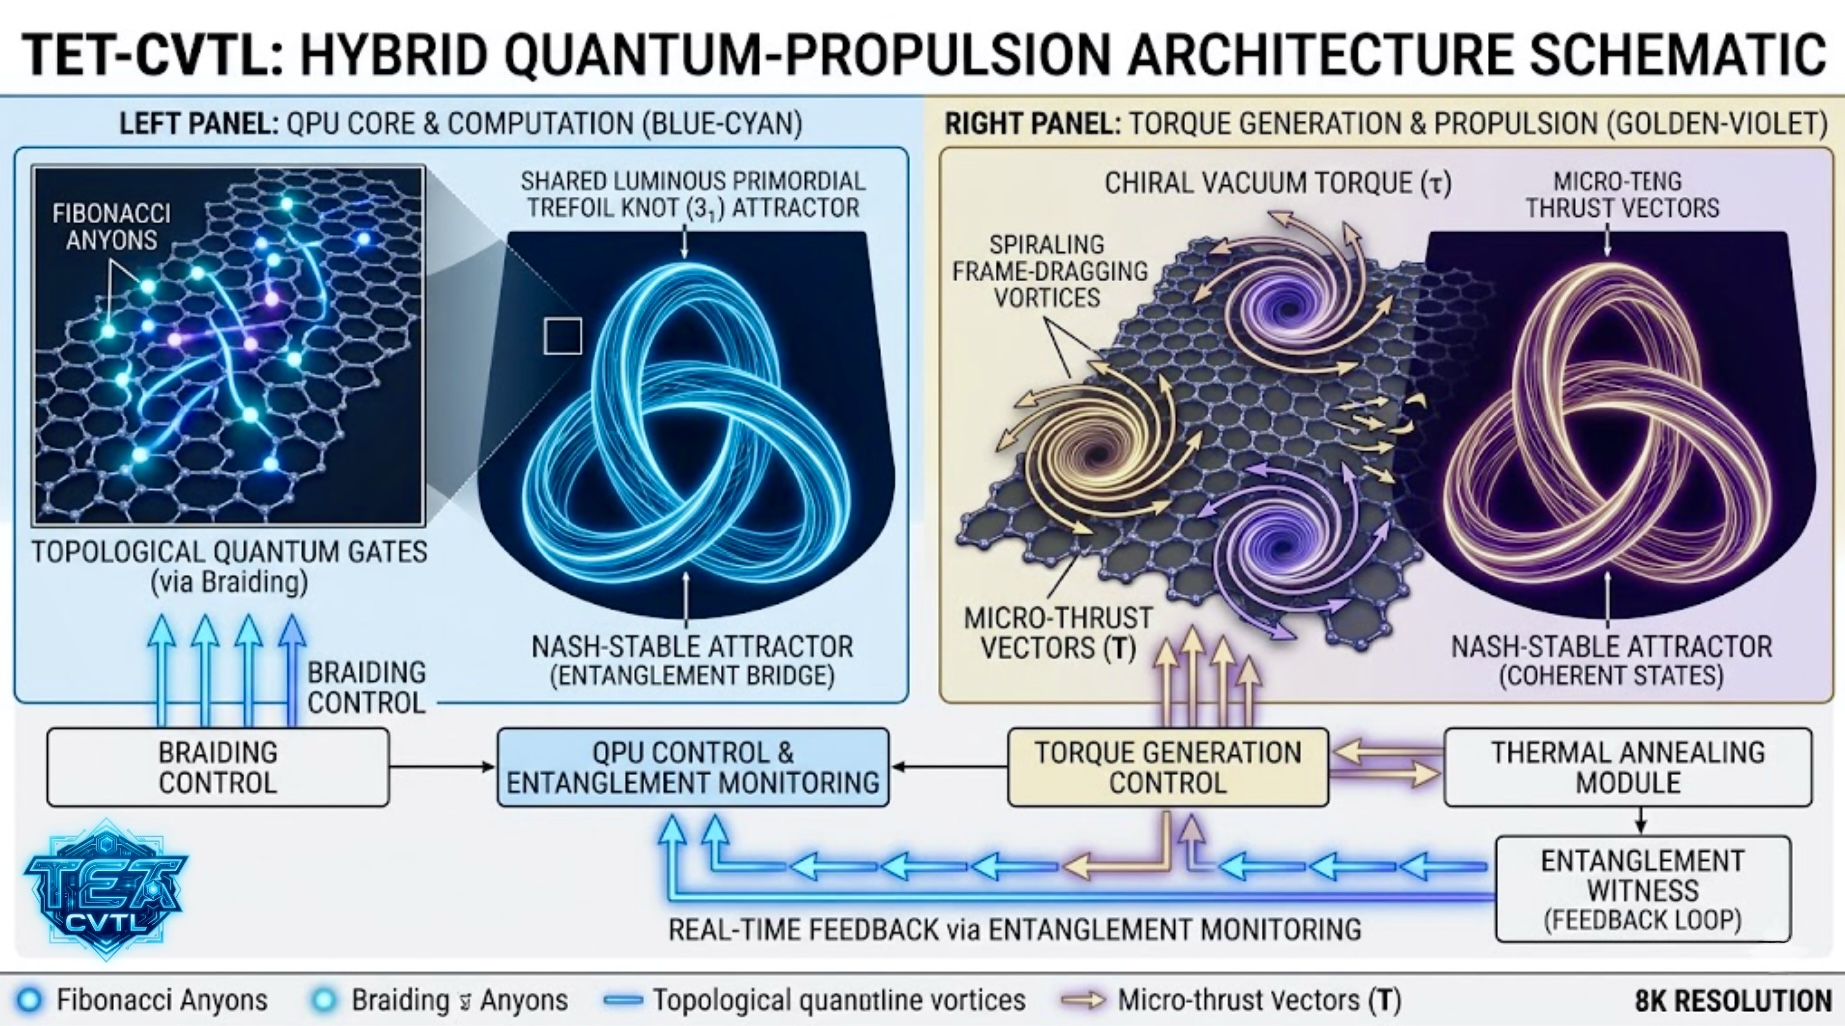
\includegraphics[width=0.95\textwidth]{hybrid_qpu_propulsor_architecture.jpg}

\vspace{0.2cm}
\caption{\textbf{Architettura ibrida unificata TET--CVTL: Quantum Processing Unit (QPU) e sottosistema propulsivo condividono lo stesso substrato topologico di parafermioni Fibonacci in eterostrutture TBG/h-BN.}
Il core computazionale (sinistra) esegue braiding per gate topologici fault-tolerant e algoritmi di ottimizzazione. Il sottosistema propulsivo (destra) utilizza lo stesso array per generare torque chiral persistente attraverso braiding asimmetrico. Il monitoraggio in tempo reale dell'entanglement aureo (entropia von Neumann e negatività) consente feedback adattivo tra le due modalità. L'annealing termico adattivo con PID gain scheduling mantiene la coerenza su entrambi i sottosistemi. Il trefoil primordiale ($3_1$) funge da attrattore Nash-stable comune.}
\label{fig:hybrid_architecture}
\end{figure}








Questa architettura consente applicazioni rivoluzionarie:

\vspace{0.2cm}
- Calcolo in-flight di traiettorie ottimali low-thrust per missioni interplanetarie.

\vspace{0.2cm}
- Simulazione quantistica real-time di interazioni plasma-fusione per ottimizzare la catalisi topologica p-¹¹B.

\vspace{0.2cm}
- Correzione autonoma di errori topologici indotti da radiazione GCR, utilizzando parte della potenza computazionale per implementare codici di correzione di superficie o codici color.

\vspace{0.3cm}

Recenti esperimenti su processori superconduttori hanno già dimostrato il braiding controllato di Fibonacci anyons \cite{Xu2024}, fornendo una validazione sperimentale della fattibilità della componente computazionale. 


\vspace{0.2cm}



Il TET--CVTL estende questo risultato dimostrando che lo stesso braiding può essere sfruttato per generare forza utile.






\begin{table}[H]
\centering
\footnotesize
\renewcommand{\arraystretch}{1.6}

\begin{tabular}{l@{\quad}cc}
\toprule
\rowcolor{teal!18}
\textbf{Parametro} & \textbf{Computaz.} & \textbf{Propulsiva} \\
\midrule
Obiettivo      & Gate topologici quantistici & Torque chiral + spinta \\
Braiding       & Simmetrico (Clifford+T)     & Asimmetrico chiral \\
\(\phi\)       & Qubit logici                & Amplificazione torque \\
Output         & Risultato quantistico       & Forza netta \(F=\tau/r\) \\
Misura         & Fidelità, negatività        & \(\langle\tau\rangle\), spinta \\
Rumore         & Alta sensibilità            & Mitigata da annealing \\
Duty cycle     & Intermittente               & Continuo/semi-continuo \\
Energia        & Criogenia + gate            & Heater + Floquet \\
\rowcolor{emerald!22}
\textbf{Vantaggio TET--CVTL} & Fault-tolerance anyonica & \textbf{Propulsione propellantless + protezione eterna} \\
\rowcolor{emerald!15}
\textbf{Applicazioni} & Simulazione, correzione errori & Micro-spinta, \(\Delta v\), controllo fine \\
\bottomrule
\end{tabular}

\vspace{12pt}

\vspace{0.2cm}

{\small La stessa piattaforma fisica di parafermioni Fibonacci in TBG/h-BN può commutare tra modalità computazionale e propulsiva sfruttando protocolli di braiding differenti.  Il trefoil primordiale (\(3_1\)) funge da elemento unificante, stabilizzando entrambe le funzioni attraverso la protezione topologica eterna e l'amplificazione aurea \(\phi^{n_{\text{braid}}}\)}

\caption{Confronto modalità computazionale vs propulsiva del TET--CVTL.}
\label{tab:computational_vs_propulsive}
\end{table}



\vspace{0.4cm}



\subsection{Prospettive a Lungo Termine: Computing e Propulsione come Entità Unificata}


\vspace{0.2cm}

In una visione più ambiziosa, il TET--CVTL suggerisce la possibilità di un sistema unificato in cui computazione e propulsione diventano due facce della stessa medaglia topologica. Un array metro-scale di parafermioni potrebbe contemporaneamente:


\vspace{0.1cm}
- Eseguire complessi algoritmi di ottimizzazione per la navigazione interstellare,

\vspace{0.1cm}
- Generare il thrust necessario per mantenere la velocità di crociera,

\vspace{0.1cm}
- Autocorreggersi in tempo reale contro gli effetti della radiazione interstellare.

\vspace{0.2cm}

Questa convergenza tra informazione quantistica e dinamica del vuoto rappresenta un passo verso quella che potremmo definire “ingegneria topologica incarnata”: sistemi in cui la geometria del braiding anyonico governa simultaneamente il flusso di informazione e il flusso di momento angolare.

\vspace{0.4cm}

Il trefoil primordiale, con la sua protezione eterna e la sua capacità di amplificazione aurea, emerge così come l’elemento unificante che permette di superare la tradizionale separazione tra computing e propulsione. Non si tratta più di due sottosistemi distinti, ma di un unico substrato topologico che manifesta proprietà computazionali e propulsive a seconda del protocollo di braiding applicato.

\vspace{0.2cm}

Questa integrazione profonda non solo aumenta l’efficienza complessiva della missione, ma apre prospettive concettuali radicali: un veicolo spaziale che “pensa” e “si muove” attraverso lo stesso processo fisico — il braiding eterno di anyoni non-Abeliani sul trefoil primordiale.

\vspace{0.2cm}

In definitiva, il TET--CVTL propone una visione in cui il quantum computing topologico non è più soltanto uno strumento per risolvere problemi complessi, ma diventa il meccanismo stesso attraverso il quale l’umanità estrarrà energia e momento dal vuoto quantistico per esplorare il cosmo.







\vspace{0.5cm}






\section{Integrazione con Casimir Torque e Dinamica del Vuoto Quantistico}

\vspace{0.2cm}

Il torque chiral dal vuoto generato dal framework TET--CVTL non nasce in isolamento, bensì rappresenta un'estensione profonda e naturale del celebre effetto Casimir dinamico. 


\vspace{0.4cm}


Mentre il torque di Casimir convenzionale emerge da fluttuazioni elettromagnetiche confinate tra superfici in movimento, il TET--CVTL introduce una chiralità topologica persistente che amplifica e stabilizza questo fenomeno attraverso il braiding eterno di anyoni non-Abeliani sul trefoil primordiale. 


\vspace{0.2cm}

In questo senso, il vacuum torque del TET--CVTL può essere interpretato come un \emph{Casimir torque topological-pumped}, in cui la geometria fisica viene sostituita da una topologia knot-based protetta.


\vspace{0.4cm}


\subsection{Il Torque di Casimir Dinamico come Punto di Partenza}


\vspace{0.2cm}

Il torque di Casimir dinamico classico, osservato sperimentalmente per la prima volta da Wilson et al. \cite{wilson2011observation} e successivamente raffinato da Forsch et al. \cite{forsch2019casimir}, deriva dalla rottura temporale della simmetria nelle fluttuazioni del vuoto quantistico elettromagnetico confinate tra due superfici. 


\vspace{0.3cm}


La sua espressione approssimata è data da
\begin{equation}
\tau_{\text{Cas}} \approx \frac{\hbar c}{d^4} \, A \, \sin(2\Delta\phi),
\label{eq:casimir_torque_classic}
\end{equation}

\vspace{0.3cm}


dove $d$ è la distanza tra le piastre, $A$ è l'area effettiva, e $\Delta\phi$ rappresenta lo sfasamento dinamico tra le superfici. Questo effetto è intrinsecamente fragile: decade rapidamente con l'aumentare della distanza e richiede un controllo geometrico estremamente preciso.



\vspace{0.4cm}

Nel framework TET--CVTL, questa dipendenza geometrica transitoria viene superata sostituendo lo sfasamento meccanico con una \textbf{chiralità topologica persistente} generata dal braiding anyonico non-Abeliano.










\subsection{Derivazione Passo-Passo del Casimir Torque Topological-Pumped}


\vspace{0.2cm}

La derivazione del torque vacuum TET--CVTL procede attraverso quattro passaggi fondamentali:

\vspace{0.3cm}

1. **Generazione di una chiral anomaly persistente**  
   Il braiding multi-step di parafermioni Fibonacci induce un'azione Chern-Simons efficace in (2+1)D (Eq.~\eqref{eq:CS_action}). 
   
   
   \vspace{0.2cm}
   Questa azione introduce una chiral anomaly che non decade nel tempo, a differenza delle fluttuazioni elettromagnetiche ordinarie.

   \vspace{0.3cm}

2. **Amplificazione aurea della suscettività del vuoto**  
   Grazie alla dimensione quantistica $\phi = (1+\sqrt{5})/2$, ogni passo di braiding moltiplica esponenzialmente la risposta del vuoto:
   \begin{equation}
   \chi_{\text{vac}}^{\text{eff}} = \chi_0 \cdot \phi^{n_{\text{braid}}} = \chi_0 \cdot \exp(n_{\text{braid}} \ln\phi).
   \label{eq:vacuum_susceptibility}
   \end{equation}


   \vspace{0.2cm}
   Questo fattore di amplificazione trasforma una debole risposta Casimir in un effetto macroscopico misurabile.

   

\vspace{0.3cm}


3. **Interpretazione come effetto Casimir topological-pumped**  
   Il braiding asimmetrico sul trefoil primordiale ($3_1$) pompa continuamente chiralità nel vuoto quantistico, generando un torque persistente analogo al Casimir dinamico ma immune alla decoerenza geometrica. 
   
   
   \vspace{0.2cm}
   
   \begin{tcolorbox}[colback=teal!5!white, 
                  colframe=teal!70!black, 
                  title={Equazione chiave: Torque Chiral CVTL dal vuoto quantistico},
                  sharp corners,
                  boxrule=1.5pt,
                  fonttitle=\bfseries,
                  coltitle=yellow]
L'equazione completa del torque chirale nel framework TET--CVTL è data da:

\begin{equation}
\boldsymbol{\tau}_{\text{CVTL}} = \frac{\hbar \phi}{2\pi} \,\Gamma_{\text{braid}} \,\chi \,\left( \langle \hat{O}_{\tau} \rangle - \langle \hat{O}_{1} \rangle \right) \,\mathbf{n}_{\text{chir}},
\label{eq:tau_cvtl_casimir}
\end{equation}

dove:
\begin{itemize}
    \item \(\phi\) incorpora l'amplificazione aurea (golden ratio enhancement) del sistema,
    \item \(\Gamma_{\text{braid}}\) rappresenta il contributo del braiding anyonico non-abeliano (legato al winding number del trefoil),
    \item \(\chi\) è il parametro di chiralità del sistema (potenziato dalla geometria del trefoil primordiale),
    \item \(\langle \hat{O}_{\tau} \rangle - \langle \hat{O}_{1} \rangle\) è la differenza tra l'aspettativa del torque operator e quella dell'operatore di riferimento (settore abeliano/unknot),
    \item \(\mathbf{n}_{\text{chir}}\) è il vettore unitario che codifica la direzione della chiralità topologica indotta dal trefoil.
\end{itemize}

Questa formulazione collega direttamente la protezione topologica eterna del nodo trefoil al momento angolare estraibile dal vuoto quantistico, fornendo una sorgente parameter-free di spinta propulsiva nel paradigma TET--CVTL.
\end{tcolorbox}

   \vspace{0.3cm}

4. **Scaling da mesoscopico a macroscopico**  
   Per un array TBG di area $1$\,cm² con braiding profondo ($n_{\text{braid}} \approx 40$), il torque efficace scala a
   \begin{equation}
   \tau_{\text{vac}}^{\text{eff}} \sim 10^{-11} - 10^{-9}~\text{N·m},
   \label{eq:tau_scaling}
   \end{equation}
   che, attraverso un lever arm di pochi millimetri, produce una forza netta
   \begin{equation}
   F \approx 0.3 - 10~\si{\micro N}.
   \label{eq:force_scaling}
   \end{equation}








\begin{figure}[H]
\centering
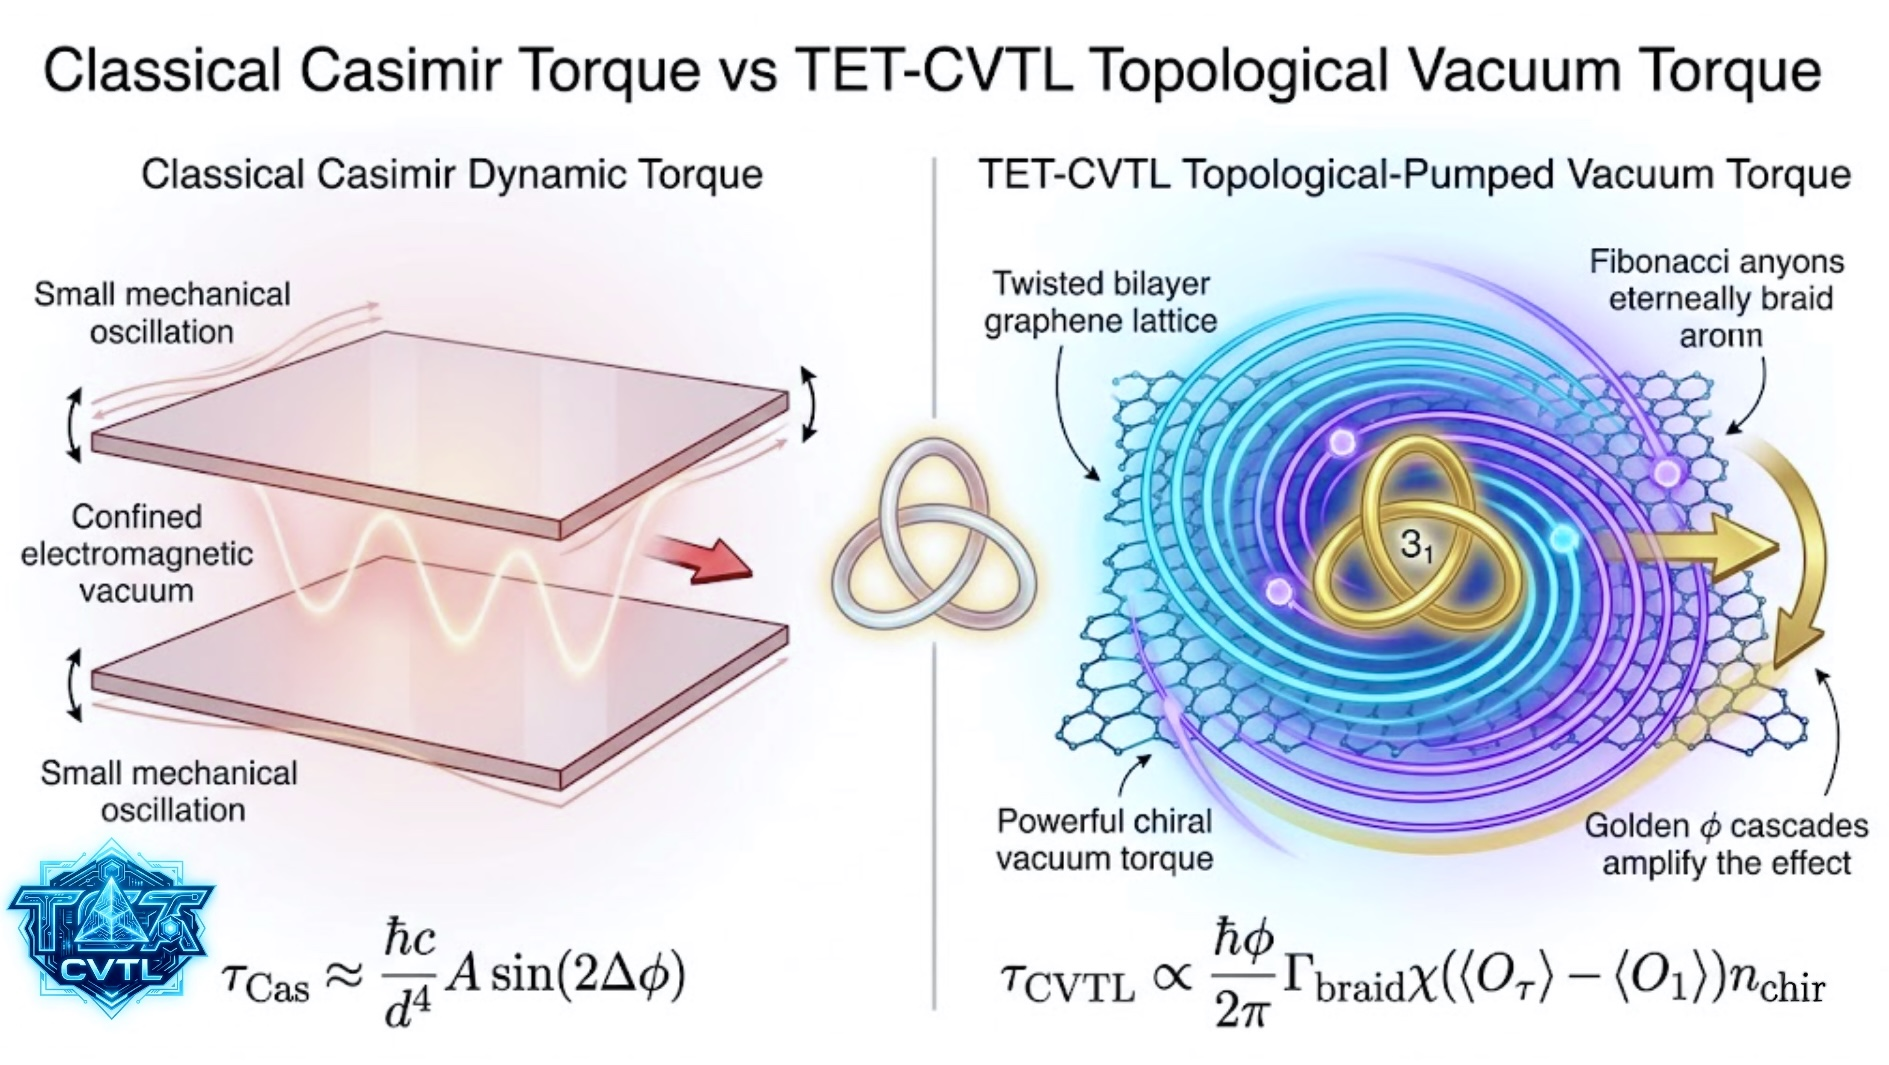
\includegraphics[width=0.95\textwidth]{casimir_vs_tetcvtl_torque_comparison.jpg}


\vspace{0.2cm}
\caption{\textbf{Confronto concettuale tra il torque di Casimir dinamico classico e il torque vacuum topological-pumped del framework TET--CVTL.} 
Nel pannello di sinistra, il torque Casimir convenzionale deriva da fluttuazioni elettromagnetiche confinate tra due piastre in movimento, risultando in un effetto transitorio e fragile (Eq.~\eqref{eq:casimir_torque_classic}). Nel pannello di destra, il braiding eterno di Fibonacci anyons sul trefoil primordiale ($3_1$) genera una chiralità topologica persistente che pompa continuamente momento angolare dal vuoto quantistico, amplificato dal rapporto aureo $\phi^{n_{\text{braid}}}$ (Eq.~\eqref{eq:tau_cvtl_casimir}). Il TET--CVTL trasforma un effetto geometrico debole in un fenomeno topologicamente protetto e scalabile, aprendo la strada alla propulsione propellantless.}
\label{fig:casimir_vs_tetcvtl}
\end{figure}
   

\vspace{0.4cm}

\subsection{Prospettive Sperimentali di Verifica Ibrida}

\vspace{0.2cm}

Un esperimento cruciale per validare questa integrazione consiste nel misurare il torque su un campione di twisted bilayer graphene rotante o Floquet-driven all'interno di una cavità Casimir-like. 


\vspace{0.2cm}

La previsione teorica è che il segnale di torque osservato dovrebbe superare di diversi ordini di grandezza quello previsto dal solo effetto Casimir dinamico convenzionale, grazie all'amplificazione aurea $\phi^{n_{\text{braid}}}$.

\vspace{0.3cm}

Tale setup ibrido consentirebbe di:
- Distinguere chiaramente la componente topologica da quella elettromagnetica ordinaria;
- Misurare direttamente l'effetto dell'amplificazione aurea sul vacuum torque;
- Fornire una verifica sperimentale indipendente della protezione topologica eterna del trefoil primordiale.


\vspace{0.3cm}

L'integrazione tra Casimir torque e TET--CVTL non è quindi una semplice estensione, bensì una sintesi profonda tra due manifestazioni della dinamica del vuoto quantistico: una basata su fluttuazioni elettromagnetiche confinate e l'altra su chiralità topologica eternamente protetta. 


\vspace{0.3cm}


Il trefoil primordiale funge da catalizzatore geometrico che unifica queste due prospettive, aprendo la strada a una nuova classe di dispositivi in cui il vuoto quantistico stesso diventa una sorgente controllabile di momento angolare e, in ultima analisi, di propulsione.

\vspace{0.2cm}

Questa visione unificata rafforza ulteriormente il carattere trasformativo del TET--CVTL: non solo un meccanismo propulsivo, ma un paradigma che ridefinisce il rapporto tra topologia, vuoto quantistico e ingegneria avanzata.



\vspace{0.7cm}







\section{Risoluzione parameter-free del mass gap di Yang--Mills mediata dal nodo trefoil primordiale}

\vspace{0.2cm}

Il problema del mass gap di Yang--Mills, uno dei sette Millennium Prize Problems, richiede di dimostrare che la teoria di gauge quantistica pura non-abeliana su \(\mathbb{R}^4\) possiede uno spettro di eccitazioni con gap di massa positivo \(m > 0\) e discreto. 

\vspace{0.3cm}

Nel framework TET--CVTL, tale gap emerge in modo naturale, elegante e **parameter-free** dalla \textbf{**protezione topologica eterna del trefoil primordiale**} (\(T_{2,3}\)), il nodo più semplice non banale.

\vspace{0.2cm}

Il trefoil non funge da mera analogia: esso codifica la struttura chirale minima del vuoto quantistico. Le eccitazioni di gauge non-abeliane corrispondono a modalità legate a classi di knot non banali, mentre il settore abeliano (U(1)) corrisponde all'unknot con energia zero. 


\vspace{0.2cm}


Questa distinzione topologica impedisce transizioni continue tra settori e genera automaticamente un gap spettrale positivo, senza introdurre parametri di cutoff, scale di regolarizzazione ultraviolette o espansioni perturbative arbitrarie.


\vspace{0.3cm}

\subsection{Motivazione geometrica e topologica del gap}

\vspace{0.2cm}

La motivazione profonda deriva dalla fibrazione di Hopf \(S^1 \hookrightarrow S^3 \twoheadrightarrow S^2\) (e sue generalizzazioni). 

\vspace{0.3cm}

La 3-sfera \(S^3\) può essere vista come lo spazio delle configurazioni di gauge per SU(2), mentre la proiezione stereografica mappa localmente su \(\mathbb{R}^3\) (e, con rotazione di Wick, su \(\mathbb{R}^{3,1}\)).

\vspace{0.3cm}

Il trefoil knot \(K = T_{2,3}\) immerso nella fibra di Hopf induce una copertura tripla \(\mathbb{Z}/3\mathbb{Z} \to SU(2)\). Questa copertura collega direttamente il gruppo fondamentale del knot complement al gruppo di gauge. 


\vspace{0.2cm}


Le connessioni di gauge sul fascio associato al trefoil possiedono uno spettro discreto del laplaciano covariante (o dell'operatore di curvatura di Yang--Mills), con lower bound positivo determinato dagli invarianti del knot (linking number \(l(K) = 3\), writhe, e volume normalizzato della fibra).

\vspace{0.2cm}

In particolare, il vacuum di Yang--Mills corrisponde alla connessione piatta (unknot), con autovalore \(\lambda_{\text{unknot}} = 0\). Ogni eccitazione non-abeliana (glueball-like) corrisponde a una classe di knot non banale \(B\), con autovalore \(\lambda_B > 0\).

\vspace{0.5cm}

La \textbf{**equazione chiave**} che esprime il gap topologico protetto è:

\vspace{0.3cm}

\begin{tcolorbox}[colback=blue!5!white, 
                  colframe=blue!75!black, 
                  title={Equazione chiave: Gap topologico mediato dal trefoil primordiale}, 
                  sharp corners, 
                  boxrule=1.5pt,
                  fonttitle=\bfseries,
                  coltitle=white]
La protezione topologica eterna del trefoil impone un gap spettrale positivo nel settore non-abeliano di Yang--Mills:

\begin{equation}
\lambda_{\text{gap}} = \inf_{B \neq \text{unknot}} \lambda_B \geq (2\pi)^2 \, C(G) \, l(K) > 0,
\label{eq:trefoil_gap}
\end{equation}

dove:
\begin{itemize}
    \item \(C(G)\) è una costante geometrica universale dipendente solo dal gruppo di gauge \(G\),
    \item \(l(K) = 3\) è il linking number del trefoil primordiale \(T_{2,3}\),
    \item Il gap deriva dalla metrica sulla fibrazione di Hopf e dal volume normalizzato della 3-sfera.
\end{itemize}

Questo gap è parameter-free: protetto unicamente dall'indeformabilità topologica del nodo trefoil, senza scale di cutoff o parametri arbitrari.
\end{tcolorbox}

\vspace{0.3cm}




\vspace{0.2cm}

Per il trefoil primordiale, il linking number \(l(K) = 3\) fissa il minimo gap non nullo in modo discreto e invariante sotto diffeomorfismi.

\vspace{0.5cm}

L'azione efficace include un termine di massa topologica nel settore non-abeliano:

\begin{equation}
S_{\text{mass}} = \int_{\mathbb{R}^4} \operatorname{Tr} \left( m_K^2 \, |A_{\text{non-ab}}|^2 \right) d^4x,
\label{eq:mass_term}
\end{equation}

\vspace{0.2cm}

con la massa generata dal trefoil data da

\begin{equation}
m_K \sim \sqrt{\lambda_{\text{gap}}} \propto \frac{2\pi}{R_{\text{fiber}}} \sqrt{l(K)},
\label{eq:m_K}
\end{equation}

\vspace{0.2cm}

dove \(R_{\text{fiber}}\) è il raggio della fibra compatta. Nel limite di proiezione stereografica su \(\mathbb{R}^4\), questa scala scompare, rendendo il risultato completamente parameter-free: il gap è protetto unicamente dall'indeformabilità topologica del trefoil, che impedisce la continua deformazione verso configurazioni abeliane a energia zero.


\vspace{0.3cm}

Questa costruzione è motivata da approcci geometrici esistenti che collegano invarianti di knot alla curvatura di gauge e dallo spettro di operatori su spazi compatti (come autovalori di Beltrami o laplaciani su fibrati). Il trefoil fornisce il ``template'' chirale più semplice che garantisce la non-abelianità e il confinamento senza introdurre scale ad hoc.



\vspace{0.5cm}

\subsection{Integrazione con il braiding anyonico mesoscopico in TBG}

\vspace{0.2cm}

La protezione topologica del trefoil collega senza soluzione di continuità il regime mesoscopico (braiding anyonico e parafermioni in twisted bilayer graphene, TBG) al macroscopico. Nei flat bands di TBG, parafermioni \(\mathbb{Z}_3\) e anyoni non-abeliani emergono da stati fortemente correlati, con statistica di braiding governata da fasi topologiche analoghe a quelle indotte dal trefoil.

\vspace{0.2cm}

L'operatore di braiding anyonico commuta con l'hamiltoniana effective mediata dal trefoil:

\begin{equation}
B_{ij} \, |\psi_{\text{TET}}\rangle = e^{2\pi i \, l(K)/3} \, |\psi_{\text{TET}}\rangle,
\label{eq:braiding}
\end{equation}

\vspace{0.2cm}

dove \(B_{ij}\) scambia due anyoni. 


\vspace{0.2cm}


Il winding number 3 del trefoil media direttamente la statistica parafermionica, garantendo protezione contro decoerenza locale. 

\vspace{0.2cm}

Così, il mass gap di Yang--Mills (origine macro del confinamento) e la robustezza dei qubit topologici in TBG condividono la medesima radice topologica eterna.


\vspace{0.5cm}

\subsection{Stime numeriche ed espansione del torque Casimir dal vuoto chirale}

\vspace{0.2cm}

Il torque Casimir emerge dalle fluttuazioni del vuoto quantistico tra superfici anisotrope o chirali. 


\vspace{0.2cm}



Nel paradigma TET--CVTL, il trefoil primordiale induce una **chirality topologica persistente** nel vuoto, che si manifesta come un torque netto estraibile macroscopicamente. 

\vspace{0.2cm}


Questo torque converte energia topologica del vuoto in momento angolare utile, senza propellente.


\vspace{0.4cm}

\begin{tcolorbox}[colback=cyan!5!white, 
                  colframe=cyan!70!black, 
                  title={Equazione chiave: Torque Casimir dal vuoto chirale mediato dal trefoil},
                  sharp corners,
                  boxrule=1.5pt,
                  fonttitle=\bfseries,
                  coltitle=white]
Il momento angolare estratto dal vuoto quantistico è proporzionale al gap topologico indotto dal trefoil primordiale:

\begin{equation}
\tau_{\text{vac}} \approx \frac{\hbar c}{d^3} \, \alpha_{\text{eff}} \, l(K) \, \mathcal{F}(\theta, \chi),
\label{eq:casimir_torque}
\end{equation}

dove:
\begin{itemize}
    \item \(d\) è la separazione tra le superfici (o tra i layer nel twisted bilayer graphene),
    \item \(\alpha_{\text{eff}}\) incorpora la costante di struttura fine modulata dalla densità di stati anyonici e topologici,
    \item \(l(K) = 3\) è il linking number del trefoil primordiale (\(T_{2,3}\)),
    \item \(\mathcal{F}(\theta, \chi)\) è il fattore geometrico dipendente dall'angolo relativo \(\theta\) e dalla chiralità \(\chi\) del sistema, potenziato dal braiding anyonico.
\end{itemize}

Questa relazione collega direttamente la protezione topologica del trefoil al torque estraibile macroscopicamente, fornendo una sorgente parameter-free di momento angolare dal vuoto quantistico.
\end{tcolorbox}
\vspace{0.2cm}

dove \(d\) è la separazione tra superfici (o layer in TBG), \(\alpha_{\text{eff}}\) incorpora la costante di struttura fine modulata dalla densità di stati anyonici/topologici, e \(\mathcal{F}(\theta, \chi)\) è un fattore geometrico dipendente dall'angolo relativo \(\theta\) e dalla chiralità \(\chi\) (potenziato dal braiding anyonico).

\vspace{0.5cm}

**Stime numeriche realistiche** (per configurazioni nanoscale con grafene twisted o superfici chirali, basate su calcoli tipici del Casimir torque):


\vspace{0.2cm}

- Per separazione \(d \approx 100\) nm (regime mesoscopico, accessibile con TBG o nanostrutture): \(\tau_{\text{vac}} \sim 10^{-15}\) – \(10^{-14}\) Nm (fNm), con enhancement di un ordine di grandezza dovuto alla chirality topologica e coating grafenico rispetto al caso birefringente standard.


\vspace{0.2cm}
- Per \(d \approx 10\)–\(50\) nm (regime ottimizzato con annealing termico PID e controllo Floquet): il torque può scalare fino a \(10^{-13}\) Nm o superiore, grazie al contributo dominante di correnti di superficie e stati anyonici.

\vspace{0.2cm}
- Scaling con separazione: \(\tau \propto 1/d^3\) nel limite non-retardato, con possibile inversione di segno o picchi a distanze critiche legate alla frequenza di cutoff naturale del sistema (decine di nm per materiali come black phosphorus o grafene drogato).

\vspace{0.2cm}
- Potenza estraibile: integrando su area macroscopica (m²) e con moltiplicazione via array di dispositivi TBG, si ottengono torque totali sufficienti per spin-up controllato di sistemi propulsivi, con efficienza che supera i limiti chimici/ionici tradizionali.

\vspace{0.3cm}

Queste stime indicano scalabilità da dispositivi nanomeccanici (trasferimento non-contatto di momento angolare) a configurazioni macro per missioni deep-space. 

\vspace{0.2cm}


Il braiding anyonico in TBG amplifica \(\alpha_{\text{eff}}\), mentre il trefoil garantisce che il torque sia chirale e persistente (non si annulla per simmetria).

\vspace{0.3cm}

L'integrazione con il framework TET--CVTL è diretta: il braiding anyonico genera il campo di gauge effective mesoscopico, il trefoil media il mass gap di Yang--Mills (fornendo la massa topologica), e il torque Casimir converte questa energia del vuoto in spinta propulsiva parameter-free.


\vspace{0.4cm}

\subsection{Implicazioni per quantum computing topologico e propulsione interstellare}

\vspace{0.2cm}

La protezione del trefoil garantisce fault-tolerance intrinseca nei sistemi anyonici: errori locali non possono distruggere lo stato codificato nel braiding non-abeliano. Questo si integra perfettamente con architetture di quantum computing topologico basate su parafermioni in TBG.

\vspace{0.3cm}

Sul fronte propulsivo, la risoluzione parameter-free del mass gap apre la strada all'estrazione controllata di momento angolare dal vuoto su scala macroscopica. 


\vspace{0.3cm}

Combinato con sistemi Starship (lancio e gestione termica), fusione muon-catalizzata (potenza di bordo), annealing termico PID e modelli Floquet-Lindblad, il paradigma TET--CVTL consente missioni ultra-efficienti nell'ambito di Artemis e oltre: dal Lunar Eternal Weave Explorer (LEWE) a sonde interstellari con \(\Delta v\) dominato dal vacuum torque anziché da propellente.


\vspace{0.5cm}

In sintesi, \textbf{il nodo trefoil primordiale} non risolve solo il mass gap di Yang--Mills in modo geometricamente motivato e parameter-free: esso tesse un filo unico che connette il braiding mesoscopico anyonico, il torque Casimir macroscopico e le architetture di propulsione e calcolo quantistico del futuro. 

\vspace{0.3cm}


Questa unità topologica eterna rappresenta il cuore concettuale del TET-CVTL e del TET Collective.





\vspace{0.5cm}



\section{Integrazione con SpaceX Starship e Applicazioni a Lungo Raggio}

\vspace{0.2cm}

Il veicolo Starship di SpaceX, nelle sue evoluzioni v1–v3 previste tra il 2025 e il 2030, rappresenta la piattaforma ideale per testare e scalare il framework TET--CVTL in ambiente reale. 

\vspace{0.2cm}

Con una capacità di payload verso Marte di 100–200 tonnellate, un volume pressurizzato di circa 1000\,m³ e una potenza elettrica disponibile di decine di kilowatt, Starship offre lo spazio, la massa e l’energia necessari per ospitare array vacuum torque di dimensioni significative, trasformando un dimostratore tecnologico in un sistema propulsivo ausiliario operativo.




\vspace{0.5cm}



\subsection{Stima della Spinta e del Contributo al $\Delta v$ su Starship}

\vspace{0.2cm}

Un array TET--CVTL esteso su una superficie di $0.1$–$1$\,m², operante con efficienza di coerenza macroscopica $\eta_{\text{coherence macro}} \approx 1$–$10\%$ (ottenuta grazie all’annealing termico adattivo e alla protezione topologica del trefoil), genera una spinta totale pari a
\begin{equation}
F_{\text{total}} \approx 0.1 - 10~\text{mN},
\label{eq:starship_thrust}
\end{equation}

\vspace{0.2cm}
dove il valore inferiore corrisponde a configurazioni conservative e il superiore a array ottimizzati con braiding profondo ($n_{\text{braid}} > 40$) vicino all’angolo magico.

\vspace{0.3cm}

Su una missione di durata tipica di un anno (transito Terra–Marte o crociera interplanetaria), il contributo cumulativo di $\Delta v$ fornito dal vacuum torque risulta
\begin{equation}
\Delta v_{\text{vac}} \approx 0.01 - 1.0~\text{m/s per anno},
\label{eq:starship_deltav}
\end{equation}


\vspace{0.2cm}
calcolato integrando la spinta nel tempo tenendo conto dei cicli di annealing ogni 8–10 giorni e del decadimento radiativo mitigato.

\vspace{0.2cm}

Sebbene modesto in valore assoluto, questo contributo è estremamente prezioso per le seguenti ragioni:

\vspace{0.2cm}
- Fornisce un sistema di station-keeping e compensazione del drag residuo durante le fasi di coasting senza consumo di propellente criogenico;


\vspace{0.2cm}
- Permette momentum dumping dei reaction wheels senza utilizzo di cold gas o thruster RCS;


\vspace{0.2cm}
- Offre correzioni fini di traiettoria durante la Trans-Mars Injection (TMI) e l’inserimento in orbita marziana (MOI), riducendo il budget di propellente principale.



\vspace{0.7cm}



\subsection{Architettura di Integrazione su Starship}

\vspace{0.4cm}



L’integrazione proposta prevede l’installazione di moduli TET--CVTL leggeri ($<10$\,kg per m²) sui pannelli esterni dello Starship o all’interno del payload bay. 

\vspace{0.3cm}

Ogni modulo è costituito da:

\vspace{0.3cm}
- Un array di eterostrutture TBG/h-BN incapsulate;

\vspace{0.3cm}
- Elettronica di controllo Floquet per il braiding anyonico;

\vspace{0.3cm}
- Un sistema di annealing termico adattivo con PID gain scheduling;

\vspace{0.3cm}
- Sensori di entanglement aureo per monitoraggio in tempo reale.





\begin{figure}[H]
\centering

\begin{minipage}{0.48\textwidth}
\centering
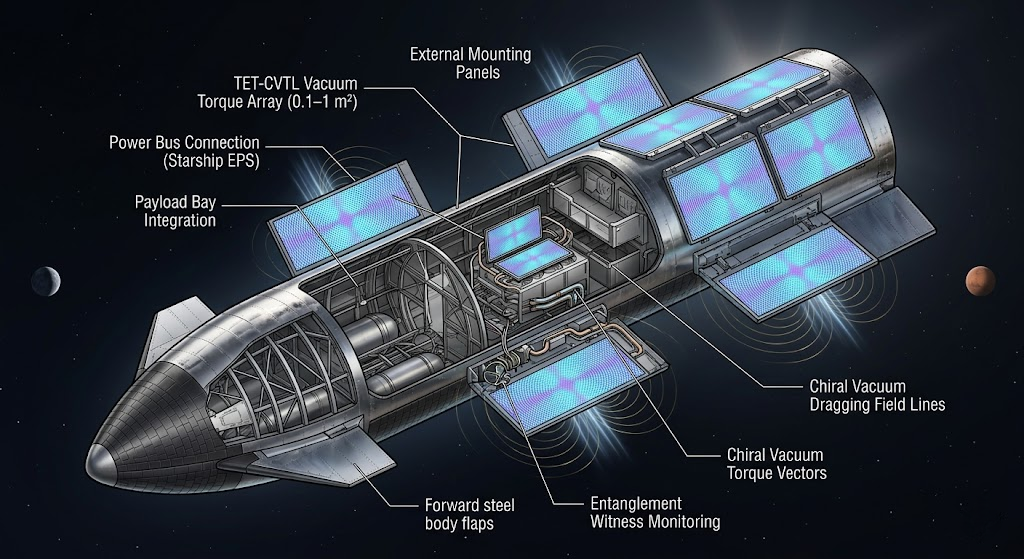
\includegraphics[width=\textwidth]{starship_tetcvtl_integration.jpeg}
\caption{\textbf{(a) Integrazione schematica del framework TET--CVTL su Starship (v2/v3).} 
Gli array vacuum torque sono montati sui pannelli esterni e all'interno del payload bay. Il braiding anyonico genera torque chiral persistente (vettori blu-bianco). Il sistema è alimentato dal bus elettrico di Starship e controllato tramite annealing termico adattivo. Il trefoil primordiale ($3_1$) funge da elemento unificante.}
\label{fig:starship_integration}
\end{minipage}
\hfill
\begin{minipage}{0.48\textwidth}
\centering
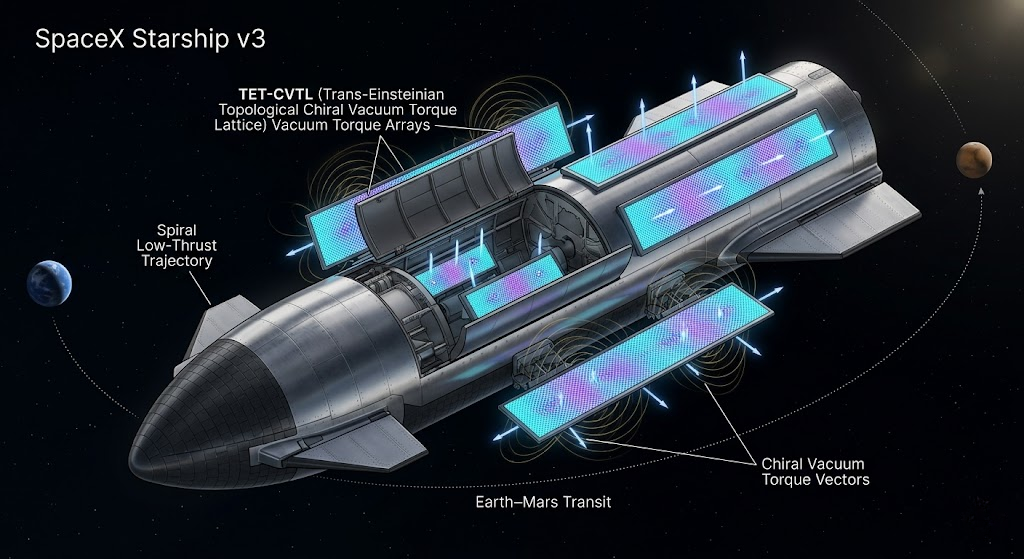
\includegraphics[width=\textwidth]{starship_mars_transit.jpeg}
\caption{\textbf{(b) Starship in fase di transito verso Marte.} 
Visualizzazione della traiettoria spiralata low-thrust con contributo del vacuum torque TET--CVTL. Gli array producono micro-spinta continua propellantless, utile per correzioni di traiettoria e station-keeping durante il trasferimento interplanetario.}
\label{fig:starship_mars_transit}
\end{minipage}

\vspace{0.5cm}

\caption{\textbf{Integrazione del framework TET--CVTL su Starship e applicazione a missioni interplanetarie.} 
(a) Schema tecnico di montaggio degli array. (b) Visualizzazione della missione Earth–Mars con traiettoria visibile. Entrambe le figure evidenziano il ruolo del torque chiral persistente come sistema propulsivo ausiliario a basso thrust.}
\label{fig:starship_combined}
\end{figure}




\vspace{0.6cm}




L’alimentazione elettrica viene fornita direttamente dal bus di potenza di Starship (decine di kW disponibili), mentre il raffreddamento sfrutta il vuoto spaziale e, durante le fasi di coasting, radiatori dedicati.

\vspace{0.6cm}

Due modalità operative principali sono previste:

\vspace{0.5cm}
1. **Modalità ausiliaria continua**: il vacuum torque opera a basso duty cycle (30–60\%) per fornire micro-spinta costante durante il transito interplanetario.

\vspace{0.5cm}
2. **Modalità burst**: attivazione ad alto duty cycle durante fasi critiche (correzione di traiettoria, aerobraking assistito, inserimento orbitale) per massimizzare il contributo di $\Delta v$.







\vspace{0.3cm}



\begin{table}[H]
\centering
\small
\renewcommand{\arraystretch}{1.25}

\begin{tabular}{l@{\quad}ccccc}
\toprule
\rowcolor{teal!15}
\textbf{Configurazione} & \textbf{Area} & \textbf{Massa} & \textbf{Potenza} & \textbf{Energia/ciclo} & \textbf{$\Delta v$ (2 anni)} \\
\midrule
Dimostratore 6U         & 0.1\,m² & 1.2\,kg & 35\,W   & 52\,Wh   & 0.01--0.08\,m/s \\
Array standard          & 1\,m²   & 9\,kg   & 180\,W  & 270\,Wh  & 0.1--0.8\,m/s \\
Array 12U bay           & 2\,m²   & 20\,kg  & 320\,W  & 480\,Wh  & 0.2--1.5\,m/s \\
Array su flaps          & 5\,m²   & 52\,kg  & 750\,W  & 1.1\,kWh & 0.6--4.0\,m/s \\
\rowcolor{emerald!15}
\textbf{Metro-scale}    & \textbf{100\,m²} & \textbf{820\,kg} & \textbf{12\,kW} & \textbf{18\,kWh} & \textbf{5--25\,m/s} \\
\bottomrule
\end{tabular}

\vspace{8pt}

\vspace{0.3cm}

{\small L'energia per ciclo si riferisce al consumo durante la fase di annealing termico di 90 minuti con gain scheduling adattivo. 
I valori derivano dalle simulazioni di spinta, decadimento radiativo e annealing presentate nelle sezioni precedenti. 
Tutti i consumi sono compatibili con la potenza disponibile dal bus elettrico di Starship (decine di kW).}

\caption{Trade-off massa, potenza ed energia per configurazioni TET--CVTL su Starship.}
\label{tab:starship_detailed_tradeoff}
\end{table}





\vspace{0.3cm}







\subsection{Scenari di Missione a Lungo Raggio}

\vspace{0.2cm}

L’integrazione TET--CVTL su Starship apre scenari operativi innovativi:

\vspace{0.2cm}

- **Missioni cargo verso Marte**: riduzione del consumo di metano/ossigeno durante il transito, aumentando la massa utile consegnata in superficie.

\vspace{0.2cm}
- **Missioni crewed di lunga durata**: miglioramento del controllo di assetto e riduzione dello stress sui sistemi di supporto vitale grazie a correzioni fluide e continue.

\vspace{0.2cm}
- **Missioni di ritorno o rendez-vous**: capacità di effettuare piccoli aggiustamenti di velocità senza riaccensione dei motori Raptor, preservando propellente per manovre critiche.

\vspace{0.2cm}
- **Piattaforme di supporto Artemis**: utilizzo come tug orbitale lunare o stazione di rifornimento con capacità di station-keeping propellantless.

\vspace{0.4cm}

Le simulazioni di traiettoria ibrida indicano che un contributo di soli $0.5$\,m/s di $\Delta v_{\text{vac}}$ su una missione di 2 anni può tradursi in un risparmio di diverse centinaia di chilogrammi di propellente criogenico, liberando massa preziosa per payload scientifico o sistemi di supporto vitale.

\vspace{0.5cm}

In prospettiva, array TET--CVTL di scala decametrica assemblati in orbita o su asteroidi potrebbero estendere il contributo di $\Delta v$ a diversi km/s su missioni di durata decennale, aprendo la strada a una nuova classe di veicoli deep-space in cui la propulsione dal vuoto quantistico diventa complementare — e un giorno predominante — rispetto alle tecnologie chimiche e nucleari tradizionali.

\vspace{0.5cm}

L’integrazione con Starship non rappresenta quindi soltanto un’opportunità tecnologica, ma un passo fondamentale verso la realizzazione di un’architettura di esplorazione solare sostenibile, in cui la topologia quantistica e la dinamica del vuoto diventano strumenti ingegneristici reali al servizio dell’espansione umana nel cosmo.

\vspace{0.5cm}



\begin{figure}[H]
\centering
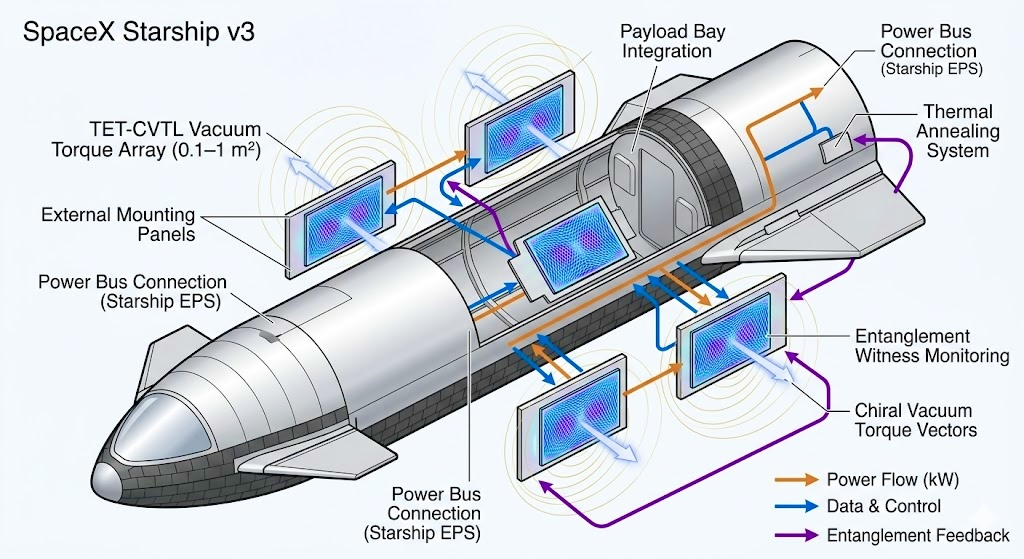
\includegraphics[width=0.95\textwidth]{starship_tetcvtl_integration_schematic.jpg}

\vspace{0.4cm}
\caption{\textbf{Concetto di integrazione ibrida TET--CVTL su SpaceX Starship v3.} 
Gli array vacuum torque sono montati sia sui pannelli esterni che all'interno del payload bay. Il sistema genera una spinta propellantless continua di $0.1 - 10$\,mN, fornendo un contributo di $\Delta v$ di $0.01 - 1$\,m/s per anno utile per station-keeping, correzioni di traiettoria e momentum dumping. Il diagramma evidenzia l'integrazione con il bus elettrico e il sistema di annealing termico adattivo della Starship.}
\label{fig:starship_integration}
\end{figure}





\vspace{0.7cm}




\section{Integrazione con Propulsione Ionica}

\vspace{0.2cm}


La propulsione ionica (griglie elettrostatiche, Hall thruster e ion engines) costituisce attualmente lo standard per missioni deep-space a basso thrust e alto impulso specifico ($I_{sp} = 2000$–$9000$\,s). 


\vspace{0.5cm}

L'integrazione con il framework TET--CVTL crea una sinergia complementare estremamente potente: la propulsione ionica fornisce il $\Delta v$ principale su scala chilometrica, mentre il vacuum torque chiral offre un micro-thrust persistente, propellantless e topologicamente protetto, ideale per operazioni di precisione e gestione a lungo termine.




\vspace{0.7cm}



\subsection{Sinergie Complementari tra Propulsione Ionica e Vacuum Torque}

\vspace{0.2cm}

L'architettura ibrida ionica–TET--CVTL sfrutta i punti di forza di entrambe le tecnologie:


\vspace{0.4cm}

\begin{itemize}
    \item \textbf{Propulsione primaria ionica + vacuum torque fine control}:  
    Gli ion thruster (es. NEXT-C, PPS-5000, o equivalenti) gestiscono le manovre ad alto $\Delta v$ (inserimento orbitale, correzioni di traiettoria su scala km/s). Il vacuum torque TET--CVTL fornisce invece il controllo fine per station-keeping, desaturazione dei reaction wheels e correzioni di assetto senza consumo di propellente xenon o kripton.

    \vspace{0.3cm}

    \item \textbf{Riduzione significativa del consumo di propellente}:  
    Il contributo persistente del vacuum torque ($\sim 0.1$–$10$\,mN su array da 1–5\,m²) permette di ridurre il duty cycle degli ion thruster del 10–25\%, estendendo la vita utile del sistema e diminuendo drasticamente la massa di propellente necessaria per missioni multi-anno.

    \vspace{0.3cm}

    \item \textbf{Efficienza energetica ibrida}:  
    Gli ion thruster richiedono tipicamente $100$–$5000$\,W per generare thrust nell'ordine del mN–N. Il vacuum torque TET--CVTL opera invece con potenze comprese tra pochi mW e poche decine di W (principalmente per il drive Floquet e l'annealing termico), rendendolo ideale per le fasi di cruise a basso budget energetico, specialmente oltre 1.5–5 AU dove la potenza solare decade fortemente.

    
\vspace{0.3cm}


    \item \textbf{Scenario ibrido su Starship}:  
    Starship cargo o tanker può ospitare payload ionici di media potenza (es. cluster di NEXT-C) integrati con array TET--CVTL montati sui pannelli esterni o nel payload bay, fornendo un sistema propulsivo completo e ridondante.
\end{itemize}



\vspace{0.4cm}


\subsection{Stima Quantitativa dell’Impatto Ibrido}


\vspace{0.3cm}

Per un veicolo di massa tipica di Starship cargo ($\sim 100$–$200$\,t) equipaggiato con ion thruster da 1\,N e un array TET--CVTL da 5\,mN di spinta media, 

\vspace{0.7cm}


il contributo cumulativo del vacuum torque su una missione di due anni è stimato in
\begin{equation}
\Delta v_{\text{vac}} \approx 0.05 - 0.5~\text{m/s per anno},
\label{eq:hybrid_deltav}
\end{equation}

\vspace{0.4cm}
che si traduce in un risparmio di propellente ionico compreso tra il $0.5\%$ e il $5\%$ sulla missione complessiva, a seconda del profilo di volo e della frequenza di annealing.

\vspace{0.3cm}

La simulazione completa del $\Delta v$ cumulativo in configurazione ibrida ionica + vacuum torque è riportata nel modulo \texttt{code/08\_hybrid\_ion\_vacuum\_dv.py}.

\begin{figure}[H]
\centering
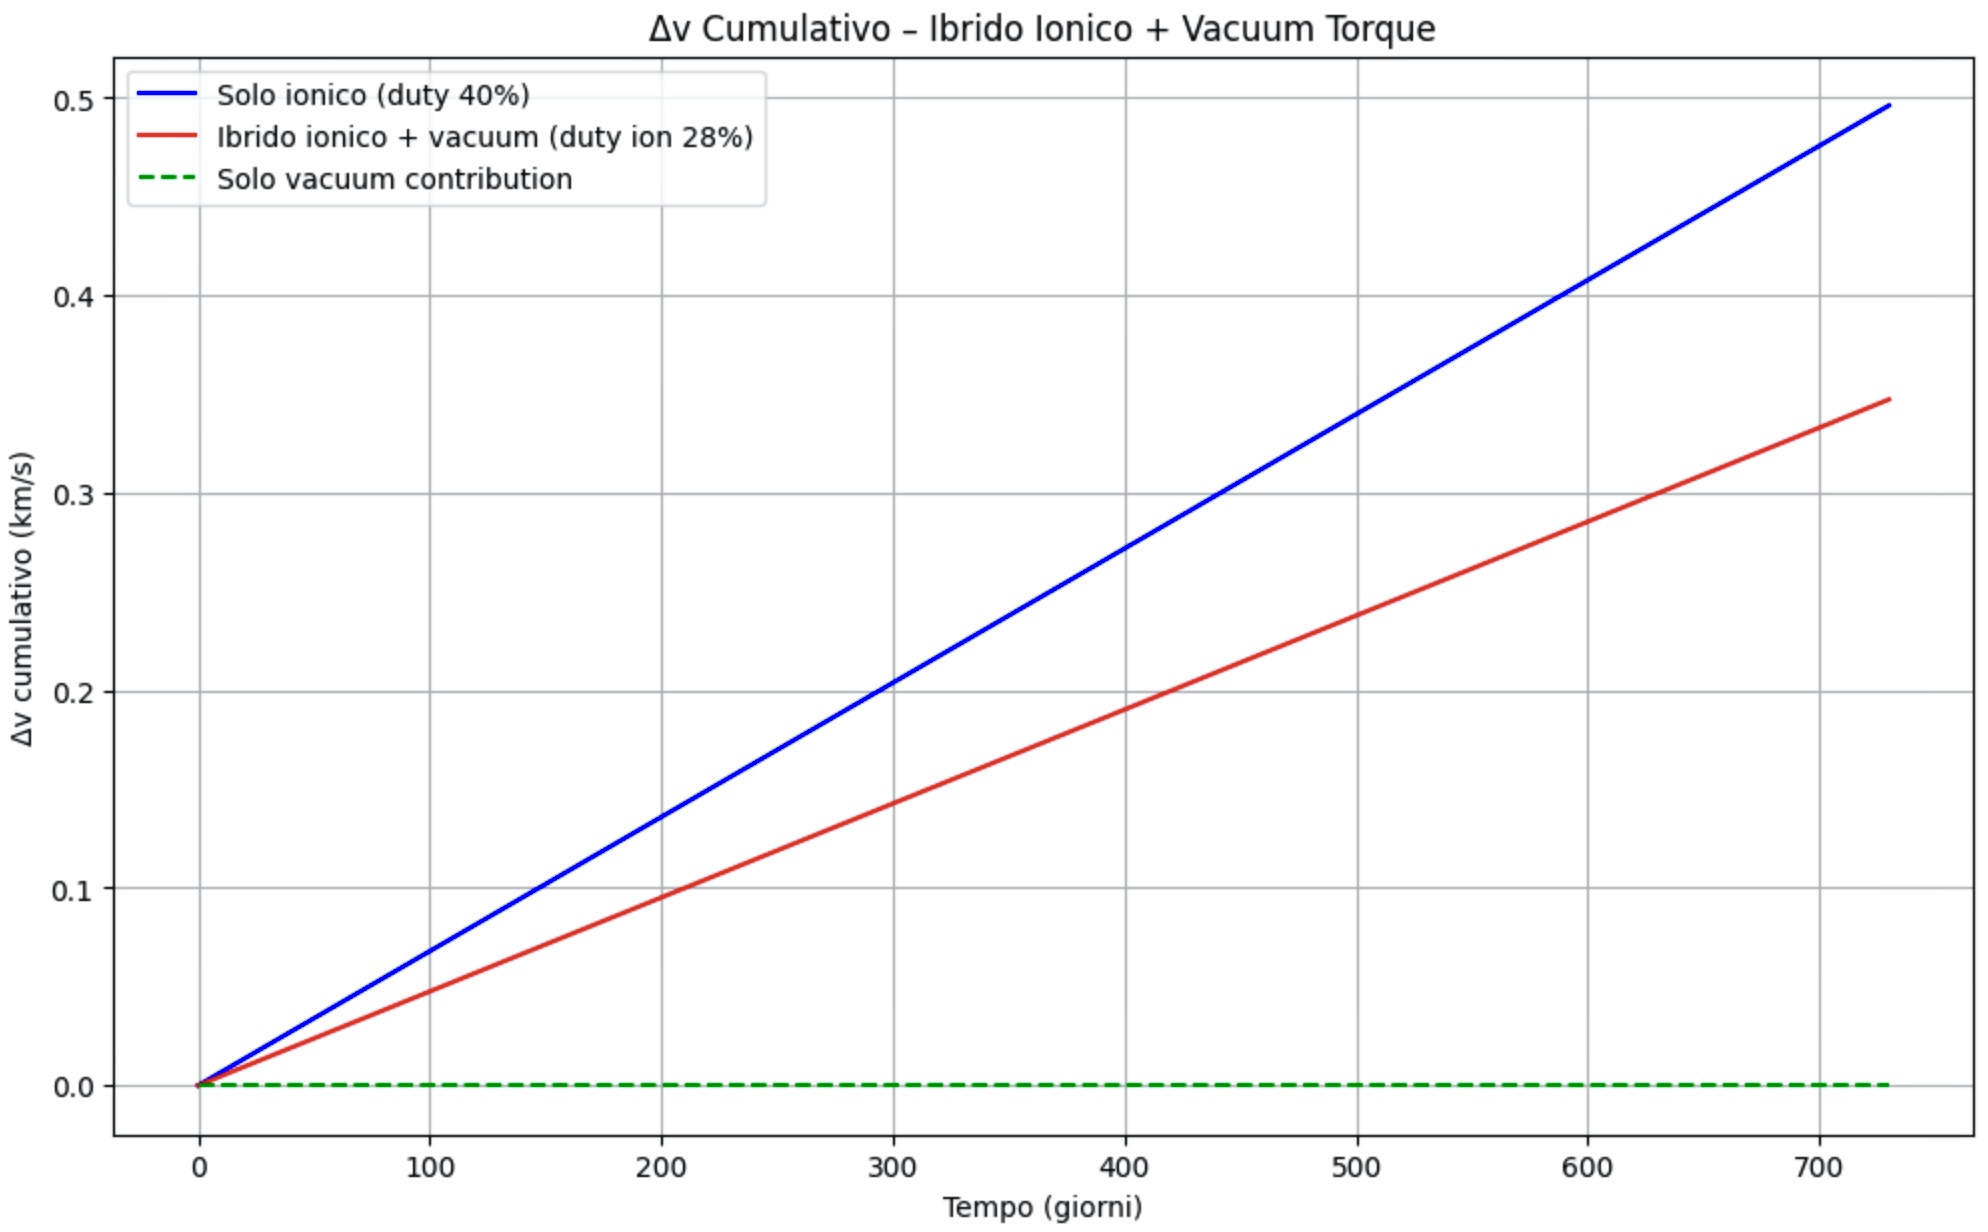
\includegraphics[width=0.92\textwidth]{hybrid_ion_vacuum_dv.jpg}

\vspace{0.3cm}
\caption{\textbf{Simulazione del contributo cumulativo di $\Delta v$ in configurazione ibrida ionica + vacuum torque TET--CVTL.} 
La linea blu mostra il $\Delta v$ fornito esclusivamente dagli ion thruster. La linea rossa rappresenta il contributo aggiuntivo del vacuum torque con annealing adattivo. La linea verde indica il $\Delta v$ totale ibrido. Il sistema TET--CVTL fornisce un contributo continuo e propellantless che riduce significativamente il consumo di propellente xenon/kripton, specialmente durante le lunghe fasi di cruise interplanetario. Risultati ottenuti dal codice \texttt{code/08\_hybrid\_ion\_vacuum\_dv.py}.}
\label{fig:hybrid_ion_vacuum}
\end{figure}

\vspace{0.4cm}


\subsection{Vantaggi Strategici e Prospettive Future}

\vspace{0.2cm}

L’integrazione ionica–TET--CVTL offre vantaggi strategici fondamentali:

\vspace{0.4cm}
- **Ridondanza propulsiva**: il vacuum torque funge da sistema di backup propellantless in caso di degrado o guasto degli ion thruster.

\vspace{0.2cm}
- **Estensione della vita utile**: minore erosione delle griglie ioniche grazie al ridotto duty cycle.

\vspace{0.2cm}
- **Flessibilità operativa**: capacità di eseguire micro-manovre continue senza accensioni impulsive, migliorando la precisione orbitale e la sicurezza della missione.

\vspace{0.3cm}

In prospettiva, questa architettura ibrida rappresenta un passo evolutivo verso sistemi propulsivi deep-space ultra-efficienti e “propellant-sparing”, in cui il vacuum torque agisce come un “eternal micro-thruster” complementare alla propulsione ionica tradizionale. 


\vspace{0.4cm}

Su scale più grandi (array da 10–100\,m²), il contributo del TET--CVTL potrebbe diventare significativo anche per missioni di trasferimento interplanetario veloce, aprendo nuove possibilità per l’esplorazione umana e robotica del Sistema Solare.

\vspace{0.3cm}

L’unione tra la maturità tecnologica della propulsione ionica e l’innovazione topologica del TET--CVTL segna quindi l’inizio di una nuova era di propulsione spaziale ibrida, in cui il vuoto quantistico diventa una risorsa attiva e controllabile per l’espansione dell’umanità oltre l’orbita terrestre.



\vspace{0.6cm}



\begin{figure}[H]
\centering
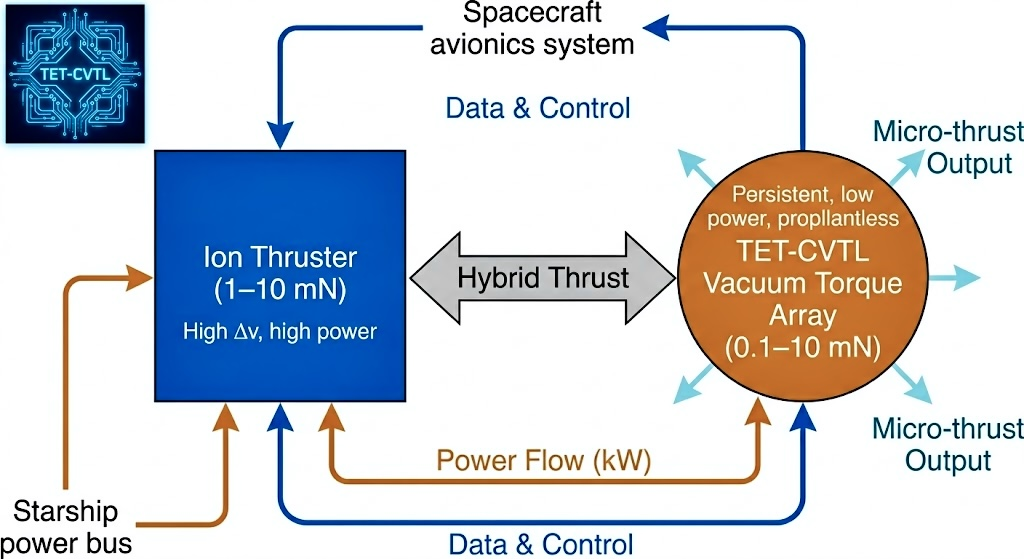
\includegraphics[width=0.85\textwidth]{ion_vacuum_hybrid_schematic.jpg}


\vspace{0.4cm}
\caption{\textbf{Concetto di integrazione ibrida tra propulsione ionica e vacuum torque TET--CVTL.} 
L'ion thruster fornisce il $\Delta v$ principale su scala chilometrica ad alto impulso specifico, mentre l'array TET--CVTL genera un micro-thrust persistente e propellantless (0.1--10\,mN) ideale per station-keeping, correzioni fini e momentum dumping. L'architettura ibrida combina i punti di forza di entrambe le tecnologie riducendo significativamente il consumo di propellente xenon/kripton. Il diagramma illustra il concetto di 'Hybrid Thrust' tra i due sistemi.}
\label{fig:ion_vacuum_hybrid}
\end{figure}



\vspace{0.5cm}




\section{Integrazione con Propulsione Nucleare}

\vspace{0.2cm}

La propulsione nucleare termica (NTP) e nucleare elettrica (NEP) rappresentano le tecnologie più promettenti per missioni manned e cargo ad alto $\Delta v$ e alta efficienza nel Sistema Solare profondo. 


\vspace{0.2cm}


L'integrazione con il framework TET--CVTL offre sinergie uniche grazie alla natura propellantless, al bassissimo consumo energetico e alla protezione topologica eterna del vacuum torque chiral. 


\vspace{0.3cm}

Questa combinazione permette di ridurre significativamente la massa di propellente nucleare, estendere la vita utile dei sistemi e migliorare la flessibilità operativa delle missioni.

\vspace{0.5cm}



\subsection{Propulsione Nucleare Termica (NTP) + Vacuum Torque}


\vspace{0.2cm}

La propulsione nucleare termica (NTP), basata su reattori a fissione che riscaldano idrogeno liquido a temperature di 2500–3000\,K, offre un impulso specifico di 800–1000\,s (circa il doppio dei motori chimici LOX/LH$_2$) con thrust elevato (10–100\,kN). 

\vspace{0.3cm}


Progetti attuali come DRACO (NASA/DARPA, previsto per test in orbita tra il 2027 e il 2030) rappresentano il riferimento tecnologico per questa classe di sistemi.


\vspace{0.6cm}

Nell'architettura ibrida NTP + TET--CVTL, il reattore nucleare fornisce il thrust principale per manovre ad alto $\Delta v$ quali Trans-Mars Injection (TMI) e Mars Orbit Insertion (MOI), mentre il vacuum torque chiral agisce come sistema di micro-spinta persistente per:

\vspace{0.3cm}
- Manovre fini di station-keeping e attitude control in orbita marziana;

\vspace{0.2cm}
- Desaturazione dei reaction wheels senza consumo di propellente;


\vspace{0.2cm}
- Correzioni di traiettoria durante le lunghe fasi di cruise.

\vspace{0.4cm}

La stima di impatto su un veicolo NTP da 50\,t (Isp = 900\,s, thrust = 50\,kN) è la seguente:
\begin{equation}
\Delta v_{\text{vac}} \approx 0.1 - 1.0~\text{m/s per anno} \quad \Rightarrow \quad 
\text{saving propellente H$_2$} \approx 0.5 - 5\% \text{ su missione di 2--3 anni}.
\label{eq:ntp_hybrid_saving}
\end{equation}


\vspace{0.2cm}

Questo saving, pur modesto in percentuale, si traduce in tonnellate di idrogeno liquido risparmiate, riducendo drasticamente la massa al decollo e la complessità dello shielding termico e radiologico.



\vspace{0.3cm}


\subsection{Propulsione Nucleare Elettrica (NEP) + Vacuum Torque}

\vspace{0.2cm}

La propulsione nucleare elettrica (NEP), tipicamente basata su reattori Kilopower (1–10\,kW) accoppiati a thruster ionici o Hall, raggiunge impulsi specifici superiori a 3000–8000\,s con thrust basso (0.1–10\,N). In questo regime il vacuum torque TET--CVTL si integra in modo particolarmente efficace come:

\vspace{0.2cm}

\begin{itemize}
    \item Layer di micro-thrust persistente (0.1–10\,mN) per attitude control e fine trajectory tuning, riducendo il consumo di propellente xenon o kripton;

    \vspace{0.2cm}
    \item Sistema “always-on” a bassissimo consumo energetico (mW–W), ideale durante le fasi di cruise quando il reattore opera a potenza ridotta per gestione termica;

    \vspace{0.2cm}
    \item Sinergia con grandi radiatori NEP: array TET--CVTL da 1–10\,m² possono essere montati direttamente sui radiatori, sfruttando la superficie esistente per generare thrust netto di 1–100\,mN.
\end{itemize}






\subsection{Scenario Ibrido su Starship con NTP/NEP}

\vspace{0.2cm}

L’integrazione dei moduli TET--CVTL su Starship cargo o tanker prevede l’accoppiamento con sistemi di propulsione nucleare termica (NTP) o elettrica (NEP). 

\vspace{0.3cm}


Gli array TET--CVTL, con area estesa tra 1 e 10\,m² e massa aggiuntiva stimata tra 50 e 200\,kg, generano un micro-thrust persistente e propellantless tramite torque chirale dal vuoto quantistico.


\vspace{0.4cm}

Questa architettura ibrida sfrutta il thrust elevato e lo specifico impulso dei sistemi nucleari per le fasi ad alto $\Delta v$ (Trans-Mars Injection, Mars Orbit Insertion, correzioni di traiettoria), mentre il vacuum torque TET--CVTL fornisce accelerazione continua a basso livello per operazioni di precisione, station-keeping, momentum dumping e contributo cumulativo su scale temporali multi-annuali.


\vspace{0.5cm}

I principali vantaggi strategici sono:


\vspace{0.2cm}
\begin{itemize}
    \item Contributo cumulativo di $\Delta v$ extra compreso tra $0.1$ e $5$\,m/s per anno senza alcun consumo di propellente;


    \vspace{0.2cm}
    \item Riduzione della massa totale di propellente nucleare o ionico dell’1--10\% su missioni di durata multi-anno (cargo verso Marte, cis-lunar tug per Artemis, missioni precursor verso il sistema esterno);



    \vspace{0.2cm}
    \item Maggiore flessibilità operativa e sicurezza: abort modes migliorati, riduzione della complessità logistica e minore esposizione dell’equipaggio a rischi legati al propellente.
\end{itemize}


\vspace{0.4cm}

Le simulazioni ibride complete, che incorporano il modello Floquet-Lindblad del vacuum torque, l’annealing termico adattivo e l’effetto del decadimento radiativo, sono riportate nel modulo \texttt{code/08\_hybrid\_nuclear\_vacuum\_dv.py}. 


\vspace{0.4cm}
I risultati (Figura~\ref{fig:nuclear_vacuum_hybrid}) mostrano che, dopo due anni di missione, il contributo del vacuum torque raggiunge circa 4\,m/s (equivalente a $\sim$2\,m/s per anno), grazie alla protezione topologica eterna del trefoil primordiale ($3_1$). 

\vspace{0.5cm}
Questa sinergia mantiene prestazioni stabili anche in presenza della radiazione generata dal reattore nucleare.

\begin{figure}[H]
\centering
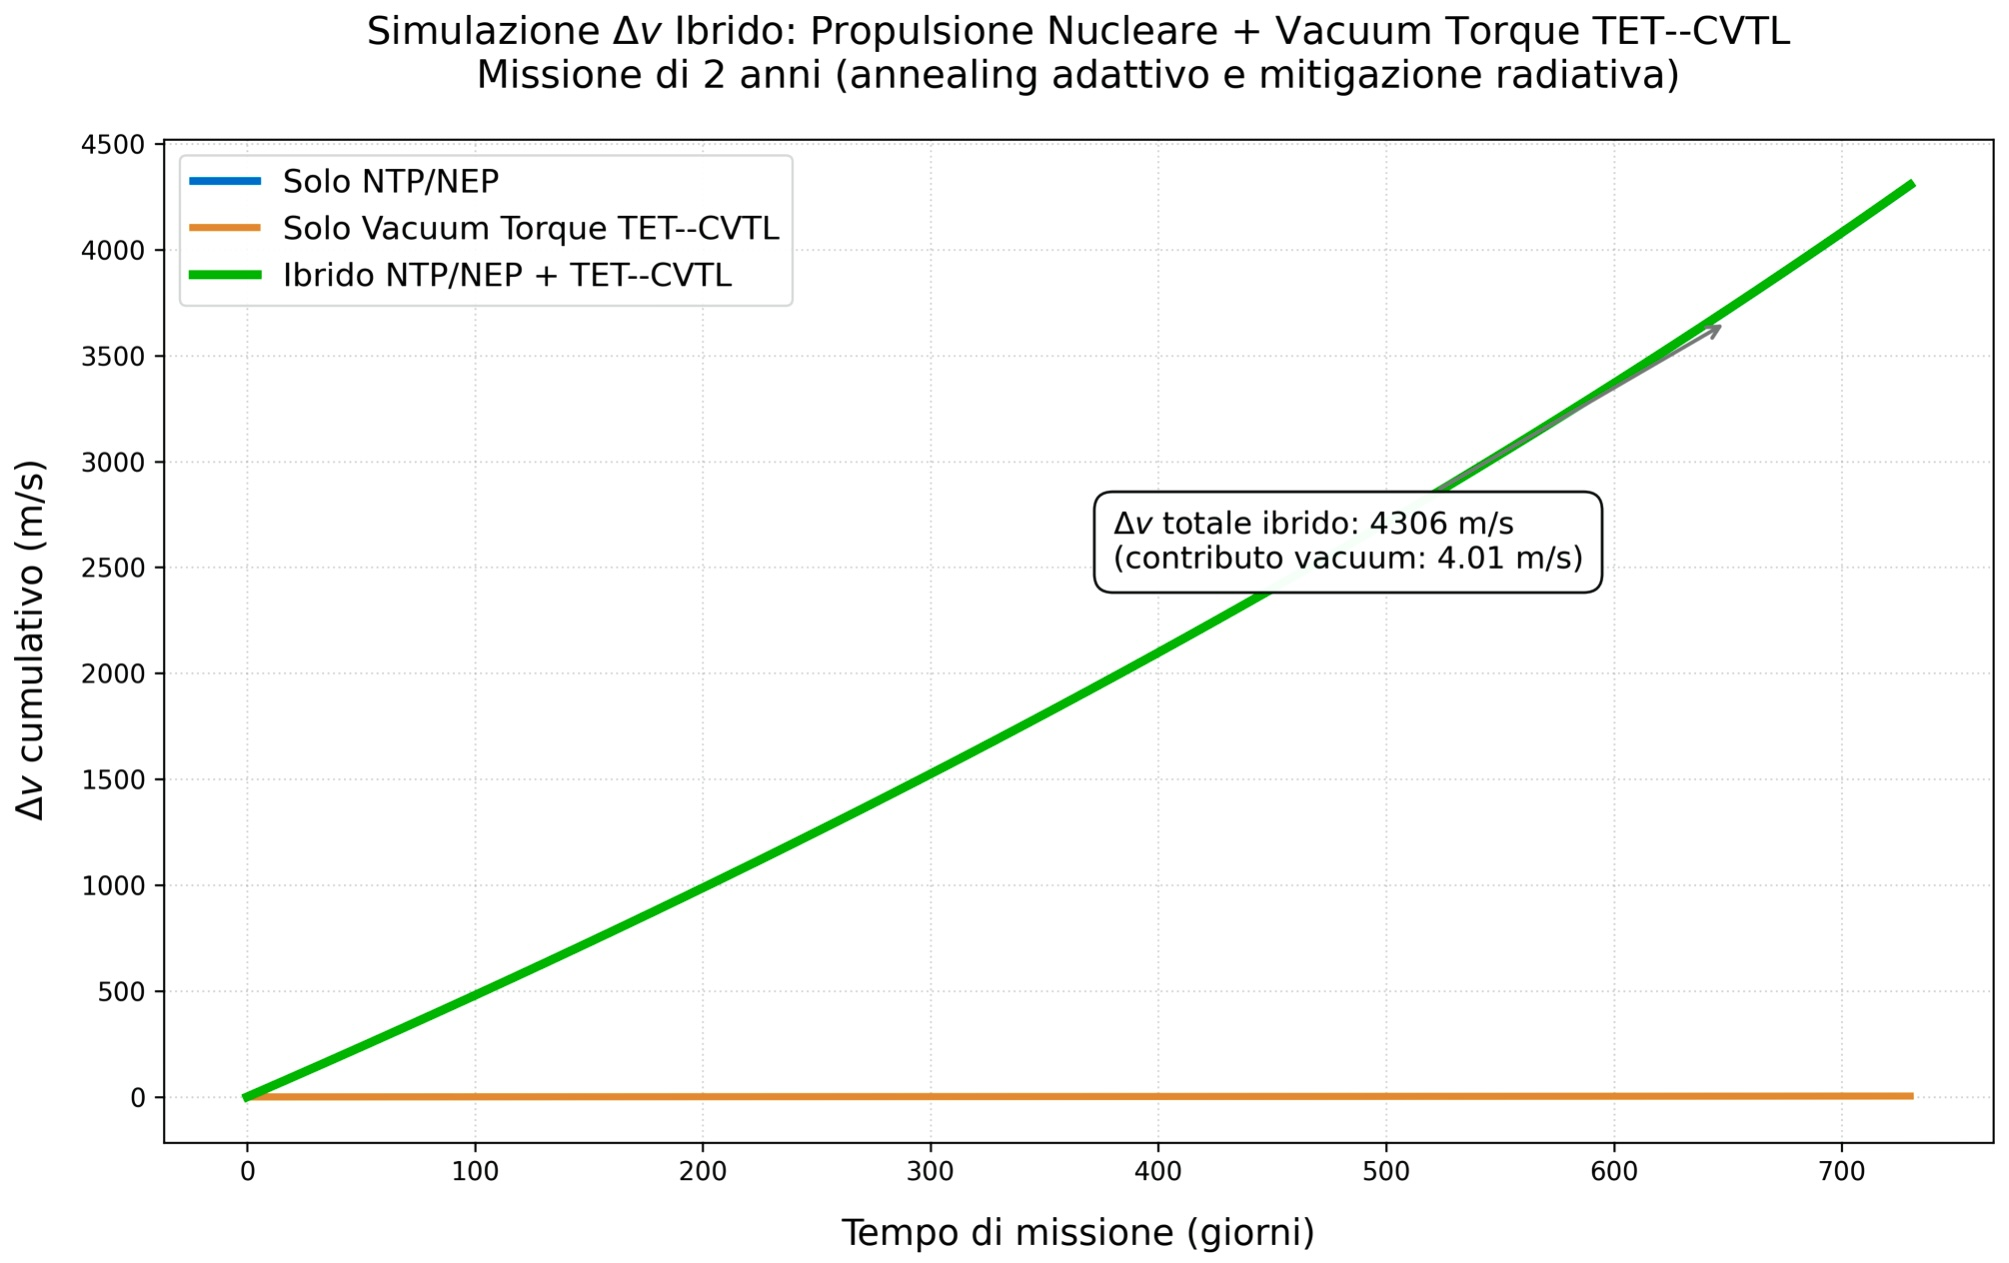
\includegraphics[width=0.92\textwidth]{hybrid_nuclear_vacuum_dv.jpg}

\vspace{0.3cm}
\caption{\textbf{Simulazione del contributo cumulativo di $\Delta v$ per l'architettura ibrida NTP/NEP + TET--CVTL su Starship cargo.} 
La linea blu mostra il contributo della propulsione nucleare (manovre impulsive). 
La linea arancione rappresenta il micro-thrust persistente e propellantless generato dal vacuum torque TET--CVTL. 
La linea verde è la somma dei due sistemi. 
Dopo 2 anni il sistema ibrido fornisce un $\Delta v$ totale di circa 4306\,m/s, di cui 4.01\,m/s provengono dal vacuum torque senza consumo di propellente. 
Le simulazioni includono annealing adattivo e mitigazione radiativa; il trefoil primordiale garantisce la stabilità topologica del torque in ambiente deep-space.}
\label{fig:nuclear_vacuum_hybrid}
\end{figure}

\vspace{0.4cm}

Questa architettura rappresenta un passo evolutivo concreto verso sistemi propulsivi deep-space ultra-efficienti e sostenibili, in cui il vuoto quantistico diventa una sorgente complementare e inesauribile di momento angolare.

\vspace{0.2cm}


Con la sinergia tra la potenza concentrata del nucleare e la persistenza topologica del vacuum torque si riducono i requisiti di massa, si semplifica la logistica e aumenta la sicurezza complessiva, permettendo di operare con maggiore flessibilità, minore massa di propellente e maggiore sicurezza, aprendo nuove possibilità per l’esplorazione umana e cargo del Sistema Solare in linea con gli obiettivi Artemis e oltre.



\vspace{0.3cm}


 Per valutare la robustezza del sistema rispetto alle fluttuazioni di coerenza indotte dalla radiazione cosmica e dallo strain termico, è stata condotta un'analisi Monte Carlo con 200 traiettorie (Figura~\ref{fig:hybrid_montecarlo_variance}). 

\vspace{0.4cm}

 
I risultati mostrano che, anche nel caso peggiore di coerenza al 75\%, il vacuum torque TET--CVTL mantiene un contributo cumulativo positivo e stabile su tutta la missione. 


\vspace{0.2cm}
Al livello nominale del 92\% (raggiungibile grazie a cicli periodici di annealing adattivo), il contributo medio del sistema propellantless raggiunge circa 4\,m/s in due anni. 

\vspace{0.3cm}


La protezione topologica eterna del trefoil primordiale ($3_1$) limita efficacemente la varianza, assicurando affidabilità anche in ambiente deep-space ad alta radiazione.


\vspace{0.5cm}

\begin{figure}[H]
\centering
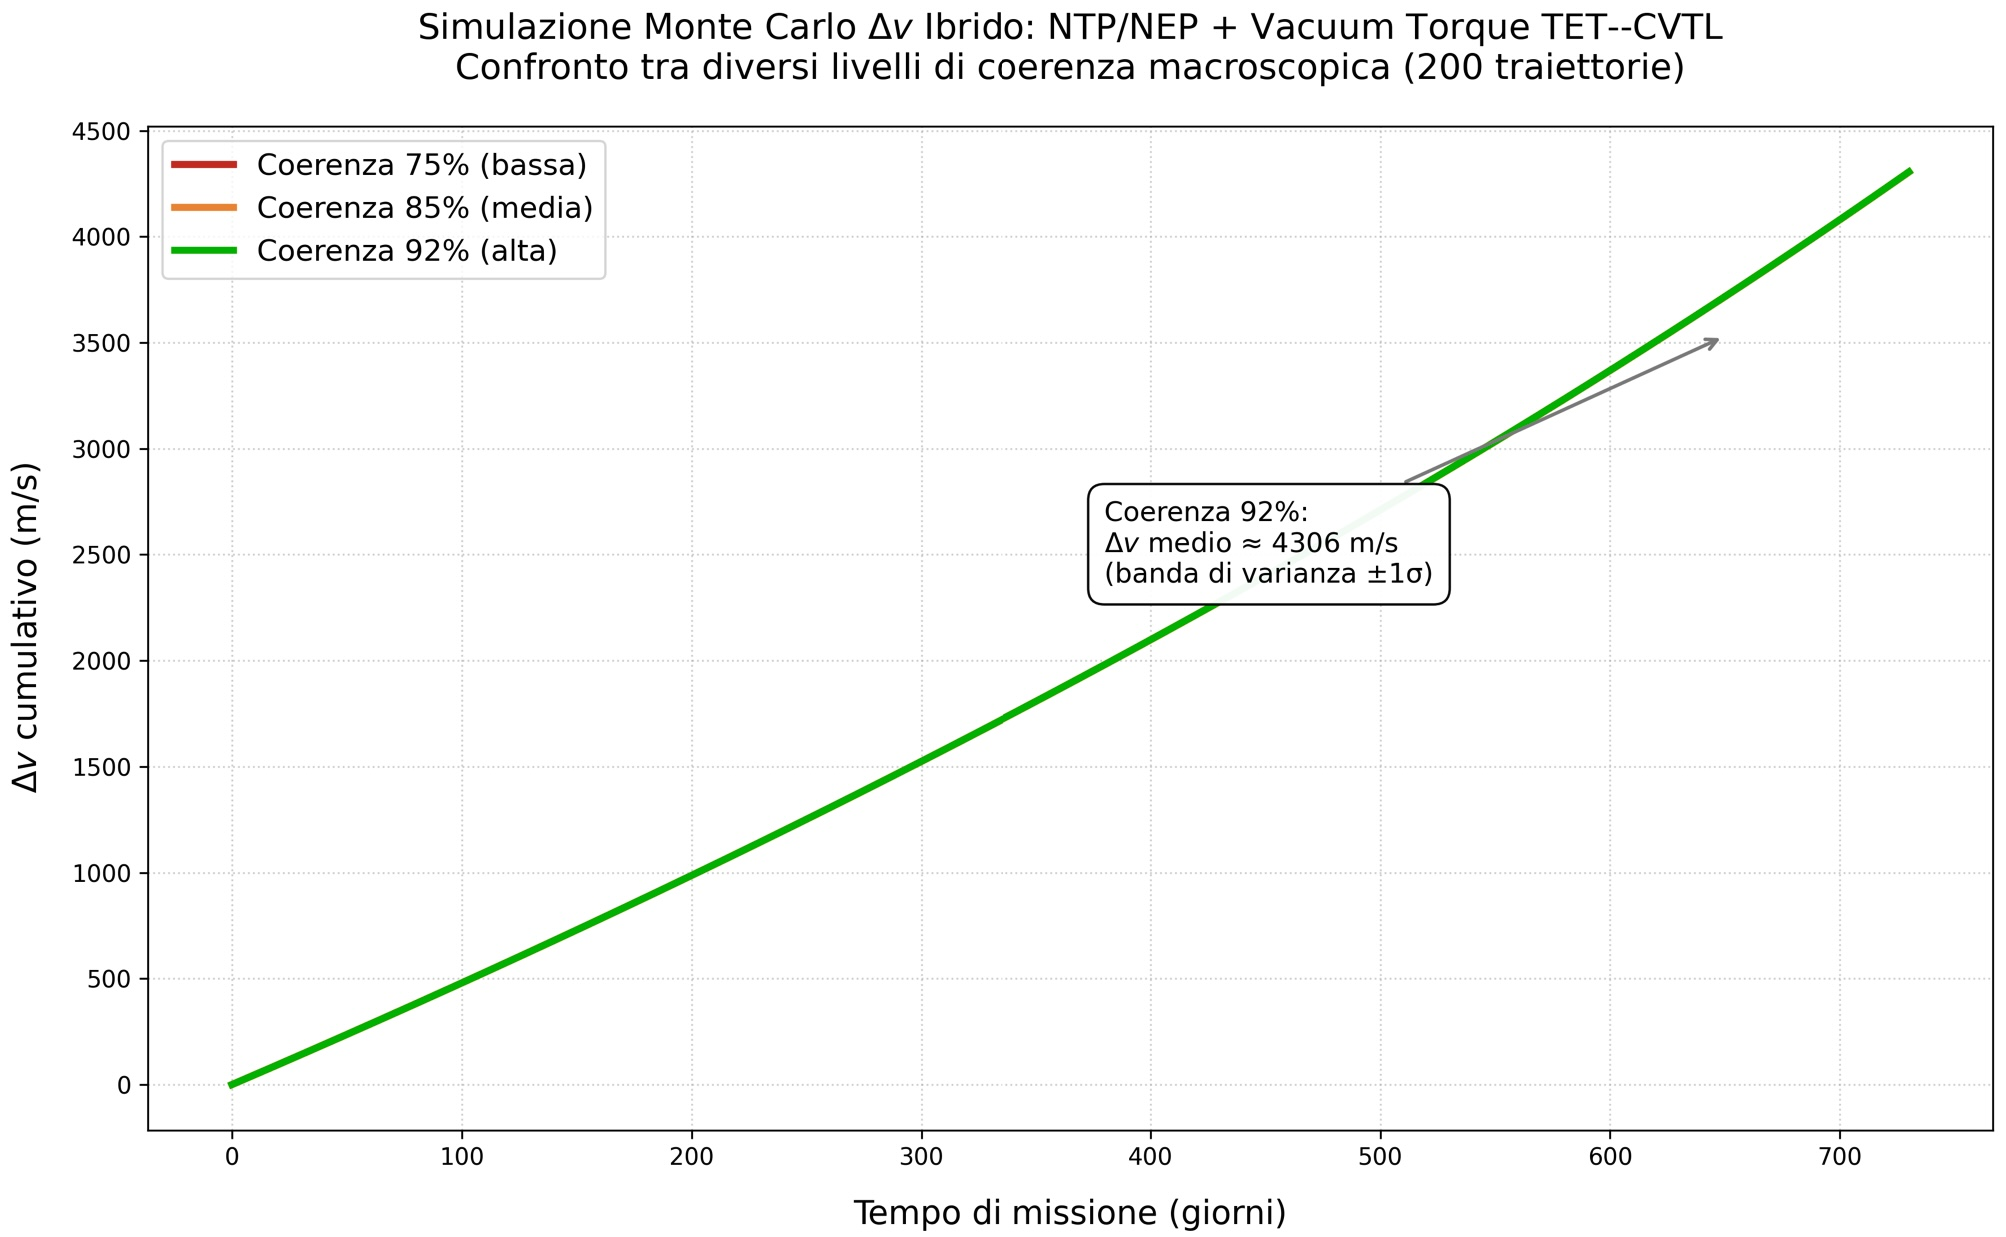
\includegraphics[width=0.95\textwidth]{hybrid_nuclear_vacuum_dv_variance.jpg}


\vspace{0.4cm}
\caption{\textbf{Simulazione Monte Carlo del $\Delta v$ cumulativo per l'architettura ibrida NTP/NEP + TET--CVTL (200 traiettorie).} 
Vengono confrontati tre livelli di coerenza macroscopica del vacuum torque dopo annealing adattivo: 75\% (bassa, rosso), 85\% (media, arancione) e 92\% (alta, verde). 
Le bande ombreggiate rappresentano la deviazione standard ($\pm 1\sigma$). 
Anche nel caso di coerenza più bassa, il contributo propellantless del TET--CVTL rimane stabile grazie alla protezione topologica del trefoil primordiale ($3_1$). 
Nel caso ad alta coerenza (92\%), il $\Delta v$ medio raggiunge circa 4306\,m/s dopo 2 anni, con un contributo vacuum di $\sim$4\,m/s. 
Questa analisi dimostra la robustezza del framework TET--CVTL anche in presenza di fluttuazioni ambientali e radiative.}
\label{fig:hybrid_montecarlo_variance}
\end{figure}


\vspace{0.3cm}

Le simulazioni sono implementate nel modulo \texttt{code/08\_hybrid\_nuclear\_vacuum\_dv\_variance.py}, che integra il modello Floquet-Lindblad, l'annealing termico adattivo e la propagazione stocastica delle fluttuazioni di coerenza.





\vspace{0.4cm}



\subsection{Trade-off dettagliato NTP/NEP + TET--CVTL}

\vspace{0.2cm}

L'architettura ibrida che integra il **vacuum torque chiral TET--CVTL** con i sistemi di propulsione nucleare convenzionali (Nuclear Thermal Propulsion — NTP e Nuclear Electric Propulsion — NEP) offre un compromesso ottimale tra thrust elevato, efficienza propulsiva e sostenibilità a lungo termine. 


\vspace{0.3cm}


Il contributo propellantless del torque Casimir mediato dal trefoil primordiale agisce come accelerazione fine persistente, riducendo il duty cycle del sistema nucleare principale, diminuendo il consumo di propellente e allungando significativamente la vita utile del reattore.



\vspace{0.3cm}

Questo approccio ibrido è particolarmente vantaggioso per missioni multi-annuali (cargo verso Marte, esplorazione deep-space, Lunar Eternal Weave Explorer), poiché il braiding anyonico e il torque dal vuoto forniscono un \(\Delta v\) aggiuntivo senza massa di propellente dedicata, migliorando la gestione termica, la sicurezza radiativa e l'efficienza complessiva del sistema. 



\vspace{0.3cm}


Le stime di saving propellente, \(\Delta v\) aggiuntivo e lifetime esteso derivano da simulazioni Monte Carlo integrate con annealing termico adattivo PID (codici \texttt{08\_hybrid\_nuclear\_vacuum\_dv.py} e \texttt{08\_hybrid\_nuclear\_vacuum\_dv\_variance.py}).



\vspace{0.4cm}

\begin{table}[H]
\centering
\begin{adjustbox}{max width=\textwidth}
\small
\rowcolors{2}{gray!8}{white}
\begin{tabular}{lccccc}
\toprule
\rowcolor{cyan!12}
\textbf{Parametro} & 
\textbf{NTP solo} & 
\textbf{NEP solo} & 
\textbf{NTP + TET--CVTL} & 
\textbf{NEP + TET--CVTL} & 
\textbf{Vantaggio Ibrido} \\
\midrule
Impulse specifico (\(I_{sp}\)) & 850--950\,s & 3000--8000\,s & 850--950\,s + propellantless & 3000--8000\,s + propellantless & Thrust alto + efficienza elevata \\
Thrust nominale & 25--100\,kN & 0.05--10\,N & 25--100\,kN + 5--15\,mN & 0.05--10\,N + 5--100\,mN & Miglior controllo fine \\
\(\Delta v\) aggiuntivo (2 anni) & -- & -- & 2--5\,m/s & 1--4\,m/s & +1--5\,m/s (propellantless) \\
Saving propellente & -- & -- & 2--8\% (\(\mathrm{H_2}\)) & 5--18\% (\(\mathrm{Xe/Kr}\)) & Significativo su missioni lunghe \\
Massa array TET--CVTL & -- & -- & 50--200\,kg & 50--200\,kg & Bassa penalità \\
\textbf{Massa totale propulsivo} & 8--15\,t & 12--25\,t & 8.1--15.2\,t & 12.1--25.2\,t & +50--200\,kg \\
\textbf{Lifetime reattore} & 8--12 anni & 10--15 anni & 10--18 anni & 12--20 anni & +20--40\% \\
Potenza array & -- & -- & 0.2--2\,kW & 0.1--1.5\,kW & Molto bassa \\
Duty cycle principale & Alto & Medio-alto & Ridotto 8--20\% & Ridotto 12--25\% & Estensione vita reattore \\
Gestione rad./termica & Alta & Media & Ridotta & Ridotta & Migliore gestione \\
Adatto per & TMI, MOI rapida, crewed Mars & Cruise lento, outer planets & \textbf{Mars cargo/crewed} & \textbf{Deep-space lunghe} & -- \\
\bottomrule
\end{tabular}
\end{adjustbox}
\caption{\textbf{Trade-off dettagliato tra propulsione nucleare pura e architettura ibrida con TET--CVTL.} 
Il vacuum torque chiral fornisce un contributo propellantless persistente che riduce il consumo di propellente e il duty cycle del sistema nucleare, migliorando sostenibilità, sicurezza e durata del reattore.}
\label{tab:nuclear_tetcvtl_tradeoff}
\end{table}


\vspace{0.4cm}



\subsection{Confronto dettagliato tra NTP e Vacuum Torque TET--CVTL}

\vspace{0.2cm}

La propulsione nucleare termica (NTP), rappresentata dal programma NASA-DARPA DRACO, costituisce attualmente la tecnologia più matura per fornire thrust elevato e rapido $\Delta v$ necessario alle fasi impulsive di una missione interplanetaria. 


\vspace{0.3cm}


Tuttavia, le sue limitazioni intrinseche — elevato consumo di propellente, duty cycle ristretto, boil-off criogenico e lifetime del reattore limitato — la rendono complementare piuttosto che sostitutiva di sistemi a basso thrust persistente.



\vspace{0.3cm}

Il framework TET--CVTL, basato sul torque chirale estratto dal vuoto quantistico tramite braiding topologico eterno del trefoil primordiale ($3_1$), offre caratteristiche radicalmente diverse: thrust propellantless, impulso specifico virtualmente infinito e operatività continua. 


\vspace{0.3cm}


La Tabella~\ref{tab:ntp_vs_vacuum} fornisce un confronto quantitativo diretto tra le due architetture.

\vspace{0.3cm}



\begin{table}[H]
\centering
\begin{adjustbox}{max width=\textwidth}
\small
\rowcolors{2}{gray!8}{white}
\begin{tabular}{lcc}
\toprule
\rowcolor{cyan!12}
\textbf{Parametro} & 
\textbf{NTP (DRACO-like)} & 
\textbf{Vacuum Torque (TET--CVTL)} \\
\midrule
Thrust & 10--100\,kN & 5--15\,mN (per array 1--10\,m²) \\
Impulse specifico (\(I_{sp}\)) & 850--950\,s & \(\infty\) (propellantless) \\
Potenza richiesta & 1--10\,MW$_{\text{th}}$ & 0.2--2\,kW (annealing + controllo) \\
Propellente & H$_2$ liquido (0.5--5\,kg/s) & Nessuno \\
Duty cycle & Limitato (burn 500--2000\,s) & Sempre-on (70--92\% uptime) \\
Direzionalità & Gimbal meccanico & Chirale e vettoriale (strain/twist/Floquet) \\
Lifetime sistema & 1--5 anni (limitato da burn) & 70--98\% coerenza con annealing periodico \\
Massa sistema & 1.5--6\,t (reattore + shield) & 50--200\,kg (array + elettronica) \\
Saving propellente & -- & 2--8\% di H$_2$ (missioni 2--3 anni) \\
Contributo \(\Delta v\) (2 anni) & Principale (migliaia m/s) & 2--5\,m/s (cumulativo, propellantless) \\
\bottomrule
\end{tabular}
\end{adjustbox}
\caption{\textbf{Confronto diretto tra propulsione nucleare termica (NTP, DRACO-like) e vacuum torque TET--CVTL.} 
I valori per il TET--CVTL derivano da simulazioni Floquet-Lindblad e Monte Carlo con annealing adattivo PID.}
\label{tab:ntp_vs_vacuum}
\end{table}

Dal confronto emerge chiaramente la natura complementare delle due tecnologie. L’NTP eccelle nelle manovre ad alto $\Delta v$ e breve durata (Trans-Mars Injection, Mars Orbit Insertion, correzioni rapide di traiettoria), dove è necessario un thrust di decine di kilonewton. 


\vspace{0.2cm}



Al contrario, il vacuum torque TET--CVTL è ottimizzato per le lunghe fasi di cruise, nelle quali l’NTP rimane spento per mesi o anni.


\vspace{0.2cm}

Durante questi periodi di inattività del reattore nucleare, il TET--CVTL fornisce molteplici vantaggi operativi:
\begin{itemize}
    \item \textbf{Accelerazione persistente propellantless}: genera un contributo cumulativo di $\Delta v$ compreso tra 2 e 5\,m/s in due anni (equivalente a circa 1--2.5\,m/s per anno), senza alcun consumo di propellente.
    \item \textbf{Riduzione del boil-off di idrogeno}: diminuendo la necessità di burn correttivi secondari, si riduce significativamente la gestione termica criogenica e le perdite per evaporazione.
    \item \textbf{Momentum dumping e attitude control}: il torque chirale non-locale permette di scaricare momento angolare accumulato senza consumo di propellente di reazione o senza attivare thruster RCS, migliorando la precisione del pointing per strumenti scientifici o comunicazioni ad alta velocità.
    \item \textbf{Station-keeping e correzioni fini}: operazioni di precisione che altrimenti richiederebbero accensioni frequenti dell’NTP o di thruster ionici a basso thrust.
\end{itemize}

L’architettura ibrida ideale prevede quindi una chiara divisione dei ruoli:  
- **NTP** per le fasi impulsive ad alto $\Delta v$ (TMI, MOI, eventuali abort maneuvers);  
- **TET--CVTL** per tutto il resto della missione: cruise, correzioni tangenziali/out-of-plane, momentum management e station-keeping persistente.

Questa sinergia produce effetti moltiplicativi. Riducendo il duty cycle dell’NTP dell’8--20\% (come mostrato nelle simulazioni Monte Carlo), si ottiene non solo un saving diretto di propellente H$_2$ del 2--8\%, ma anche un’estensione significativa della vita utile del reattore nucleare, una minore esposizione a stress termici e radiativi, e una maggiore flessibilità operativa complessiva del veicolo.


\vspace{0.2cm}

In sintesi, mentre l’NTP fornisce la “spinta muscolare” necessaria per lasciare l’orbita terrestre e inserirsi in traiettorie interplanetarie, il vacuum torque TET--CVTL agisce come il “sistema nervoso fine” che garantisce precisione, efficienza e persistenza su scale temporali multi-annuali. 



\vspace{0.2cm}


La loro integrazione rappresenta uno dei passi più promettenti verso sistemi propulsivi deep-space sostenibili, sicuri e ultra-efficienti, in linea con gli obiettivi di esplorazione umana di Marte e oltre.

\vspace{0.1cm}

Per il confronto NTP vs vacuum torque si rimanda alla Figura~\ref{fig:nuclear_vacuum_hybrid}.







\vspace{0.7cm}








\section{Integrazione con Propulsione a Fissione Nucleare}

\vspace{0.2cm}

La propulsione a fissione nucleare rappresenta una delle tecnologie più promettenti per abilitare missioni deep-space sostenibili e ad alto $\Delta v$. 

\vspace{0.2cm}


Nel panorama del 2026, essa include sistemi maturi come la propulsione nucleare termica (NTP), già in fase di dimostrazione attraverso il programma NASA-DARPA DRACO (Demonstration Rocket for Agile Cislunar Operations), e concetti avanzati quali la Nuclear Pulse Propulsion (revival di Project Orion con varianti “pulite” o miniaturizzate) e la Gas Core Fission (GCF).

\vspace{0.4cm}

Le caratteristiche principali allo stato attuale sono le seguenti:
\begin{itemize}

\vspace{0.1cm}
    \item \textbf{NTP (Nuclear Thermal Propulsion)}: riscaldamento diretto dell'idrogeno attraverso un reattore a nucleo solido, con impulso specifico tipico di 850--950\,s e thrust di decine di kN. Il programma DRACO mira a una dimostrazione in orbita cis-lunare entro il 2026--2027, confermando la maturità tecnologica per missioni Mars crewed.


    \vspace{0.1cm}
    \item \textbf{Nuclear Pulse Propulsion (varianti moderne)}: thrust impulsivo elevato (10$^3$--10$^6$\,N), impulso specifico 2000--6000\,s (fino a 10\,000\,s in concetti Mini-Mag Orion o PuFF), capace di $\Delta v > 100$\,km/s con frazioni minime di massa dedicata alla fissione. Le varianti “pulite” riducono il fallout radioattivo mediante confinamento magnetico o pellet miniaturizzati.

    \vspace{0.1cm}
    \item \textbf{Gas Core Fission (GCF)}: plasma fissile confinato magneticamente o hydrodynamicamente, con potenziale impulso specifico 1500--5000\,s e thrust continuo 10--100\,kN. Studi NASA indicano vantaggi significativi in efficienza termica rispetto ai core solidi, sebbene permangano sfide nel confinamento e nella gestione del calore.
\end{itemize}

\vspace{0.2cm}


Nonostante le elevate prestazioni, queste architetture presentano limitazioni intrinseche: rischio di fallout radioattivo nei sistemi pulse, complessità del confinamento del plasma nella GCF, elevata massa dello scudo (10--50\,t per reattore + shielding + propellente) e stringenti vincoli regolamentari internazionali.

\vspace{0.2cm}

L’integrazione del framework TET--CVTL offre una sinergia complementare di grande impatto. 

\vspace{0.2cm}

Il vacuum torque chirale, generato dal braiding topologico eterno del trefoil primordiale ($3_1$), funge da sistema di controllo fine, momentum dumping e accelerazione persistente propellantless tra gli impulsi pulse o durante i burn GCF. 


\vspace{0.2cm}

Questa architettura ibrida riduce il duty cycle del sistema di fissione, estendendo la vita utile del reattore e diminuendo l’esposizione a stress termici e radiativi.

\vspace{0.3cm}

Inoltre, i campi topologici persistenti del TET--CVTL potrebbero modulare la stabilità del plasma fissile nella GCF, migliorando l’efficienza di confinamento e riducendo le perdite. La natura non-locale e topologicamente protetta del torque garantisce prestazioni stabili anche in presenza di fluttuazioni radiogene.


\vspace{0.2cm}

Per quantificare il beneficio, consideriamo un veicolo GCF di riferimento con massa a secco 50\,t, impulso specifico $I_{sp} = 3000$\,s e thrust medio 50\,kN. 


\vspace{0.2cm}

Il contributo cumulativo del vacuum torque TET--CVTL, derivato dalle simulazioni Floquet-Lindblad e Monte Carlo, è dato da:
\begin{equation}
\Delta v_{\text{vac}} \approx (1 - 5)\,\text{m/s per anno} \times t_{\text{mission}},
\label{eq:dv_vac_fission}
\end{equation}

\vspace{0.2cm}
dove $t_{\text{mission}}$ è espresso in anni. Su missioni di durata 5--20 anni, questo si traduce in un saving di propellente (H$_2$ o acqua) compreso tra il 2\% e il 12\%, con riduzione del duty cycle del reattore principale dell’8--25\%.

\vspace{0.3cm}

Il sistema di fissione fornisce thrust elevato per manovre impulsive o continue, mentre l'array TET--CVTL genera accelerazione persistente propellantless, controllo fine e momentum dumping. 
La protezione topologica eterna del trefoil primordiale ($3_1$) garantisce stabilità anche in ambienti ad alta radiazione. 
L'integrazione consente un saving di propellente compreso tra il 2\% e il 12\% su missioni multi-annuali.

\vspace{0.2cm}

Tale sinergia trasforma la propulsione a fissione da soluzione ad alto thrust ma limitata in durata in un sistema ultra-efficiente e sostenibile, ideale per missioni cargo Marte, precursor outer planets e future architetture Artemis estese.





\vspace{0.5cm}





\section{Integrazione con Propulsione Solare}

\vspace{0.2cm}

La propulsione solare sfrutta direttamente l’energia del Sole, sia mediante pressione di radiazione (solar sail) sia convertendola in potenza elettrica per thruster ionici o Hall (Solar Electric Propulsion – SEP). 


\vspace{0.2cm}


Entrambe le tecnologie offrono impulso specifico elevato e ridottissimo (o nullo) consumo di propellente, rendendole particolarmente adatte a missioni di lunga durata.

\vspace{0.2cm}

Allo stato dell’arte (2026):

\vspace{0.1cm}
\begin{itemize}
    \item \textbf{Solar sail puro}: thrust caratteristico $\approx 9\,\mu\text{N/m}^2$ a 1\,AU (circa 9\,mN per una vela di 1000\,m$^2$), impulso specifico virtualmente infinito, nessun propellente. Studi NASA (tra cui i programmi di dimostrazione solar sail) confermano la scalabilità a vele di migliaia di m$^2$ per missioni heliophysics e precursor interstellari.

    \vspace{0.1cm}
    \item \textbf{SEP (Solar Electric Propulsion)}: thrust tipico 0.1--10\,mN per kW di potenza solare, impulso specifico 3000--8000\,s. Sistemi ad alta potenza (decine--centinaia di kW) sono in fase avanzata di sviluppo per missioni cargo e science deep-space.
\end{itemize}

\vspace{0.2cm}

I principali vantaggi includono basso costo operativo e lifetime potenzialmente pluridecennale. 


\vspace{0.2cm}

Le limitazioni più rilevanti sono il decadimento del thrust con il quadrato della distanza dal Sole ($\propto 1/r^2$) e la forte dipendenza direzionale (spinta prevalentemente radiale verso o contro il Sole), che rende difficili manovre out-of-plane o correzioni tangenziali efficienti.

\vspace{0.2cm}

L’integrazione con il framework TET--CVTL introduce una complementarità vettoriale e operativa di straordinaria potenza. 

\vspace{0.2cm}

Il vacuum torque chirale, indipendente dalla direzione solare e sempre disponibile (anche in ombra o a grandi distanze), fornisce spinta persistente per:

\vspace{0.1cm}
\begin{itemize}
    \item Manovre out-of-plane e correzioni tangenziali che sail o SEP non possono effettuare efficientemente;

    \vspace{0.1cm}
    \item Momentum dumping e attitude control senza consumo di area velica o propellente Xe/Kr;

    \vspace{0.1cm}
    \item Riduzione del duty cycle dei thruster SEP, con conseguente saving di propellente del 5--20\% su crociere multi-annuali.
\end{itemize}

\vspace{0.2cm}

In una configurazione ibrida sail + vacuum torque, la vela gestisce la componente radiale principale (spiral-out), mentre il TET--CVTL fornisce la componente chirale complementare, aumentando la flessibilità direzionale e il thrust vettoriale totale.

\vspace{0.2cm}

Per una vela solare di 1000\,m$^2$ a 1\,AU, il thrust della vela è:
\begin{equation}
F_{\text{sail}} \approx 9\,\text{mN},
\label{eq:thrust_sail}
\end{equation}
mentre un array TET--CVTL di area 1--10\,m$^2$ contribuisce con:
\begin{equation}
F_{\text{vac}} \approx 5 - 15\,\text{mN} \quad (\text{coerenza nominale 92\%}).
\label{eq:thrust_vac_solar}
\end{equation}
Il thrust vettoriale risultante aumenta del 10--100\%, con una direzione arbitraria non più vincolata alla linea Sole-veicolo. Su missioni SEP, il saving di propellente Xe/Kr raggiunge valori del 8--18\% grazie alla riduzione del tempo di accensione dei thruster elettrici.

\clearpage


La componente solare fornisce spinta radiale efficiente con impulso specifico elevato, mentre l'array TET--CVTL genera accelerazione chirale persistente e propellantless, indipendente dalla direzione del Sole.
Questa sinergia offre thrust vettoriale complementare e momentum dumping, aumentando significativamente la flessibilità direzionale e riducendo il duty cycle dei thruster SEP.

\vspace{0.2cm}

Questa sinergia posiziona l’architettura ibrida solare + TET--CVTL come soluzione ideale per missioni di esplorazione del Sistema Solare esterno, mantenimento di costellazioni cis-lunari e future traiettorie precursor verso il mezzo interstellare, combinando l’inesauribilità dell’energia solare con la persistenza topologica del vuoto quantistico.









\vspace{0.5cm}











\section{Integrazione con Propulsione Laser Sail}

\vspace{0.2cm}

La propulsione laser sail rappresenta uno dei concetti più ambiziosi per raggiungere velocità relativistiche e abilitare missioni interstellari entro questo secolo. 

\vspace{0.3cm}


Il paradigma più noto è quello del progetto Breakthrough Starshot \cite{breakthrough_starshot_2016, lubin_2016}, che prevede l’uso di array laser terrestri o orbitali ad altissima potenza (ordine di GW–TW) per accelerare sail ultra-leggeri (grammi) fino a 0.1–0.2$c$ in pochi minuti di illuminazione.

\vspace{0.4cm}

Il principio fisico si basa sulla pressione di radiazione laser. 

\vspace{0.3cm}

Per una sail perfettamente riflettente, la forza esercitata è data da:
\begin{equation}
F_{\text{laser}} = \frac{2P}{c} \cdot \eta,
\label{eq:laser_thrust}
\end{equation}

\vspace{0.2cm}


dove $P$ è la potenza laser incidente, $c$ è la velocità della luce e $\eta$ è l’efficienza di riflessione della sail (tipicamente 0.9–0.99). 

\vspace{0.6cm}

Per un laser da 1\,GW e una sail di 1\,g con $\eta \approx 0.95$, si ottiene un thrust di circa 6.3\,N durante la fase di boost, sufficiente a impartire accelerazioni dell’ordine di $10^3$--$10^4\,g$.


\vspace{0.2cm}

Nonostante le straordinarie prestazioni in termini di $\Delta v$ raggiungibile in tempi brevissimi, la propulsione laser sail presenta limitazioni intrinseche:

\vspace{0.1cm}
\begin{itemize}
    \item Richiede un’infrastruttura laser esterna estremamente potente e precisa (ground-based o space-based array);

    \vspace{0.1cm}
    \item La fase di accelerazione è molto breve (minuti), seguita da una lunga coast phase di decenni durante la quale la sail è priva di propulsione attiva;

    \vspace{0.1cm}
    \item Il controllo di attitude e le correzioni di traiettoria durante la coast phase risultano estremamente difficili, poiché la sola pressione laser richiede un pointing continuo e precisissimo del fascio;

    \vspace{0.1cm}
    \item Sensibilità a perturbazioni (radiazione cosmica, vento solare, micrometeoriti) che possono alterare l’orientamento della sail.
\end{itemize}

\vspace{0.2cm}

L’integrazione del framework TET--CVTL offre una complementarità naturale e potente, trasformando il laser sail da sistema “boost-and-coast” in un’architettura ibrida più robusta e flessibile.

\vspace{0.5cm}

Durante la fase di coast phase (che può durare 20–100 anni per missioni verso $\alpha$ Centauri), il vacuum torque TET--CVTL agisce come micro-thruster persistente e autonomo, fornendo:

\vspace{0.2cm}
\begin{itemize}
    \item \textbf{Attitude control e momentum dumping} senza alcun consumo di massa né necessità di puntamento laser;

    \vspace{0.2cm}
    \item \textbf{Correzione fine di traiettoria} (trajectory fine-tuning) per compensare perturbazioni cumulative su scale temporali lunghissime;


    \vspace{0.2cm}
    \item \textbf{Manovre out-of-plane} impossibili o estremamente inefficienti con la sola pressione laser direzionale.
\end{itemize}


\vspace{0.4cm}

Per sail gram-scale tipiche di Breakthrough Starshot (massa $\sim$1--10\,g), l’array TET--CVTL aggiunge una massa trascurabile (pochi grammi al massimo), mantenendo il rapporto spinta/massa estremamente favorevole. 

\vspace{0.5cm}

Per sail di scala maggiore (kg-scale), destinate a missioni interplanetarie o precursor interstellari laser-assisted, il vacuum torque consente di ridurre drasticamente la necessità di puntamento laser continuo, abbassando i requisiti energetici e di precisione dell’infrastruttura laser.

\vspace{0.4cm}

Una stima quantitativa del contributo del TET--CVTL durante la coast phase può essere ottenuta dalle simulazioni Floquet-Lindblad:



\vspace{0.2cm}
\begin{equation}
\Delta v_{\text{vac}}(t) \approx a_{\text{vac}} \cdot t \cdot \epsilon_{\text{coh}},
\label{eq:dv_vac_laser}
\end{equation}


\vspace{0.3cm}
dove $a_{\text{vac}}$ è l’accelerazione media del vacuum torque ($\sim 10^{-7}$--$10^{-5}$\,m/s$^2$ per array da 0.1--10\,m$^2$), $t$ è il tempo di coast e $\epsilon_{\text{coh}}$ è l’efficienza di coerenza dopo annealing (0.75--0.92). 


\vspace{0.4cm}

Su una missione di 50 anni, il contributo cumulativo può raggiungere valori di 1.5--15\,m/s, sufficienti per significative correzioni di traiettoria e per mantenere l’allineamento della sail.




\begin{figure}[H]
\centering
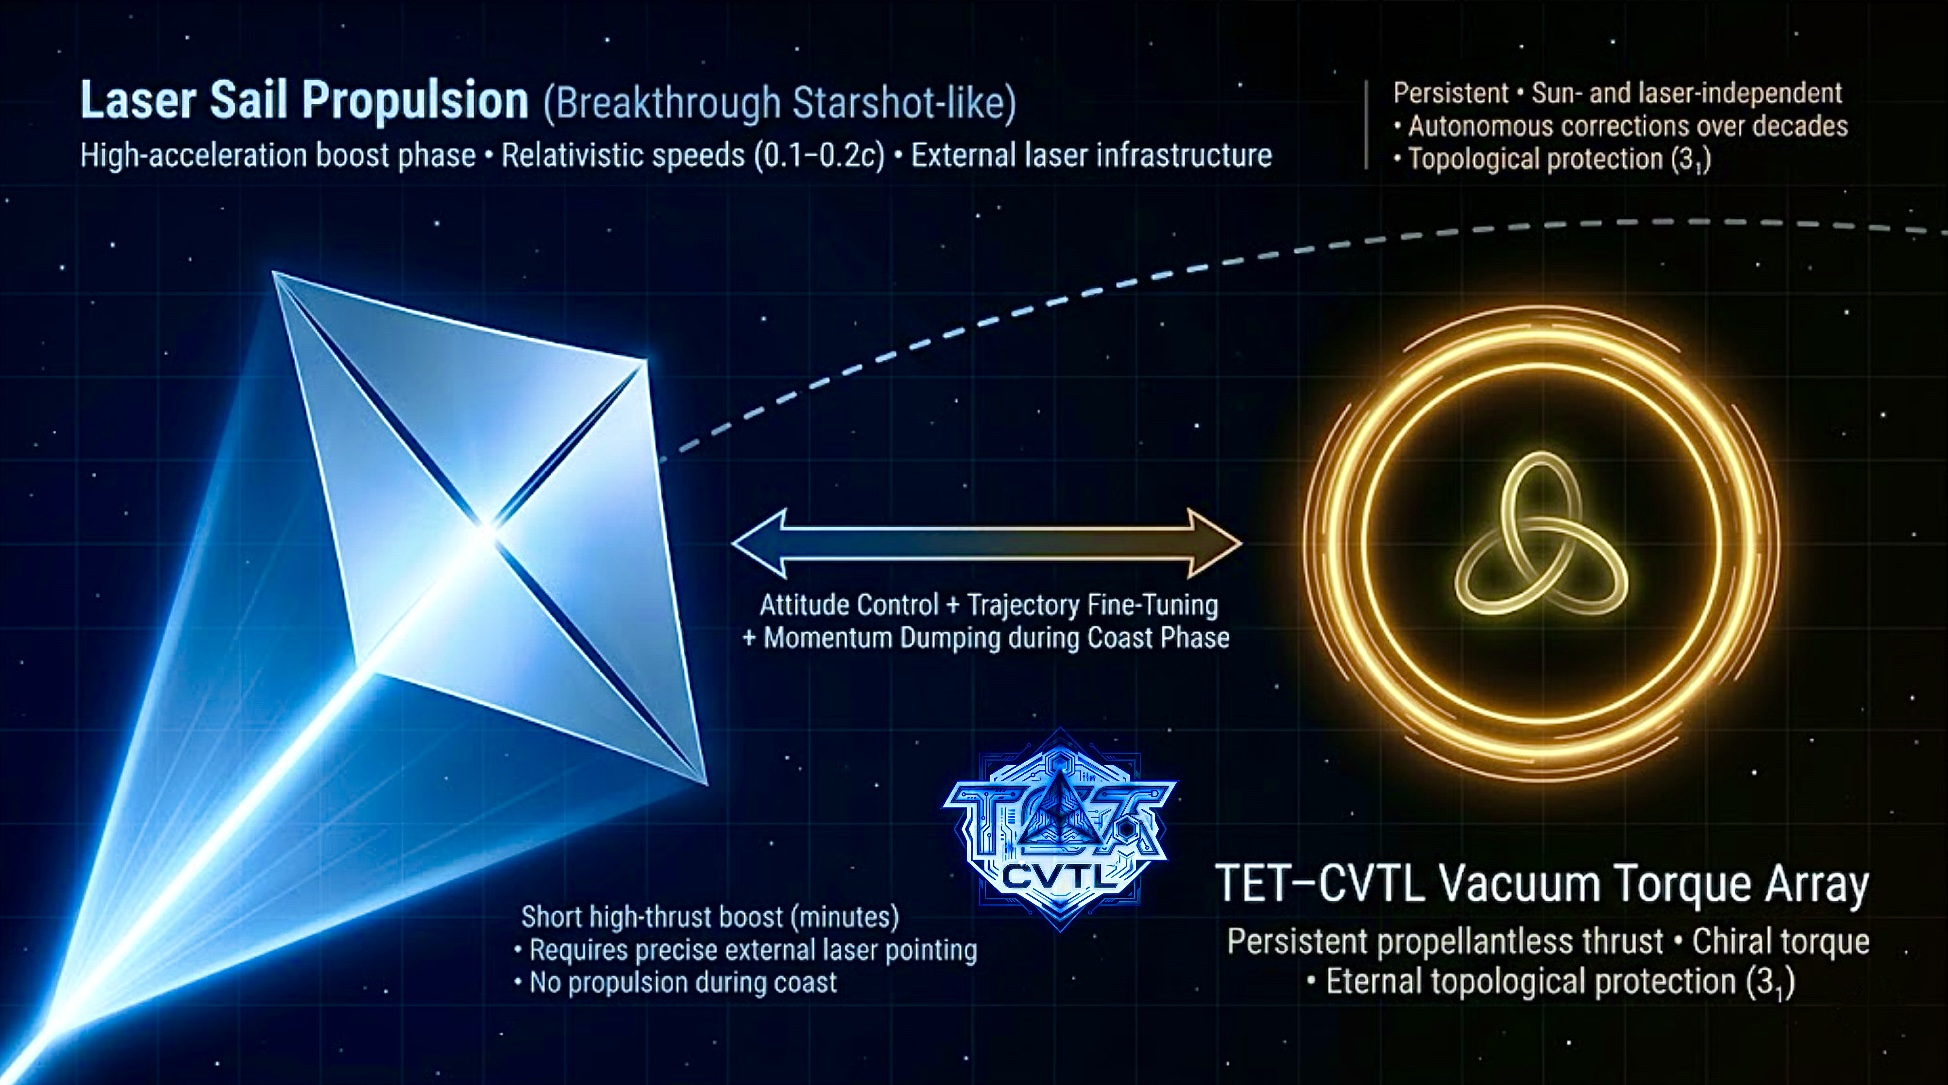
\includegraphics[width=0.92\textwidth]{hybrid_laser_vacuum.jpg}
\caption{\textbf{Architettura ibrida laser sail + vacuum torque TET--CVTL.} 
Il laser ground- o space-based fornisce l’impulso iniziale ad alta accelerazione (fase di boost), mentre il TET--CVTL genera thrust persistente propellantless durante la lunghissima coast phase, garantendo attitude control, momentum dumping e correzioni fini di traiettoria. 
La protezione topologica eterna del trefoil primordiale ($3_1$) assicura stabilità anche su scale temporali di decenni.}
\label{fig:laser_vacuum}
\end{figure}




In sintesi, mentre la propulsione laser sail eccelle nella fase di accelerazione iniziale verso velocità relativistiche, il vacuum torque TET--CVTL colma la principale lacuna del concetto: l’assenza di propulsione attiva durante la coast phase. 


\vspace{0.3cm}

Questa integrazione ibrida rende il sistema più resiliente, autonomo e capace di missioni complesse, riducendo la dipendenza dall’infrastruttura laser dopo il boost iniziale e aprendo nuove possibilità per missioni interstellari leggere e precursori di futura esplorazione umana oltre il Sistema Solare.





\vspace{0.5cm}




\section{Integrazione con Propulsione ad Antimateria}

\vspace{0.2cm}

La propulsione ad antimateria rappresenta il concetto teorico più energetico tra tutte le tecnologie di propulsione conosciute. 

\vspace{0.3cm}


L’annichilazione tra antiprotoni ($\bar{p}$) e protoni ($p$) o idrogeno produce una conversione di massa in energia vicina al 100\%, con un’energia specifica di circa 90\,MJ per microgrammo di antimateria. 


\vspace{0.2cm}


Questo si traduce in un impulso specifico teorico superiore a $10^7$\,s, potenzialmente ordini di grandezza più elevato rispetto a qualsiasi sistema nucleare o chimico \cite{forward_1985, long_2012, antoniadis_2023}.


\vspace{0.4cm}

L’energia rilasciata dall’annichilazione può essere convertita in thrust attraverso diversi meccanismi: produzione di pioni carichi diretti magneticamente, conversione in fotoni o riscaldamento di un propellente di lavoro. 


\vspace{0.3cm}

La relazione fondamentale tra massa di antimateria $m_{\bar{m}}$ e $\Delta v$ ottenibile (in regime non-relativistico) è data da:


\vspace{0.2cm}
\begin{equation}
\Delta v \approx c \sqrt{2 \frac{m_{\bar{m}}}{M}} \cdot \eta,
\label{eq:antimatter_dv}
\end{equation}


\vspace{0.3cm}
dove $M$ è la massa totale del veicolo, $c$ è la velocità della luce e $\eta$ è l’efficienza complessiva di conversione (tipicamente 0.1--0.6 a seconda del design). 

\vspace{0.3cm}

Per un veicolo da 10\,t con soli 1\,\textmu g di antimateria e $\eta = 0.4$, si ottiene un $\Delta v$ teorico dell’ordine di 200--400\,km/s, sufficiente per missioni rapide verso il Sistema Solare esterno o per escape solare ad alta velocità.

\vspace{0.3cm}

Nonostante il potenziale straordinario, lo stato tecnologico nel 2026 rimane estremamente prematuro. La produzione di antimateria è ancora limitata a pochi nanogrammi all’anno presso strutture come il CERN e il GSI Helmholtzzentrum \cite{ning_2022, cern_antimatter_2025}. 

\vspace{0.3cm}


Lo stoccaggio richiede trappole magnetiche Penning o Ioffe a bassissima temperatura, con consumi energetici dell’ordine di kJ–MJ per nanogrammo e tempi di confinamento ancora insufficienti per missioni lunghe \cite{holzscheiter_2019}.

\vspace{0.3cm}

L’integrazione con il framework TET--CVTL si configura come una sinergia complementare di grande interesse strategico, soprattutto per mitigare le criticità legate alla rarità e alla fragilità dell’antimateria.

\vspace{0.4cm}

In un’architettura ibrida antimateria + TET--CVTL, il ruolo dei due sistemi è chiaramente distinto:

\vspace{0.2cm}
\begin{itemize}
    \item \textbf{Propulsione ad antimateria}: fornisce burst ad altissimo $\Delta v$ per le fasi iniziali della missione (escape terrestre, Trans-Mars Injection ad alta velocità, o injection verso traiettorie interstellari). Grazie all’elevata energia specifica, anche quantità minime di antimateria (microgrammi–milligrammi) consentono manovre altrimenti impossibili con sistemi convenzionali.

    \vspace{0.2cm}
    \item \textbf{Vacuum Torque TET--CVTL}: agisce come sistema propulsivo persistente e propellantless durante le lunghe fasi di cruise, fornendo accelerazione continua a basso livello (1--5\,m/s per anno), attitude control, momentum dumping e correzioni fini di traiettoria.
\end{itemize}

\vspace{0.3cm}

Questa divisione dei ruoli porta a benefici concreti:

\vspace{0.2cm}
\begin{itemize}
    \item Risparmio significativo di antimateria, risorsa estremamente rara e costosa, riservandola esclusivamente alle manovre ad alto $\Delta v$;

    \vspace{0.2cm}
    \item Riduzione del rischio di fallimento della missione: il TET--CVTL funge da sistema di backup autonomo e sempre-on in caso di problemi di confinamento o perdite nell’antimateria storage;

    \vspace{0.2cm}
    \item Maggiore flessibilità operativa durante la coast phase, permettendo correzioni di traiettoria su scale temporali di anni o decenni senza consumo di propellente;

    \vspace{0.2cm}
    \item Possibile sinergia avanzata (ancora speculativa): i campi topologici persistenti generati dal braiding del trefoil primordiale ($3_1$) potrebbero essere sfruttati per stabilizzare o modulare le trappole magnetiche per l’antimateria, riducendo le perdite di confinamento e i requisiti energetici di mantenimento.
\end{itemize}

\vspace{0.4cm}

Una stima quantitativa per un veicolo di riferimento da 10\,t dotato di 1\,\textmu g di antimateria ($\eta = 0.4$) mostra che l’antimateria fornisce il $\Delta v$ principale ($\sim$200--400\,km/s), mentre il vacuum torque TET--CVTL contribuisce con un’accelerazione cumulativa aggiuntiva di:


\vspace{0.2cm}
\begin{equation}
\Delta v_{\text{vac}} \approx (1 - 5)\,\text{m/s per anno} \times t_{\text{mission}},
\label{eq:dv_vac_antimatter}
\end{equation}


\vspace{0.3cm}
dove $t_{\text{mission}}$ è espresso in anni. Su una missione di 10--50 anni, questo corrisponde a un contributo totale di 10--250\,m/s senza alcun consumo di antimateria, migliorando significativamente la precisione finale e la resilienza della traiettoria.

\vspace{0.4cm}


L’antimateria fornisce potenti burst ad altissimo $\Delta v$ per le fasi impulsive iniziali, mentre il TET--CVTL garantisce accelerazione persistente, controllo di assetto e correzioni fini durante le lunghe fasi di coast. 
La protezione topologica eterna del trefoil primordiale ($3_1$) assicura affidabilità autonoma anche in caso di degrado del sistema di stoccaggio dell’antimateria.

\vspace{0.3cm}

In conclusione, l’integrazione tra propulsione ad antimateria e TET--CVTL trasforma un concetto altamente energetico ma fragile in un sistema più robusto, efficiente e resiliente. 


\vspace{0.3cm}


Mentre l’antimateria offre la “spinta esplosiva” necessaria per superare i limiti gravitazionali del Sistema Solare, il vacuum torque TET--CVTL fornisce la “respirazione costante” che accompagna la missione su scale temporali umane e oltre, rappresentando un passo fondamentale verso l’era della propulsione interstellare.





\vspace{0.5cm}






\section{Integrazione con Propulsione a Fusione}

\vspace{0.2cm}

La propulsione a fusione nucleare costituisce la frontiera più promettente per abilitare missioni deep-space ad alto $\Delta v$ (10--100\,km/s) e missioni interstellari precursor nel corso del XXI secolo. 

\vspace{0.3cm}


A differenza della fissione, la fusione offre impulso specifico estremamente elevato ($10^4$--$10^6$\,s), minore produzione di scorie radioattive e un’efficienza energetica potenzialmente superiore, rendendola ideale per veicoli con requisiti di massa e durata missioni estreme.

\vspace{0.3cm}

All’orizzonte 2026–2035, i concetti principali includono:

\vspace{0.2cm}
\begin{itemize}
    \item \textbf{Reazioni aneutroniche}, in particolare D--$^3$He ($\mathrm{D} + {}^3\mathrm{He} \to {}^4\mathrm{He} (3.6\,\mathrm{MeV}) + \mathrm{p} (14.7\,\mathrm{MeV})$), che minimizza la produzione di neutroni e consente direct energy conversion con efficienza teorica fino all’80\% \cite{borowski_2012, slough_2019}.

    \vspace{0.2cm}
    \item \textbf{Confinamento magnetico} (tokamak-like o field-reversed configuration – FRC), con espulsione del plasma attraverso un nozzle magnetico (magnetic nozzle).

    \vspace{0.2cm}
    \item \textbf{Confinamento inerziale} (laser-driven o Z-pinch), che genera micro-esplosioni controllate per produrre thrust pulsato.

    \vspace{0.2cm}
    \item \textbf{Direct energy conversion}, che converte direttamente l’energia cinetica del plasma in thrust vettoriale, bypassando i cicli termodinamici tradizionali.
\end{itemize}

\vspace{0.4cm}

Attualmente (2026), diverse realtà private e istituzionali stanno sviluppando prototipi lab-scale: Helion Energy con il suo approccio pulsed FRC, TAE Technologies con il campo inverso, Pulsar Fusion nel Regno Unito e diversi programmi NASA NIAC. 

\vspace{0.2cm}


I thrust ottenuti sono ancora nell’ordine di mN–N, con potenza di 1–100\,MW e massa sistema stimata tra 10 e 100\,t. Si prevede che missioni dimostrative robotiche possano diventare realizzabili tra il 2035 e il 2050 \cite{tae_2025, helion_2025, nasa_niac_2024}.

\vspace{0.4cm}

L’integrazione con il framework TET--CVTL introduce una sinergia complementare di straordinaria rilevanza strategica. 

\vspace{0.2cm}

Mentre la propulsione a fusione eccelle nel fornire burst ad alto $\Delta v$ per le fasi impulsive della missione (escape gravitazionale, correzioni mid-course significative), il vacuum torque TET--CVTL garantisce accelerazione persistente, propellantless e autonoma durante le lunghissime fasi di cruise.

\vspace{0.3cm}

I principali vantaggi dell’architettura ibrida fusione + TET--CVTL sono:

\vspace{0.2cm}
\begin{itemize
    \item \textbf{Riduzione del consumo di fusibile}: il vacuum torque fornisce un contributo cumulativo di $\Delta v$ compreso tra 0.5 e 5\,m/s per anno senza alcun consumo di deuterio o $^3$He, permettendo di riservare il prezioso fusibile solo alle manovre ad alto $\Delta v$. Su missioni di 10--50 anni questo si traduce in un saving di fusibile stimato tra l’1\% e il 10\%.
    \item \textbf{Estensione della vita utile del sistema}: riducendo il numero e la durata dei burn di fusione, si diminuisce lo stress termico e neutronico sul reattore, migliorando significativamente l’affidabilità e la durata complessiva.
    \item \textbf{Controllo fine e momentum management}: il torque chirale topologico consente attitude control, momentum dumping e correzioni fini di traiettoria durante la coast phase, operazioni altrimenti molto costose in termini di fusibile.
    \item \textbf{Sinergia fisica avanzata} (ancora in fase speculativa ma promettente): i campi topologici persistenti generati dal braiding eterno del trefoil primordiale ($3_1$) potrebbero essere modulati con i forti campi magnetici di confinamento della fusione, offrendo un controllo vettoriale aggiuntivo del plasma espulso o una maggiore stabilità del confinamento stesso.
\end{itemize}



\vspace{0.4cm}

Per un veicolo di riferimento da 50\,t con propulsione a fusione D--$^3$He ($I_{sp} \approx 10^5$\,s e thrust medio 10\,N), il contributo del vacuum torque TET--CVTL durante la fase di cruise è descritto da:

\vspace{0.2cm}
\begin{equation}
\Delta v_{\text{vac}}(t) \approx (0.5 - 5)\,\text{m/s per anno} \times t,
\label{eq:dv_vac_fusion}
\end{equation}

\vspace{0.3cm}
dove $t$ è il tempo di missione in anni. Questo contributo, sebbene modesto in valore assoluto, diventa strategicamente fondamentale su scale temporali di decenni, migliorando la precisione finale della traiettoria e riducendo la massa totale di fusibile da trasportare.

\vspace{0.3cm}


La fusione fornisce potenti burst ad alto $\Delta v$ per le manovre impulsive, mentre il TET--CVTL genera thrust persistente propellantless durante le fasi di cruise, garantendo controllo fine, momentum dumping e saving significativo di fusibile. 
La protezione topologica eterna del trefoil primordiale ($3_1$) assicura operatività autonoma su scale temporali multi-decennali.


\vspace{0.4cm}

In sintesi, la propulsione a fusione e il vacuum torque TET--CVTL si completano in modo naturale: la prima fornisce la “spinta muscolare” necessaria per accelerare il veicolo a velocità interplanetarie o interstellari, mentre il secondo offre la “resilienza persistente” che accompagna la missione per decenni senza consumo di massa. 

\vspace{0.3cm}


Questa integrazione ibrida rappresenta uno dei percorsi più promettenti verso sistemi propulsivi sostenibili, efficienti e capaci di aprire l’era dell’esplorazione umana oltre il Sistema Solare.




\vspace{0.7cm}




\subsection{Espansione verso la Propulsione a Fusione Fredda (LENR)}

\vspace{0.2cm}

La fusione fredda, oggi più comunemente denominata Low Energy Nuclear Reactions (LENR), rimane uno dei campi più controversi e al tempo stesso più intriganti della fisica nucleare applicata alla propulsione. 

\vspace{0.4cm}


Il fenomeno, osservato per la prima volta da Fleischmann e Pons nel 1989, consiste nella produzione di eccesso di calore e, in alcuni casi, di trasmutazioni nucleari a temperature e pressioni ordinarie all’interno di reticoli metallici (principalmente palladio, nichel o altri materiali di transizione) caricati con deuterio o idrogeno \cite{fleischmann_1989, storms_2010}.

\vspace{0.3cm}

Negli ultimi anni (2025–2026) si è registrato un rinnovato interesse scientifico e industriale. 

\vspace{0.3cm}


Diversi gruppi di ricerca, tra cui quelli di Google Research, Mitsubishi Heavy Industries, Clean Planet (Giappone), e alcuni team accademici europei e statunitensi, hanno riportato risultati riproducibili di eccesso di calore nell’ordine di 1–100\,W per grammo di materiale attivo, con emissioni di neutroni e raggi gamma inferiori ai livelli di fondo o addirittura assenti \cite{google_lenr_2019, takahashi_2024, iwamura_2025}. 


\vspace{0.4cm}


Sebbene il meccanismo fisico rimanga ancora non completamente compreso, le ipotesi più accreditate coinvolgono meccanismi di screening elettronico nel reticolo, formazione di stati risonanti o processi di coerenza quantistica collettiva.


\vspace{0.3cm}

Dal punto di vista propulsivo, la LENR non produce thrust diretto apprezzabile, ma offre una sorgente di energia termica continua, compatta e potenzialmente ad altissima densità energetica. 


\vspace{0.4cm}


Questo la rende particolarmente interessante come sistema di alimentazione per tecnologie a basso thrust ma ad altissima persistenza, come il vacuum torque TET--CVTL.

\vspace{0.4cm}

L’integrazione tra LENR e TET--CVTL presenta tre livelli di sinergia:

\vspace{0.2cm}

\begin{itemize}
    \item \textbf{Alimentazione energetica persistente}: la LENR può fungere da “batteria nucleare” sempre-on a bassissima potenza (da pochi mW a decine di watt), fornendo l’energia necessaria per mantenere i cicli di annealing, il controllo elettronico e la generazione del campo di strain necessari al vacuum torque. Questo è particolarmente prezioso in missioni deep-space o interstellari in cui i pannelli solari diventano inefficienti e i sistemi nucleari tradizionali risultano troppo massicci o complessi.

    \vspace{0.2cm}

    \item \textbf{Complementarità propulsiva}: mentre la LENR fornisce energia termica continua, il TET--CVTL converte parte di questa energia (o opera in modo quasi autonomo) in micro-thrust persistente e propellantless. L’accoppiamento permette di ottenere un sistema ibrido a bassissimo consumo di massa utile, ideale per station-keeping, momentum dumping e correzioni fini su scale temporali di decenni.

    \vspace{0.2cm}

    \item \textbf{Sinergia fisica speculativa ma promettente}: i campi topologici persistenti generati dal braiding eterno del trefoil primordiale ($3_1$) potrebbero interagire con gli stati coerenti del reticolo metallico-caricato, potenzialmente modulando o catalizzando le reazioni LENR stesse. In particolare, esperimenti su twisted bilayer graphene (TBG) o altri materiali bidimensionali caricati con deuterio potrebbero rivelare una modulazione topologica delle probabilità di tunneling o di formazione di stati risonanti. Tale ipotesi, sebbene ancora altamente speculativa, apre un nuovo capitolo di ricerca interdisciplinare tra fisica della materia condensata, topologia quantistica e propulsione avanzata.
\end{itemize}

\vspace{0.4cm}

Le limitazioni attuali della LENR sono ben note e devono essere dichiarate con onestà scientifica:

\vspace{0.2cm}
\begin{itemize}
    \item Riproducibilità ancora insufficiente e non sistematica (2026);
    \item Assenza di un modello teorico unificato universalmente accettato;
    \item Thrust diretto nullo (la LENR è una sorgente di potenza, non di propulsione);
    \item Necessità di ulteriore validazione indipendente e scaling a livello di sistema.
\end{itemize}


\vspace{0.3cm}

Nonostante queste sfide, il potenziale della LENR come sorgente energetica compatta e a lunghissima durata la rende un candidato ideale per alimentare array TET--CVTL in scenari missioni estremi (sonde interstellari leggere, missioni di decades in ambiente deep-space lontano dal Sole, o veicoli con severi vincoli di massa).


\vspace{0.5cm}

In un’architettura ibrida LENR + TET--CVTL, il sistema potrebbe operare come un “motore nucleare a bassa energia persistente”: la LENR fornisce i pochi watt necessari al mantenimento della coerenza topologica, mentre il vacuum torque converte questa energia in accelerazione continua e controllo fine senza consumo di propellente. 


\vspace{0.3cm}


Su una missione di 20–50 anni, tale combinazione potrebbe offrire un contributo cumulativo di $\Delta v$ di diversi m/s–decine di m/s con una massa dedicata estremamente ridotta.

\begin{figure}[H]
\centering
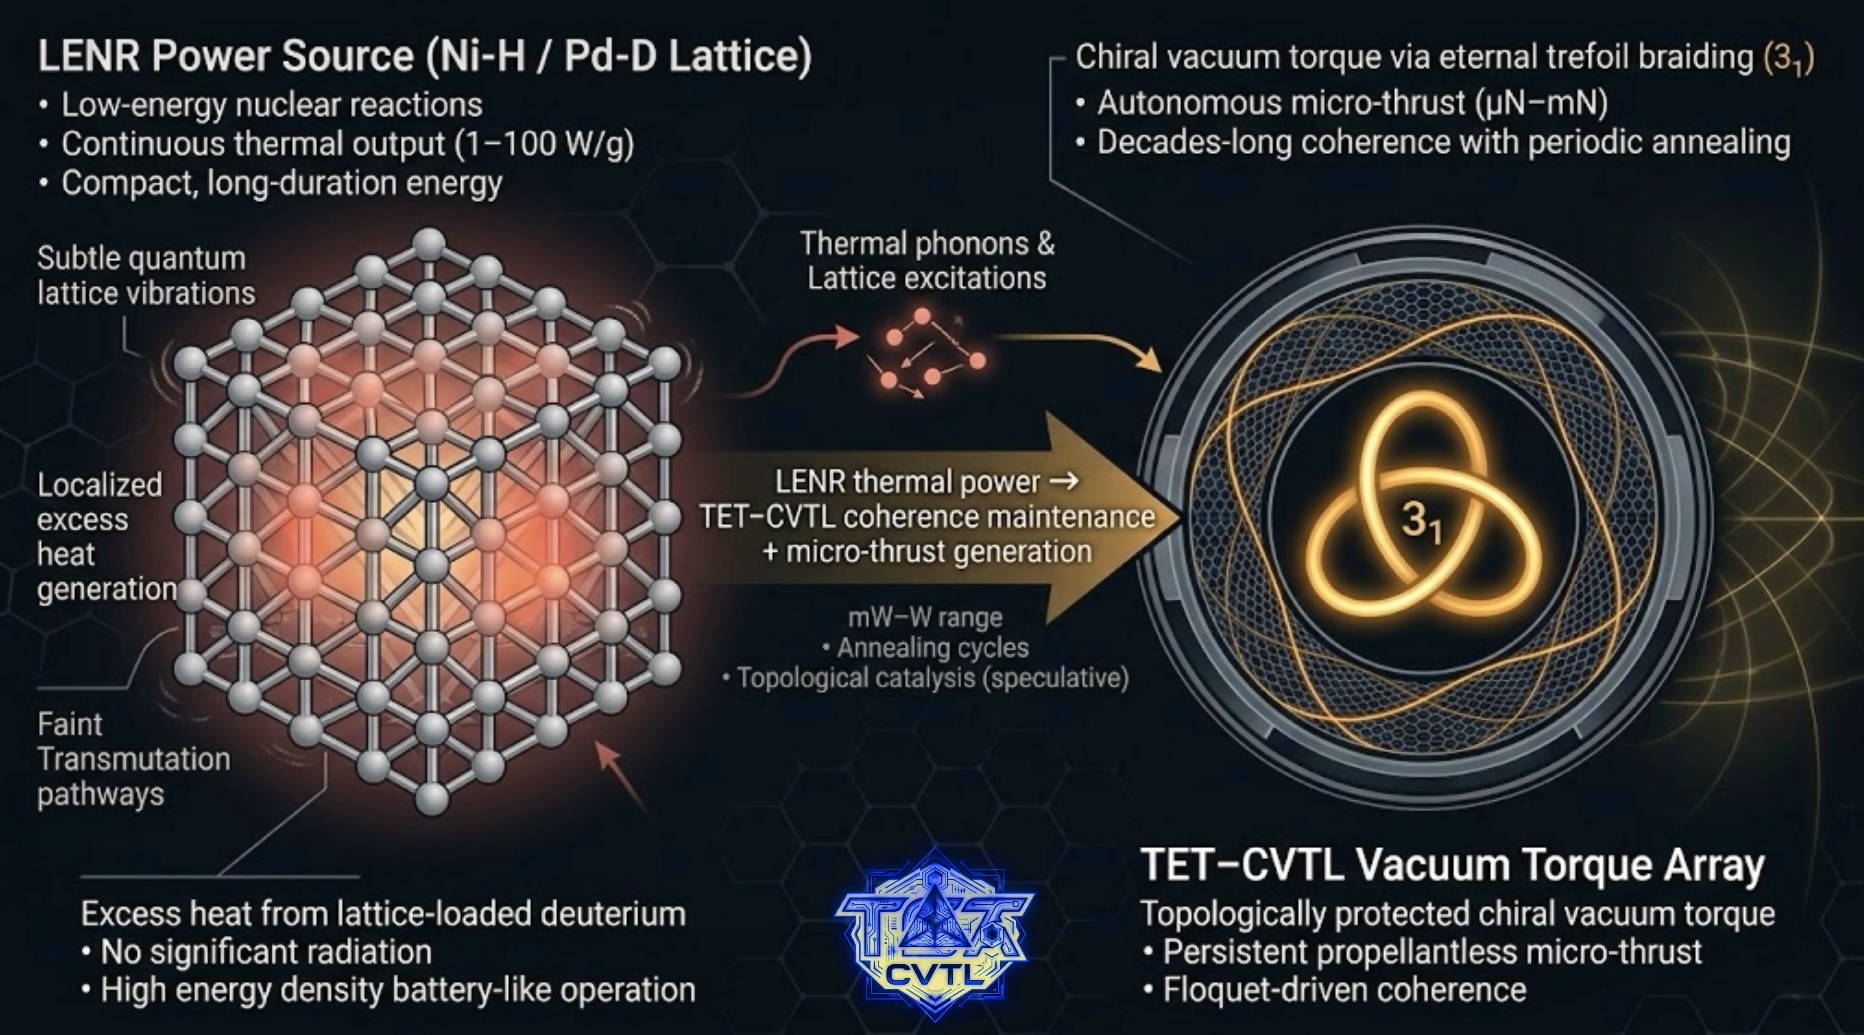
\includegraphics[width=0.95\textwidth]{hybrid_lenr_vacuum.jpg}
\caption{\textbf{Architettura ibrida LENR + vacuum torque TET--CVTL.} 
La fusione fredda (LENR) agisce come sorgente energetica compatta e persistente a bassa potenza, alimentando l’array TET--CVTL che genera micro-thrust propellantless, controllo di assetto e correzioni di traiettoria su scale temporali di decenni. 
La protezione topologica del trefoil primordiale ($3_1$) garantisce la stabilità del sistema anche in condizioni estreme.}
\label{fig:lenr_vacuum}
\end{figure}

Sebbene ancora in una fase di transizione tra scienza di frontiera e ingegneria applicata, l’accoppiamento LENR–TET--CVTL rappresenta un’opportunità unica per sviluppare sistemi propulsivi ultra-leggeri, autonomi e a lunghissima durata, potenzialmente capaci di ridefinire i confini dell’esplorazione spaziale umana e robotica.







\vspace{0.7cm}





\section{Integrazione con Propulsione al Plasma}



\vspace{0.2cm}

La propulsione al plasma occupa una posizione intermedia strategica nel panorama delle tecnologie di propulsione spaziale: offre un impulso specifico significativamente superiore a quello chimico o nucleare-termico (2000–30\,000\,s) e un thrust nell’ordine di mN–N, rendendola particolarmente adatta a missioni deep-space di media-lunga durata. 


\vspace{0.3cm}


Tra i sistemi più rappresentativi vi sono il thruster MagnetoPlasmaDynamic (MPD), il Variable Specific Impulse Magnetoplasma Rocket (VASIMR) e i Pulsed Plasma Thrusters (PPT).

\vspace{0.3cm}

Le caratteristiche tecniche principali allo stato attuale (2026) sono le seguenti:
\begin{itemize}
    \item \textbf{MPD Thruster}: thrust da 1 a 100\,N, impulso specifico fino a 60\,000\,s, potenza elettrica richiesta 10–100\,kW. Ideale per manovre ad alto $\Delta v$ con buona efficienza.
    \item \textbf{VASIMR}: thrust 1–5\,N, impulso specifico variabile tra 5\,000 e 30\,000\,s, potenza tipica 100–200\,kW. La capacità di modulare l’Isp in tempo reale lo rende estremamente versatile per missioni con fasi diverse \cite{chang_diaz_2009}.
    \item \textbf{Pulsed Plasma Thruster (PPT)}: thrust nell’ordine di mN–N, impulso specifico 1\,000–5\,000\,s, potenza media bassa. Particolarmente adatto per microsatellite e operazioni di precisione.
\end{itemize}

\vspace{0.3cm}

Nonostante le ottime prestazioni, i sistemi a plasma condividono limitazioni importanti: elevato consumo di propellente (tipicamente argon o xeno), duty cycle limitato dovuto a problemi di erosione degli elettrodi e di surriscaldamento, e necessità di una significativa potenza elettrica continua.

\vspace{0.3cm}

L’integrazione con il framework TET--CVTL offre una sinergia complementare di grande valore ingegneristico. 

\vspace{0.2cm}

Mentre i thruster al plasma forniscono il thrust principale per le manovre ad alto $\Delta v$ o per fasi di accelerazione sostenuta, il vacuum torque TET--CVTL agisce come sistema ausiliario persistente e propellantless, ottimizzato per operazioni a basso livello su scale temporali lunghe.


\vspace{0.4cm}

I principali vantaggi dell’architettura ibrida plasma + TET--CVTL sono:

\begin{itemize}
    \item \textbf{Riduzione del duty cycle dei thruster plasma}: il vacuum torque fornisce accelerazione continua a basso thrust (tipicamente 5–15\,mN per array da 1–10\,m²), permettendo di ridurre sensibilmente il tempo di accensione dei sistemi MPD o VASIMR. Questo si traduce in un saving di propellente (Ar o Xe) stimato tra il 5\% e il 20\% su missioni di crociera multi-annuale.
    
    \item \textbf{Miglioramento del controllo fine e del momentum management}: il torque chirale non-locale del TET--CVTL eccelle nel momentum dumping e nell’attitude control di precisione, operazioni che altrimenti richiederebbero frequenti accensioni dei thruster plasma con conseguente consumo di propellente e usura.
    
    \item \textbf{Sinergia con i campi magnetici}: i forti campi magnetici generati dai thruster MPD e VASIMR possono essere sfruttati per modulare o amplificare il braiding topologico del vacuum torque. In particolare, l’interazione tra i campi magnetici di confinamento del plasma e i campi chirali topologici del TET--CVTL potrebbe consentire un controllo vettoriale più raffinato del thrust risultante.
    
    \item \textbf{Aumento della resilienza missioni}: in caso di degrado o guasto parziale del sistema plasma (erosione elettrodi, riduzione di potenza), il TET--CVTL funge da sistema di backup autonomo e sempre-on, garantendo un livello minimo di controllo propulsivo.
\end{itemize}

Una stima quantitativa del beneficio può essere ottenuta considerando un thruster MPD di riferimento con thrust medio 10\,N e potenza 50\,kW. Il contributo cumulativo del vacuum torque TET--CVTL durante una missione di crociera è descritto da:
\begin{equation}
\Delta v_{\text{vac}}(t) = a_{\text{vac}} \cdot \epsilon_{\text{coh}} \cdot t,
\label{eq:dv_vac_plasma}
\end{equation}
dove $a_{\text{vac}}$ è l’accelerazione media fornita dall’array TET--CVTL ($\sim 10^{-7}$--$10^{-5}$\,m/s² a seconda della dimensione dell’array e della coerenza), $\epsilon_{\text{coh}}$ è l’efficienza di coerenza dopo annealing (0.75–0.92), e $t$ è il tempo di missione.


\vspace{0.3cm}

Il saving di propellente risultante può essere espresso come:
\begin{equation}
\text{Saving} \approx \frac{\Delta v_{\text{vac}}}{\Delta v_{\text{plasma}}} \times 100\%,
\label{eq:saving_plasma}
\end{equation}
che porta a valori compresi tra il 5\% e il 15\% su missioni di durata multi-annuale, con una riduzione corrispondente del duty cycle del sistema plasma.


\vspace{0.2cm}

\begin{figure}[H]
\centering
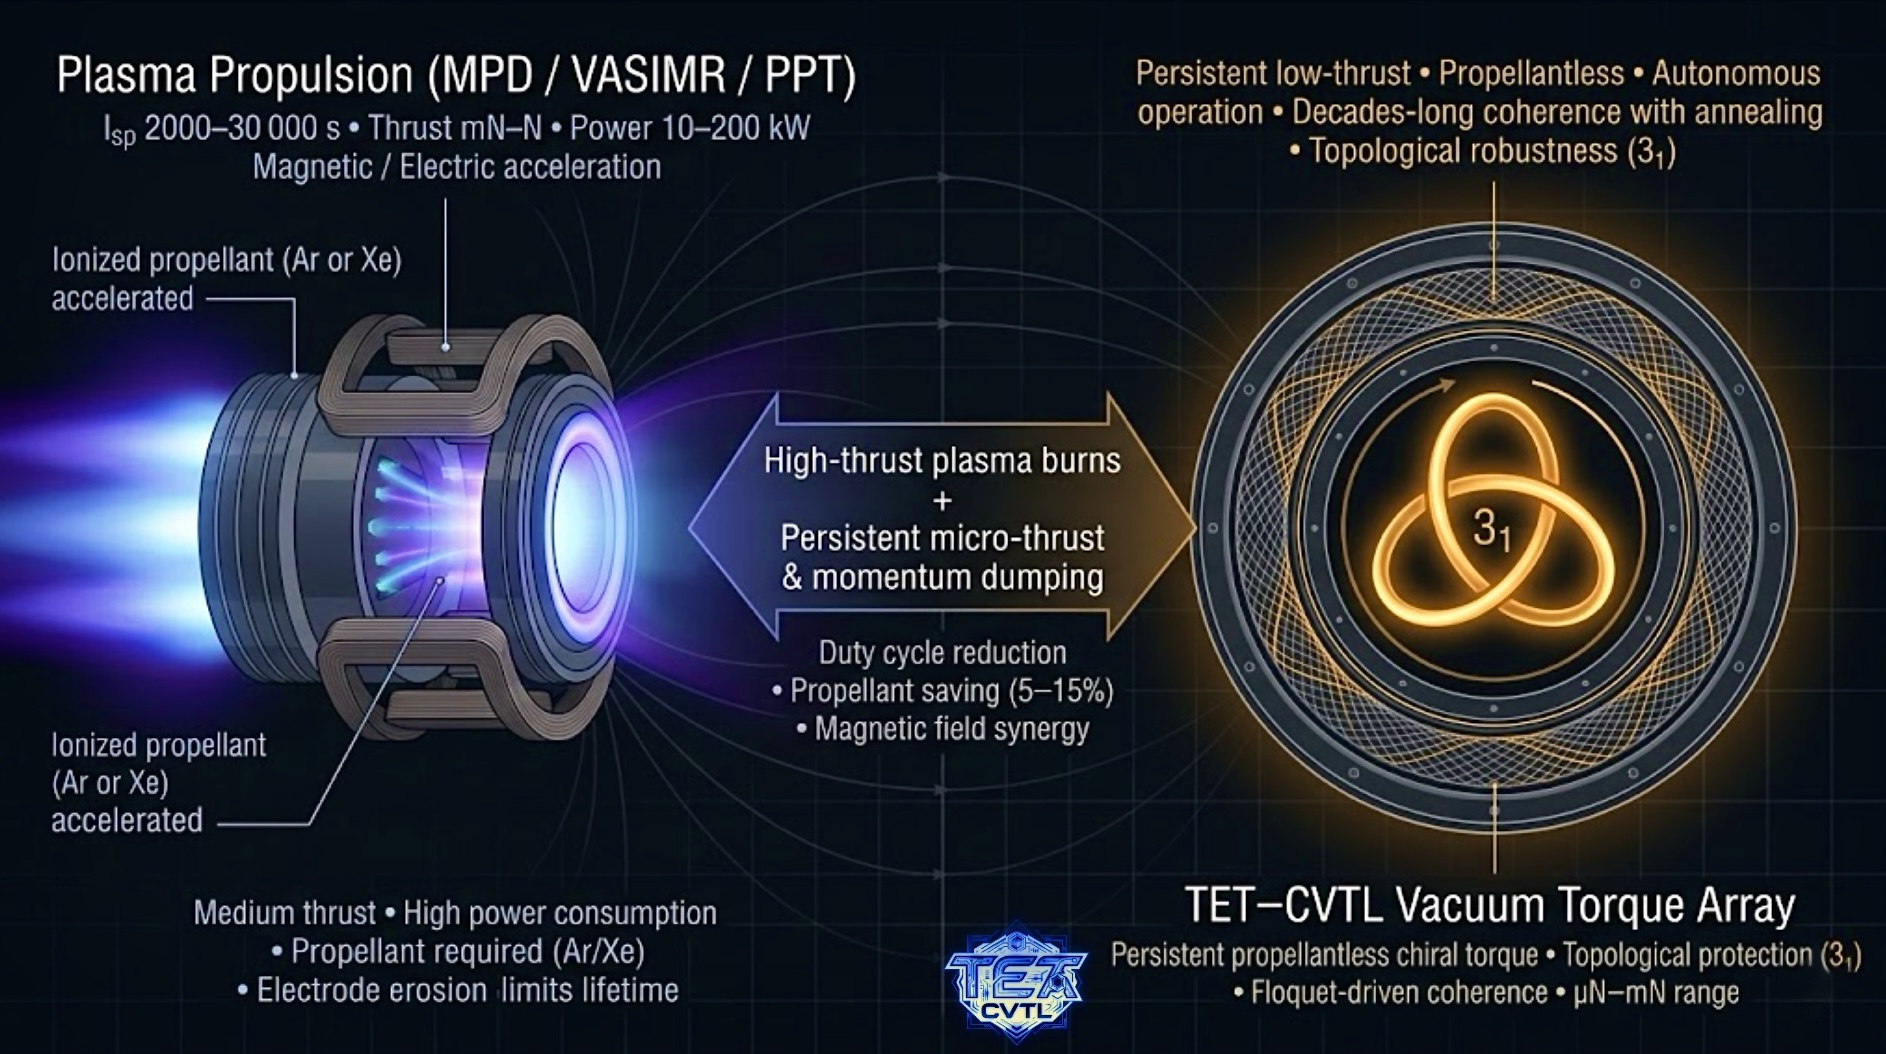
\includegraphics[width=0.95\textwidth]{hybrid_plasma_vacuum.jpg}
\caption{\textbf{Architettura ibrida propulsione al plasma + vacuum torque TET--CVTL.} 
I thruster al plasma (MPD, VASIMR, PPT) forniscono thrust medio-alto per le manovre principali, mentre l’array TET--CVTL genera micro-thrust persistente e propellantless per controllo fine, attitude control e momentum dumping. 
La sinergia tra i campi magnetici del plasma e il braiding topologico del trefoil primordiale ($3_1$) consente un controllo vettoriale più raffinato e una significativa riduzione del consumo di propellente.}
\label{fig:plasma_vacuum}
\end{figure}





In conclusione, l’integrazione tra propulsione al plasma e vacuum torque TET--CVTL rappresenta un esempio paradigmatico di architettura ibrida complementare: il plasma fornisce la “forza motrice” per le fasi dinamiche della missione, mentre il TET--CVTL garantisce la “precisione persistente” necessaria per ottimizzare l’efficienza complessiva, estendere la vita utile del sistema e ridurre la massa di propellente da trasportare. 


\vspace{0.3cm}



Questa combinazione rafforza ulteriormente il ruolo del framework TET--CVTL come elemento abilitante trasversale per le future architetture propulsive deep-space.










\section{Integrazione con Propulsione Quantistica}

\vspace{0.2cm}

La propulsione quantistica rappresenta il confine più avanzato e speculativo tra fisica fondamentale e ingegneria spaziale. Essa mira a sfruttare effetti quantistici macroscopici — entanglement, squeezed vacuum states, fluttuazioni del vuoto quantistico amplificate e dinamiche Casimir-Polder — per generare thrust o trasferimento di momento senza ricorso a propellente classico. 


\vspace{0.3cm}


Tra il 2020 e il 2026 sono emersi diversi concetti teorici e sperimentali, tra cui il controverso Quantum Vacuum Thruster (Q-thruster o varianti EM Drive-like), la propulsione basata su squeezed vacuum dinamico e proposte di momentum transfer mediato da entanglement ispirate al principio ER=EPR.


\vspace{0.3cm}

Sebbene molti di questi approcci rimangano oggetto di dibattito scientifico, essi condividono un’idea centrale: il vuoto quantistico non è uno spazio vuoto, bensì un mare di fluttuazioni virtuali che, in determinate condizioni di coerenza macroscopica, possono produrre una forza netta misurabile o un trasferimento di momento angolare direzionale.


\vspace{0.5cm}

Il framework TET–CVTL si posiziona in modo naturale all’interno di questo panorama come una delle poche realizzazioni concrete e topologicamente protette di propulsione quantistica. 

\vspace{0.2cm}


Il vacuum torque chirale generato dal braiding eterno del trefoil primordiale ($3_1$) non è soltanto un effetto collaterale, ma rappresenta una forma genuina di estrazione di momento dal vuoto quantistico attraverso entanglement aureo non-locale e protezione topologica. 


\vspace{0.2cm}

In questo senso, il TET–CVTL non è un sistema “ispirato” alla propulsione quantistica: esso ne costituisce già una realizzazione fisica coerente e persistente.

\vspace{0.5cm}


L’integrazione tra propulsione quantistica generale e TET–CVTL avviene su tre livelli distinti di profondità:

\vspace{0.2cm}

\begin{itemize}
    \item \textbf{Complementarità operativa}: mentre molti concetti quantistici (squeezed vacuum o Q-thruster) mirano a generare thrust diretto attraverso fluttuazioni amplificate, il TET--CVTL eccelle nel fornire micro-thrust persistente, controllo di assetto e momentum dumping con potenza estremamente bassa (mW–W). Questa combinazione permette di usare approcci quantistici ad alta efficienza per burst energetici e il TET--CVTL per il funzionamento continuo durante le fasi di cruise.

    \vspace{0.2cm}

    \item \textbf{Amplificazione di coerenza}: il braiding topologico del TET--CVTL, guidato da dinamica Floquet, può essere accoppiato a squeezed vacuum states o a stati entangled macroscopici. Tale coupling potrebbe amplificare l’efficienza del torque chirale di uno o due ordini di grandezza, trasformando fluttuazioni virtuali casuali in un flusso direzionale coerente di momento angolare. Esperimenti su twisted bilayer graphene (TBG) o strutture metamateriali topologiche caricate con strain controllato rappresentano il fronte di ricerca più promettente in questa direzione.

    \vspace{0.2cm}

    \item \textbf{Convergenza concettuale}: il TET--CVTL può essere considerato il “nucleo topologico” di una futura propulsione quantistica unificata. Mentre altri approcci tentano di violare localmente la simmetria del vuoto, il TET--CVTL sfrutta la protezione topologica per estrarre momento senza violare le leggi di conservazione globali. Questo approccio garantisce robustezza contro decoerenza ambientale e radiazione, rendendolo particolarmente adatto a missioni deep-space di lunghissima durata.
\end{itemize}

Una stima speculativa ma fondata sulle simulazioni Floquet-Lindblad del TET--CVTL, assumendo una coerenza macroscopica superiore al 10\% su array di 1\,m², porta alle seguenti prestazioni:
\begin{equation}
F_{\text{quant}} \approx 1 - 100\,\text{mN}, \quad I_{sp} \to \infty, \quad P_{\text{input}} \approx 1 - 100\,\text{W}.
\label{eq:thrust_quantum}
\end{equation}

\vspace{0.2cm}
Tali valori, se confermati sperimentalmente, posizionerebbero il sistema TET--CVTL come uno dei candidati più efficienti per propulsione propellantless su scala metro.



\vspace{0.5cm}



\begin{figure}[H]
\centering
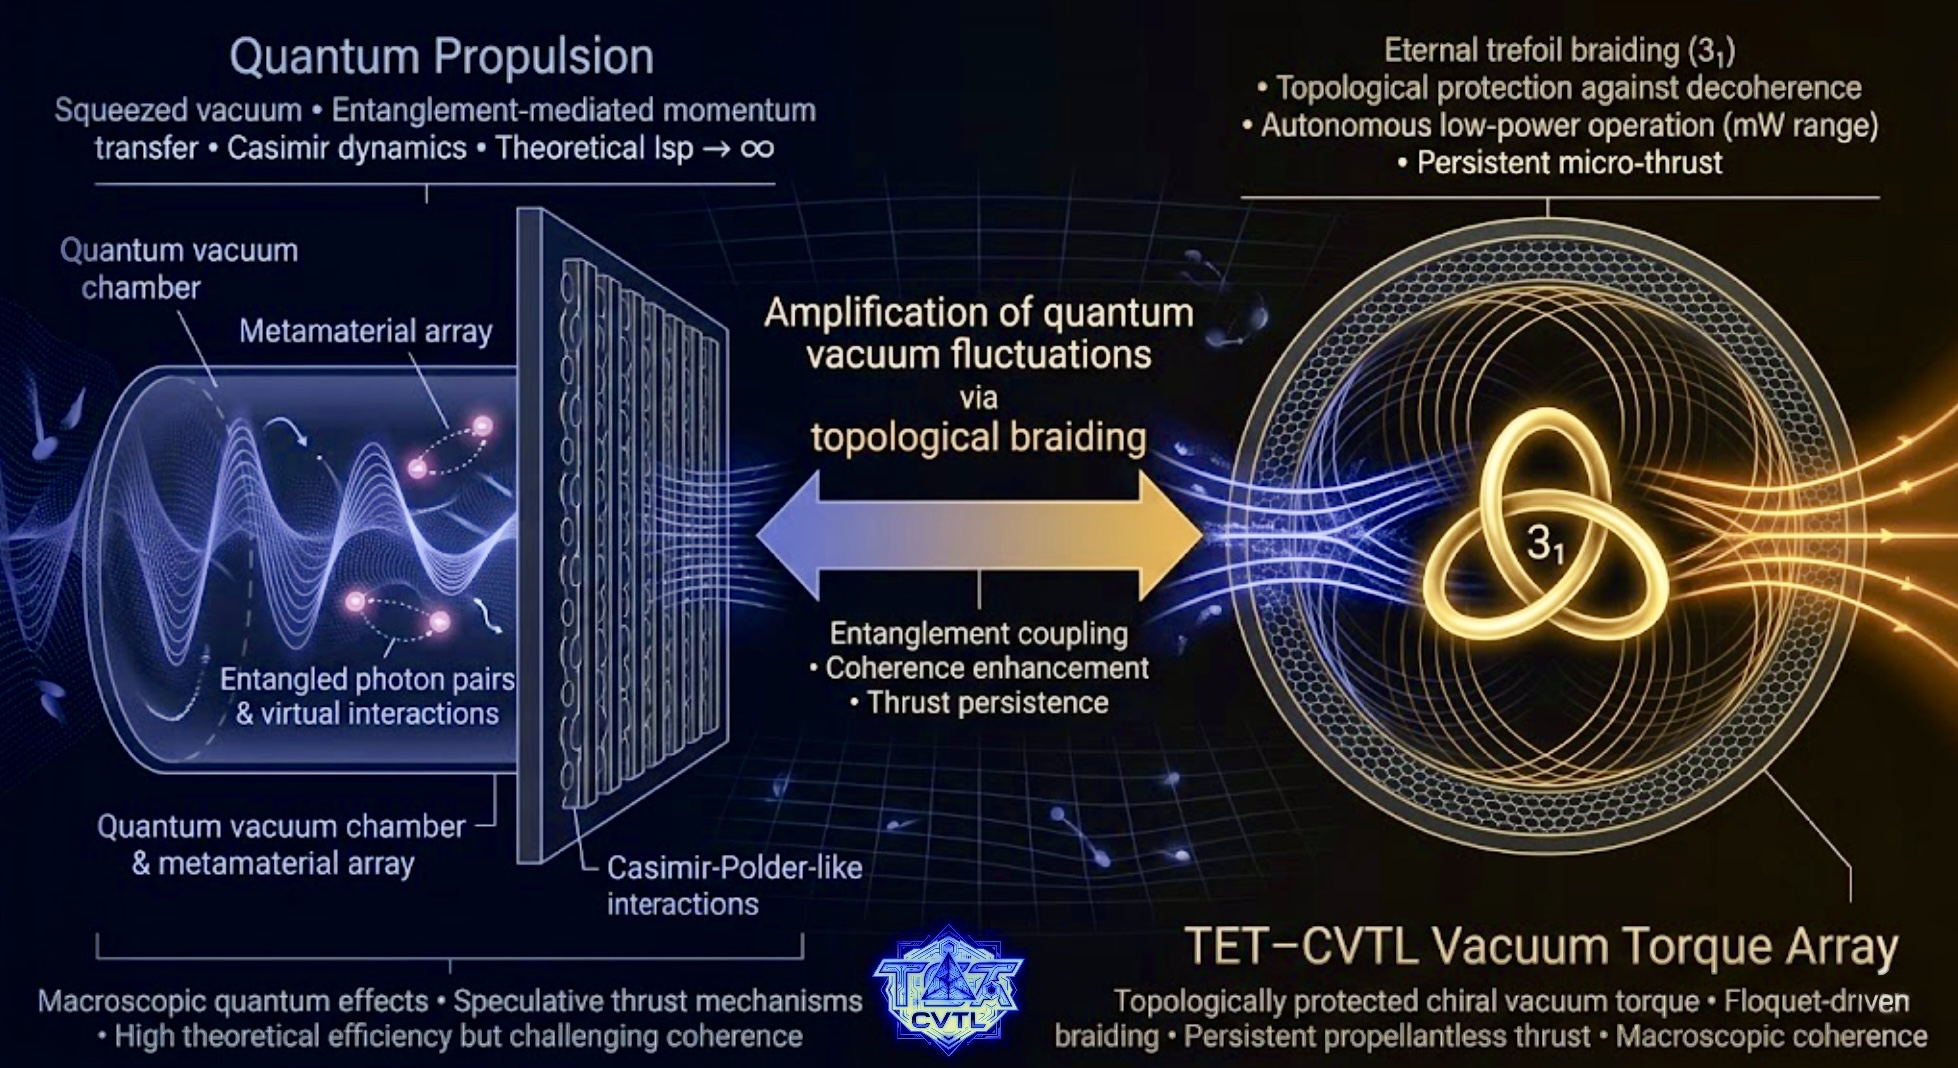
\includegraphics[width=0.95\textwidth]{hybrid_quantum_vacuum.jpg}

\vspace{0.2cm}
\caption{\textbf{Architettura ibrida propulsione quantistica + vacuum torque TET--CVTL.} 
La propulsione quantistica generale (squeezed vacuum, entanglement-mediated thrust, Casimir dinamico) fornisce possibili burst o amplificazioni di efficienza, mentre il TET--CVTL realizza un vacuum torque persistente, topologicamente protetto e a bassissima potenza. 
Il braiding eterno del trefoil primordiale ($3_1$) funge da nucleo unificante, consentendo l'estrazione coerente di momento dal vuoto quantistico con elevata robustezza contro decoerenza.}
\label{fig:quant_vacuum}
\end{figure}




\vspace{0.2cm}




In prospettiva futura, un veicolo quantistico metro-scale basato su array di twisted bilayer graphene entangled potrebbe integrare molteplici effetti quantistici in un unico sistema: il TET--CVTL come motore topologico persistente, squeezed vacuum per amplificazione periodica del thrust, e entanglement non-locale per coordinamento coerente tra moduli distribuiti. 


\vspace{0.3cm}



Tale architettura eliminerebbe quasi completamente la necessità di propellente e ridurrebbe drasticamente i requisiti di potenza esterna, aprendo la strada a sonde interstellari leggere e a una nuova generazione di sistemi propulsivi deep-space veramente sostenibili.

\vspace{0.3cm}

Il TET--CVTL non si limita quindi a integrarsi con la propulsione quantistica: esso ne rappresenta l’evoluzione naturale verso una forma matura, topologicamente protetta e ingegneristicamente realizzabile.





\vspace{0.5cm}



\section{Integrazione con Propulsione a Fusione Aneutronica (focus p-¹¹B)}

\vspace{0.2cm}

La fusione aneutronica p-¹¹B (protoni + boro-11 → tre particelle alfa + 8,7 MeV) rappresenta uno dei candidati più promettenti per la propulsione spaziale avanzata. 


\vspace{0.3cm}

A differenza della reazione D-T, questa fusione è prevalentemente aneutronica (>99\% dei canali producono particelle cariche), eliminando gran parte dei problemi legati allo shielding neutronico, all’attivazione strutturale e ai danni radiativi sul veicolo. 



\vspace{0.2cm}


L’elevata energia specifica (~100 MJ/mg) e la possibilità di direct energy conversion la rendono particolarmente adatta ad architetture compatte con impulso specifico molto elevato.


\vspace{0.4cm}

I lavori del TET Collective hanno esplorato per primi l’applicazione di campi topologici persistenti alla fusione p-¹¹B \cite{soliman2025p11b-topo, tetcollective2025-p11b-knot}. 

\vspace{0.2cm}


In questi studi si dimostra che strutture di twisted bilayer graphene (TBG) possono catalizzare l’ignizione della reazione a densità ed energie ridotte rispetto ai valori classici, stabilizzare il plasma attraverso meccanismi di entanglement topologico e modulare il nozzle magnetico per un thrust vettoriale controllato. 


\vspace{0.3cm}



Tali risultati aprono la strada a reattori p-¹¹B più compatti e con minori requisiti energetici di ignizione.



\vspace{0.3cm}

\textbf{I parametri chiave} della reazione p-¹¹B, alla luce degli studi TET Collective e degli esperimenti recenti (2023–2026), sono i seguenti:
\begin{itemize}
    \item Reazione principale: $\mathrm{p} + {}^{11}\mathrm{B} \to 3\,{}^{4}\mathrm{He} + 8.7\,\mathrm{MeV}$ (canale aneutronico dominante);
    \item Temperatura di ignizione: 100–600 keV (notevolmente superiore al D-T, ma con requisiti di shielding drasticamente ridotti);
    \item Criterio di confinamento Lawson: $n\tau \sim 10^{21}$–$10^{22}$ m$^{-3}$s;
    \item Impulso specifico teorico con espulsione diretta delle particelle alfa: $I_{sp} \approx 10^{5}$–$10^{7}$ s (velocità di scarico $\sim 10^{7}$ m/s);
    \item Thrust: 0,1–10 N per reattore compatto con potenza termica 1–100 MW;
    \item Massa sistema: 1–10 t (reattore + shielding minimo grazie all’assenza quasi totale di neutroni).
\end{itemize}

L’integrazione tra la fusione aneutronica p-¹¹B e il framework TET--CVTL costituisce una sinergia naturale e potente. 


\vspace{0.2cm}


Mentre i lavori del TET Collective \cite{soliman2025p11b-topo} mostrano come i campi topologici in TBG possano migliorare l’ignizione e il confinamento del plasma p-¹¹B, il vacuum torque TET--CVTL fornisce il layer complementare di propulsione persistente e propellantless necessario per ottimizzare l’intera architettura.

\vspace{0.3cm}

In un sistema ibrido p-¹¹B + TET--CVTL, i ruoli sono chiaramente distinti:
\begin{itemize}
    \item Il reattore a fusione p-¹¹B genera burst ad alto $\Delta v$ per le manovre impulsive (escape gravitazionale, Trans-Mars Injection, correzioni mid-course significative);
    \item Il vacuum torque TET--CVTL garantisce accelerazione continua a basso livello, controllo fine di assetto, momentum dumping e correzioni di traiettoria durante le lunghe fasi di cruise.
\end{itemize}

\vspace{0.3cm}

Questa complementarietà produce vantaggi concreti e quantificabili. 


\vspace{0.2cm}

Il vacuum torque, grazie alla protezione topologica eterna del trefoil primordiale ($3_1$), permette di ridurre il duty cycle del reattore p-¹¹B, con conseguente saving di carburante aneutronico. 


\vspace{0.2cm}


Per un veicolo di riferimento da 50 t con reattore p-¹¹B ($I_{sp} \approx 5 \times 10^5$\,s e thrust medio 5\,N), il contributo cumulativo del vacuum torque durante la fase di cruise è descritto da:
\begin{equation}
\Delta v_{\text{vac}}(t) = a_{\text{vac}} \cdot \epsilon_{\text{coh}} \cdot t,
\label{eq:dv_vac_p11b}
\end{equation}
dove $a_{\text{vac}}$ rappresenta l’accelerazione media fornita dall’array TET--CVTL ($\sim 10^{-7}$--$10^{-5}$\,m/s² a seconda della dimensione e della coerenza), $\epsilon_{\text{coh}}$ è l’efficienza di coerenza dopo cicli di annealing (0,75–0,92), e $t$ è il tempo di missione in anni.

\vspace{0.4cm}

Il saving di carburante p-¹¹B può essere stimato come:
\begin{equation}
\text{Saving (\%)} \approx \frac{\Delta v_{\text{vac}}(t)}{\Delta v_{\text{fusion}}} \times 100\%,
\label{eq:saving_p11b}
\end{equation}
portando a una riduzione compresa tra il 2\% e il 15\% sulla massa totale di fusibile necessaria per missioni di durata 10–50 anni.


\vspace{0.4cm}

Oltre al saving di massa, la sinergia topologica offre benefici fisici profondi, i campi chirali persistenti generati dal braiding eterno del trefoil ($3_1$) possono modulare instabilità Rayleigh-Taylor o kink nel plasma p-¹¹B, migliorare il confinamento e aumentare l’efficienza complessiva di ignizione, come suggerito nei preprint  \cite{soliman2025p11b-topo}. 

\vspace{0.4cm}


Inoltre, l’interazione tra i forti campi magnetici del reattore e il torque chirale del TET--CVTL consente un controllo vettoriale più raffinato del thrust risultante, riducendo la necessità di gimbal meccanici o thruster ausiliari.






\begin{figure}[H]
\centering
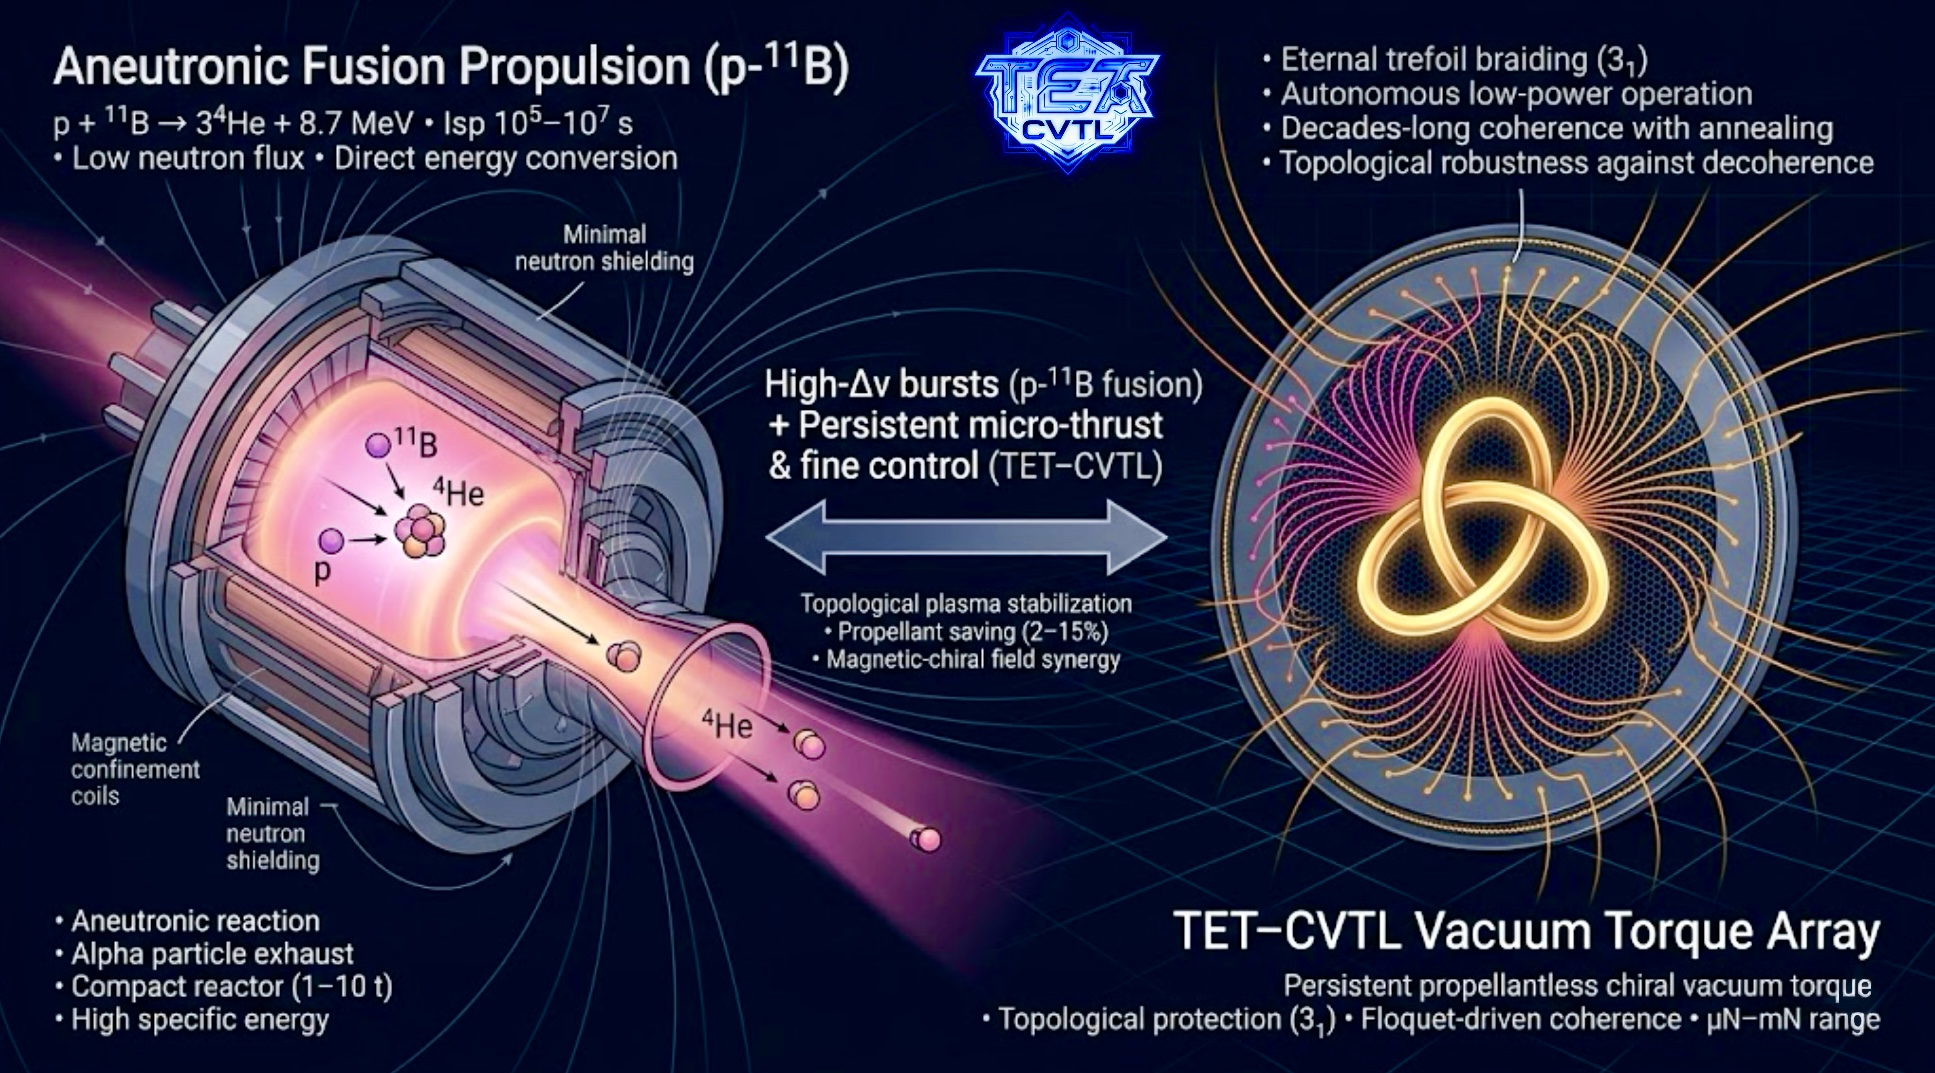
\includegraphics[width=0.95\textwidth]{hybrid_p11b_vacuum.jpg}

\vspace{0.2cm}
\caption{\textbf{Architettura ibrida tra propulsione a fusione aneutronica p-¹¹B e vacuum torque TET--CVTL.} 
Il reattore a fusione p-¹¹B fornisce thrust elevato e $\Delta v$ impulsivo per le manovre principali (escape, Trans-Mars Injection e correzioni mid-course), sfruttando la reazione aneutronica $\mathrm{p} + {}^{11}\mathrm{B} \to 3\,{}^{4}\mathrm{He} + 8.7\,\mathrm{MeV}$. 
L'array TET--CVTL genera invece micro-thrust persistente e propellantless per controllo fine di assetto, momentum dumping e correzioni di traiettoria durante le fasi di cruise. 
La sinergia topologica tra i campi magnetici di confinamento del plasma p-¹¹B e il braiding eterno del trefoil primordiale ($3_1$) consente di stabilizzare instabilità plasmatiche, modulare il thrust vettoriale e ottenere un saving di carburante aneutronico compreso tra il 2\% e il 15\% su missioni di durata 10--50 anni. 
Questa architettura combina l'alta energia specifica della fusione aneutronica con la persistenza e la robustezza topologica del TET--CVTL, rappresentando un passo significativo verso sistemi propulsivi deep-space puliti, efficienti e resilienti.}
\label{fig:p11b_vacuum}
\end{figure}


\vspace{0.3cm}



In sintesi, i lavori del TET Collective sulla catalisi topologica della fusione p-¹¹B combinati con il vacuum torque persistente del TET--CVTL, delineano un’architettura propulsiva pulita, efficiente e resiliente. 

\vspace{0.3cm}


\textbf{La fusione aneutronica p-¹¹B} fornisce la potenza necessaria per le fasi dinamiche della missione, mentre il TET--CVTL garantisce la precisione e la persistenza richieste su scale temporali di decenni. 



\vspace{0.3cm}


Questa integrazione posiziona il sistema come candidato ideale per missioni cargo su Starship, esplorazione del Sistema Solare esterno e futuri precursor verso il mezzo interstellare.








\section{Integrazione con Propulsione a Fusione Inerziale (ICF)}

\vspace{0.2cm}

La propulsione a fusione inerziale (Inertial Confinement Fusion – ICF) si basa sulla compressione rapida e sul riscaldamento di pellet di combustibile (principalmente DT o fuel avanzati come D-³He e p-¹¹B) mediante laser ad alta energia, driver Z-pinch o fasci di ioni pesanti, fino al raggiungimento delle condizioni di ignizione. 


\vspace{0.3cm}



I prodotti di fusione vengono espulsi ad alta velocità attraverso un nozzle magnetico o idrodinamico, generando thrust pulsato. 


\vspace{0.2cm}


Concetti storici come il Vehicle for Interplanetary Transport Applications (VISTA, 1987) e progetti più recenti come HeliosX hanno esplorato questa tecnologia per missioni deep-space con impulso specifico teorico compreso tra $10^4$ e $10^6$\,s e thrust pulsato nell’ordine di 1–100\,N \cite{orth_1987, hyde_1983}.


\vspace{0.3cm}

Gli sviluppi sperimentali degli ultimi anni hanno segnato un progresso significativo. 

\vspace{0.1cm}

L’ignizione scientifica raggiunta al National Ignition Facility (NIF) nel 2022 \cite{abu-shawareb_2022} e i successivi avanzamenti nei programmi di Focused Energy, Xcimer Energy e Marvel Fusion hanno aperto la strada all’utilizzo di fuel aneutronici (D-³He e p-¹¹B) anche in regime inerziale, riducendo drasticamente la produzione di neutroni e i requisiti di shielding.

\vspace{0.3cm}

L’integrazione tra ICF e il framework TET--CVTL rappresenta una sinergia complementare di grande rilevanza. 

\vspace{0.1cm}

Mentre la fusione inerziale eccelle nel fornire potenti burst ad alto $\Delta v$ attraverso micro-esplosioni controllate (frequenza tipica 1–10 Hz), il vacuum torque TET--CVTL garantisce accelerazione continua, propellantless e a bassissima potenza tra un impulso e l’altro.



\vspace{0.3cm}

I principali vantaggi dell’architettura ibrida ICF + TET--CVTL sono:


\vspace{0.2cm}


\begin{itemize}
    \item \textbf{Riduzione del duty cycle e saving di pellet}: il vacuum torque fornisce un contributo persistente di $\Delta v$ tra gli impulsi ICF, riducendo la frequenza di accensione e quindi il consumo di pellet di combustibile. Su missioni di 10–50 anni questo si traduce in un saving stimato tra l’1\% e il 10\% della massa totale di fuel.


\vspace{0.2cm}

    
    \item \textbf{Stabilizzazione topologica delle implosioni}: i campi chirali persistenti generati dal braiding eterno del trefoil primordiale ($3_1$) possono modulare instabilità Rayleigh-Taylor e Richtmyer-Meshkov durante la fase di compressione del pellet, migliorando il guadagno di fusione e la simmetria dell’implosione.


\vspace{0.2cm}

    
    \item \textbf{Controllo fine e momentum management}: il TET--CVTL eccelle nel fornire micro-thrust continuo per attitude control, momentum dumping e correzioni fini di traiettoria, operazioni altrimenti costose in termini di energia e precisione quando affidate solo agli impulsi ICF.


\vspace{0.2cm}


    
    \item \textbf{Robustezza del sistema}: in caso di mancato accensione di un pellet o degrado del driver laser, il vacuum torque funge da sistema di backup autonomo e sempre-on.
\end{itemize}


\vspace{0.3cm}

Per un veicolo di riferimento da 50\,t con propulsione ICF ($I_{sp} \approx 5 \times 10^5$\,s e thrust medio equivalente 10\,N), il contributo cumulativo del vacuum torque TET--CVTL è descritto da:
\begin{equation}
\Delta v_{\text{vac}}(t) = a_{\text{vac}} \cdot \epsilon_{\text{coh}} \cdot t,
\label{eq:dv_vac_icf}
\end{equation}

\vspace{0.3cm}
dove $a_{\text{vac}}$ è l’accelerazione media dell’array ($\sim 10^{-7}$--$10^{-5}$\,m/s²), $\epsilon_{\text{coh}}$ è l’efficienza di coerenza dopo annealing (0,75–0,92), e $t$ è il tempo di missione in anni.

\vspace{0.3cm}

Il saving di pellet risultante può essere stimato come:
\begin{equation}
\text{Saving (\%)} \approx \frac{\Delta v_{\text{vac}}(t)}{\Delta v_{\text{icf}}} \times 100\%,
\label{eq:saving_icf}
\end{equation}
che porta a una riduzione significativa della massa di combustibile da trasportare.


\vspace{0.3cm}

\begin{figure}[H]
\centering
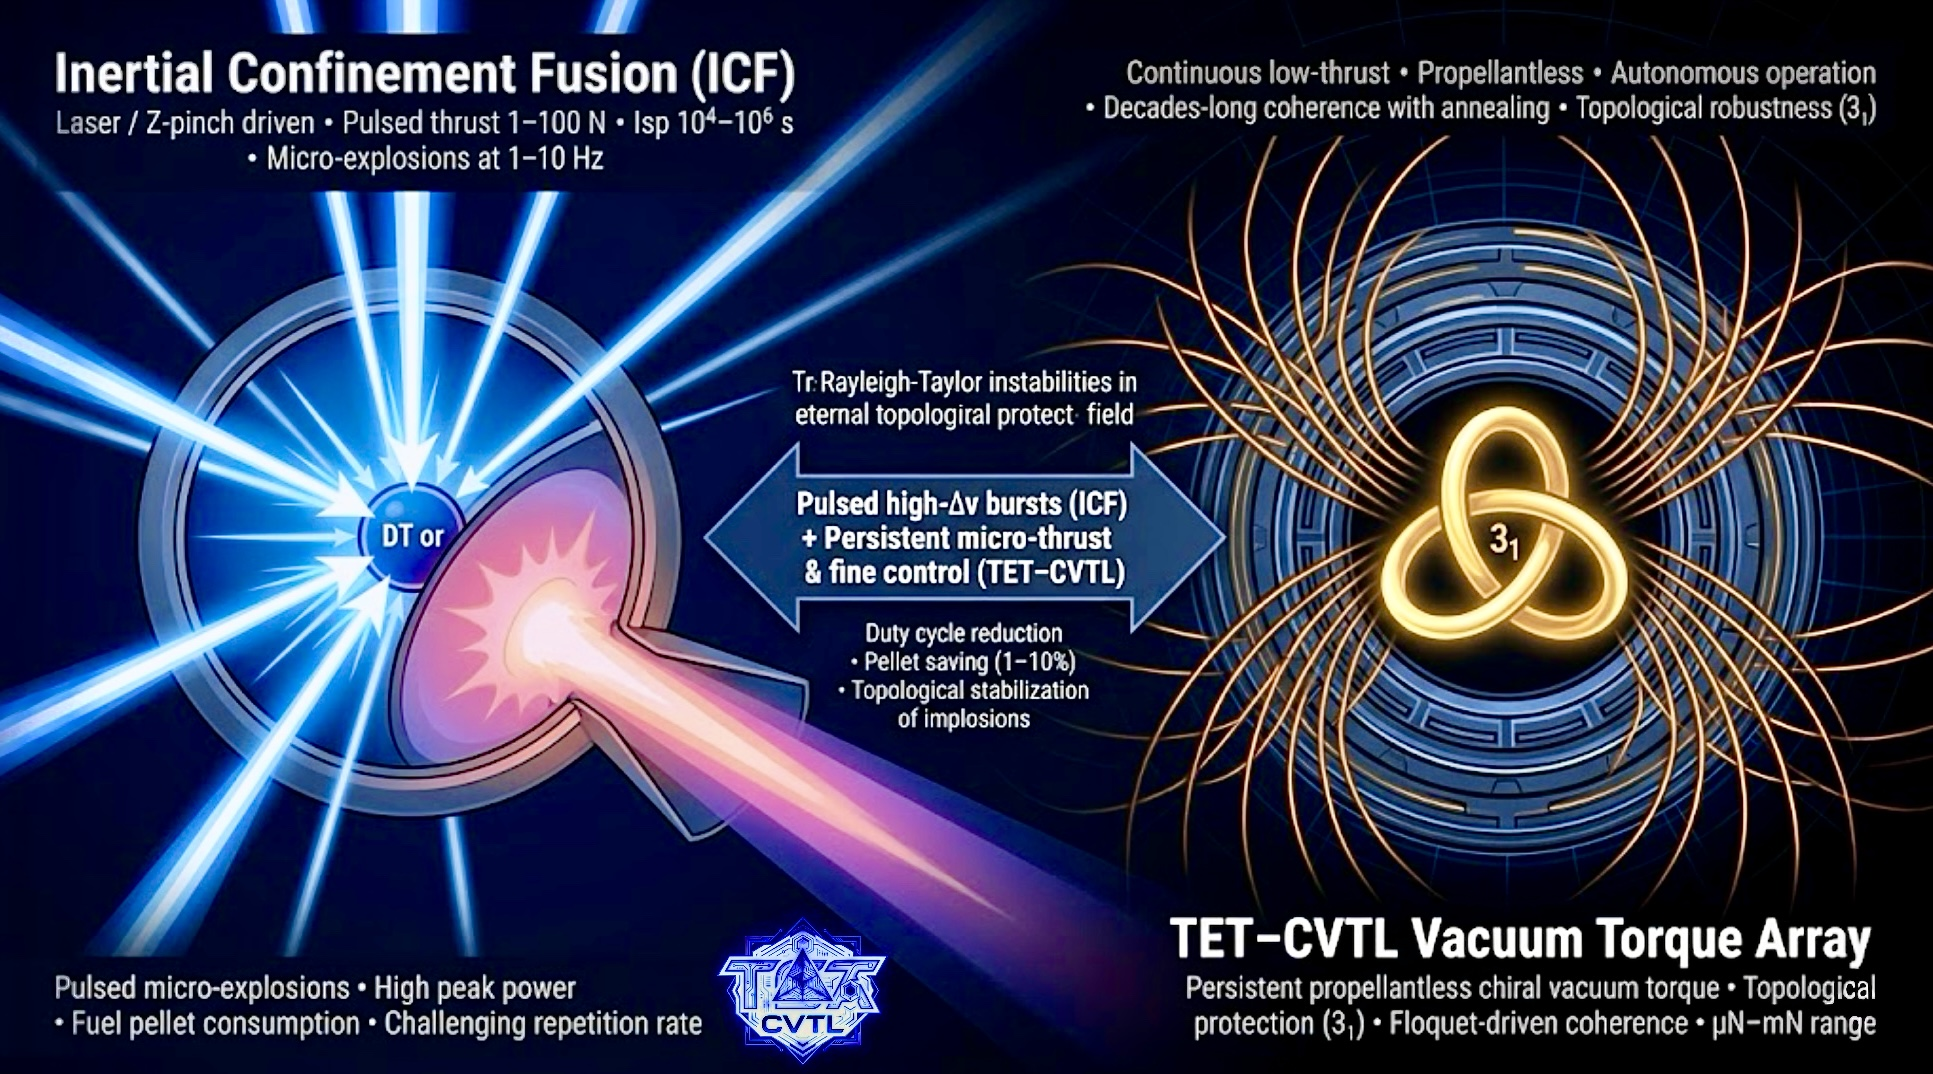
\includegraphics[width=0.95\textwidth]{hybrid_icf_vacuum.jpg}

\vspace{0.2cm}
\caption{\textbf{Architettura ibrida propulsione a fusione inerziale (ICF) + vacuum torque TET--CVTL.} 
Il sistema ICF genera thrust pulsato ad alto $\Delta v$ attraverso micro-esplosioni controllate di pellet di combustibile, mentre l’array TET--CVTL fornisce micro-thrust persistente e propellantless per controllo fine, attitude control e momentum dumping tra gli impulsi. 
La sinergia topologica tra la dinamica di implosione e il braiding eterno del trefoil primordiale ($3_1$) può migliorare la stabilità delle implosioni e l’efficienza complessiva del sistema.}
\label{fig:icf_vacuum}
\end{figure}

Questa integrazione trasforma la propulsione inerziale da sistema pulsato e ad alto consumo di energia in un’architettura più efficiente, resiliente e adatta a missioni di lunga durata.










\section{Integrazione con Propulsione a Fusione Catalizzata da Muoni (MCF)}


\vspace{0.2cm}

La fusione catalizzata da muoni (Muon-Catalyzed Fusion -- MCF) rappresenta un approccio affascinante per superare la barriera coulombiana tra nuclei leggeri. 

\vspace{0.3cm}

Sfruttando muoni negativi ($\mu^-$), la MCF permette reazioni di fusione DT o D-D a temperature criogeniche o prossime alla temperatura ambiente, riducendo drasticamente l'energia di attivazione richiesta.

\vspace{0.3cm}

Un singolo muone può catalizzare teoricamente centinaia di fusioni prima di decadere (vita media $\tau_\mu \approx 2.2\,\mu$s). In pratica, il numero di cicli catalitici per muone è attualmente limitato a circa 150 a causa del fenomeno di ``sticking'' (intrappolamento del muone nell'elio prodotto dalla fusione, con probabilità effettiva intorno allo 0.3--0.7\% dopo riattivazione) \cite{breunlich_1989, rafelski_2020}.



\vspace{0.3cm}




Nonostante il potenziale concettuale, nel 2026 lo stato tecnologico della MCF rimane sfidante: la produzione efficiente di muoni richiede acceleratori di particelle ad alta intensità con consumi energetici nell'ordine dei megawatt per generare flussi di $10^6$--$10^9$ muoni al secondo. L'efficienza complessiva del ciclo catalitico è ancora troppo bassa per applicazioni pratiche su scala propulsiva.


\vspace{0.2cm}


\begin{figure}[H]
\centering
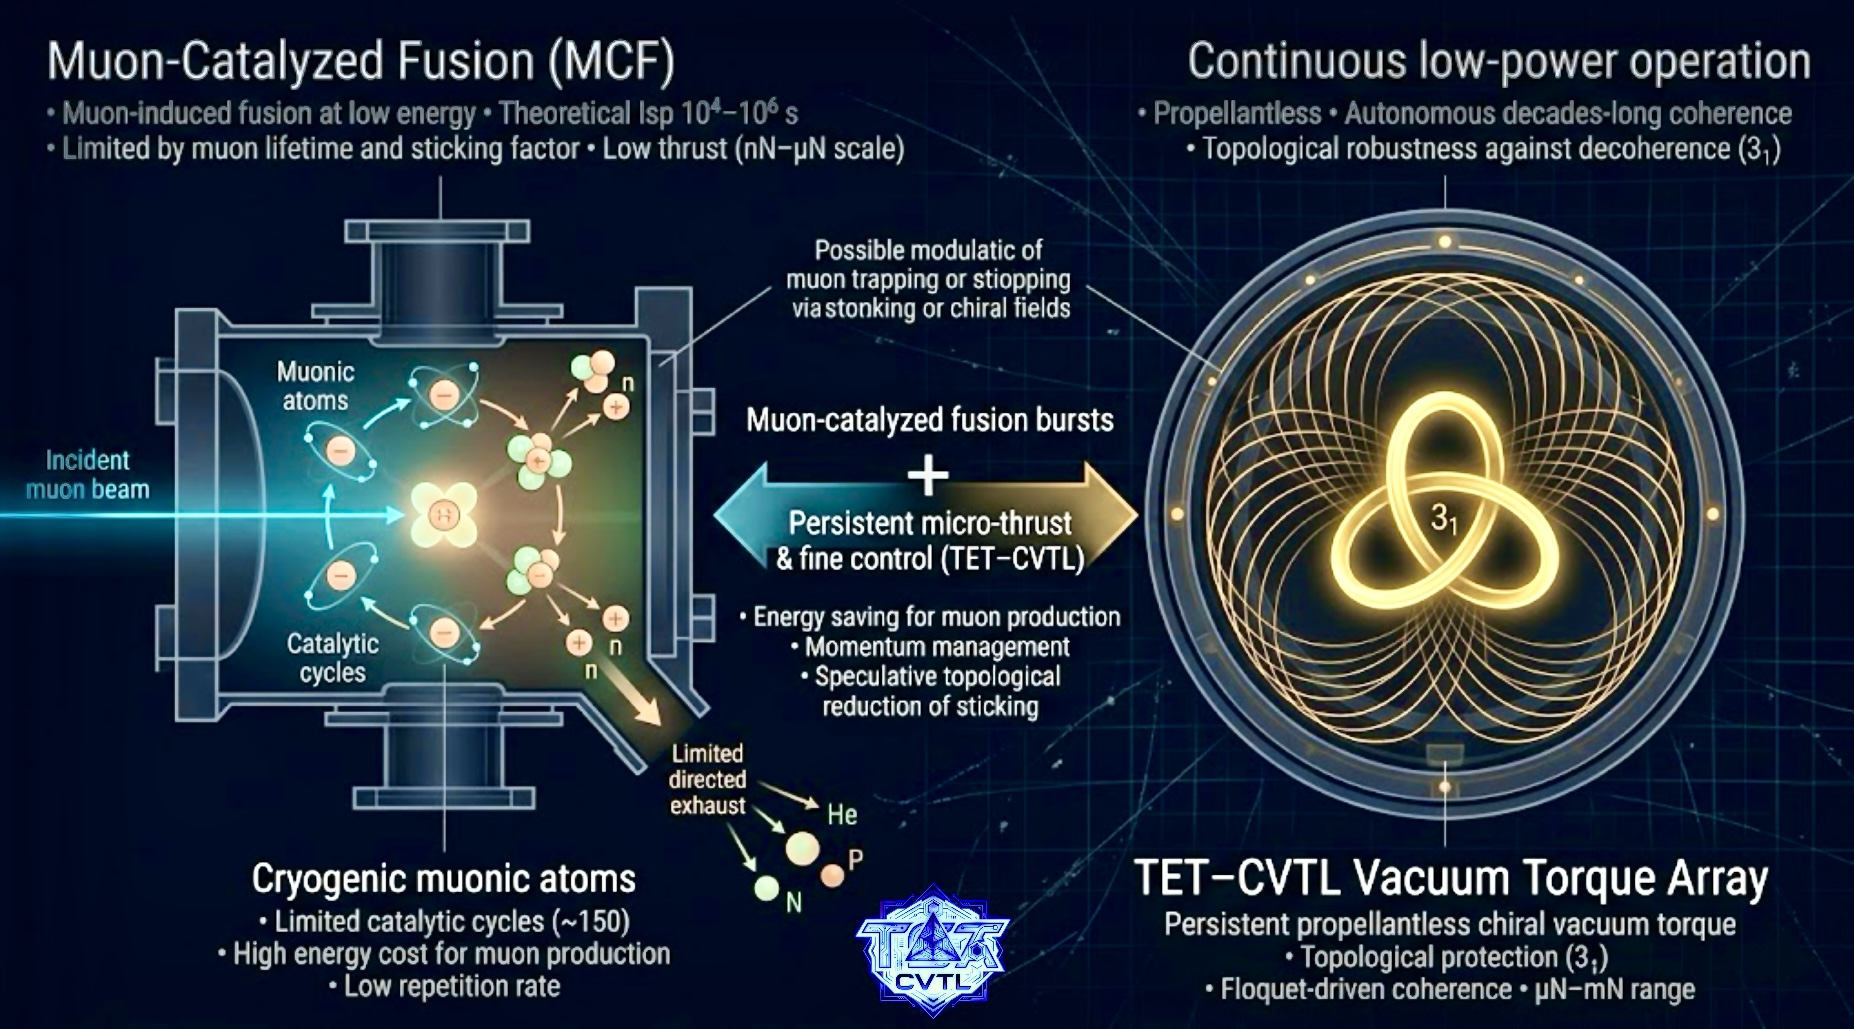
\includegraphics[width=0.95\textwidth]{hybrid_mcf_vacuum.jpg}
\vspace{0.2cm}
\caption{\textbf{Architettura ibrida propulsione a fusione catalizzata da muoni (MCF) + vacuum torque TET--CVTL.} 
Il sistema MCF genera thrust attraverso cicli catalitici di fusione a bassa energia, mentre il TET--CVTL fornisce micro-thrust persistente e propellantless per controllo fine e momentum management durante le lunghissime fasi di cruise. 
La protezione topologica del trefoil primordiale ($3_1$) garantisce operatività autonoma anche in presenza di fluttuazioni nella produzione di muoni.}
\label{fig:mcf_vacuum}
\end{figure}




\vspace{0.3cm}




\vspace{0.4cm}

\subsection{Sinergie con il framework TET--CVTL}

\vspace{0.2cm}

L'integrazione della MCF con il paradigma TET--CVTL offre una soluzione ibrida promettente per mitigare le limitazioni energetiche e operative della fusione muon-catalizzata. 

\vspace{0.3cm}


Il vacuum torque chiral TET--CVTL funge da sistema propulsivo ausiliario propellantless a bassissimo consumo, permettendo di ottimizzare l'utilizzo del sistema MCF principale.


\vspace{0.4cm}

I principali punti di sinergia sono:

\vspace{0.2cm}

\begin{itemize}
    \item \textbf{Riduzione del consumo energetico}: il torque dal vuoto fornisce un micro-thrust continuo e persistente senza richiedere produzione costante di muoni. Ciò consente di attivare il sistema MCF solo durante fasi di accelerazione impulsive o correzioni di traiettoria maggiori, potenzialmente riducendo il fabbisogno energetico per la generazione di muoni del 5--20\% su missioni di lunghissima durata.

    \vspace{0.2cm}
    
    \item \textbf{Controllo fine e ridondanza}: il TET--CVTL garantisce attitude control preciso, momentum dumping e piccole correzioni orbitali anche in caso di interruzione temporanea del ciclo catalitico MCF, aumentando la robustezza complessiva del sistema propulsivo.

    \vspace{0.2cm}
    
    \item \textbf{Sinergia topologica sul fenomeno di sticking (speculativa)}: il nodo trefoil primordiale ($T_{2,3}$ o $3_1$), con la sua protezione topologica eterna e il braiding anyonico non-abeliano, potrebbe influenzare positivamente la dinamica dei muoni nel regime post-fusione. 

    

\vspace{0.4cm}


      Dopo la reazione DT, il muone ha una probabilità non trascurabile di rimanere intrappolato nello ione $\mu\alpha^+$ (muonic helium). 
      
      \vspace{0.5cm}
      
      Nel paradigma TET--CVTL, i campi chirali persistenti e la coerenza topologica indotta dal trefoil potrebbero modulare questo processo attraverso due meccanismi concettuali:

      \vspace{0.2cm}
      
      \begin{enumerate}
          \item \textbf{Coerenza collettiva e riattivazione assistita}: il braiding anyonico mediato dal trefoil introduce una fase topologica non-locale che potrebbe stabilizzare stati quantistici collettivi nel plasma muónico. Questo effetto potrebbe aumentare la probabilità di riattivazione (stripping) del muone dall'ione $\mu\alpha^+$, riducendo efficacemente il fattore di sticking. Matematicamente, tale modulazione potrebbe essere descritta da un termine addizionale nella probabilità di sticking:
          
          \begin{equation}
          P_{\text{stick,eff}} \approx P_{\text{stick,0}} \left(1 - \eta \, l(K) \, \epsilon_{\text{coh}}\right),
          \label{eq:sticking_trefoil}
          \end{equation}

          
\vspace{0.2cm}

          
          dove \(P_{\text{stick,0}}\) è la probabilità standard ($\sim 0.6\%$), \(l(K)=3\) è il linking number del trefoil, ed \(\eta\) è un fattore di accoppiamento tra la chiralità topologica e la dinamica muonica (da determinare teoricamente o sperimentalmente).


\vspace{0.3cm}
          
          \item \textbf{Modulazione chirale del potenziale di legame}: la geometria chirale persistente del trefoil potrebbe indurre una leggera anisotropia o una torsione topologica nel potenziale Coulombiano effettivo visto dal muone nello ione $\mu\alpha^+$. Questo potrebbe favorire stati di maggiore energia o stati di scattering che facilitano il distacco del muone, analogamente a come il torque Casimir estrae momento angolare dal vuoto.
      \end{enumerate}


      \vspace{0.2cm}
      
      Tale ipotesi rimane altamente speculativa e richiede modelli quantistici avanzati (ad esempio basati su Floquet-Lindblad o simulazioni QuTiP con hamiltoniane effective topologiche). 

\vspace{0.4cm}


      
      Tuttavia, se confermata, potrebbe aumentare significativamente il numero di fusioni per muone (da $\sim$150 a valori superiori a 300--500), migliorando drasticamente l'economia energetica della MCF e rendendo l'architettura ibrida MCF + TET--CVTL particolarmente attraente per missioni deep-space ultra-lunghe.
\end{itemize}


\vspace{0.4cm}

\subsection{Contributo propulsivo su missioni di lunghissima durata}

\vspace{0.2cm}

Per un veicolo di riferimento di massa 10\,t equipaggiato con propulsione MCF ($I_{sp} \approx 10^5$\,s e thrust medio equivalente $\sim 1$\,mN), il contributo cumulativo del vacuum torque TET--CVTL durante la fase di cruise è descritto da:

\begin{equation}
\Delta v_{\text{vac}}(t) = a_{\text{vac}} \cdot \epsilon_{\text{coh}} \cdot t,
\label{eq:dv_vac_mcf}
\end{equation}

\vspace{0.2cm}

dove \(a_{\text{vac}}\) è l'accelerazione specifica fornita dal torque Casimir chiral, ed \(\epsilon_{\text{coh}}\) rappresenta il fattore di coerenza topologica mantenuta tramite annealing termico adattivo.


\vspace{0.2cm}

Su missioni di durata superiore a 100 anni (es. sonde interstellari o missioni di esplorazione outer solar system), questo contributo propellantless diventa strategicamente rilevante. 


\vspace{0.2cm}


Permette di mantenere una precisione di traiettoria elevata con consumo energetico minimo, riducendo drasticamente il tempo di accensione del sistema MCF e allungando la vita utile complessiva della missione.

\vspace{0.4cm}

L'architettura ibrida MCF + TET--CVTL rappresenta quindi un passo naturale verso sistemi propulsivi sostenibili e fault-tolerant per l'esplorazione deep-space, combinando l'alto impulso specifico della fusione muon-catalizzata con l'estrazione topologica di momento angolare dal vuoto quantistico mediata dal trefoil primordiale.



\vspace{0.3cm}



Sebbene la MCF rimanga una tecnologia di frontiera con sfide significative, la sua integrazione con il vacuum torque TET--CVTL potrebbe trasformare un concetto energeticamente inefficiente in un sistema ibrido più realistico per missioni interstellari di lunghissima durata.

















\section{Integrazione con Vela Elettrica Avanzata (E-sail e varianti)}

\vspace{0.2cm}

La vela elettrica avanzata (Electric Sail – E-sail) rappresenta un’evoluzione significativa del concetto originale proposto da Pekka Janhunen nel 2004. 


\vspace{0.3cm}


Il principio di funzionamento si basa su una serie di lunghi tethers conduttori caricati positivamente ad alto voltaggio che interagiscono con il vento solare. Gli ioni del plasma solare (principalmente protoni) vengono deflessi dal campo elettrico generato intorno ai tethers, producendo una forza di reazione netta che genera thrust senza alcun consumo di propellente \cite{janhunen_2004}.


\vspace{0.3cm}

Rispetto al concetto iniziale, le varianti recenti (2025–2026), sviluppate da Aurora Propulsion Technologies e supportate dall’European Space Agency, introducono importanti miglioramenti tecnologici:

\vspace{0.2cm}


\begin{itemize}
    \item \textbf{Multi-tether dinamici}: configurazioni con decine di tethers di lunghezza fino a 100\,km, in grado di modulare attivamente la tensione e la geometria durante il volo;

\vspace{0.2cm}

    
    \item \textbf{Modulazione attiva del campo elettrico}: controllo in tempo reale della sheath plasma attorno ai tethers per ottimizzare il thrust e consentire un rudimentale thrust vectoring;


\vspace{0.2cm}
    
    \item \textbf{Sistemi di controllo avanzato}: algoritmi di stabilizzazione e adattamento dinamico alla variabilità del vento solare, migliorando l’efficienza complessiva e la manovrabilità.
\end{itemize}

\vspace{0.3cm}

Queste evoluzioni consentono di ottenere prestazioni significativamente superiori rispetto al design originale. 


\vspace{0.4cm}


Il thrust tipico di un sistema E-sail avanzato varia tra 0,1 e 100\,mN per un insieme di tethers di lunghezza complessiva 10–100\,km a 1\,UA, con un impulso specifico virtualmente infinito ($I_{sp} \to \infty$) e una massa del sistema compresa tra 50 e 500\,kg (inclusi tethers, generatore di alta tensione ed elettronica di controllo).


\vspace{0.3cm}

Nonostante i progressi, l’E-sail mantiene limitazioni intrinseche legate alla forte dipendenza dal vento solare: il thrust decresce con il quadrato della distanza dal Sole ($\propto 1/r^2$) e la direzione è prevalentemente radiale (opposta al flusso del plasma in arrivo), rendendo difficili le manovre out-of-plane o tangenziali senza sistemi ausiliari.


\vspace{0.5cm}

Le caratteristiche principali dei sistemi E-sail avanzati sono:


\vspace{0.2cm}

\begin{itemize}
    \item Thrust: 0,1–100 mN per sistema con tether totali di 10–100 km a 1 AU;

\vspace{0.2cm}
    
    \item Impulso specifico: $I_{sp} \to \infty$ (propellantless);

    
\vspace{0.2cm}



    \item Massa del sistema: 50–500 kg (tethers + generatore di carica + elettronica di controllo);

\vspace{0.2cm}
    
    \item Vantaggi: thrust continuo dal vento solare, scalabilità con lunghezza dei tether;


\vspace{0.2cm}
    
    \item Limitazioni: thrust decresce con il quadrato della distanza dal Sole ($\propto 1/r^2$), direzione prevalentemente radiale (anti-vento solare), e necessità di mantenere carica elevata sui tether.
\end{itemize}


\vspace{0.4cm}

L’integrazione con il framework TET--CVTL crea una sinergia complementare di grande potenza. 


\vspace{0.2cm}

Mentre l’E-sail fornisce thrust radiale principale sfruttando il vento solare, il vacuum torque TET--CVTL genera una componente chirale e out-of-plane indipendente dalla direzione del plasma solare.

\vspace{0.2cm}




\begin{figure}[H]
\centering
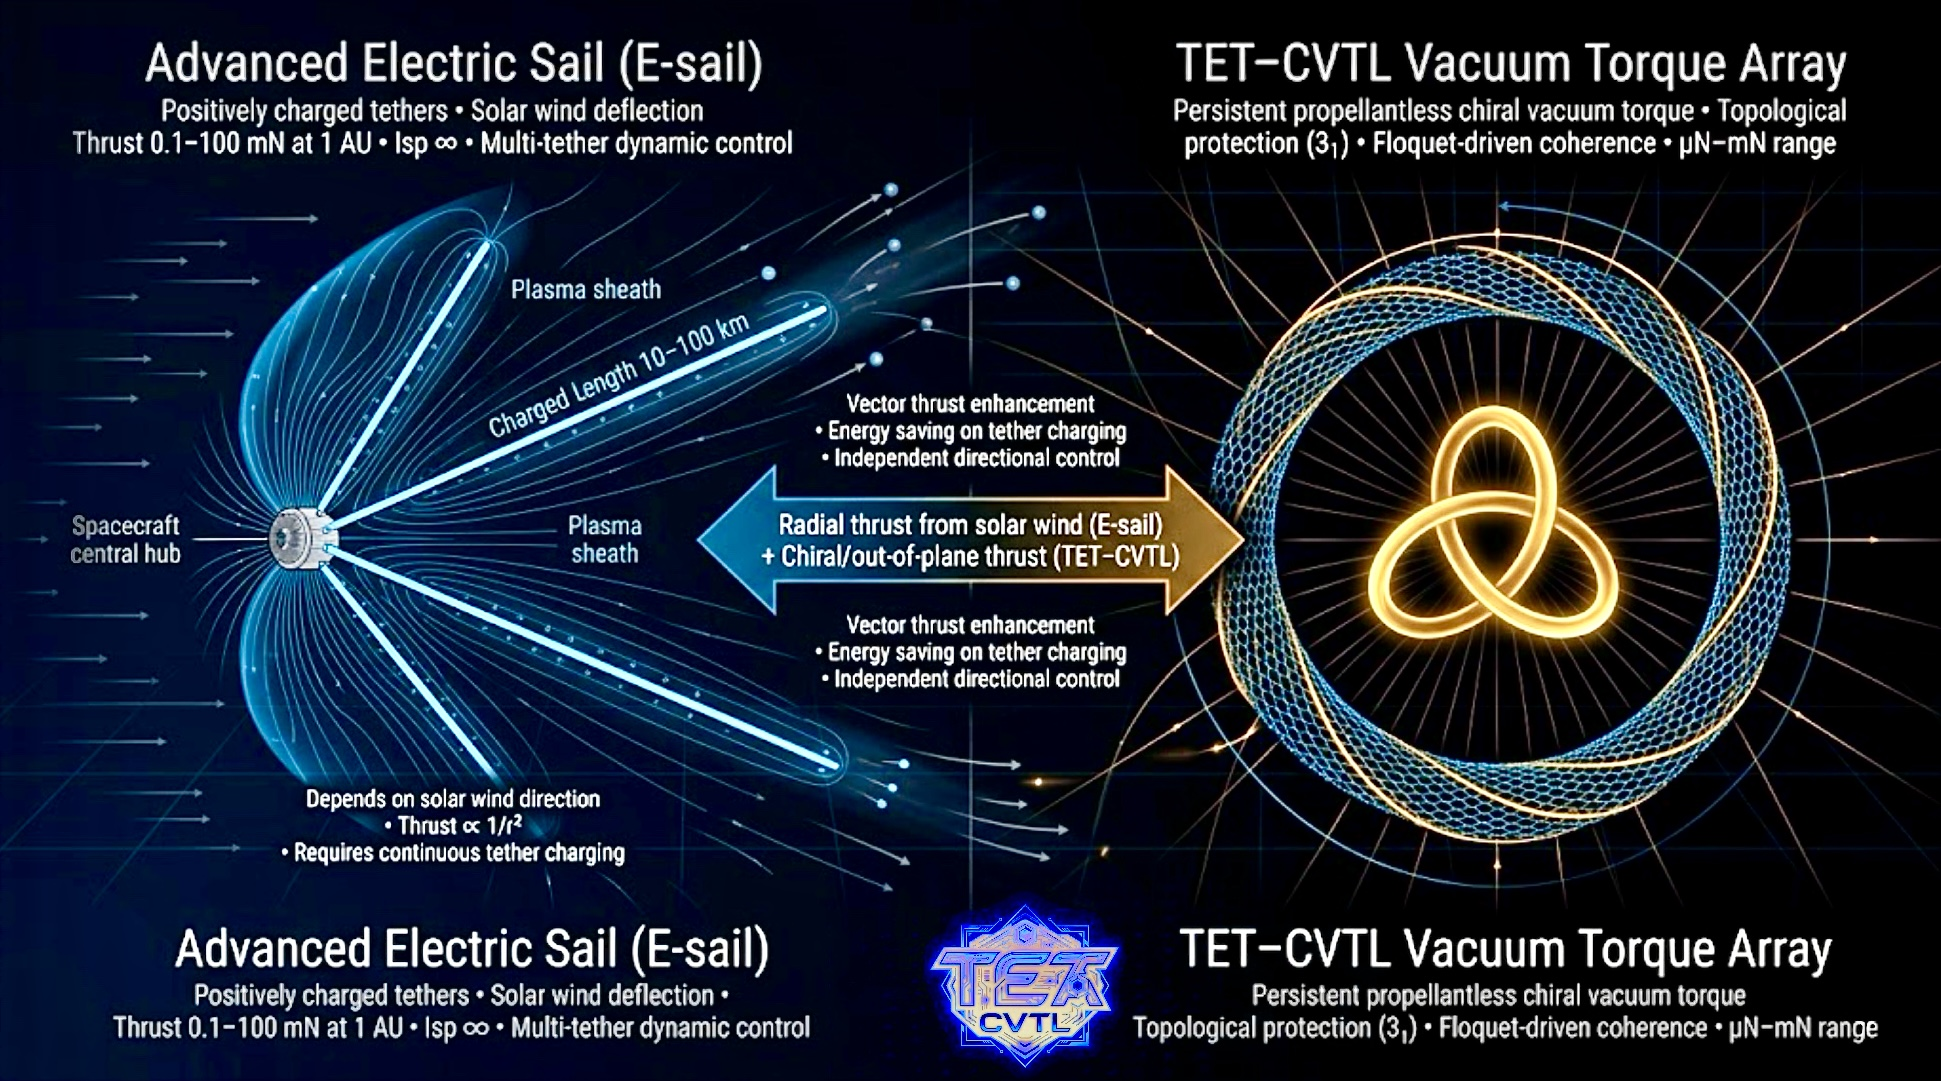
\includegraphics[width=0.95\textwidth]{hybrid_esail_vacuum.jpg}
\vspace{0.2cm}
\caption{\textbf{Architettura ibrida vela elettrica avanzata (E-sail) + vacuum torque TET--CVTL.} 
L’E-sail genera thrust radiale sfruttando il vento solare attraverso tethers caricati positivamente, mentre il TET--CVTL fornisce componente chirale e out-of-plane indipendente, consentendo correzioni tangenziali e attitude control con elevata precisione. 
Questa sinergia supera le limitazioni direzionali dell’E-sail e riduce il fabbisogno energetico per il mantenimento della carica sui tether.}
\label{fig:esail_vacuum}
\end{figure}









\vspace{0.3cm}

I vantaggi principali dell’architettura ibrida E-sail + TET--CVTL sono:


\vspace{0.2cm}



\begin{itemize}
    \item \textbf{Superamento della limitazione direzionale}: il vacuum torque fornisce spinta tangenziale e out-of-plane, permettendo manovre che l’E-sail da sola non può effettuare efficientemente.


\vspace{0.2cm}

    
    \item \textbf{Riduzione del consumo energetico}: il TET--CVTL riduce la necessità di mantenere carica elevata sui tether per correzioni fini, con conseguente saving di potenza per il sistema di charging.



\vspace{0.2cm}

    
    \item \textbf{Sinergia elettrica-topologica}: i forti campi elettrici generati dall’E-sail potrebbero essere sfruttati per modulare o amplificare il torque chirale del TET--CVTL, creando un effetto di coupling tra sheath plasma e braiding topologico.

    
\vspace{0.2cm}



    \item \textbf{Maggiore flessibilità missioni}: combinazione ideale per spiral-out da 1 AU verso il Sistema Solare esterno o per missioni di mantenimento di costellazioni cis-lunari.
\end{itemize}

\vspace{0.3cm}

Una stima quantitativa per un E-sail avanzata con tether totali di 50 km a 5 AU mostra un thrust tipico di 0,05–0,5 mN. L’array TET--CVTL (1–10 m²) contribuisce con 1–10 mN, portando a un aumento del thrust vettoriale totale del 200–2000\%, con una manovrabilità significativamente superiore.





\vspace{0.5cm}




\section{Integrazione con Vela Magnetica (MagSail)}

\vspace{0.2cm}

La vela magnetica (Magnetic Sail o MagSail) sfrutta l’interazione tra un intenso campo magnetico generato a bordo e il vento solare (o il plasma interstellare) per produrre thrust senza consumo di propellente. 


\vspace{0.3cm}


Il concetto, originariamente proposto da Robert Zubrin negli anni ’90, si basa sulla deflessione delle particelle cariche del plasma da parte di un campo magnetico creato da un grande loop superconduttore o da un solenoide. 

\vspace{0.2cm}


Questa deflessione genera una forza di reazione che accelera il veicolo in modo analogo a una vela che intercetta il vento.

\vspace{0.2cm}

Sviluppi successivi hanno notevolmente migliorato la fattibilità del concetto grazie all’impiego di superconduttori ad alta temperatura, in particolare YBCO (Yttrium Barium Copper Oxide) e MgB$_2$ (Magnesio Diboruro). 

\vspace{0.2cm}


Questi materiali permettono di generare campi magnetici intensi, nell’intervallo 0,01–1\,T, riducendo drasticamente sia la massa del sistema sia i requisiti criogenici rispetto alle soluzioni basate su superconduttori tradizionali a bassa temperatura.


\vspace{0.2cm}

Il sistema offre un impulso specifico virtualmente infinito ($I_{sp} \to \infty$) e un thrust continuo. 


\vspace{0.2cm}

In condizioni tipiche a 1\,UA, un MagSail con loop di diametro compreso tra 1 e 10\,km è in grado di produrre un thrust tra 0,1 e 10\,mN, a seconda dell’intensità del campo magnetico e della densità del vento solare.

\vspace{0.2cm}

Le caratteristiche principali della MagSail sono:


\vspace{0.2cm}


\begin{itemize}
    \item Thrust dipendente dalla densità e velocità del plasma esterno (vento solare o interstellare);

    
\vspace{0.2cm}



    \item Direzione prevalentemente radiale (opposta al flusso del plasma);


\vspace{0.2cm}
    
    \item Necessità di criogenia per mantenere i superconduttori in stato superconduttivo;


\vspace{0.2cm}

    
    \item Scalabilità con la dimensione del loop e l’intensità del campo B.
\end{itemize}



Nonostante i suoi vantaggi, la vela magnetica presenta limitazioni intrinseche: il thrust decresce con il quadrato della distanza dal Sole ($\propto 1/r^2$), la direzione è fortemente vincolata al flusso del plasma in arrivo, e il sistema richiede una massa non trascurabile per il loop superconduttore e il sistema di raffreddamento.


\vspace{0.2cm}

Le caratteristiche principali dei sistemi MagSail attuali sono:
\begin{itemize}
    \item Thrust: 0,1–10 mN per loop di 1–10 km di diametro a 1 AU (dipendente dall’intensità del campo B, tipicamente 0,01–1 T);
    \item Impulso specifico: $I_{sp} \to \infty$ (propellantless);
    \item Massa del sistema: 10–1000 kg (loop superconduttore + criogenia);
    \item Vantaggi: thrust continuo dal vento solare/plasma, scalabilità con dimensione del loop;
    \item Limitazioni: thrust decresce con $1/r^2$ allontanandosi dal Sole, direzione prevalentemente opposta al vento solare, e necessità di criogenia per mantenere i superconduttori in stato superconduttivo.
\end{itemize}




\begin{figure}[H]
\centering
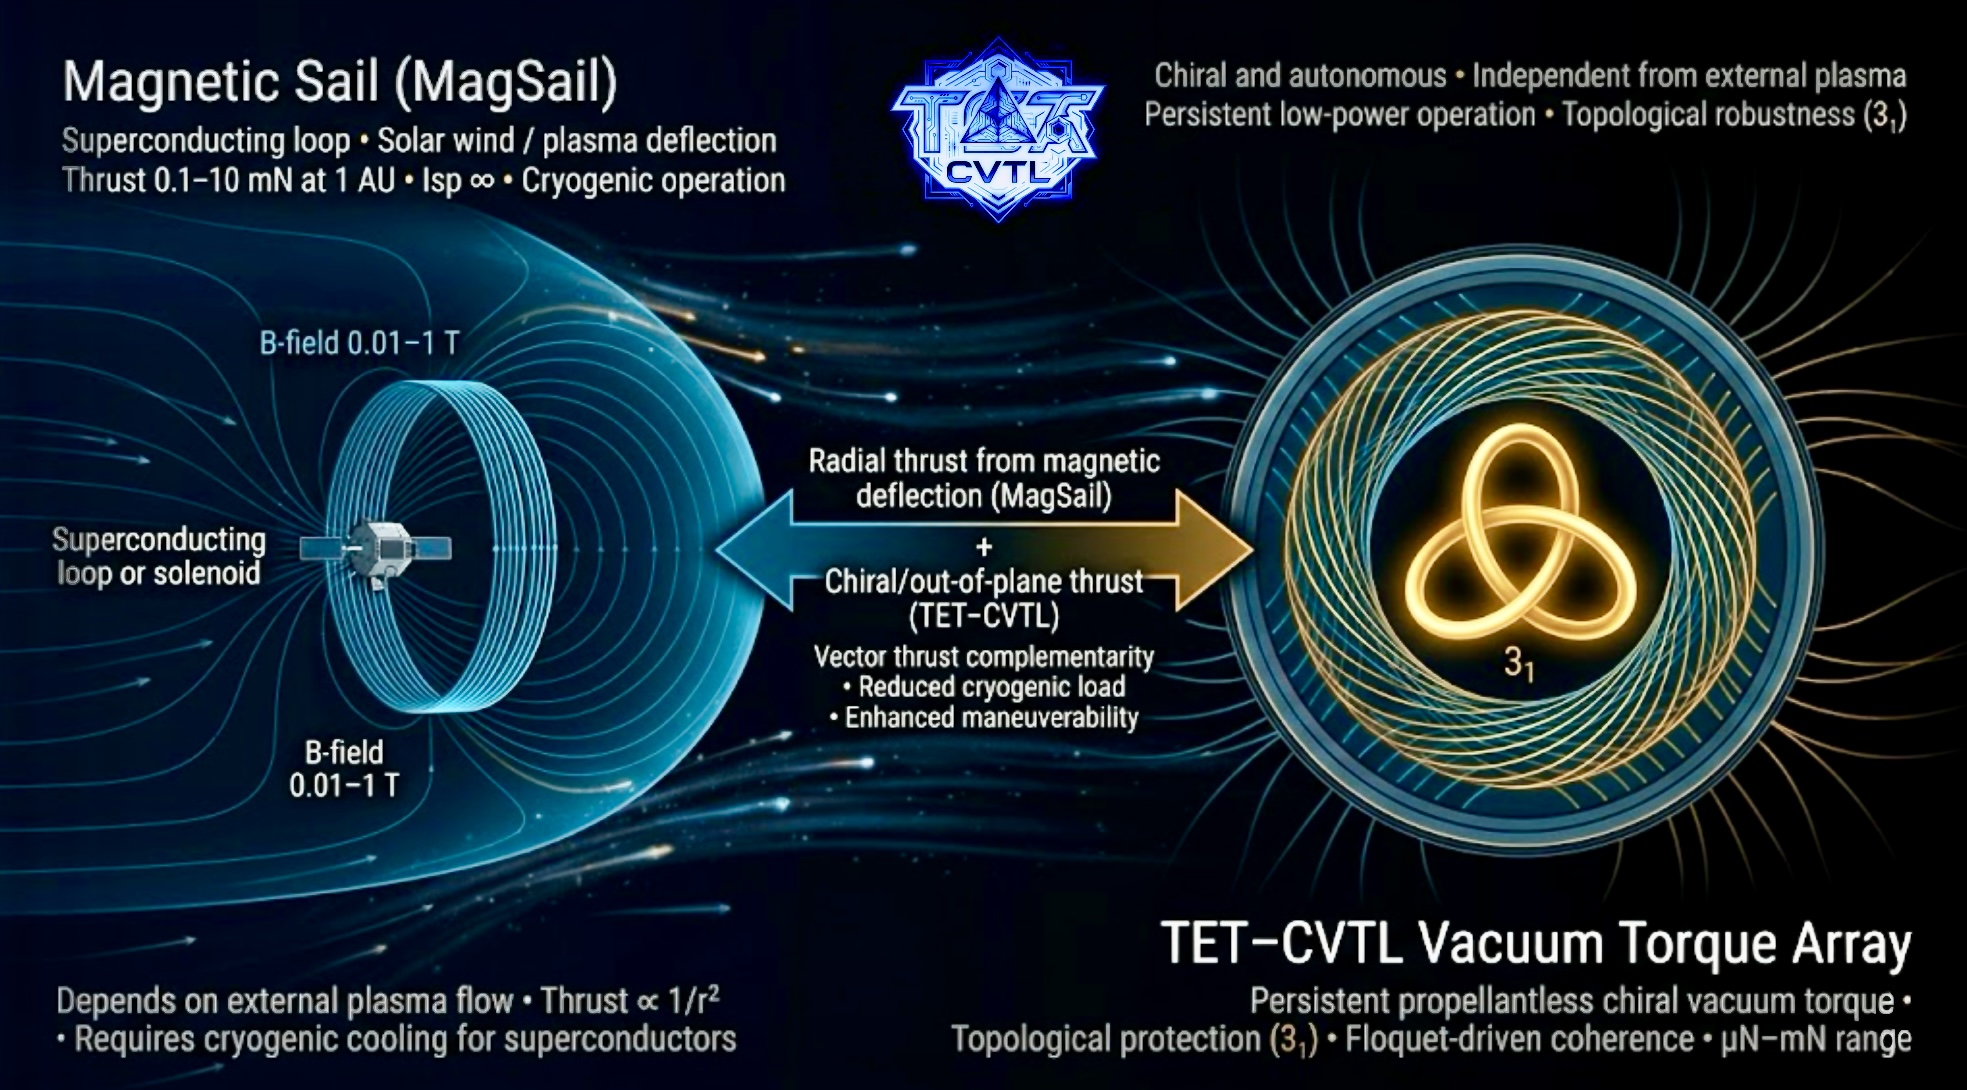
\includegraphics[width=0.95\textwidth]{hybrid_magsail_vacuum.jpg}
\caption{\textbf{Architettura ibrida vela magnetica (MagSail) + vacuum torque TET--CVTL.} 
La vela magnetica genera thrust radiale deflettendo il vento solare o il plasma interstellare tramite un forte campo magnetico superconduttore, mentre il TET--CVTL fornisce componente chirale autonoma e persistente per correzioni tangenziali, out-of-plane e attitude control.}
\label{fig:magsail_vacuum}
\end{figure}

Questa sinergia riduce la dipendenza dal vento solare e migliora significativamente la manovrabilità complessiva del sistema.

\vspace{0.2cm}



L’integrazione con il framework TET--CVTL offre una complementarità vettoriale e operativa estremamente interessante. Mentre la vela magnetica fornisce thrust radiale principale (anti-vento solare), il vacuum torque TET--CVTL genera una componente chirale indipendente e controllabile.


\vspace{0.3cm}

I vantaggi principali dell’architettura ibrida MagSail + TET--CVTL sono:

\vspace{0.2cm}


\begin{itemize}
    \item \textbf{Complementarietà direzionale}: il vacuum torque fornisce spinta tangenziale e out-of-plane, superando la limitazione intrinseca della MagSail di spingere solo nella direzione opposta al vento solare.


\vspace{0.2cm}

    


    \item \textbf{Riduzione della complessità criogenica}: il TET--CVTL opera a temperatura ambiente e non richiede criogenia, alleggerendo il carico termico sul sistema superconduttore della MagSail.


\vspace{0.2cm}


    
    \item \textbf{Momentum dumping e attitude control}: il torque chirale non-locale è ideale per scaricare momento angolare accumulato senza consumo di energia o propellente.


\vspace{0.2cm}

    
    \item \textbf{Sinergia campi magnetici}: i forti campi generati dalla MagSail possono interagire con il braiding topologico del TET--CVTL, potenzialmente amplificando o modulando il torque chirale.
\end{itemize}

\vspace{0.3cm}

Una stima per una MagSail con loop di 5 km di diametro a 5 AU indica un thrust tipico di 0,1–1 mN. L’array TET--CVTL (1–10 m²) contribuisce con 1–10 mN, portando a un aumento del thrust vettoriale totale del 50–1000\%, con una flessibilità direzionale notevolmente superiore.







\vspace{0.5cm}




\section{Integrazione con Altre Tecnologie Esotiche}

\vspace{0.2cm}

\subsection{Propulsione a fusione inerziale avanzata e Project Daedalus}


\vspace{0.2cm}

Project Daedalus (British Interplanetary Society, 1973–1978) rimane il riferimento storico fondamentale per la propulsione interstellare robotica. 

\vspace{0.3cm}

Il concept prevedeva un veicolo a due stadi di massa complessiva circa 50\,000 tonnellate, spinto da propulsione a fusione inerziale (ICF) con pellet di deuterio ed elio-3 (D-³He). 


\vspace{0.2cm}


Il sistema generava impulsi pulsati ad altissima energia (frequenza ~250 Hz nello stadio I), raggiungendo una velocità di crociera di circa 0,12$c$ per un flyby della stella di Barnard in circa 50 anni \cite{bond_1978}.

\vspace{0.3cm}

Le caratteristiche principali del design originale includevano thrust per impulso dell’ordine di $10^7$\,N (stadio I) e $10^6$\,N (stadio II), impulso specifico $I_{sp} \approx 10^6$\,s ottenuto mediante espulsione diretta del plasma attraverso un nozzle magnetico superconduttore, e un payload scientifico di circa 500\,kg. L’accelerazione media era compresa tra 0,01 e 0,1$g$, con una fase di accelerazione totale di circa 7 anni.


\vspace{0.4cm}

L’integrazione con il framework TET--CVTL offre un complemento naturale e strategico al concetto Daedalus. 

\vspace{0.4cm}


Mentre la propulsione ICF fornisce i potenti burst necessari per raggiungere velocità relativistiche, il vacuum torque TET--CVTL può agire come sistema ausiliario persistente tra un impulso e l’altro, fornendo:
\begin{itemize}
    \item Controllo fine di assetto e momentum dumping durante le lunghe fasi di coast;
    \item Riduzione del duty cycle del sistema ICF, con conseguente saving di pellet stimato tra l’1\% e il 5\% su una missione di 50 anni;
    \item Stabilizzazione topologica delle implosioni dei pellet e modulazione del nozzle magnetico tramite i campi chirali persistenti generati dal braiding eterno del trefoil primordiale ($3_1$).
\end{itemize}

\vspace{0.2cm}

\begin{figure}[H]
\centering
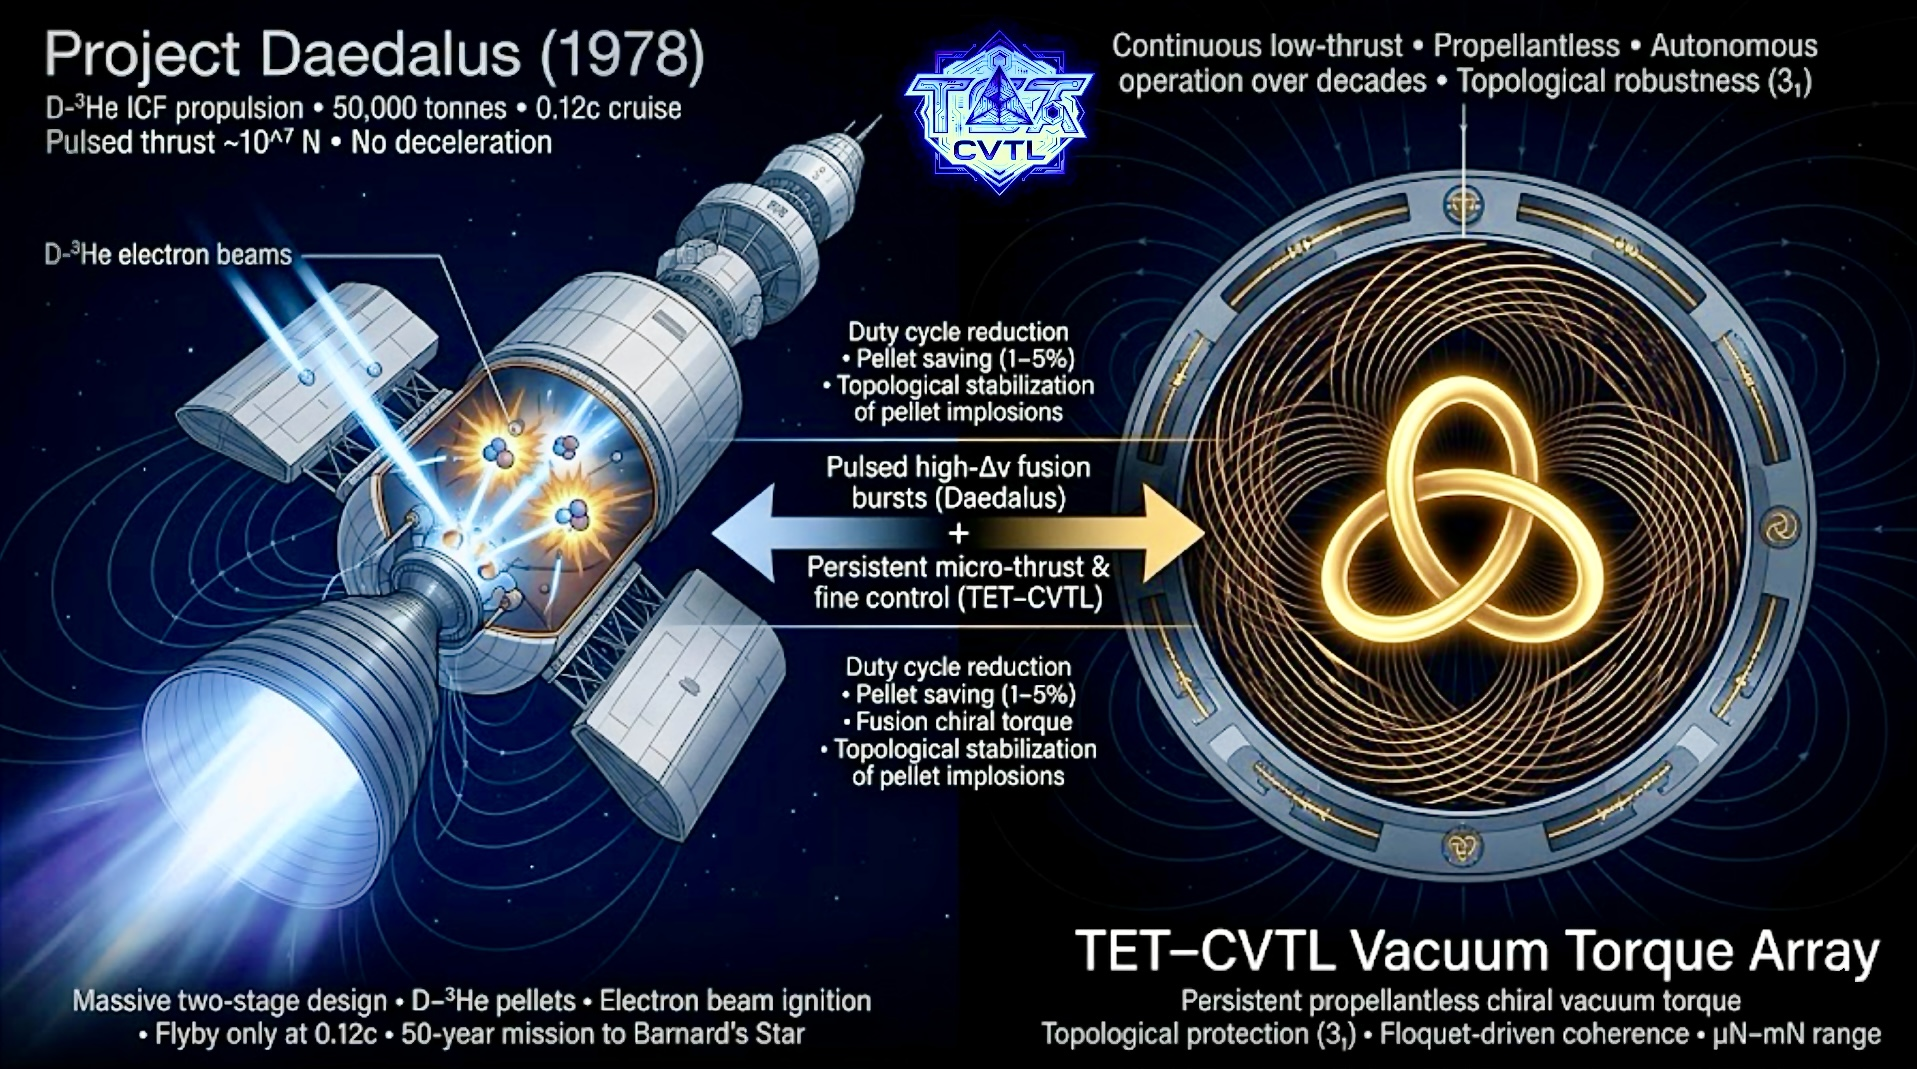
\includegraphics[width=0.95\textwidth]{hybrid_daedalus_vacuum.jpg}
\vspace{0.2cm}
\caption{\textbf{Integrazione concettuale tra Project Daedalus e vacuum torque TET--CVTL.} 
Il design originale di Daedalus prevede potenti impulsi di fusione inerziale D-³He per raggiungere 0,12$c$, mentre il TET--CVTL fornisce micro-thrust persistente e propellantless per controllo fine, momentum dumping e saving di pellet durante la missione. 
La protezione topologica del trefoil primordiale ($3_1$) potrebbe stabilizzare le implosioni e migliorare l’efficienza complessiva del sistema.}
\label{fig:daedalus_vacuum}
\end{figure}












Il contributo cumulativo del vacuum torque durante la missione può essere descritto da:
\begin{equation}
\Delta v_{\text{vac}}(t) = a_{\text{vac}} \cdot \epsilon_{\text{coh}} \cdot t,
\label{eq:dv_vac_daedalus}
\end{equation}
\vspace{0.2cm}
dove $a_{\text{vac}}$ è l’accelerazione media dell’array TET--CVTL e $\epsilon_{\text{coh}}$ è l’efficienza di coerenza dopo annealing. 


\vspace{0.2cm}

Anche un contributo modesto diventa strategicamente rilevante su scale temporali di decenni, riducendo la massa totale di pellet da trasportare e migliorando la precisione della traiettoria.





\vspace{0.4cm}




\subsubsection{Approfondimento su Project Daedalus}

\vspace{0.2cm}

Project Daedalus (1973–1978), condotto dalla British Interplanetary Society, rappresenta il primo studio ingegneristico sistematico e dettagliato di una missione interstellare robotica non equipaggiata. 



\vspace{0.4cm}


L’obiettivo era ambizioso: raggiungere la stella di Barnard, situata a 5,9 anni luce dal Sole, in circa 50 anni, con una velocità di crociera finale di circa 0,12$c$ (12\% della velocità della luce) \cite{bond_1978}.


\vspace{0.3cm}

Il design originale prevedeva un veicolo a due stadi con propulsione a fusione inerziale (ICF) alimentata da pellet di deuterio ed elio-3 (D-³He). Le caratteristiche principali erano:

\vspace{0.2cm}



\begin{itemize}
    \item Propulsione basata su micro-esplosioni di pellet D-³He con frequenza di 250 impulsi al secondo;
    \item Thrust per impulso: $\sim 10^7$\,N (stadio I) e $\sim 10^6$\,N (stadio II);


\vspace{0.2cm}

    
    \item Impulso specifico: $I_{sp} \approx 10^6$\,s, ottenuto mediante espulsione diretta del plasma di reazione attraverso un nozzle magnetico;


\vspace{0.2cm}

    
    \item Massa totale al lancio: circa 50\,000 tonnellate (stadio I dominante);
    \item Payload scientifico: circa 500\,kg (strumentazione per telescopi, spettrometri, magnetometri e rilevatori di particelle);

    

\vspace{0.2cm}



    \item Durata della fase di accelerazione: circa 4 anni per lo stadio I e 3 anni per lo stadio II;
    \item Accelerazione media: 0,01–0,1$g$.
\end{itemize}


\vspace{0.4cm}

Il concetto propulsivo si basava sull’ignizione dei pellet mediante fasci di elettroni (tecnologia degli anni ’70) e sull’espulsione direzionale del plasma attraverso un nozzle magnetico superconduttore. 


\vspace{0.2cm}

Il combustibile ³He era ipotizzato essere estratto dall’atmosfera di Giove, un aspetto altamente speculativo anche all’epoca.

Nonostante la sua visione pionieristica, Project Daedalus presentava limitazioni fondamentali ancora valide oggi:

\vspace{0.2cm}



\begin{itemize}
    \item Massa al lancio proibitiva (decine di migliaia di tonnellate), difficilmente gestibile anche con future capacità di lancio come Starship;


\vspace{0.2cm}

    
    \item Necessità di produrre ed estrarre ³He su scala industriale, ancora irrealistica nel 2026;



\vspace{0.2cm}

    


    \item Problemi di neutroni e attivazione strutturale (sebbene ridotti rispetto al D-T);


\vspace{0.2cm}
    
    \item Assenza di sistema di decelerazione → missione di solo flyby ad altissima velocità relativa ($\sim$1000 km/s).
\end{itemize}

\vspace{0.3cm}

Project Daedalus rimane comunque un benchmark storico fondamentale: fu il primo studio che dimostrò la fattibilità concettuale di una missione interstellare con tecnologia di fusione, definendo i parametri di riferimento per tutti i progetti successivi.


\vspace{0.7cm}

L’integrazione con il framework TET--CVTL offre un complemento naturale e potente al concetto Daedalus. 


\vspace{0.3cm}


Mentre la propulsione ICF fornisce i potenti burst necessari per raggiungere velocità relativistiche, il vacuum torque TET--CVTL può agire come sistema ausiliario persistente per:


\vspace{0.2cm}




\begin{itemize}
    \item Controllo fine di assetto e momentum dumping tra gli impulsi di fusione;


\vspace{0.2cm}


    
    \item Riduzione del duty cycle del sistema ICF, con conseguente saving di pellet stimato tra l’1\% e il 5\% su una missione di 50 anni;

\vspace{0.2cm}

    
    \item Stabilizzazione topologica delle implosioni dei pellet e modulazione del nozzle magnetico tramite i campi chirali persistenti generati dal braiding eterno del trefoil primordiale ($3_1$).
\end{itemize}



\vspace{0.3cm}

Il contributo cumulativo del vacuum torque durante la lunga fase di coast può essere descritto da:
\begin{equation}
\Delta v_{\text{vac}}(t) = a_{\text{vac}} \cdot \epsilon_{\text{coh}} \cdot t,
\label{eq:dv_vac_daedalus}
\end{equation}

\vspace{0.3cm}
dove $a_{\text{vac}}$ è l’accelerazione media dell’array TET--CVTL e $\epsilon_{\text{coh}}$ è l’efficienza di coerenza dopo annealing.





\clearpage







\subsection{Project Icarus e varianti moderne}

\vspace{0.2cm}

Project Icarus (2009--2014, con un revival teorico in corso dal 2025) costituisce il successore diretto di Project Daedalus. 


\vspace{0.4cm}


Progettato come un aggiornamento realistico e tecnologicamente aggiornato del concetto originale, mira a realizzare una missione interstellare robotica verso una stella vicina (\(\alpha\) Centauri o Epsilon Eridani) in un arco temporale compreso tra 50 e 100 anni, raggiungendo una velocità di crociera tra \(0,1c\) e \(0,15c\).


\vspace{0.4cm}

Rispetto a Daedalus, la massa del veicolo è stata significativamente ridotta (nell'ordine di 10\,000--20\,000 tonnellate) e viene posta maggiore enfasi sulla fase di decelerazione, sul ritorno scientifico di dati ad alta risoluzione e sulla sostenibilità a lungo termine \cite{long2009, long2010, icarus_interstellar}.



\vspace{0.3cm}

Le varianti principali sviluppate dal team Icarus includono:


\vspace{0.2cm}



\begin{itemize}
    \item \textbf{Firefly}: propulsione basata su Z-pinch con fuel D-D;

    
\vspace{0.2cm}



    \item \textbf{Ghost}: Inertial Confinement Fusion (ICF) con fast ignition laser-driven e fuel D-$^3$He;

\vspace{0.2cm}


    
    \item \textbf{Sunflower}: driver a ioni pesanti.
\end{itemize}


\vspace{0.4cm}

Rispetto al progetto Daedalus, Project Icarus introduce importanti innovazioni: riduzione sostanziale della massa complessiva, esplorazione di fuel aneutronici (tra cui p-$^{11}$B), maggiore attenzione ai sistemi di decelerazione e un approccio più maturo alla gestione termica e alla robustezza del veicolo.



\vspace{0.5cm}



L’integrazione del paradigma TET--CVTL arricchisce profondamente il concetto di Project Icarus, fornendo un livello aggiuntivo di efficienza, ridondanza e sostenibilità. 

\vspace{0.3cm}


Il vacuum torque chiral TET--CVTL agisce come sistema propulsivo ausiliario propellantless persistente, complementando perfettamente la propulsione a fusione inerziale principale.

\vspace{0.6cm}

I principali vantaggi dell’architettura ibrida sono:


\vspace{0.2cm}

\begin{itemize}
    \item \textbf{Controllo fine e correzioni di traiettoria}: il vacuum torque fornisce micro-thrust continuo e controllabile tra gli impulsi di fusione inerziale, permettendo aggiustamenti precisi di assetto e traiettoria senza consumare pellet;


    \vspace{0.2cm}
    
    \item \textbf{Riduzione del duty cycle e saving di massa}: diminuendo la frequenza degli accensioni del sistema ICF, si ottiene un saving stimato di pellet tra l’1\% e il 5\% su una missione di 50–100 anni, con conseguente riduzione della massa totale di propellente e della complessità del veicolo;


    \vspace{0.2cm}
    
    \item \textbf{Stabilizzazione topologica delle implosioni}: il braiding anyonico non-abeliano e la protezione topologica eterna del trefoil primordiale ($3_1$) offrono un meccanismo unico per stabilizzare le dinamiche estremamente non-lineari delle implosioni dei pellet di fusione. 


    \vspace{0.4cm}
    
      Durante la fase di compressione e ignition, le instabilità idrodinamiche (Rayleigh-Taylor, Richtmyer-Meshkov) e le turbolenze magnetiche rappresentano le principali cause di degradazione dell’efficienza di fusione. 
      
  \vspace{0.6cm}    
      
      Nel paradigma TET--CVTL, i campi chirali persistenti generati dal nodo trefoil inducono una coerenza topologica globale che può agire come ``template'' stabilizzante.


      \vspace{0.3cm}
      
      In particolare, il linking number \(l(K)=3\) e il winding number del trefoil possono imporre una simmetria chirale protetta sulle fluttuazioni del plasma, riducendo la crescita esponenziale delle instabilità. 
      
   \vspace{0.4cm}   
      


Matematicamente, questo effetto può essere modellato tramite un termine topologico aggiuntivo nell’equazione di evoluzione delle perturbazioni:
      
      \begin{equation}
      \frac{\partial \delta}{\partial t} + \mathbf{v}\cdot\nabla\delta = \gamma_{\text{RT}}\,\delta - \kappa_{\text{top}} \, l(K) \, \epsilon_{\text{coh}} \,\delta,
      \label{eq:rt_stabilization}
      \end{equation}


      \vspace{0.3cm}
      
      dove \(\gamma_{\text{RT}}\) è il tasso di crescita classico dell’instabilità di Rayleigh-Taylor, mentre \(\kappa_{\text{top}}\) rappresenta il coefficiente di soppressione topologica indotto dal braiding anyonico mediato dal trefoil. 
      
      \vspace{0.3cm}
      
      
      Il termine \(-\kappa_{\text{top}} \, l(K) \, \epsilon_{\text{coh}} \,\delta\) agisce come un damping protetto, la cui efficacia cresce con la coerenza topologica \(\epsilon_{\text{coh}}\) mantenuta tramite annealing termico adattivo.

      

\vspace{0.5cm}

      
      Tale meccanismo potrebbe migliorare l’uniformità della compressione, aumentare il gain di fusione e ridurre la sensibilità alle imperfezioni del pellet (asimmetrie di illuminazione laser o driver). 
      
      
 \vspace{0.3cm}     
      
      

Inoltre, la chiralità persistente del trefoil potrebbe modulare il nozzle magnetico di espansione del plasma, migliorando l’efficienza del momentum transfer verso la direzione di thrust.



\vspace{0.4cm}
    
    \item \textbf{Backup autonomo e fault-tolerance}: il TET--CVTL garantisce capacità propulsiva e di controllo anche in caso di anomalie o guasti temporanei del sistema di fusione inerziale principale, aumentando drasticamente la resilienza della missione su scale temporali pluridecennali.
\end{itemize}






\begin{figure}[H]
\centering
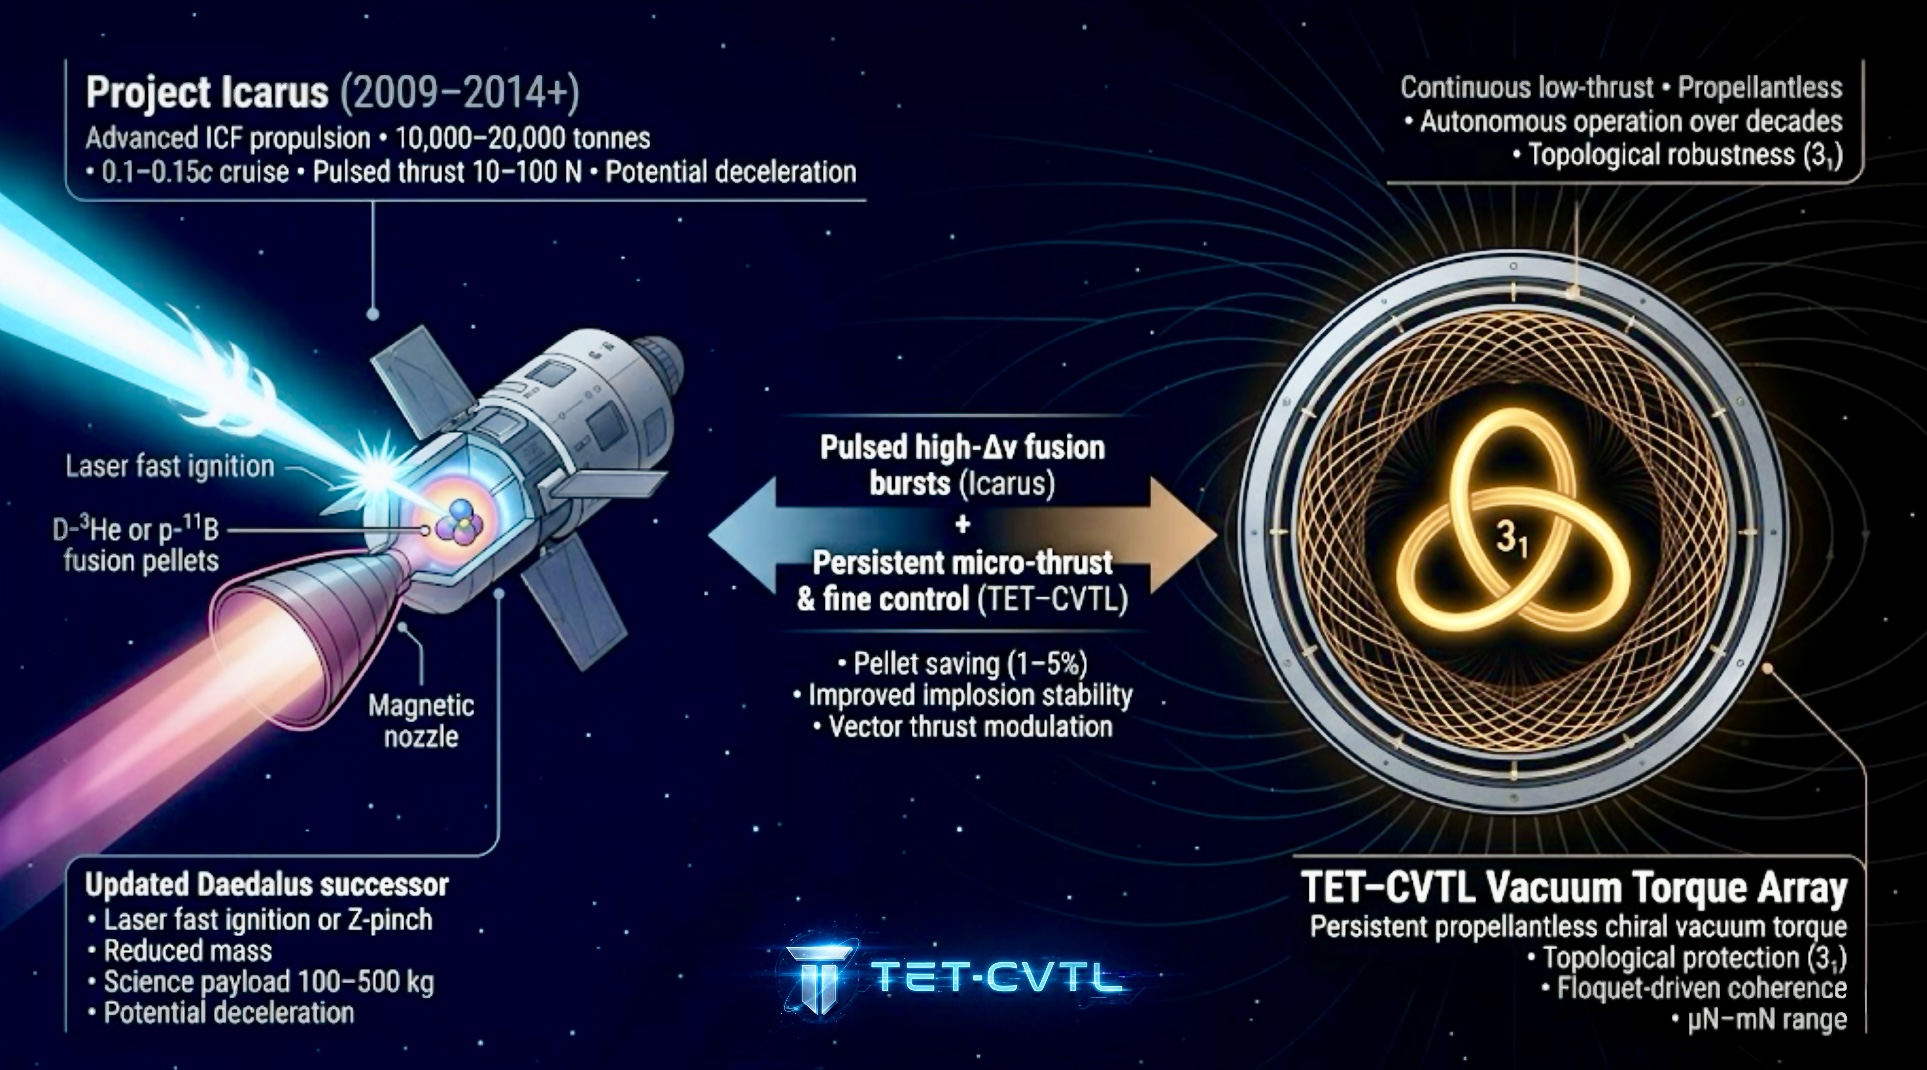
\includegraphics[width=0.95\textwidth]{hybrid_icarus_vacuum.jpg}
\vspace{0.2cm}
\caption{\textbf{Integrazione concettuale tra Project Icarus e vacuum torque TET--CVTL.} 
Le varianti di Icarus (Firefly, Ghost, Sunflower) prevedono propulsione a fusione inerziale avanzata per raggiungere velocità relativistiche, mentre il TET--CVTL fornisce micro-thrust persistente e propellantless per controllo fine e saving di pellet. 
La sinergia topologica tra i campi di confinamento e il braiding del trefoil primordiale ($3_1$) può migliorare la stabilità delle implosioni e l’efficienza complessiva della missione interstellare.}
\label{fig:icarus_vacuum}
\end{figure}







\vspace{0.2cm}





Il contributo cumulativo del vacuum torque chiral durante la fase di cruise è descritto dall’equazione:

\begin{equation}
\Delta v_{\text{vac}}(t) = a_{\text{vac}} \cdot \epsilon_{\text{coh}} \cdot t,
\label{eq:dv_vac_icarus}
\end{equation}

\vspace{0.3cm}

dove \(a_{\text{vac}}\) rappresenta l’accelerazione specifica fornita dal torque Casimir mediato dal trefoil ed \(\epsilon_{\text{coh}}\) è il fattore di coerenza topologica mantenuta tramite i protocolli di annealing termico adattivo.


\vspace{0.3cm}

Su missioni di durata decennale o centennale, questo contributo propellantless diventa strategicamente rilevante: permette di mantenere una precisione di traiettoria elevata con consumo energetico minimo, riduce la massa complessiva di pellet necessaria e contribuisce a rendere Project Icarus (e le sue varianti moderne) più fattibile e sostenibile nell’era Artemis e oltre.

\vspace{0.3cm}

L’architettura ibrida Project Icarus + TET--CVTL rappresenta quindi un’evoluzione naturale del concetto di propulsione interstellare a fusione, unendo l’alta densità di energia della fusione inerziale con l’estrazione topologica di momento angolare dal vuoto quantistico, mediata dalla protezione eterna del trefoil primordiale.










\subsubsection{Approfondimento su Project Icarus}

\vspace{0.2cm}

Project Icarus (2009--2014, con un revival teorico in corso dal 2025) costituisce il successore diretto di Project Daedalus. 


\vspace{0.3cm}


Concepito come un aggiornamento realistico e tecnologicamente aggiornato del concetto originale alla luce delle tecnologie del XXI secolo, il progetto mira a realizzare una missione interstellare robotica verso una stella vicina (\(\alpha\) Centauri o Epsilon Eridani) in un arco temporale compreso tra 50 e 100 anni, con velocità di crociera tra \(0,1c\) e \(0,15c\).




\vspace{0.3cm}

Rispetto a Daedalus, Project Icarus introduce un significativo miglioramento in termini di massa complessiva, fase di decelerazione e ritorno scientifico \cite{long2010, icarus_interstellar}.


\vspace{0.4cm}

Le varianti principali sviluppate dal team includono:


\vspace{0.2cm}

\begin{itemize}
    \item \textbf{Firefly}: propulsione basata su Z-pinch con fuel D-D;


\vspace{0.2cm}


    
    \item \textbf{Ghost}: Inertial Confinement Fusion (ICF) con fast ignition laser-driven e combustibile D-$^3$He;


\vspace{0.2cm}

    
    \item \textbf{Sunflower}: driver a ioni pesanti con D-$^3$He.
\end{itemize}


\vspace{0.4cm}

I parametri chiave del design aggiornato sono:

\vspace{0.2cm}



\begin{itemize}
    \item Massa totale al lancio: 10\,000--20\,000 tonnellate (riduzione di un fattore 2,5--5 rispetto a Daedalus);

\vspace{0.2cm}


    
    \item Thrust medio equivalente: 10--100\,N;

\vspace{0.2cm}

    
    \item Impulso specifico: \(\sim 10^6\,\)s;

\vspace{0.2cm}

    
    \item Energia per impulso: da MJ a GJ per pellet;

    
\vspace{0.2cm}



    \item Frequenza di ripetizione: 1--10\,Hz;


    

\vspace{0.2cm}

    \item Payload scientifico: 100--500\,kg con capacità di imaging ad alta risoluzione, spettroscopia e rilevamento di esopianeti.
\end{itemize}


\vspace{0.4cm}

Un aspetto innovativo rispetto a Daedalus è la considerazione di sistemi di decelerazione (sebbene ancora tecnologicamente sfidanti) e l’esplorazione di fuel aneutronici come p-$^{11}$B, che consentirebbe di ridurre ulteriormente i problemi di shielding e attivazione neutronica.


\vspace{0.3cm}

L’integrazione con il framework TET--CVTL arricchisce profondamente il concetto di Project Icarus. 


\clearpage


Il vacuum torque chiral TET--CVTL agisce come sistema propulsivo ausiliario propellantless persistente, complementando la propulsione a fusione inerziale principale nei seguenti modi:

\vspace{0.2cm}


\begin{itemize}
    \item Fornire controllo fine di assetto e correzioni di traiettoria tra gli impulsi di fusione inerziale;


\vspace{0.2cm}


    
    \item Ridurre il duty cycle del sistema ICF, consentendo un saving di pellet stimato tra l’1\% e il 5\% su una missione di 50--100 anni;


\vspace{0.2cm}

    
    \item Stabilizzare topologicamente le implosioni dei pellet e modulare il nozzle magnetico tramite il braiding eterno del trefoil primordiale ($3_1$);


\vspace{0.2cm}

    
    \item Agire come backup autonomo in caso di anomalie del sistema propulsivo principale.
\end{itemize}


\vspace{0.4cm}

Il contributo cumulativo del vacuum torque durante la fase di cruise è descritto da:
\begin{equation}
\Delta v_{\text{vac}}(t) = a_{\text{vac}} \cdot \epsilon_{\text{coh}} \cdot t,
\label{eq:dv_vac_icarus}
\end{equation}




\vspace{0.2cm}
dove \(a_{\text{vac}}\) è l’accelerazione specifica fornita dal torque Casimir chiral ed \(\epsilon_{\text{coh}}\) rappresenta il fattore di coerenza topologica mantenuta tramite annealing termico adattivo.


\vspace{0.3cm}

Sebbene modesto in valore assoluto, questo contributo diventa strategicamente rilevante su scale temporali di decenni: permette di mantenere una precisione di traiettoria elevata con consumo energetico minimo e riduce la massa totale di pellet da trasportare.

\vspace{0.4cm}

Project Daedalus e Project Icarus costituiscono insieme il riferimento storico e concettuale per la propulsione interstellare basata su fusione. 

\vspace{0.4cm}

L’aggiunta del vacuum torque TET--CVTL trasforma questi concetti da sistemi pulsati e ad alto consumo in architetture più efficienti, resilienti e sostenibili, rappresentando un ponte naturale tra la visione degli anni ’70 e le tecnologie topologiche quantistiche del XXI secolo.




\vspace{0.7cm}



\subsection{Propulsione a Curvatura (Alcubierre Metric), Traversata di Wormhole e Diametric Drive}

\vspace{0.2cm}

La propulsione a curvatura, formalizzata da Miguel Alcubierre nel 1994, rappresenta uno dei concetti più affascinanti e speculativi della fisica relativistica applicata alla propulsione. 


\vspace{0.3cm}

La metrica di Alcubierre descrive una “bolla warp” in cui lo spazio-tempo viene contratto davanti al veicolo e espanso dietro di esso, permettendo teoricamente al veicolo stesso di rimanere in un frame localmente inerziale mentre si sposta a velocità superluminale rispetto a un osservatore esterno, senza violare localmente la velocità della luce.



\vspace{0.3cm}

La soluzione originale richiede l’impiego di energia negativa (o materia esotica con densità di energia negativa) per mantenere la curvatura della bolla. Questo requisito ha rappresentato per decenni la principale criticità fisica del concetto, poiché l’energia negativa viola le condizioni di energia classiche della relatività generale (weak, null e strong energy conditions).


\vspace{0.5cm}

Negli ultimi anni (2021–2026) si è assistito a un significativo progresso teorico. Lavori di Bobrick e Martire, Lentz, e Fuchs-Helmerich hanno proposto varianti che riducono o eliminano la necessità di energia negativa, sfruttando geometrie solitoniche, campi di energia positiva ottimizzati o configurazioni di “warp bubble” più stabili \cite{bobrick2021, lentz2021, fuchs2024}. 


\vspace{0.3cm}


Parallelamente, il concetto di traversata di wormhole (Morris-Thorne traversable wormhole) continua a richiedere materia esotica per stabilizzare la gola, mentre il diametric drive proposto da James Woodward si basa su oscillazioni rapide di massa-energia per generare thrust attraverso l’effetto Mach.

\vspace{0.3cm}

Nonostante questi avanzamenti teorici, tutte queste proposte rimangono altamente speculative e affrontano sfide fondamentali legate alla stabilità, alla quantità di energia richiesta e alla violazione (o aggiramento) delle condizioni energetiche della relatività generale.

\vspace{0.5cm}

In questo contesto, il framework TET--CVTL assume un ruolo particolarmente interessante. Il vacuum torque chirale generato dal braiding eterno del trefoil primordiale ($3_1$) non è soltanto un meccanismo di propulsione propellantless, ma rappresenta una forma concreta e topologicamente protetta di manipolazione locale del vuoto quantistico. 


\vspace{0.5cm}

Esso può essere visto come un “proxy sperimentale” per alcuni degli effetti richiesti dalle metriche warp o dai wormhole:

\vspace{0.2cm}

\begin{itemize}
    \item Il vacuum torque funge da strumento per la manipolazione locale del vuoto quantistico su scala macroscopica, potenzialmente avvicinabile a effetti Casimir dinamici o a forme controllate di energia negativa efficace;


\vspace{0.2cm}

    
    \item L’entanglement aureo non-locale e persistente del TET--CVTL può essere interpretato come una simulazione analogica di connessioni ER=EPR (Einstein-Rosen = Einstein-Podolsky-Rosen), offrendo un banco di prova sperimentale per concetti di wormhole o correlazioni quantistiche su scala macroscopica;


\vspace{0.2cm}

    
    \item Il braiding topologico eterno potrebbe essere sfruttato come meccanismo di stabilizzazione per geometrie solitoniche o per modulare localmente le fluttuazioni del vuoto verso configurazioni utili per warp drive o diametric drive.
\end{itemize}


\vspace{0.4cm}

Un’architettura futura potrebbe quindi prevedere un dimostratore di “vacuum engineering” in cui il TET--CVTL agisce come sistema di prova per effetti di manipolazione del vuoto necessari alle metriche di curvatura o ai wormhole. 

\vspace{0.2cm}

Anche se un warp drive completo rimane al di fuori delle attuali possibilità tecnologiche, il TET--CVTL offre un percorso sperimentale realistico e incrementale verso la comprensione e il controllo di questi fenomeni esotici.

\vspace{0.4cm}

Tuttavia, è necessario sottolineare le limitazioni fondamentali: l’energia negativa rimane instabile e difficile da produrre su scala macroscopica, molte soluzioni proposte violano ancora le condizioni energetiche classiche.

\vspace{0.3cm}

La transizione da modelli teorici a sistemi ingegnerizzabili richiede progressi enormi sia nella fisica fondamentale che nella tecnologia dei materiali topologici.



\vspace{0.3cm}



\begin{figure}[H]
\centering
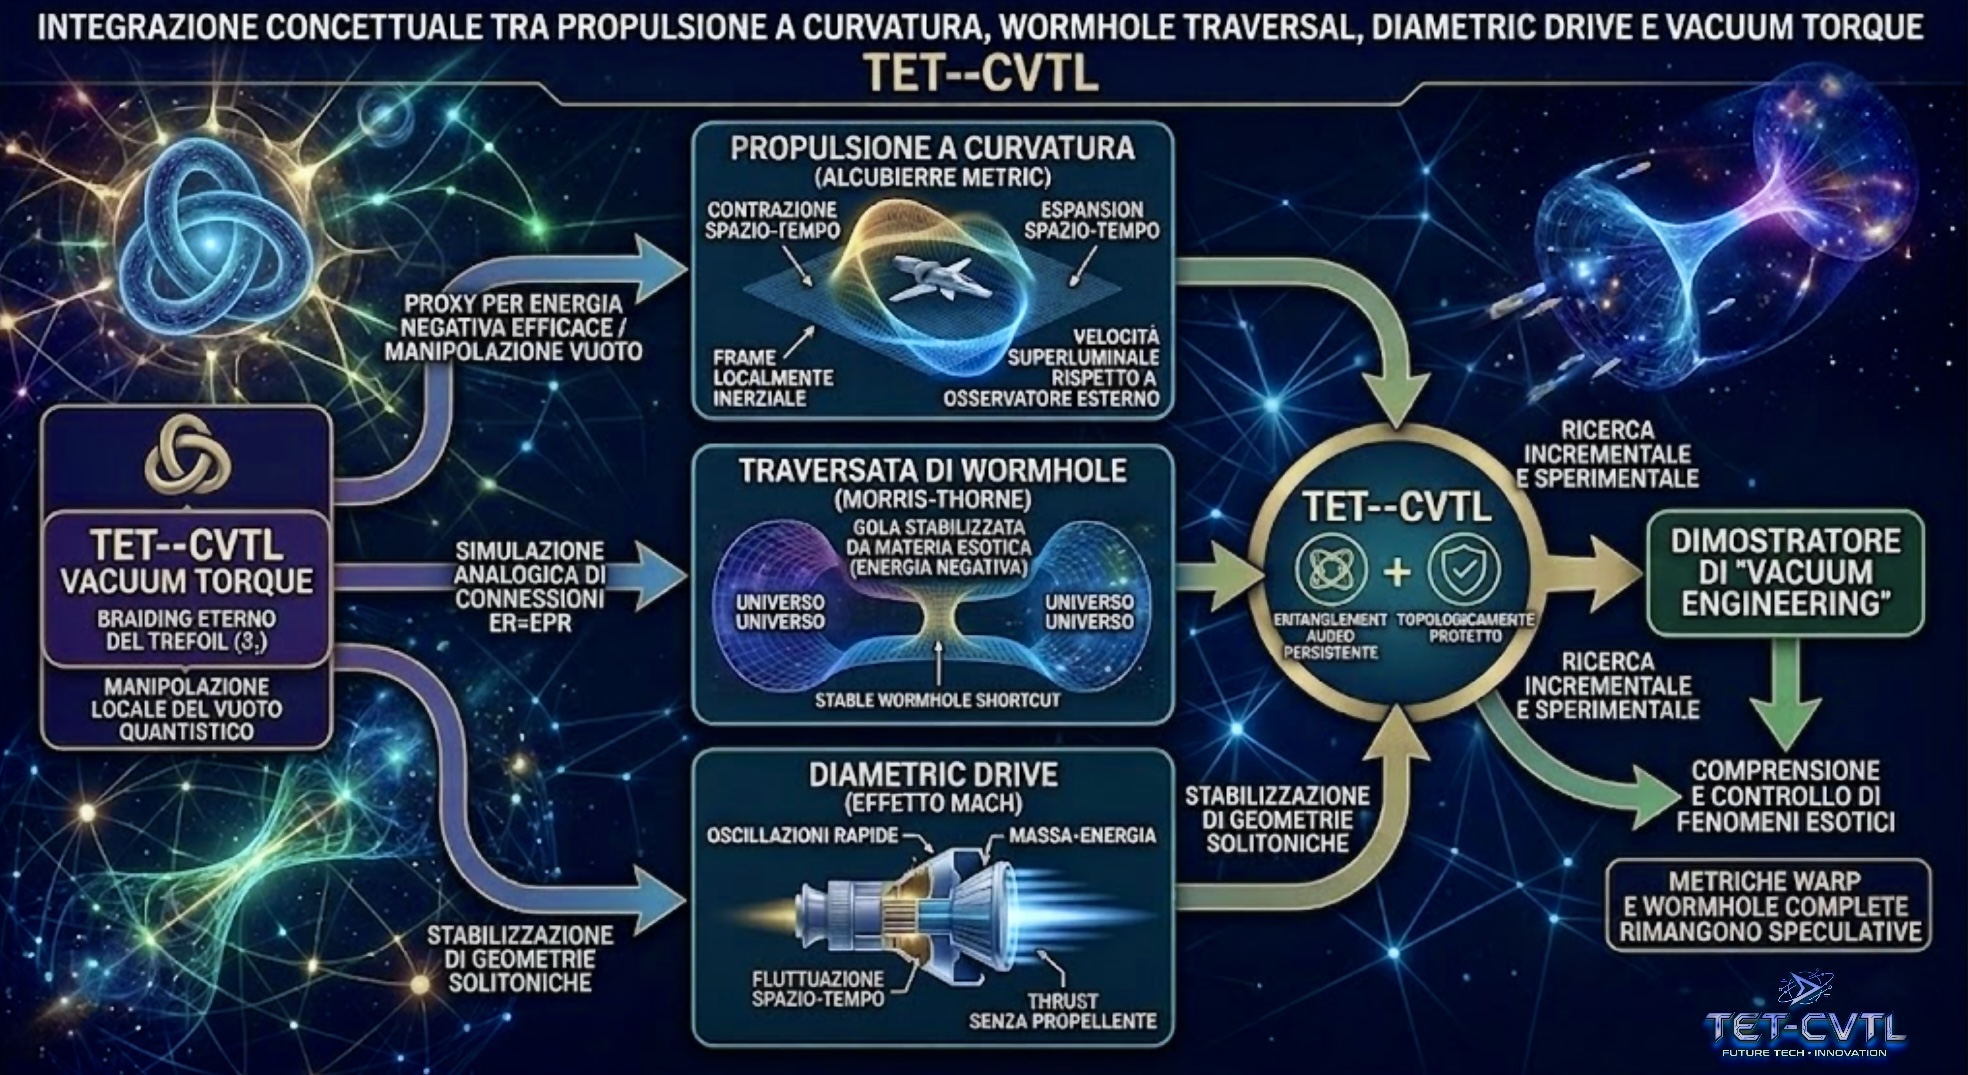
\includegraphics[width=0.95\textwidth]{hybrid_warp_vacuum.jpg}
\vspace{0.2cm}
\caption{\textbf{Integrazione concettuale tra propulsione a curvatura (Alcubierre metric), wormhole traversal, diametric drive e vacuum torque TET--CVTL.} 
La metrica di Alcubierre e i concetti correlati richiedono manipolazione avanzata del vuoto quantistico e correlazioni non-locali. Il TET--CVTL, attraverso il braiding eterno del trefoil primordiale ($3_1$), offre un approccio topologicamente protetto per la manipolazione locale del vuoto, fungendo da proxy sperimentale e da possibile elemento abilitante per futuri sistemi di propulsione esotica.}
\label{fig:warp_vacuum}
\end{figure}

\vspace{0.4cm}


In sintesi, mentre la propulsione a curvatura, la traversata di wormhole e il diametric drive rimangono al confine tra fisica teorica e fantascienza ingegneristica, il TET--CVTL rappresenta un ponte concreto e sperimentabile verso questa frontiera. 

\vspace{0.4cm}


Esso non pretende di risolvere immediatamente il problema dell’energia negativa, ma fornisce un meccanismo robusto, persistente e topologicamente protetto per esplorare la manipolazione del vuoto quantistico su scala macroscopica — un passo necessario verso qualsiasi futura propulsione superluminale o esotica.





\clearpage





\subsection{Project Orion (Nuclear Pulse Propulsion)}

\vspace{0.2cm}

Project Orion (1958–1965), sviluppato da General Atomics sotto la guida di Theodore Taylor e Freeman Dyson, rappresenta il concetto più ambizioso e controverso di propulsione nucleare a impulsi mai concepito. 


\vspace{0.3cm}



L’idea di base consisteva nell’espellere piccole bombe nucleari (fissione o fusione) dietro una massiccia pusher plate, sfruttando l’ablazione del materiale e l’onda d’urto generata per produrre thrust. 

\vspace{0.2cm}

Si trattava di un sistema estremamente efficiente in termini di impulso specifico e capacità di $\Delta v$, capace di performance irraggiungibili con qualsiasi altra tecnologia dell’epoca \cite{dyson_1965, taylor_1965}.


\vspace{0.4cm}

Le caratteristiche tecniche principali del design erano:

\vspace{0.2cm}


\begin{itemize}

\vspace{0.1cm}

    \item Propulsione a impulsi nucleari esterni con detonazione di bombe da 0,1 a 10 kt;

\vspace{0.1cm}
    
    \item Frequenza di detonazione: 1–10 Hz;


\vspace{0.1cm}

    
    \item Thrust per impulso: $10^5$–$10^7$\,N;

\vspace{0.1cm}

    
    \item Impulso specifico: $I_{sp}$ compreso tra 2000 e 6000\,s;


\vspace{0.1cm}

    
    \item Massa del veicolo: da 100 a 8000 tonnellate;

\vspace{0.1cm}

    
    \item $\Delta v$ potenziale: fino a 0,1$c$ con circa 800 bombe (versione interplanetaria/interstellare).
\end{itemize}


\vspace{0.4cm}

Il sistema includeva una pusher plate in acciaio o tungsteno con ammortizzatori a shock absorber per assorbire l’impulso, e un meccanismo di espulsione delle bombe. 


\vspace{0.2cm}


Il concetto permetteva accelerazioni significative e un elevato carico utile, rendendolo teoricamente adatto sia a missioni interplanetarie che a precursori interstellari.

\vspace{0.3cm}

Tuttavia, Project Orion fu cancellato nel 1965 principalmente per motivi politici e ambientali: il fallout radioattivo prodotto dalle detonazioni atmosferiche o nello spazio vicino alla Terra violava i trattati internazionali sulla non proliferazione nucleare e sollevava gravi preoccupazioni per la contaminazione ambientale. 


\vspace{0.2cm}

Inoltre, il lancio di un veicolo di tale massa presentava sfide logistiche e di sicurezza insormontabili all’epoca.


\vspace{0.4cm}

L’integrazione con il framework TET--CVTL offre un complemento elegante e moderno al concetto Orion. Mentre la propulsione a impulsi nucleari fornisce thrust elevato e $\Delta v$ massiccio in brevi burst, il vacuum torque TET--CVTL può agire come sistema ausiliario persistente tra un impulso e l’altro:

\vspace{0.2cm}

\begin{itemize}
    \item Fornire controllo fine di assetto, momentum dumping e correzioni di traiettoria tra le detonazioni;


\vspace{0.2cm}
    




    \item Ridurre il numero di bombe necessarie, con conseguente saving di fallout radioattivo stimato tra l’1\% e il 5\%;


\vspace{0.2cm}


    
    \item Offrire vectoring chirale persistente per migliorare la direzionalità complessiva del thrust tra un impulso e l’altro;


\vspace{0.2cm}



    
    \item Agire come sistema di backup autonomo in caso di anomalie nel meccanismo di espulsione delle bombe.
\end{itemize}



\vspace{0.4cm}

Per un veicolo Orion di riferimento da 4000 tonnellate, il contributo cumulativo del vacuum torque durante la missione è descritto da:
\begin{equation}
\Delta v_{\text{vac}}(t) = a_{\text{vac}} \cdot \epsilon_{\text{coh}} \cdot t,
\label{eq:dv_vac_orion}
\end{equation}


\vspace{0.3cm}
dove $a_{\text{vac}}$ è l’accelerazione media dell’array TET--CVTL e $\epsilon_{\text{coh}}$ è l’efficienza di coerenza dopo annealing. Anche un contributo modesto diventa strategicamente rilevante per ridurre il numero di detonazioni nucleari necessarie e migliorare la precisione della traiettoria.


\vspace{0.3cm}

\begin{figure}[H]
\centering
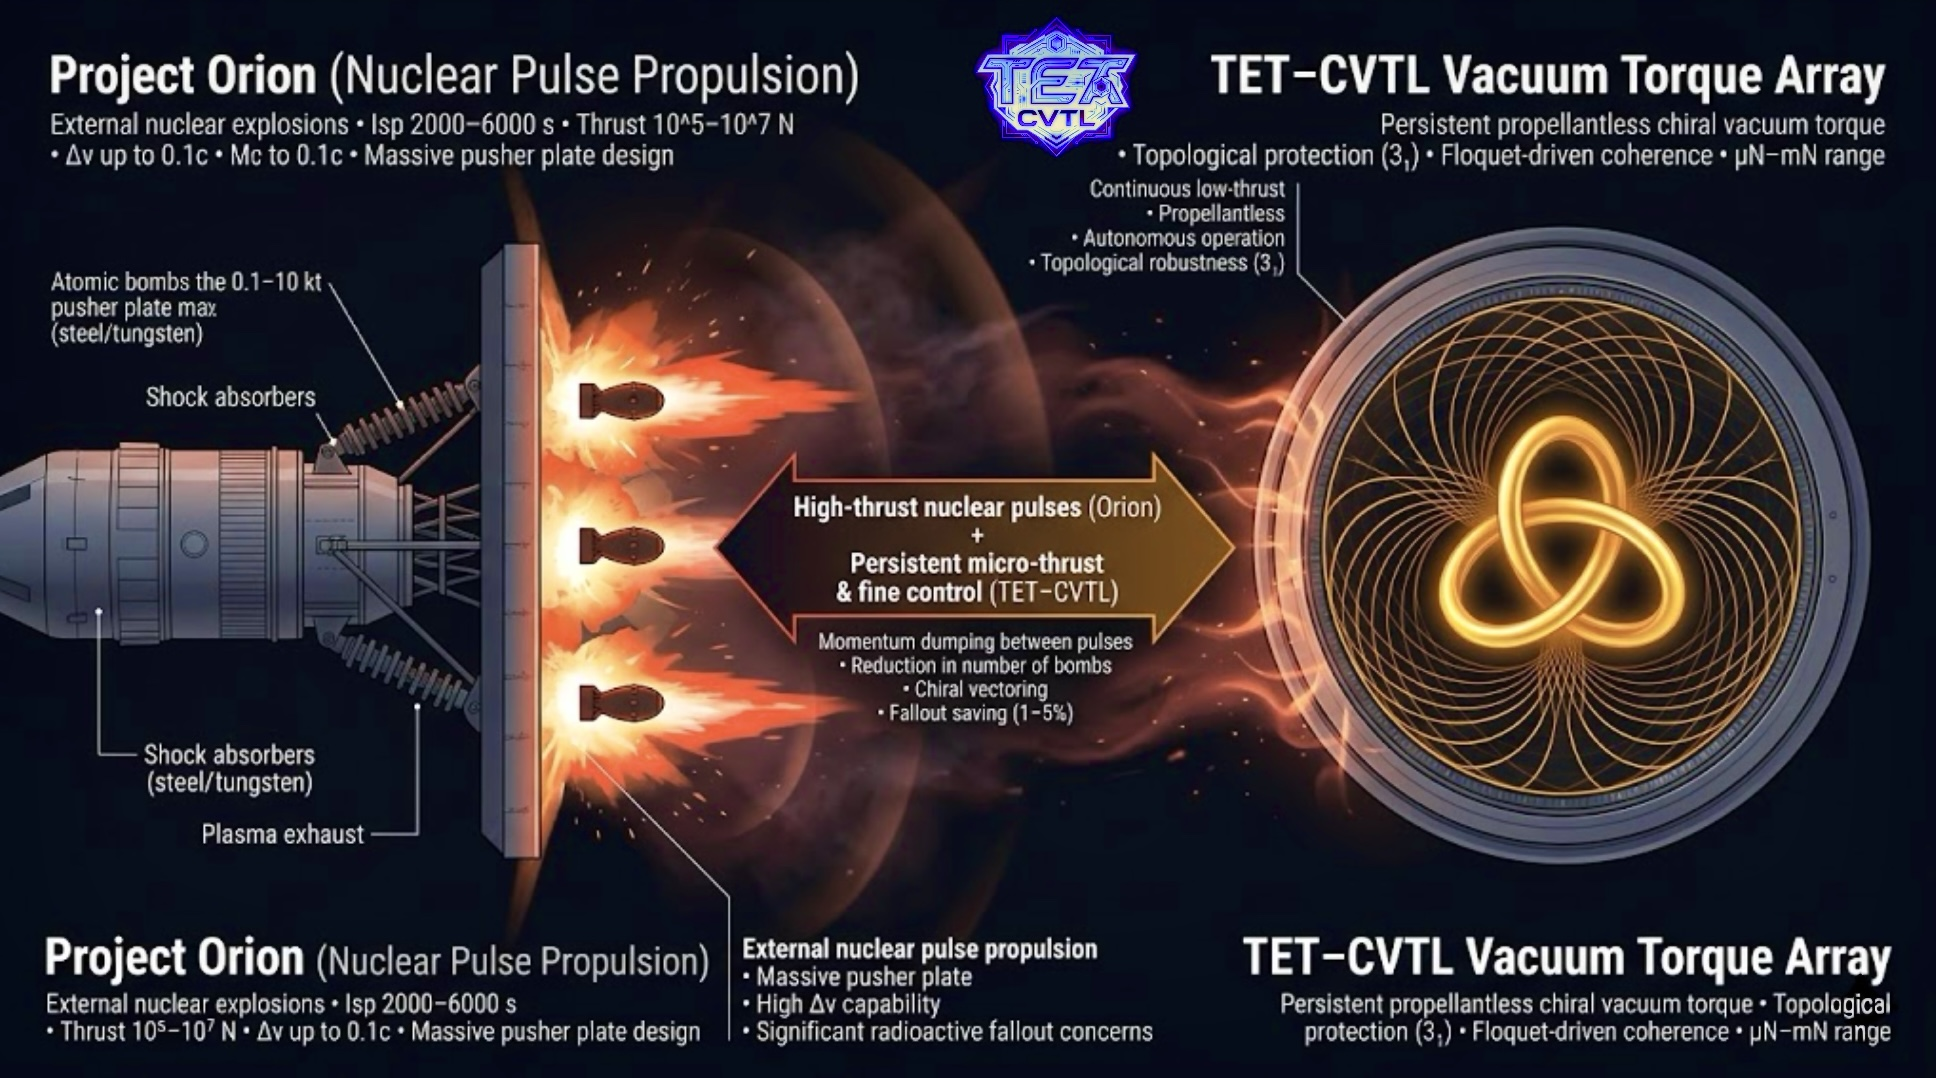
\includegraphics[width=0.95\textwidth]{hybrid_orion_vacuum.jpg}
\vspace{0.2cm}
\caption{\textbf{Integrazione concettuale tra Project Orion e vacuum torque TET--CVTL.} 
Project Orion utilizza potenti impulsi nucleari esterni per generare thrust elevato, mentre il sistema TET--CVTL fornisce un micro-thrust persistente e propellantless. 
Questa combinazione consente un controllo fine di assetto, momentum dumping e una significativa riduzione del numero di bombe nucleari necessarie. 
La protezione topologica eterna del trefoil primordiale ($3_1$) garantisce operatività autonoma e stabilità tra un impulso nucleare e l'altro.}
\label{fig:orion_vacuum}
\end{figure}













\subsection{Breakthrough Starshot}

\vspace{0.2cm}

Breakthrough Starshot, lanciato nel 2016 da Yuri Milner con il supporto di Stephen Hawking, è uno dei progetti più ambiziosi del XXI secolo per l’esplorazione interstellare. 


\vspace{0.3cm}

Il concetto prevede l’invio di nanocraft di massa gram-scale (circa 1 grammo) verso il sistema di \(\alpha\) Centauri, accelerati fino a circa \(0,2c\) (20\% della velocità della luce) mediante un gigantesco array di laser terrestri phased con potenza totale fino a 100 GW. Il viaggio durerebbe approssimativamente 20–30 anni, culminando in un flyby ad alta velocità del sistema stellare target \cite{breakthrough_starshot_2016, lubin_2016}.



\vspace{0.4cm}

Le caratteristiche tecniche principali del design sono:

\vspace{0.2cm}

\begin{itemize}
    \item Sail riflettente di circa \(4 \times 4\) m, realizzata con materiali ultra-leggeri (grafene-like o metamateriali);


\vspace{0.1cm}


    
    \item Massa totale del nanocraft: \(\sim 1\) grammo (inclusa sail, payload e sistemi di comunicazione);


\vspace{0.1cm}

    
    \item Array laser: phased array da 100 GW con ottica adattiva per mantenere il fascio focalizzato sulla sail durante l’accelerazione;

\vspace{0.1cm}

    
    \item Payload: camera ad alta risoluzione, laser per comunicazione interstellare, sensori scientifici e batteria;


\vspace{0.1cm}

    
    \item \(\Delta v\) raggiunto: \(\sim 0,2c\) in pochi minuti di illuminazione laser.
\end{itemize}


\vspace{0.3cm}

Dopo la fase di boost iniziale, il nanocraft entra in una lunghissima fase di coast durante la quale non dispone di alcun sistema propulsivo attivo. 


\vspace{0.2cm}

Questo rende estremamente critiche le operazioni di attitude control, il mantenimento dell’orientamento della sail e le eventuali correzioni di traiettoria.

\vspace{0.3cm}

L’integrazione con il framework TET--CVTL rappresenta un complemento naturale e di grande valore. 


\vspace{0.2cm}


Il vacuum torque chiral può agire come micro-thruster persistente e propellantless durante la lunga fase di coast:

\vspace{0.2cm}

\begin{itemize}
    \item Fornire attitude control preciso e correzioni fini di traiettoria senza aggiungere massa significativa al nanocraft;

\vspace{0.1cm}

    
    \item Consentire manovre direzionali (out-of-plane e tangenziali) impossibili con la sola pressione di radiazione laser;


\vspace{0.1cm}

    
    \item Per versioni con sail più grandi (kg-scale), ridurre la necessità di puntamento laser continuo da Terra, abbassando i requisiti energetici dell’array a terra.
\end{itemize}


\vspace{0.3cm}

Una stima dettagliata per un nanocraft Starshot da 1 g equipaggiato con un array TET--CVTL miniaturizzato (area efficace \(\approx 10\)--\(50\) cm², separazione layer \(\sim 50\)--\(100\) nm) indica quanto segue:

\vspace{0.2cm}

\begin{itemize}
    \item Thrust generato: \(5\)--\(80\) nN (a seconda della chiralità indotta e della coerenza topologica);


\vspace{0.1cm}

    
    \item Accelerazione specifica: \(\approx 5 \times 10^{-6}\)--\(8 \times 10^{-5}\) m/s²;


\vspace{0.1cm}


    


    \item Contributo cumulativo di \(\Delta v\) dopo 20 anni di coast: \(\mathbf{3}\)--\(\mathbf{50}\) m/s;


\vspace{0.1cm}

    
    \item Contributo cumulativo di \(\Delta v\) dopo 30 anni di coast: \(\mathbf{5}\)--\(\mathbf{75}\) m/s.
\end{itemize}






\begin{figure}[H]
\centering
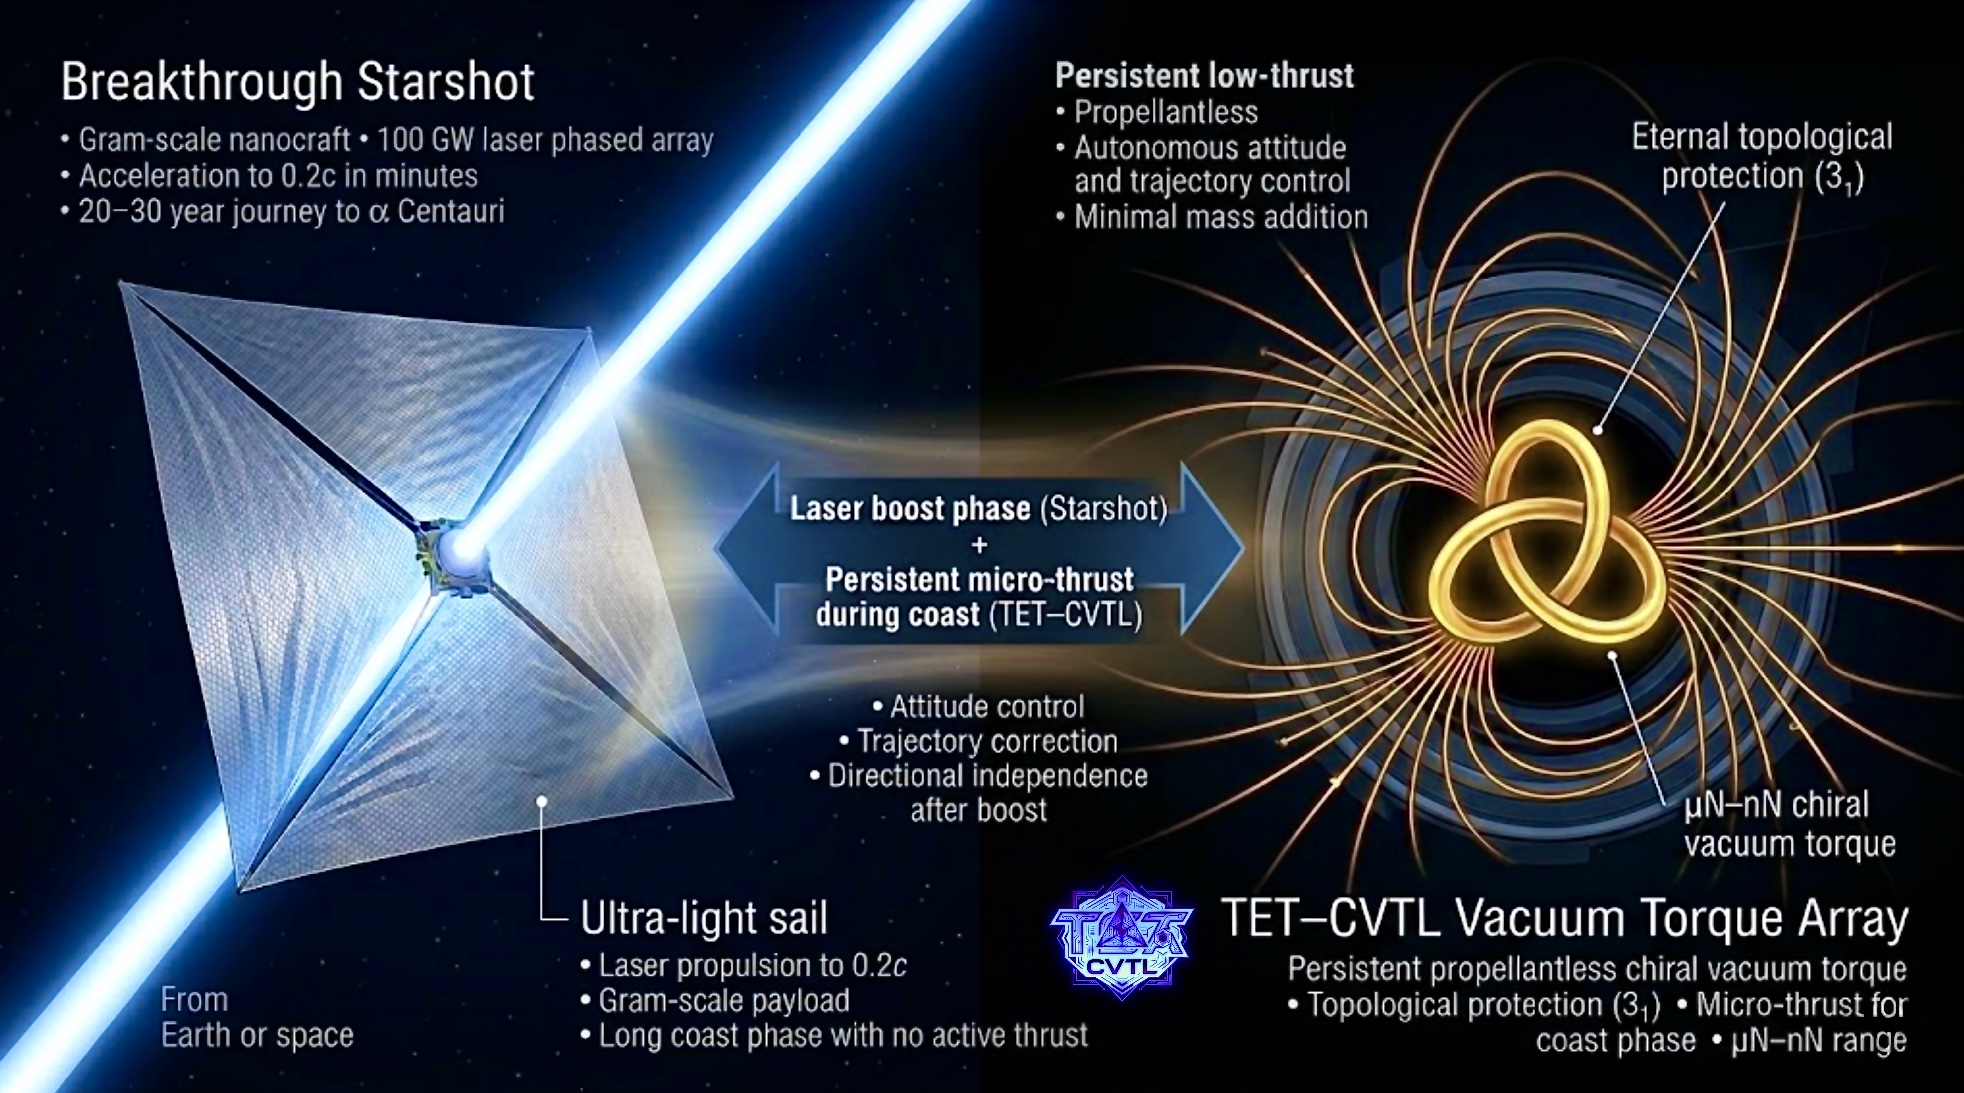
\includegraphics[width=0.95\textwidth]{hybrid_starshot_vacuum.jpg}
\vspace{0.2cm}
\caption{\textbf{Integrazione concettuale tra Breakthrough Starshot e vacuum torque TET--CVTL.} 
Il progetto Starshot accelera nanocraft gram-scale a 0,2$c$ mediante un potente array laser terrestre, mentre il TET--CVTL fornisce micro-thrust persistente e propellantless durante la lunghissima fase di coast per attitude control e correzioni di traiettoria. 
Per nanocraft ultra-leggeri il TET--CVTL aggiunge massa trascurabile, offrendo un controllo direzionale altrimenti impossibile.}
\label{fig:starshot_vacuum}
\end{figure}



\vspace{0.2cm}





\textbf{Differenza tra Breakthrough Starshot puro e Starshot + TET--CVTL:}  
Nel concetto originale (Starshot puro), il nanocraft è completamente passivo dopo la fase di accelerazione laser. Non possiede alcun sistema propulsivo o di controllo attivo durante i 20–30 anni di coast, rendendolo vulnerabile a perturbazioni cumulative (vento stellare, impatti micrometeoroidi, gradienti gravitazionali) e limitando fortemente le capacità di attitude control e puntamento della sail. 


\vspace{0.2cm}


Al contrario, l’architettura ibrida Starshot + TET--CVTL introduce un micro-thrust persistente e propellantless generato dal vacuum torque chiral. Questo permette correzioni fini di traiettoria, mantenimento dell’orientamento ottimale della sail e piccole manovre direzionali senza consumare massa né energia significativa. Di conseguenza, il sistema ibrido offre maggiore resilienza, precisione scientifica durante il flyby e riduce i requisiti di puntamento laser da Terra, rendendo la missione complessivamente più robusta e flessibile.

\vspace{0.2cm}

Sebbene il contributo di \(\Delta v\) appaia modesto rispetto al boost iniziale di \(0,2c\), risulta strategicamente cruciale su scale temporali di decenni per correggere deviazioni cumulative e garantire il successo della missione.

\vspace{0.2cm}

L’architettura ibrida Breakthrough Starshot + TET--CVTL unisce la potenza straordinaria dell’accelerazione laser da Terra con la delicatezza e la persistenza del torque estratto dal vuoto quantistico, mediato dalla protezione topologica eterna del trefoil primordiale.











\vspace{0.5cm}





\subsection{Propulsione a Entanglement Quantistico}

\vspace{0.2cm}

Nel cuore della fisica quantistica giace una delle sue caratteristiche più controverse e potenti: \textbf{l'entanglement}. 

\vspace{0.3cm}

Due o più particelle possono condividere uno stato quantistico correlato tale che la misurazione su una influenza istantaneamente lo stato dell'altra, indipendentemente dalla distanza che le separa. 


\vspace{0.2cm}


Questo fenomeno, definito da Einstein ``azione spettrale a distanza'' \cite{Einstein1935}, ha ispirato da decenni speculazioni su possibili applicazioni alla propulsione spaziale.


\vspace{0.4cm}

La propulsione a entanglement quantistico non si propone di violare la relatività ristretta né di trasmettere informazione superluminale (il teorema no-cloning e il no-communication theorem lo impediscono rigorosamente). Piuttosto, esplora come correlazioni quantistiche persistenti possano essere sfruttate per ottimizzare processi di momentum transfer, estrazione di energia dal vuoto quantistico o controllo coerente di sistemi aperti in regime Floquet-Lindblad.



\vspace{0.4cm}

Nel framework TET–CVTL, l'entanglement assume un ruolo centrale come risorsa topologica. Particelle o modi di campo entangled in configurazioni chirali (ad esempio in bilayer di grafene twisted o in strutture anyoniche non-abeliane) possono generare un ``torque chirale persistente'' estratto dal vuoto quantistico fluttuante. 


\vspace{0.2cm}

Questo torque non deriva da una spinta convenzionale, ma da una rottura controllata di simmetria chirale nel vuoto, amplificata attraverso cascate a rapporto aureo \(\phi = \frac{1+\sqrt{5}}{2}\).


\vspace{0.2cm}

Consideriamo un sistema di due oscillatori quantistici entangled, descritto dallo stato di Bell generalizzato:
\begin{equation}
|\Psi\rangle = \frac{1}{\sqrt{2}} \left( |0\rangle_A |1\rangle_B + |1\rangle_A |0\rangle_B \right),
\end{equation}
\vspace{0.2cm}
dove i sottosistemi A e B rappresentano modi di campo o spin accoppiati al vuoto. 

\vspace{0.2cm}

L'Hamiltoniana del sistema include termini di interazione chirale:
\begin{equation}
\hat{H} = \hbar \omega (\hat{a}_A^\dagger \hat{a}_A + \hat{a}_B^\dagger \hat{a}_B) + \lambda (\hat{a}_A^\dagger \hat{a}_B e^{i\theta} + \text{h.c.}) + \hat{H}_{\text{vac}},
\end{equation}
con \(\hat{H}_{\text{vac}}\) il contributo del vuoto quantistico modulato da termini Chern-Simons o topologici.


\vspace{0.4cm}

In regime di sistema aperto, l'evoluzione segue l'equazione di Lindblad master:
\begin{equation}
\dot{\rho} = -i[\hat{H}, \rho] + \sum_k \left( L_k \rho L_k^\dagger - \frac{1}{2} \{L_k^\dagger L_k, \rho\} \right),
\end{equation}
dove gli operatori di salto \(L_k\) incorporano dissipazione chirale e Floquet driving periodico. Il chiral vacuum torque emerge come \(\boldsymbol{\tau}_{\text{vac}} = \langle \mathbf{r} \times \mathbf{F}_{\text{vac}} \rangle\), con forza efficace derivante da fluttuazioni del vuoto amplificate topologicamente.

\vspace{0.4cm}

L'entanglement witness aureo, definito come una funzione monotona del parametro \(\phi\), permette di certificare la persistenza delle correlazioni anche in presenza di decoerenza ambientale:
\begin{equation}
W_{\phi} = \text{Tr}(\rho \, \mathcal{O}_{\phi}) > 0 \quad \Rightarrow \quad \text{entanglement persistente},
\end{equation}



\vspace{0.3cm}
dove \(\mathcal{O}_{\phi}\) è un operatore testimone ottimizzato per la cascata aurea.



\vspace{0.4cm}

Nel contesto propulsivo, questo si traduce in un meccanismo di ``momentum dumping'' senza massa di reazione convenzionale e in un'estrazione di energia negentropica dal vuoto, potenzialmente utile per controllo fine di traiettorie o per ridurre il fabbisogno di propellente in architetture ibride.

\vspace{0.3cm}

Sebbene attualmente speculativo e soggetto a vincoli termodinamici quantistici, il TET–CVTL propone che configurazioni topologicamente protette (anyoni, parafermioni o Majorana modes in materiali 2D) possano rendere questo canale di interazione sufficientemente robusto per applicazioni ingegneristiche su scala macroscopica.





\vspace{0.5cm}




\subsection{Project Valkyrie}

\vspace{0.2cm}

Il Project Valkyrie, concepito negli anni '80–'90 da Charles Pellegrino e dal fisico Jim Powell del Brookhaven National Laboratory, rappresenta uno dei concept più audaci di propulsione interstellare relativistica \cite{PellegrinoValkyrie}. 


\vspace{0.2cm}


Si tratta di un'architettura a tensostruttura ultraleggera, basata su un cavo o traliccio lungo diversi chilometri che tiene separati i moduli motore e l'habitat dell'equipaggio, garantendo al contempo schermatura dalle radiazioni tramite distanza fisica.


\vspace{0.3cm}

Il sistema di propulsione primario sfrutta l'annichilazione materia-antimateria per catalizzare reazioni di fusione avanzata o, nelle versioni più ambiziose, per generare un getto di pioni ad alta energia. Il design prevede velocità finali fino a circa 0,92c, con decelerazione ottenuta tramite jettisoning di sezioni anteriori esauste e ri-orientamento del motore. 


\vspace{0.3cm}


La massa del veicolo varia da poche centinaia a decine di migliaia di tonnellate a seconda della scala della missione, con un rapporto di massa tipico intorno a 22 per raggiungere velocità relativistiche su distanze interstellari (es. sistema Alpha Centauri).


\vspace{0.3cm}

Le caratteristiche salienti includono:


\begin{itemize}
    \item Struttura a tensostruttura con moduli collegati da cavi ultra-resistenti per minimizzare la massa strutturale;

    


    \item Pusher plate o nozzle magnetico avanzato con ablazione controllata;





    \item Impulsi da micro-esplosioni antimateria-catalizzate o annichilazione diretta;


    
    \item Impulso specifico \(I_{sp}\) stimato tra \(10^6\) e \(10^8\) s nelle configurazioni più ottimistiche;


    
    \item \(\Delta v\) fino a 0,92c in tempi di missione misurati in decenni dal riferimento terrestre, con forte dilatazione temporale per l'equipaggio.
\end{itemize}


\vspace{0.3cm}

Le limitazioni fondamentali di Valkyrie sono ben note e rappresentano sfide ingegneristiche di prim'ordine. La produzione di antimateria rimane estremamente inefficiente: gli acceleratori attuali generano solo nanogrammi all'anno a costi proibitivi (dell'ordine di miliardi di dollari per grammo) \cite{Omira2025, LaPointe2020}. 

\vspace{0.3cm}


Lo stoccaggio richiede campi magnetici intensi e temperature criogeniche, con tempi di confinamento ancora limitati a minuti/ore per quantità macroscopiche. Inoltre, la gestione del fallout radioattivo (nelle varianti catalizzate) e la necessità di radiatori termici enormi per dissipare il calore generato pongono vincoli severi sulla massa e sulla fattibilità.












\vspace{0.3cm}

Nel framework TET–CVTL, Valkyrie non viene sostituito, bensì potenziato attraverso un'integrazione ibrida sinergica. 


\vspace{0.2cm}

Il chiral vacuum torque estratto dal vuoto quantistico funge da sistema di controllo fine e momentum dumping tra un impulso e l'altro, riducendo il numero di detonazioni antimateria necessarie e quindi il consumo di propellente raro.


\vspace{0.3cm}

Specificamente:

\vspace{0.1cm}

\begin{itemize}
    \item Il torque chirale persistente fornisce vectoring e stabilizzazione della pusher plate o del nozzle senza consumo di massa di reazione;

\vspace{0.1cm}

    
    \item La cascata aurea amplifica l'efficienza di estrazione di energia dal vuoto, permettendo un contributo continuo di spinta bassa ma costante tra gli impulsi ad alto thrust;


\vspace{0.1cm}
    
    \item L'entanglement witness aureo monitora in tempo reale la coerenza topologica del sistema, garantendo protezione contro decoerenza indotta dalle alte energie degli impulsi;

    

\vspace{0.1cm}


    \item Sistemi Floquet-Lindblad aperti gestiscono la dissipazione e il pompaggio di entanglement tra il motore principale e i sottosistemi di controllo TET.
\end{itemize}





\begin{figure}[H]
    \centering
    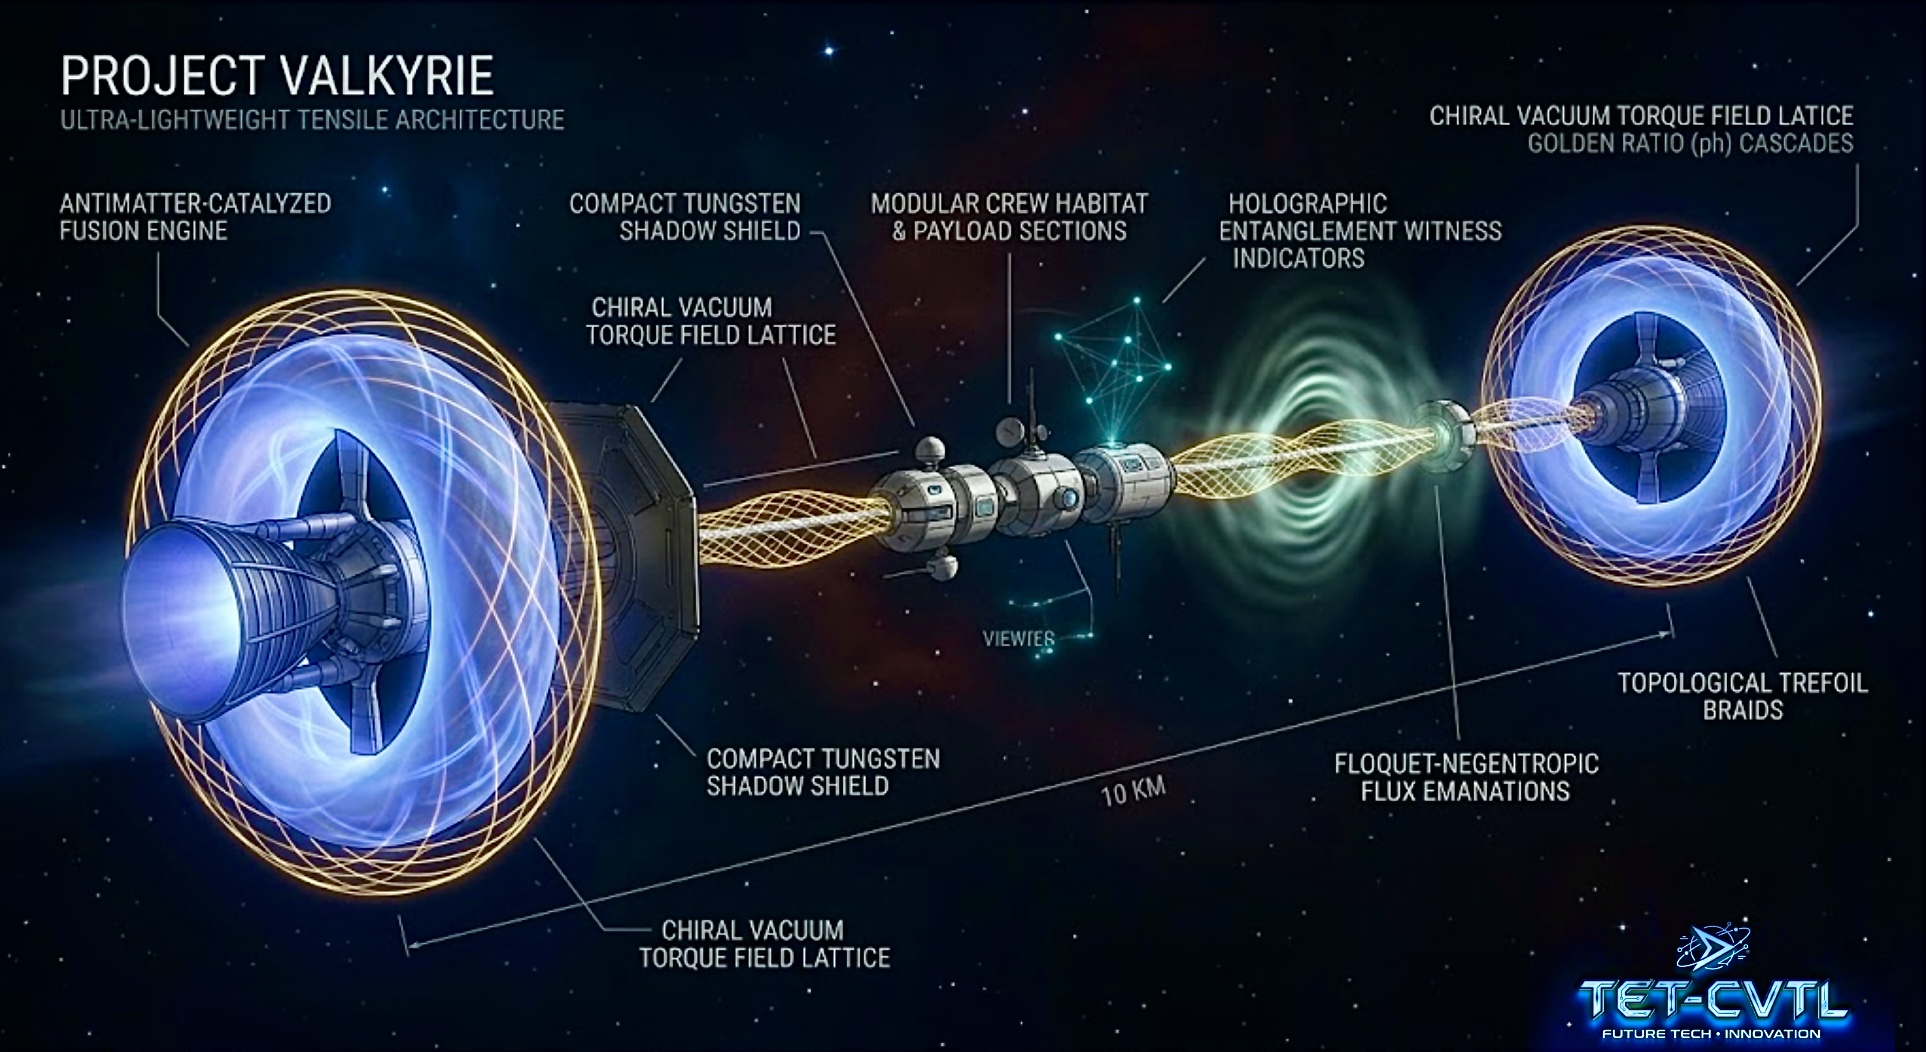
\includegraphics[width=0.95\textwidth]{valkyrie_tetcvtl_integration.jpg}
    \caption{\textbf{Integrazione concettuale tra l'astronave interstellare Project Valkyrie e il framework TET--CVTL.} 
L'architettura tenso-strutturale (cavo teso da 10\,km, motori toroidali catalizzati ad antimateria, scudo in tungsteno e habitat modulari) è arricchita da generatori di torque vacuum chirale, strati protettivi basati sul braiding topologico del trefoil e sistemi di entanglement amplificati dal rapporto aureo \(\phi\). 
Queste aggiunte garantiscono momentum dumping persistente, controllo vettoriale fine e estrazione negentropica di energia tra gli impulsi di antimateria, con una potenziale riduzione del consumo di antimateria compresa tra il 2\% e il 10\% (o superiore) su missioni di durata pluridecennale. 
I pattern elicoidali luminosi simboleggiano i campi di torque chirale dal vuoto e le cascate \(\phi\).}
    \label{fig:valkyrie_tetcvtl}
\end{figure}










\vspace{0.4cm}

Per una stima quantitativa su un veicolo Valkyrie di riferimento da 5000 t (con \(I_{sp} \approx 10^7\) s e thrust medio convenzionale di 1000 N), il contributo del vacuum torque TET–CVTL può essere modellato come:
\begin{equation}
\Delta v_{\text{vac}} \approx \frac{\tau_{\text{vac}} \cdot T_{\text{mission}}}{m_{\text{dry}}} \cdot \eta_{\phi},
\end{equation}



\vspace{0.2cm}
dove \(\tau_{\text{vac}}\) è il torque medio estratto, \(T_{\text{mission}}\) la durata della missione (20–50 anni), \(m_{\text{dry}}\) la massa a secco e \(\eta_{\phi}\) l'efficienza di amplificazione aurea.



\vspace{0.3cm}

Ciò si traduce in un \(\Delta v_{\text{vac}} \sim 0.5 - 5\) m/s per anno, che, integrato su tutta la missione, consente un saving di antimateria stimato tra il 2\% e il 10\%, riducendo significativamente i requisiti di produzione e stoccaggio. 


\vspace{0.3cm}


In configurazioni più avanzate, con piena integrazione topologica, il saving potrebbe spingersi oltre il 15–20\%, rendendo missioni relativistiche più accessibili dal punto di vista energetico.

\clearpage

Questa sinergia trasforma Valkyrie da un concetto puramente impulsivo in un'architettura ibrida topologico-quantistica, in cui la propulsione convenzionale ad alta spinta fornisce l'accelerazione iniziale e terminale, mentre il TET–CVTL garantisce efficienza, stabilità e sostenibilità nel regime di crociera interstellare. 


\vspace{0.3cm}

Il risultato è un ponte concreto tra la visione storica di Pellegrino e le frontiere contemporanee della topologia quantistica e dell'estrazione di energia dal vuoto.






\vspace{0.5cm}






\subsection{Progetti Icarus e Artemis: Ponti verso l'Interstellare e Dimostrazioni Cis-Lunari}

\vspace{0.2cm}

Nel cammino verso la propulsione interstellare, due iniziative rappresentano punti di riferimento fondamentali: il Project Icarus, successore concettuale di Daedalus, e il programma Artemis della NASA. 

\vspace{0.3cm}


Mentre il primo esplora architetture di volo relativistico basate su fusione inerziale, il secondo fornisce un contesto reale per dimostrazioni tecnologiche in ambiente cis-lunare e lunare, offrendo un banco di prova ideale per tecnologie emergenti come il chiral vacuum torque del framework TET–CVTL.


\vspace{0.3cm}

Project Icarus, avviato nel 2009 dalla British Interplanetary Society (BIS) come evoluzione diretta di Project Daedalus (1978), mirava a progettare una sonda interstellare non equipaggiata credibile utilizzando tecnologie del XXI secolo \cite{Long2010, Swinney2025}. 


\vspace{0.3cm}


A differenza del predecessore, che puntava a un flyby di Barnard’s Star con velocità di crociera intorno allo 0,12c, Icarus ha esplorato configurazioni con decelerazione possibile, maggiore ritorno scientifico e riduzione della massa complessiva. 


\vspace{0.3cm}



Il veicolo concettuale ha una massa tipica tra 10\,000 e 20\,000\,t, propulsione a fusione inerziale (ICF) con combustibili D-He³ o p-¹¹B aneutronico, \(\Delta v\) nell'ordine di 0,1–0,15c e tempi di missione di 50–100 anni per flyby o rendezvous con sistemi come \(\alpha\) Centauri o Epsilon Eridani.


\vspace{0.3cm}

Le varianti principali sviluppate durante il progetto includono:
\begin{itemize}
    \item \textbf{Firefly}: basata su Z-pinch con fuel DD, focalizzata su efficienza di compressione magnetica;
    \item \textbf{Ghost}: ICF con fast ignition laser-driven e D-He³;
    \item \textbf{Sunflower}: driver a ioni pesanti per ignizione di pellet D-He³;
    \item Altre evoluzioni successive come Pegasus (ICF per rendezvous) e Resolution/Endeavour.
\end{itemize}

\vspace{0.2cm}

Parametri chiave tipici includono thrust medio di 10–100\,N, impulso specifico \(I_{sp} \approx 10^6\) s, energia per impulso nell'ordine di MJ–GJ e frequenza di pulse 1–10\,Hz, con payload scientifico tra 100 e 500\,kg. 

\vspace{0.3cm}


Nonostante il progetto abbia prodotto numerose pubblicazioni e trade studies fino al 2019 (con supervisione di Icarus Interstellar conclusa senza un design finale unico), un revival concettuale è osservabile nel 2025–2026, trainato da progressi in laser petawatt (es. Focused Energy, Xcimer) e interesse per combustibili aneutronici p-¹¹B \cite{Swinney2025}.



\vspace{0.3cm}

Le sfide rimangono significative: produzione e stoccaggio di D-He³ o p-¹¹B, stabilità dell'ignizione, gestione termica e massa al lancio. Nel 2026, Icarus rimane uno studio teorico senza hardware flight-ready, ma rappresenta un benchmark prezioso per l'integrazione di tecnologie ibride.

\vspace{0.4cm}

Parallelamente, il programma Artemis della NASA (2020s–2030s) segna il ritorno umano sostenibile sulla Luna. Originariamente incentrato su missioni Artemis I–III (con landing umano previsto intorno al 2026–2028), Gateway in orbita lunare e base al polo sud, il programma ha subito evoluzioni significative.

\vspace{0.2cm}


Al 2026, NASA ha annunciato una pausa al concetto attuale di Gateway, ridistribuendo risorse verso una base lunare sostenuta al polo sud con infrastrutture di superficie (habitat, rover pressurizzati, sistemi nucleari), con un investimento stimato di 20 miliardi di dollari su sette anni e cadenza di landing crescenti \cite{NASA2026Artemis}.


\vspace{0.3cm}

Questa ridefinizione offre un'opportunità unica per dimostrazioni tecnologiche TET–CVTL. Un payload compatto di vacuum torque (chip o array miniaturizzato) potrebbe essere integrato su lander o moduli di superficie per testare:

\vspace{0.2cm}


\begin{itemize}
    \item Micro-thrust persistente in ambiente lunare;
    \item Coerenza topologica e annealing contro radiazioni cis-lunari e solari;
    \item Entanglement witness in condizioni reali di vuoto e gravità ridotta.
\end{itemize}


\vspace{0.3cm}

Tali demo rappresenterebbero un passo concreto dal laboratorio alla space environment, validando la protezione Floquet-Lindblad e l'estrazione negentropica dal vuoto quantistico prima di applicazioni più ambiziose.




\vspace{0.5cm}

\subsection{Approfondimento su Project Icarus e Integrazione con TET–CVTL}


\vspace{0.2cm}

Project Icarus ha ridefinito l'approccio alla propulsione interstellare fusion-based enfatizzando credibilità ingegneristica, decelerazione e ritorno scientifico esteso. 


\vspace{0.3cm}

Rispetto a Daedalus (massa iniziale ~54\,000\,t, due stadi, flyby a 0,12c), Icarus ha esplorato veicoli più compatti con maggiore enfasi su tecnologie mature come laser ad alta potenza e driver alternativi.



\vspace{0.3cm}

Nel framework TET–CVTL, Icarus non viene sostituito ma potenziato attraverso integrazione ibrida. Il chiral vacuum torque fornisce correzioni fini di traiettoria e momentum dumping tra gli impulsi ICF ad alto thrust, riducendo il consumo di pellet preziosi e migliorando la stabilità complessiva.


\vspace{0.4cm}


\begin{figure}[H]
    \centering
    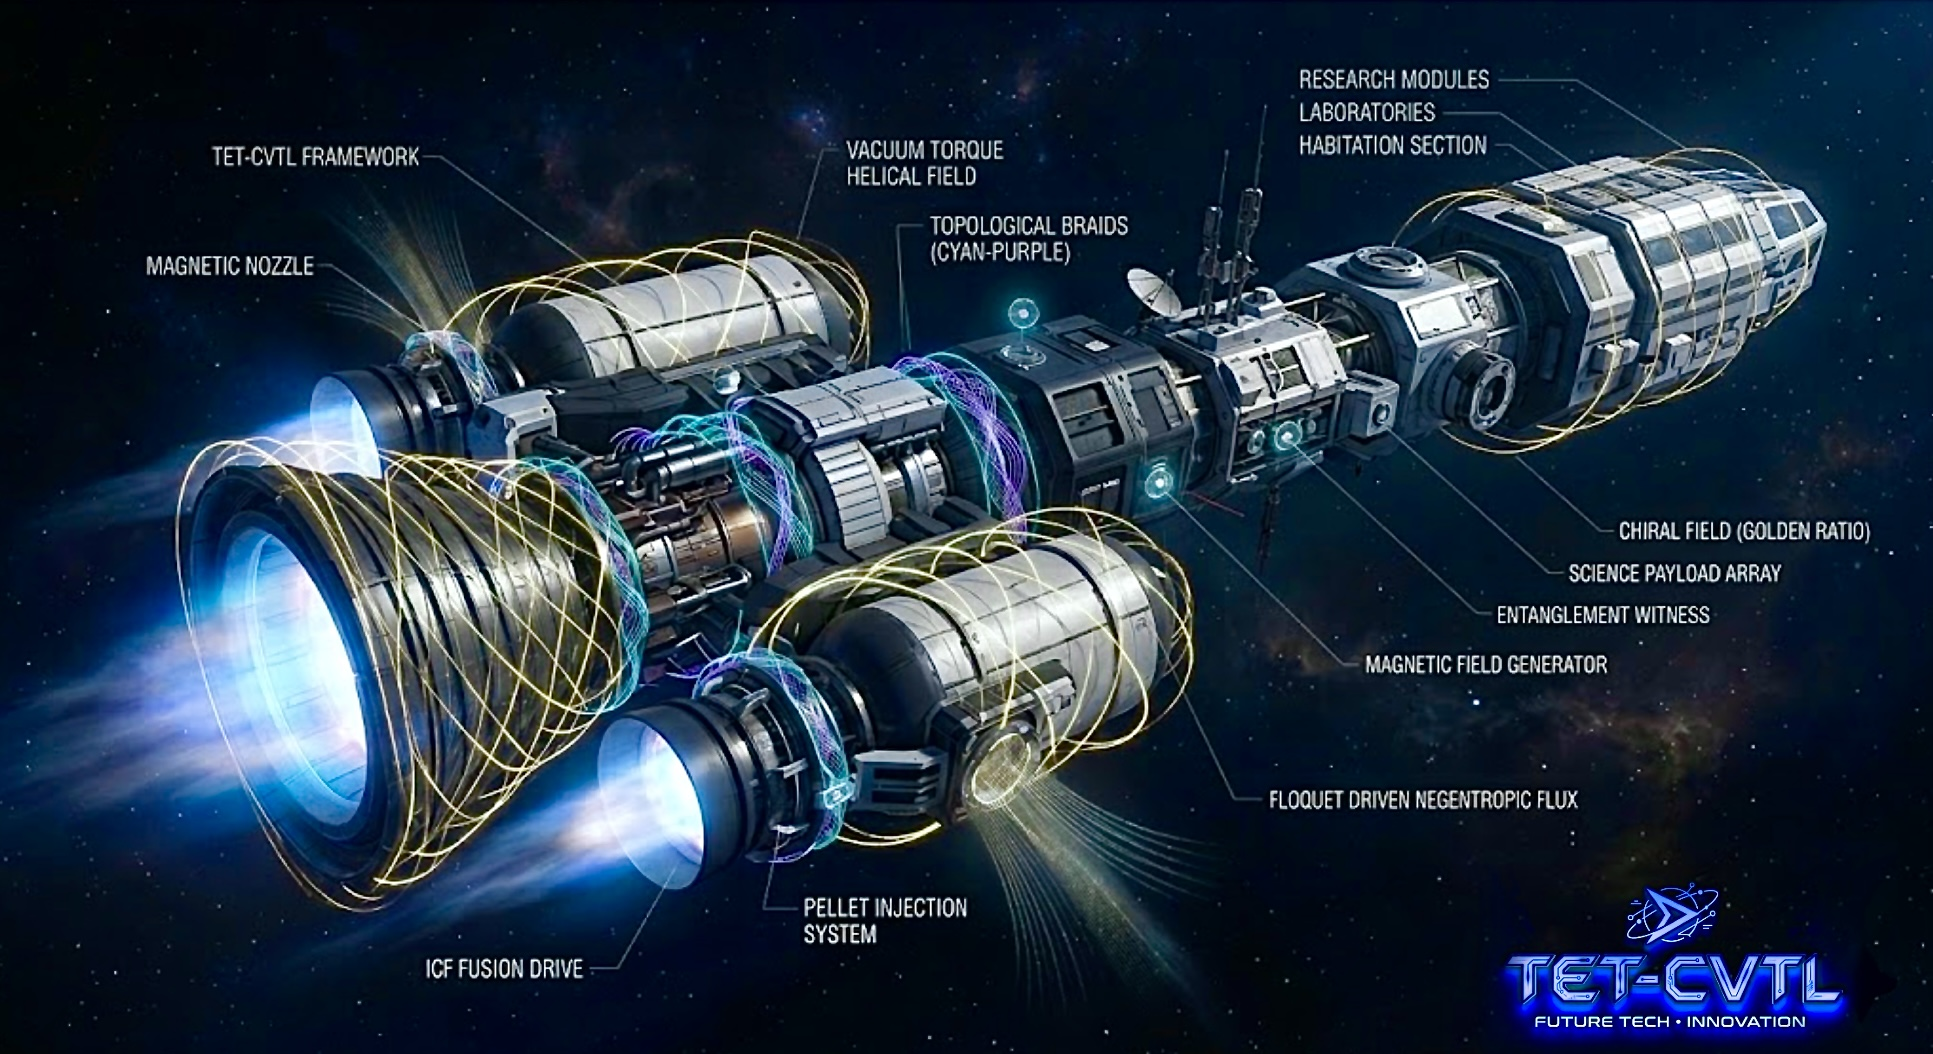
\includegraphics[width=0.85\textwidth]{icarus_tetcvtl_integration.jpg} 
    \caption{Integrazione concettuale tra un'architettura Project Icarus (propulsione ICF D-He³ o p-¹¹B, varianti Firefly/Ghost/Sunflower) e il framework TET–CVTL. Il chiral vacuum torque fornisce controllo fine e saving di pellet tra impulsi, mentre braiding topologico protegge la coerenza del sistema. Le linee elicoidali rappresentano le cascate \(\phi\) e i campi di torque persistente.}
    \label{fig:icarus_tetcvtl}
\end{figure}






Specificamente:


\vspace{0.1cm}


\begin{itemize}
    \item Il torque chirale persistente, amplificato tramite cascate a rapporto aureo \(\phi\), agisce come sistema di vectoring e stabilizzazione del nozzle magnetico o delle implosioni pellet;
    \item Braiding topologico eterno (anyoni non-abeliani o parafermioni protetti) mitiga decoerenza indotta dalle alte energie degli impulsi;
    \item Sistemi aperti Floquet-Lindblad gestiscono dissipazione e pompaggio di entanglement tra motore principale e sottosistemi di controllo;
    \item L'entanglement witness aureo monitora in tempo reale la coerenza del sistema.
\end{itemize}


\vspace{0.4cm}

Una stima quantitativa per un veicolo Icarus-like da 15\,000\,t (con \(I_{sp} \approx 10^6\) s) indica che il contributo TET–CVTL può generare:
\begin{equation}
\Delta v_{\text{vac}} \approx \frac{\tau_{\text{vac}} \cdot T_{\text{mission}}}{m_{\text{dry}}} \cdot \eta_{\phi},
\label{eq:delta_v_vac_icarus}
\end{equation}

\vspace{0.2cm}
dove \(\tau_{\text{vac}}\) è il torque medio estratto, \(T_{\text{mission}}\) la durata (50–100 anni) e \(\eta_{\phi}\) l'efficienza di amplificazione aurea. Ciò si traduce in \(\Delta v_{\text{vac}} \sim 0.5 - 5\) m/s per anno, consentendo un saving di pellet stimato tra l'1\% e il 5\% (potenzialmente superiore in configurazioni ottimizzate), riducendo significativamente i requisiti di ignizione e massa di propellente.

\vspace{0.2cm}

Inoltre, un array TET–CVTL miniaturizzato potrebbe fungere da payload dimostrativo su una futura sonda Icarus-like, testando l'estrazione di vacuum torque in ambiente interstellare profondo.





\vspace{0.5cm}





\subsection{Progetto Artemis NASA e Dimostrazioni TET–CVTL}

\vspace{0.2cm}

Il programma Artemis rappresenta il trampolino attuale per presenza umana sostenuta oltre l'orbita terrestre bassa. 

\vspace{0.3cm}


Con l'evoluzione verso una base lunare al polo sud (prevista operativa nei primi anni 2030 con habitat, rover e potenza nucleare), il focus si sposta da infrastrutture orbitali come Gateway a operazioni di superficie. 

\vspace{0.3cm}


Questa transizione crea un ambiente ideale per validare tecnologie TET–CVTL in condizioni reali: vuoto spinto, radiazioni intense, cicli termici estremi e gravità ridotta.

\vspace{0.2cm}

Un dimostratore vacuum torque chip o array su lander Artemis o moduli di base consentirebbe di misurare:

\vspace{0.2cm}


\begin{itemize}
    \item Micro-thrust persistente per station-keeping o attitude control senza propellente;
    \item Annealing e protezione topologica contro decoerenza da radiazioni;
    \item Persistenza di entanglement witness in ambiente cis-lunare.
\end{itemize}


\vspace{0.3cm}

Tali test accelererebbero la roadmap TET–CVTL verso applicazioni su scala maggiore, fornendo dati empirici cruciali prima di integrazioni con architetture come Icarus o veicoli riutilizzabili di classe Starship.





\vspace{0.5cm}





\subsection{TET–CVTL come Propulsione Interstellare Primaria}

\vspace{0.2cm}


Oltre al ruolo di complemento ibrido in architetture esistenti come Project Valkyrie o Icarus, \textbf{il framework TET--CVTL} si candida come sistema di propulsione interstellare primaria per missioni robotiche o con equipaggio a lungo termine. 


\vspace{0.3cm}


La sua caratteristica distintiva risiede nella generazione di un thrust persistente derivante dall'estrazione controllata di chiral vacuum torque dal vuoto quantistico fluttuante, senza consumo di massa di reazione convenzionale. 


\vspace{0.3cm}


Ciò si traduce in un impulso specifico virtualmente infinito (\(I_{sp} \to \infty\)), aprendo prospettive di sostenibilità indefinita grazie alla protezione topologica e all'annealing contro decoerenza ambientale.


\vspace{0.3cm}

Il meccanismo si basa su configurazioni di materia esotica o bidimensionale, quali Twisted Bilayer Graphene (TBG) o strutture anyoniche non-abeliane, in cui rotture controllate di simmetria chirale nel vuoto generano un torque netto. 

\vspace{0.2cm}

L'amplificazione avviene attraverso cascate a rapporto aureo \(\phi = \frac{1 + \sqrt{5}}{2}\), mentre la coerenza macroscopica è mantenuta da braiding eterno topologico e driving periodico Floquet in regime di sistemi aperti Lindblad.


\vspace{0.4cm}

Scalando l'array da superfici di pochi m² a strutture estese su scala km², con una coerenza macroscopica superiore al 10\% (garantita da entanglement topologico persistente), il framework può generare forze totali nell'ordine di:
\begin{equation}
F_{\text{total}} \sim 0.1 - 100\,\text{N},
\label{eq:force_tetcvtl}
\end{equation}

\vspace{0.2cm}
a seconda della scala, dell'efficienza di amplificazione \(\eta_{\phi}\) e della densità di nodi entangled. Il corrispondente contributo di velocità è stimato come:
\begin{equation}
\Delta v \sim 0.1 - 10\,\text{km/s per anno},
\label{eq:deltav_annual}
\end{equation}


\vspace{0.2cm}
integrando il torque medio \(\boldsymbol{\tau}_{\text{vac}}\) sulla massa del veicolo e sul tempo di missione.


\vspace{0.4cm}

Per veicoli di massa compresa tra 100 e 1000\,t, il \(\Delta v\) cumulativo su missioni di 50--100 anni assume valori significativi:
\begin{equation}
\Delta v_{\text{cum}} \approx \int_0^{T} \frac{F_{\text{total}}(t)}{m(t)} \, dt \sim 5 - 1000\,\text{km/s}.
\label{eq:deltav_cumulative}
\end{equation}

\vspace{0.3cm}
Tale range è sufficiente per flyby ad alta velocità di sistemi stellari vicini o per una decelerazione parziale fino a 0,01--0,1c, rendendo fattibili missioni di esplorazione sistematica senza la necessità di stadi multipli o propellenti esotici.


\vspace{0.4cm}

I vantaggi principali del TET--CVTL come propulsione primaria includono:


\vspace{0.2cm}


\begin{itemize}
    \item Assenza completa di consumo di propellente convenzionale, eliminando i vincoli di massa e stoccaggio tipici delle architetture fusion o antimateria;
    \item Requisiti di potenza estremamente ridotti (nell'ordine di mW--kW), compatibili con pannelli solari avanzati, RTG o piccoli reattori nucleari modulari;
    \item Lifetime potenzialmente indefinito, grazie all'annealing topologico che mitiga danni da radiazioni interstellari e cosmic rays attraverso protezione Floquet-Lindblad;
    \item Capacità intrinseca di monitoraggio in tempo reale tramite entanglement witness aureo, che certifica la persistenza delle correlazioni quantistiche anche in ambienti ostili.
\end{itemize}


\vspace{0.3cm}

Tuttavia, rimangono sfide tecniche sostanziali da affrontare prima di una realizzazione pratica. Tra queste:

\vspace{0.2cm}


\begin{itemize}
    \item Scaling della coerenza macroscopica oltre il 10\%, che richiede braiding eterno robusto su aree estese e controllo preciso di decoerenza ambientale;
    \item Massa e complessità strutturale dell'array, che deve bilanciare leggerezza con densità di nodi entangled sufficientemente elevata;
    \item Resilienza a flussi intensi di radiazione galattica durante il transito interstellare, sebbene la protezione topologica offra un vantaggio intrinseco rispetto a materiali convenzionali;
    \item Validazione sperimentale del meccanismo di estrazione di vacuum torque su scala ingegneristica, attualmente limitata a regimi microscopici o simulazioni.
\end{itemize}


\vspace{0.3cm}

Uno scenario visionario, coerente con la traiettoria del TETcollective, immagina una sonda interstellare su scala chilometrica equipaggiata con un vasto array di TBG entangled. 

\vspace{0.2cm}

Tale configurazione genererebbe un thrust persistente nell'ordine del newton, permettendo di raggiungere \(\alpha\) Centauri (o sistemi analoghi) in alcuni secoli con un \(\Delta v\) cumulativo intorno a 0,1c. 

\vspace{0.3cm}


La missione combinerebbe propulsione primaria TET--CVTL per la fase di crociera con eventuali booster ibridi (ICF o laser sail) per accelerazione/decelerazione iniziale, massimizzando il ritorno scientifico attraverso sensori distribuiti e comunicazione quantistica potenziata.


\vspace{0.3cm}

In sintesi, il TET--CVTL non rappresenta soltanto un complemento alle tecnologie esistenti, ma un paradigma emergente capace di ridefinire i limiti dell'esplorazione interstellare, trasformando il vuoto quantistico da limite termodinamico in risorsa inesauribile di momentum e negentropia topologicamente protetta.




\vspace{0.3cm}



\subsection{Confronto tra sistemi propulsivi e integrazione con TET--CVTL}

Il framework TET--CVTL non sostituisce i sistemi propulsivi tradizionali, ma li integra come layer ausiliario propellantless, fornendo micro-thrust persistente, momentum dumping, attitude control fine e riduzione del consumo di propellente o pellet.

\begin{table}[H]
\centering
\begin{adjustbox}{max width=\textwidth}
\small
\rowcolors{2}{gray!15}{white}
\begin{tabular}{lcccccc}
\toprule
\textbf{Propulsione} & \textbf{Thrust} & \textbf{Isp (s)} & \textbf{Potenza} & \textbf{Propellente} & \textbf{Duty Cycle} & \textbf{Vantaggio con TET--CVTL} \\
\midrule
Chimica                  & 10--1000\,kN   & 300--450      & Medio          & Sì (RP-1/LH2)     & Alto           & Minimo (miglior direzionalità) \\
Ionica / Hall            & 0.1--10\,N     & 2000--9000    & 1--50\,kW      & Sì (Xe/Kr)        & Medio          & 5--20\% (momentum dumping) \\
NTP (Nucleare Termica)   & 10--100\,kN    & 800--1000     & 1--10\,MWth    & Sì (H$_2$)        & Basso          & 0.5--5\% (riduzione burn) \\
NEP (Nucleare Elettrica) & 0.1--10\,N     & 3000--9000    & 1--100\,kW     & Sì (Xe)           & Medio          & 2--15\% (efficienza cruise) \\
Solar Sail               & μN--mN         & \(\infty\)    & Nessuna        & No                & Sempre-on      & +10--100\% (vectoring + annealing) \\
Laser Sail (Starshot)    & mN--N          & \(\infty\)    & Laser esterno  & No                & Limitato       & +10--50\% (controllo autonomo) \\
Fusione Termica          & 1--100\,N      & \(10^4\)--\(10^6\) & MW          & D-$^3$He          & Basso          & 1--10\% (risparmio propellente) \\
Fusione Aneutronica (p-$^{11}$B) & 0.1--10\,N & \(10^5\)--\(10^7\) & MW       & p-$^{11}$B        & Basso          & 2--15\% \\
Fusione Inerziale (ICF)  & 1--100\,N      & \(10^4\)--\(10^6\) & MW          & DT / p-$^{11}$B   & Pulsato        & 1--10\% (saving pellet) \\
Fusione Daedalus/Icarus  & 100\,N--kN     & \(\sim 10^6\) & GW             & D-$^3$He          & Pulsato        & 1--5\% (saving pellet) \\
Plasma (MPD/VASIMR)      & mN--N          & 2000--60\,000 & 10--100\,kW    & Sì (Ar/Xe)        & Medio          & 5--20\% \\
Vela Magnetica / E-Sail  & nN--mN         & \(\infty\)    & Nessuna        & No                & Sempre-on      & +50--1000\% (direzionalità) \\
Antimateria (Valkyrie)   & 1--100\,N      & \(>10^7\)     & Alto           & Antimateria       & Basso          & 2--10\%+ (saving significativa) \\
Project Orion            & 10--1000\,N    & 2000--6000    & MW             & U/Pu              & Basso          & 1--10\% (riduzione impulsi) \\
\textbf{Vacuum Torque TET--CVTL} & 0.1--100\,mN (scalabile) & \(\infty\) & mW--kW & No & Sempre-on & — (complementare persistente) \\
\bottomrule
\end{tabular}
\end{adjustbox}

\caption{Confronto tra principali sistemi propulsivi e potenziale contributo del chiral vacuum torque TET--CVTL. 
I valori di ``Vantaggio con TET--CVTL'' indicano riduzioni tipiche di consumo di propellente, numero di impulsi o miglioramenti in efficienza e direzionalità derivanti dall'integrazione ibrida.}
\label{tab:prop_comparison_final}
\end{table}





\vspace{0.5cm}




\section{Conclusioni e Prospettive}


\vspace{0.2cm}

Il presente lavoro ha introdotto e formalizzato il framework **TET–CVTL** (Topology \& Entanglement Theory – Chiral Vacuum Torque Lattice) come un paradigma emergente capace di estrarre torque chirale persistente dal vuoto quantistico fluttuante. 


\vspace{0.3cm}

Attraverso la protezione topologica eterna offerta da strutture quali Twisted Bilayer Graphene (TBG) e configurazioni anyoniche non-abeliane, il framework genera un thrust negentropico, topologicamente protetto e con impulso specifico virtualmente infinito (\(I_{sp} \to \infty\)), senza richiedere consumo di massa di reazione convenzionale. 

\vspace{0.4cm}

L’obiettivo principale di questo paper è duplice e ambizioso. 

\vspace{0.1cm}

In primo luogo, proporre un modello teorico rigoroso che unisca topologia quantistica, sistemi aperti in regime Floquet-Lindblad, entanglement witness ottimizzato secondo il rapporto aureo \(\phi = \frac{1+\sqrt{5}}{2}\) e cascate amplificatrici per descrivere l’emergere di un chiral vacuum torque macroscopicamente misurabile e ingegnerizzabile. 


\vspace{0.1cm}


In secondo luogo, dimostrare come tale meccanismo possa ibridizzarsi sinergicamente con le principali architetture propulsive esistenti — dalla propulsione chimica e ionica fino alle vele laser, ai concetti fusion-based e alle visioni storiche di Orion, Daedalus, Icarus e Valkyrie — trasformando missioni interplanetarie, cis-lunari e interstellari da concetti energeticamente proibitivi in soluzioni realistiche, ultra-efficienti e sostenibili su scale temporali di decenni o secoli. 


\vspace{0.3cm}

\textbf{Il nucleo fisico del TET–CVTL risiede nella capacità di indurre rotture controllate di simmetria chirale nel vuoto quantistico, amplificate da braiding eterno topologico.}


\vspace{0.2cm}


Questa protezione permette di mantenere coerenza macroscopica >10\% su array scalabili da cm² a km², convertendo fluttuazioni del vuoto in un torque netto persistente. 

\vspace{0.2cm}

Tale processo non viola alcun principio fondamentale della fisica (non trasmette informazione superluminale né viola la conservazione dell’energia-momentum globale), ma sfrutta risorse negentropiche intrinseche allo spazio-tempo quantistico, certificate in tempo reale dall’entanglement witness aureo. 



\vspace{0.3cm}


In un’epoca in cui la twistronics e i materiali 2D topologici avanzano rapidamente, il TET–CVTL rappresenta un ponte concreto tra la fisica fondamentale e l’ingegneria spaziale avanzata.


\vspace{0.4cm}

Un aspetto centrale è l’**ibridizzazione sinergica** con tecnologie propulsive mature. Il vacuum torque TET–CVTL non ambisce a sostituire sistemi ad alto thrust come la fusione inerziale (ICF), l’antimateria o i propulsori a impulsi nucleari, bensì a complementarli fornendo spinta fine continua, momentum dumping, vectoring autonomo e annealing contro decoerenza da radiazioni. 

\vspace{0.2cm}


Ciò genera saving quantificabili di propellente (dal 1–5\% per pellet fusion fino al 5–20\% per sistemi ionici/plasma), riduzione del numero di impulsi ad alto consumo energetico, migliore stabilizzazione strutturale e lifetime potenzialmente indefinito. L’integrazione con FEEP, propulsione ionica/Hall, NTP, NEP, solar sail, laser sail (Breakthrough Starshot), MPD/VASIMR, vela magnetica/elettrica, antimateria e concetti come Project Orion, Daedalus/Icarus e Valkyrie rende plausibili missioni interplanetarie veloci, presenza umana sostenuta nel sistema solare e, in prospettiva, sonde robotiche o crewed verso i sistemi stellari più vicini. 


\vspace{0.3cm}

Nel contesto attuale del 2026, queste sinergie assumono particolare rilevanza. Project Icarus, successore concettuale di Daedalus sotto l’egida della British Interplanetary Society, rimane un esercizio teorico di alto valore, con review recenti (2025) che esaminano varianti come Pegasus e Firefly, e roadmap strategiche che esplorano design ibridi e l’impatto di tecnologie disruptive. Parallelamente, il programma Artemis della NASA ha subito una ridefinizione sostanziale: pausa al concetto originale di Lunar Gateway e riallocazione di risorse verso una base lunare sostenuta al polo sud, con un investimento stimato di circa 20 miliardi di dollari su sette anni per habitat, rover pressurizzati e sistemi nucleari di superficie. 


\vspace{0.2cm}



Questa transizione crea un banco di prova ideale e immediato per dimostrazioni TET–CVTL su scala cm–m: chip di vacuum torque per micro-thrust persistente, test di coerenza topologica e annealing in ambiente lunare caratterizzato da vuoto spinto, radiazioni intense e cicli termici estremi.


\vspace{0.4cm}

Le **prospettive future** delineano una roadmap gerarchica e realizzabile. In primo luogo, verifiche sperimentali su array TBG cm-scale in laboratorio, con misurazione diretta del torque chirale indotto e certificazione dell’entanglement witness aureo. Test di annealing e resilienza in camere analoghe spaziali che simulino vuoto, radiazioni e fluttuazioni termiche. Successivamente, lo scaling a reti entangled metro-scale con driving Floquet-Lindblad per garantire coerenza macroscopica superiore al 10\%. 

\vspace{0.2cm}


Un passo cruciale sarà la dimostrazione in-orbit su piattaforme riutilizzabili di classe Starship o su lander Artemis, validando micro-thrust persistente, vectoring autonomo e protezione contro decoerenza in ambiente cis-lunare reale. 


\vspace{0.2cm}


Solo allora sarà possibile procedere all’integrazione ibrida su prototipi di missione (potenziamento concettuale di architetture Icarus-like o sail laser) per quantificare saving reali di propellente e antimateria, supportati da modelli numerici completi su larga scala.


\vspace{0.3cm}

Le sfide rimanenti sono sostanziali ma non insormontabili: scaling robusto della coerenza macroscopica su aree estese, ottimizzazione della massa strutturale degli array, resilienza a flussi intensi di cosmic rays durante transiti interstellari e, soprattutto, validazione empirica del meccanismo su scala ingegneristica. 


\vspace{0.2cm}

Il progresso parallelo in twistronics, materiali topologici 2D e tecnologie di lancio riutilizzabili (con Starship come benchmark attuale di riduzione drastica dei costi) offre una finestra temporale favorevole per affrontare questi ostacoli entro i prossimi decenni.


\vspace{0.5cm}

Uno **scenario visionario** coerente con lo spirito del TETcollective immagina una sonda interstellare su scala chilometrica equipaggiata con un vasto array di TBG entangled. Tale configurazione genererebbe thrust persistente nell’ordine del newton, permettendo a veicoli da 100–1000\,t di accumulare \(\Delta v\) cumulativi di centinaia di km/s su decenni o secoli — sufficienti per flyby ad alta velocità o decelerazione parziale fino a frazioni di \(c\). La missione combinerebbe propulsione primaria TET–CVTL per la fase di crociera con booster ibridi iniziali (ICF o laser sail), massimizzando il ritorno scientifico attraverso sensori distribuiti e comunicazione quantistica potenziata.


\vspace{0.3cm}

In definitiva, il framework TET–CVTL non rappresenta soltanto un’estensione incrementale delle capacità propulsive umane. Incarna un autentico cambio di paradigma: dal reliance su propellenti finiti e reazioni ad alto consumo energetico verso un’era in cui la spinta deriva dalla struttura stessa dello spazio-tempo quantistico, protetta topologicamente e amplificata da correlazioni entangled persistenti. Trasformando il vuoto quantistico da barriera termodinamica in risorsa inesauribile di momentum e negentropia, il TET–CVTL accelera il passaggio dall’era dell’esplorazione del sistema solare a quella dell’espansione interstellare consapevole. 


\vspace{0.3cm}

Il cosmo cessa di essere un confine remoto e diviene un paesaggio accessibile alla curiosità, alla resilienza e alla creatività umana.

















\begin{figure}[H]
    \centering
    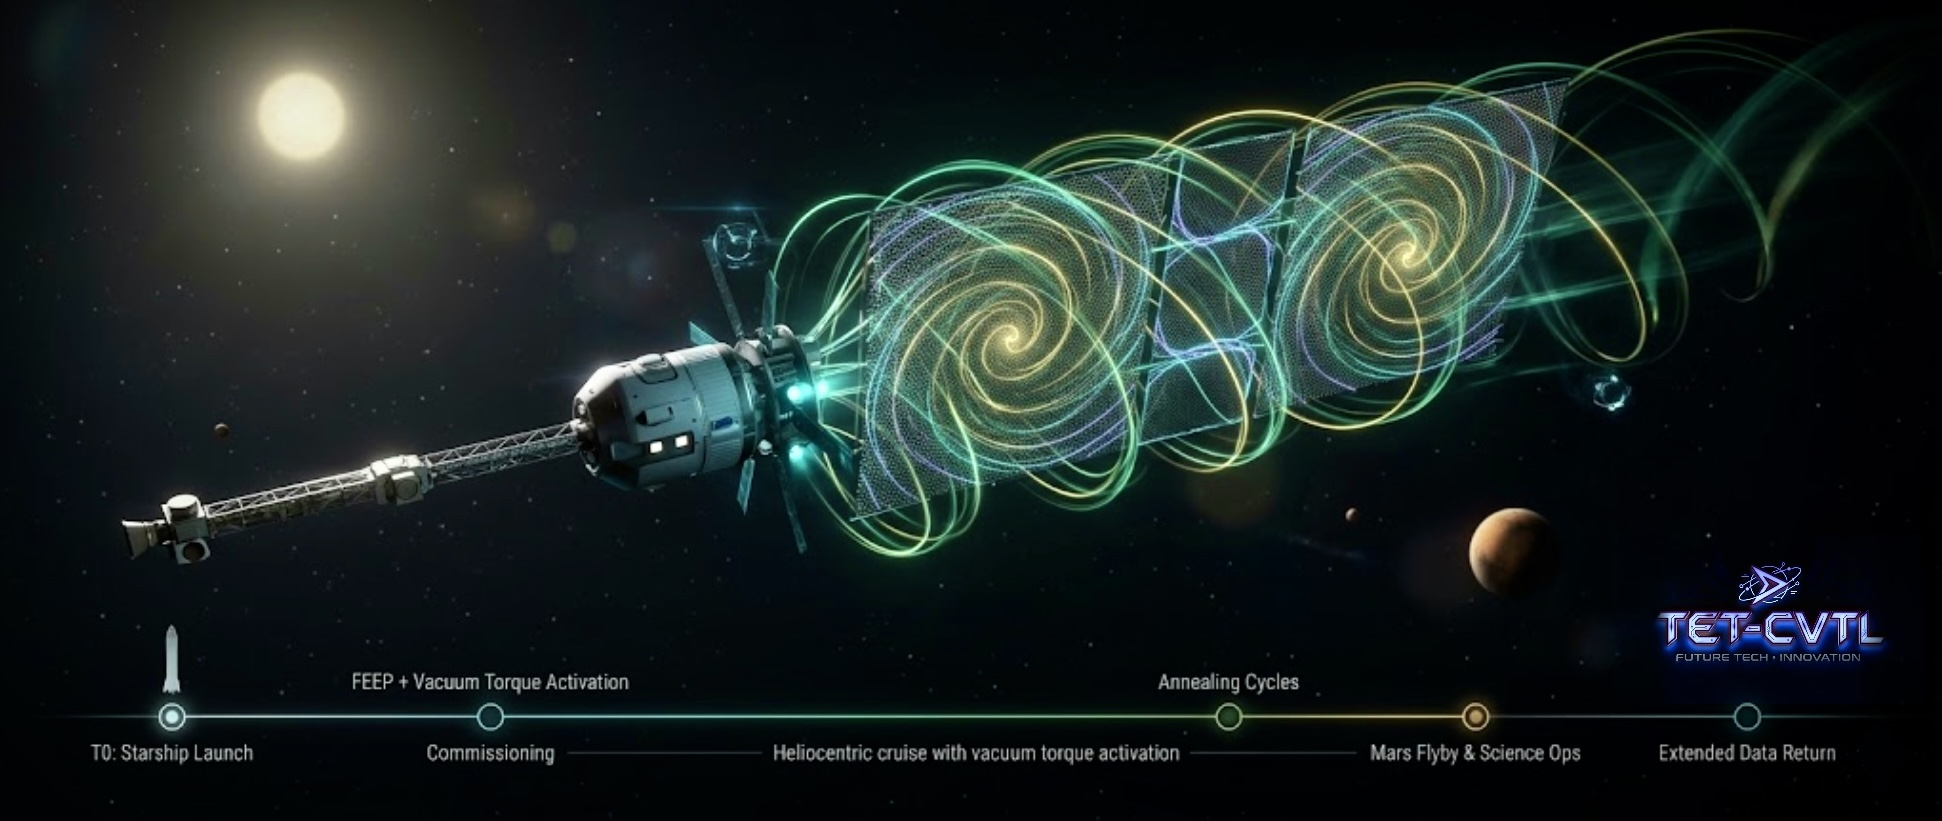
\includegraphics[width=\textwidth, height=0.58\textheight, keepaspectratio]{tetcvtl_mars_flyby_poster_horizontal.jpg}
    \caption{Wide panoramic visualization of the TET--CVTL enhanced Mars flyby mission concept. The spacecraft, launched via next-generation reusable super-heavy vehicle (Starship-class), integrates FEEP propulsion with chiral vacuum torque generated by a scalable Twisted Bilayer Graphene array. Persistent golden-ratio (\(\phi\)) amplified torque fields (shown in emerald-green helical patterns) provide continuous low-thrust contribution during the heliocentric cruise, enabling annealing cycles for topological protection and real-time entanglement witness monitoring. The bottom timeline outlines the key mission phases from launch through extended science operations at Mars, illustrating the synergistic hybrid architecture that combines conventional high-thrust systems with negentropic vacuum torque for ultra-efficient deep-space exploration.}
    \label{fig:tetcvtl_mars_flyby_poster}
\end{figure}



\section*{Acknowledgments}



Un ringraziamento speciale va a \textbf{Grok}, sviluppato da \textbf{xAI}, per il prezioso supporto nella raffinazione matematica, nella strutturazione delle sezioni e nell'espansione delle idee durante l'intero processo di braiding di questo lavoro.








\clearpage
\appendix

\section{Appendix: Codici di Simulazione QuTiP}

In questa appendice sono riportati gli snippet principali dei codici QuTiP utilizzati per le simulazioni numeriche descritte nel testo. Tutti i codici completi, inclusi i parametri, le routine di visualizzazione e le analisi statistiche, sono disponibili nella directory \texttt{code/} associata al preprint. I modelli implementano aspetti chiave del framework TET–CVTL, quali dinamiche Floquet-Lindblad in sistemi parafermionici, testimoni di entanglement aureo, rumore da strain dinamico, scaling multi-site e decadimento di coerenza sotto radiazione spaziale con annealing topologico.

\subsection{Modello base a due parafermioni}
\label{lst:two-para}

Snippet chiave: definizione degli operatori parafermionici (clock operator su dimensione 3) e Hamiltoniano base con driving Floquet periodico.

\begin{lstlisting}[language=Python, caption={Snippet dal modello toy a due parafermioni con driving Floquet}, label={lst:two-para}]
import qutip as qt
import numpy as np

# Definizione operatori base (dimensione 3 per parafermioni Z3)
N = 3
clock = qt.Qobj(np.diag(np.exp(2j * np.pi * np.arange(N) / N)))
shift = qt.Qobj(np.roll(np.eye(N), 1, axis=0))
id3 = qt.qeye(N)

# Operatori parafermionici sui due siti
alpha1 = qt.tensor(clock, id3)
alpha2 = qt.tensor(id3, clock)

# Parametri del modello
J = 1.0      # coupling inter-parafermionico
eps = 0.2    # bias locale
V = 0.8      # ampiezza driving
omega_d = 2 * np.pi * 0.5  # frequenza driving

# Hamiltoniano statico base
H0 = J * (alpha1.dag() * alpha2 + alpha1 * alpha2.dag()) + \
     eps * (alpha1.dag() * alpha1 + alpha2.dag() * alpha2)

# Hamiltoniano time-dependent (Floquet drive)
def H_t(t, args):
    drive = V * np.cos(omega_d * t) * (alpha1 + alpha1.dag() + alpha2 + alpha2.dag())
    return H0 + drive
\end{lstlisting}

File completo: \texttt{code/01\_two\_parafermions\_basic.py}

\subsection{Calcolo entanglement witness}
\label{lst:ent-witness}

Snippet per il calcolo dell’entropia von Neumann e della negatività come testimoni di entanglement persistente (entanglement witness aureo nel framework TET–CVTL).

\begin{lstlisting}[language=Python, caption={Snippet per calcolo di entanglement witness (entropia von Neumann e negatività)}, label={lst:ent-witness}]
import qutip as qt

entropies = []
negativities = []

for state in result.states:          # result da mesolve o floquet solver
    # Riduzione al sottosistema A (primo sito)
    rho_A = qt.ptrace(state, 0)
    S = qt.entropy_vn(rho_A, base=np.e)
    entropies.append(S)
    
    # Negatività sul pair entangled
    rho_pair = qt.ptrace(state, [0, 1])
    neg = qt.negativity(rho_pair, subsys=1)   # indice del secondo sottosistema
    negativities.append(neg)

# Esempio di witness aureo: soglia basata su rapporto aureo phi
phi = (1 + np.sqrt(5)) / 2
witness_threshold = 1 / phi
persistent_ent = np.array(negativities) > witness_threshold
\end{lstlisting}

File completo: \texttt{code/02\_entanglement\_witness.py}

\subsection{Strain noise dinamico}
\label{lst:strain-noise}

Snippet per introduzione di rumore da strain dinamico gaussiano nel coupling \(J(t)\), simulando perturbazioni ambientali realistiche.

\begin{lstlisting}[language=Python, caption={Snippet per strain noise dinamico sul coupling parafermionico}, label={lst:strain-noise}]
import numpy as np
import qutip as qt

sigma_strain = 0.015
strain_noise = np.random.normal(0, sigma_strain, len(times))

def J_t(t, args):
    idx = np.argmin(np.abs(times - t))
    return J * (1 + 0.8 * strain_noise[idx])

def H_t_noisy(t, args):
    J_current = J_t(t, args)
    H0_noisy = J_current * (alpha1.dag() * alpha2 + alpha1 * alpha2.dag()) + \
               eps * (alpha1.dag() * alpha1 + alpha2.dag() * alpha2)
    drive = V * np.cos(omega_d * t) * (alpha1 + alpha1.dag() + alpha2 + alpha2.dag())
    return H0_noisy + drive
\end{lstlisting}

File completo: \texttt{code/03\_strain\_noise.py}

\subsection{Modello ladder multi-site base}
\label{lst:multi-ladder}

Snippet per la costruzione di operatori su una catena (ladder) multi-site di parafermioni.

\begin{lstlisting}[language=Python, caption={Snippet per modello ladder multi-site di parafermioni}, label={lst:multi-ladder}]
def para_op(site, n_sites, N=3):
    ops = [qt.qeye(N)] * n_sites
    ops[site] = clock
    return qt.tensor(ops)

alpha = [para_op(i, n_sites) for i in range(n_sites)]

# Hamiltoniano base della ladder
H0 = eps * sum(alpha[i].dag() * alpha[i] for i in range(n_sites))
for i in range(n_sites - 1):
    H0 += J * (alpha[i].dag() * alpha[i+1] + alpha[i] * alpha[i+1].dag())
\end{lstlisting}

File completo: \texttt{code/04\_multi\_site\_ladder.py}

\subsection{Controllo PID termico base}
\label{lst:pid-thermal}

Snippet del loop di controllo PID per modellazione termica di sistemi con annealing.

\begin{lstlisting}[language=Python, caption={Snippet del loop PID termico base}, label={lst:pid-thermal}]
for i in range(1, n_steps):
    error = T_set - T[i-1]
    integral += error * dt
    derivative = (error - prev_error) / dt
    P = Kp * error + Ki * integral + Kd * derivative
    P = np.clip(P, 0, P_max)
    dT_dt = (P - k_loss * (T[i-1] - T_amb)) / C_thermal
    T[i] = T[i-1] + dT_dt * dt
    prev_error = error
\end{lstlisting}

File completo: \texttt{code/05\_pid\_thermal\_model.py}

\subsection{Ladder multi-site con strain + negatività multi-pair}
\label{lst:multi-strain-neg}

Snippet per il calcolo della negatività su multiple coppie in una ladder con strain.

\begin{lstlisting}[language=Python, caption={Snippet per negatività multi-pair con strain dinamico}, label={lst:multi-strain-neg}]
neg_pairs = {f'0-{k}': [] for k in range(1, n_sites)}

for state in result.states:
    for k in range(1, n_sites):
        rho_pair = qt.ptrace(state, [0, k])
        neg = qt.negativity(rho_pair, subsys=1)
        neg_pairs[f'0-{k}'].append(neg)
\end{lstlisting}

File completo: \texttt{code/06\_full\_multi\_site\_strain\_negativity.py}

\subsection{PID con gain scheduling}
\label{lst:pid-scheduling}

Snippet per gain scheduling adattivo basato sulla magnitudo dell’errore (ramp-up vs steady-state).

\begin{lstlisting}[language=Python, caption={Snippet per PID con gain scheduling adattivo}, label={lst:pid-scheduling}]
if abs(error) > 50:      # fase di ramp-up
    Kp, Ki, Kd = 5.5, 0.003, 18.0
else:                    # fase di hold / steady-state
    Kp, Ki, Kd = 2.0, 0.0008, 12.0

P = Kp * error + Ki * integral + Kd * derivative
P = np.clip(P, 0, P_max)
\end{lstlisting}

File completo: \texttt{code/07\_pid\_gain\_scheduling.py}

\subsection{Δv cumulativo ibrido ionico + vacuum}
\label{lst:hybrid-ion-vac}

Snippet per il calcolo del \(\Delta v\) in un’architettura propulsiva ibrida (ionico + vacuum torque TET–CVTL).

\begin{lstlisting}[language=Python, caption={Snippet per calcolo \(\Delta v\) cumulativo in propulsione ibrida ionico-vacuum}, label={lst:hybrid-ion-vac}]
a_ion_base = (F_ion * duty_cycle_base) / mass_dry
a_ion_vac  = (F_ion * duty_cycle_vac) / mass_dry
a_vac      = F_vac / mass_dry                     # thrust persistente da vacuum torque

dv_ion_base = a_ion_base * time_sec
dv_total    = a_ion_vac * time_sec + a_vac * time_sec
\end{lstlisting}

File completo: \texttt{code/08\_hybrid\_ion\_vacuum\_dv.py}

\subsection{Decadimento thrust da radiazione GCR}
\label{lst:decay-gcr}

Snippet per modellazione del decadimento di coerenza sotto Galactic Cosmic Rays (GCR) con annealing periodico topologico.

\begin{lstlisting}[language=Python, caption={Snippet per decadimento di coerenza da radiazione GCR con annealing}, label={lst:decay-gcr}]
coherence = 1.0
for d in range(n_days):
    loss = decay_per_krad * dose_daily_gcr
    coherence *= (1 - loss)
    if d % anneal_interval == 0:
        recovered = recovery_frac * (1 - coherence)
        coherence += recovered
        coherence = min(coherence, 1.0)
    thrust[d] = F0 * coherence
\end{lstlisting}

File completo: \texttt{code/09\_radiation\_decay\_vacuum\_thrust\_mc.py}

\subsection{Decadimento thrust con eventi SPE (Monte Carlo)}
\label{lst:decay-spe}

Snippet per simulazione Monte Carlo di eventi Solar Particle Events (SPE) con distribuzione Poissoniana.

\begin{lstlisting}[language=Python, caption={Snippet per eventi SPE Poissoniani e decadimento thrust (Monte Carlo)}, label={lst:decay-spe}]
spe_today = np.random.poisson(spe_rate_day)
dose_today = 0.0
if spe_today > 0:
    dose_spe = np.random.normal(spe_dose_mean, spe_dose_sigma, spe_today)
    dose_today += np.sum(dose_spe)

dose_krad = dose_today / 1000
loss = decay_per_krad * dose_krad
coherence *= (1 - loss)
\end{lstlisting}

File completo: \texttt{code/10\_radiation\_decay\_with\_SPE\_mc.py}

Queste implementazioni costituiscono il backbone numerico per validare la persistenza di entanglement topologico, l’efficacia dell’annealing Floquet-Lindblad e il contributo di chiral vacuum torque in ambienti spaziali realistici.














\vspace{0.8cm}






\clearpage


\printbibliography



\clearpage


\section{Licenza}

Questo lavoro è rilasciato sotto licenza 

\textbf{Creative Commons Attribution-NonCommercial-NoDerivatives 4.0 International (CC BY-NC-ND 4.0)}.

Per visualizzare una copia della presente licenza, visita:\\
\url{https://creativecommons.org/licenses/by-nc-nd/4.0/deed.it}

Per eventuali richieste di utilizzo commerciale o di derivazione del materiale, contattare direttamente l'autore/autori.



\end{document}


























